% Created by tikzDevice version 0.12
% !TEX encoding = UTF-8 Unicode
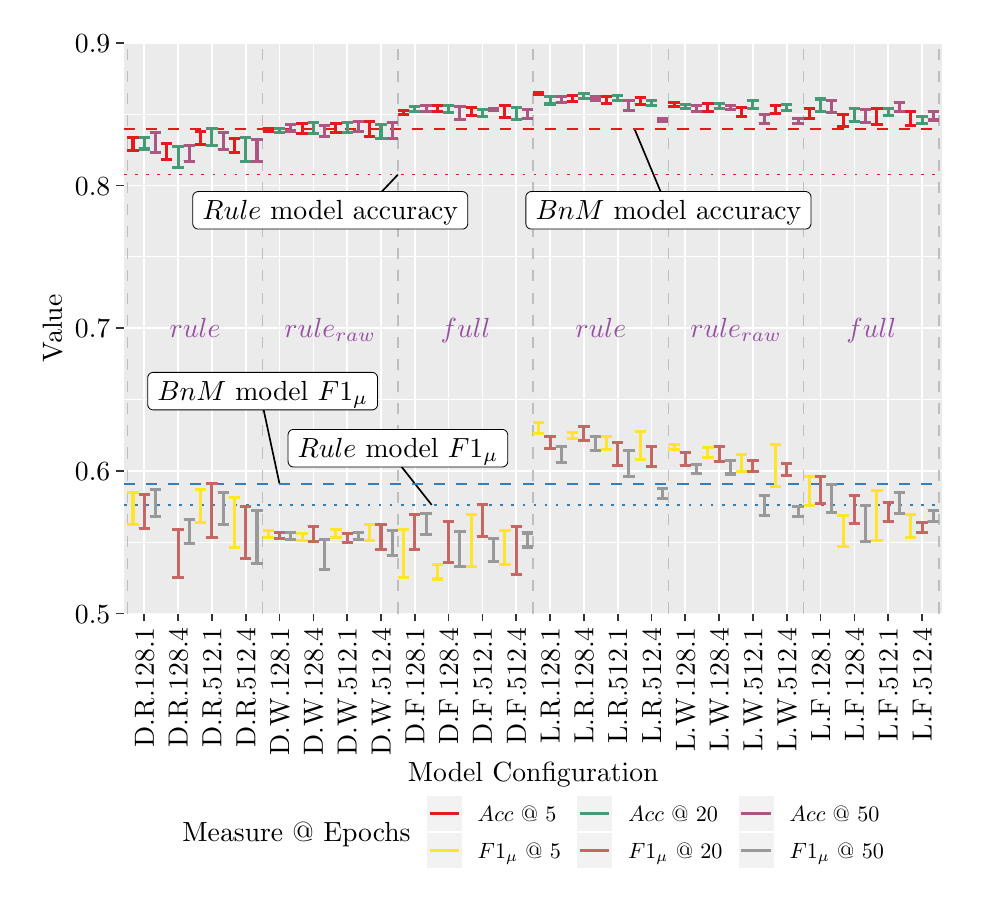
\begin{tikzpicture}[x=1pt,y=1pt]
\definecolor{fillColor}{RGB}{255,255,255}
\path[use as bounding box,fill=fillColor,fill opacity=0.00] (0,0) rectangle (336.00,311.47);
\begin{scope}
\path[clip] (  0.00,  0.00) rectangle (336.00,311.47);
\definecolor{drawColor}{RGB}{255,255,255}
\definecolor{fillColor}{RGB}{255,255,255}

\path[draw=drawColor,line width= 0.6pt,line join=round,line cap=round,fill=fillColor] (  0.00,  0.00) rectangle (336.00,311.47);
\end{scope}
\begin{scope}
\path[clip] ( 34.81, 99.77) rectangle (330.50,305.97);
\definecolor{fillColor}{gray}{0.92}

\path[fill=fillColor] ( 34.81, 99.77) rectangle (330.50,305.97);
\definecolor{drawColor}{RGB}{255,255,255}

\path[draw=drawColor,line width= 0.3pt,line join=round] ( 34.81,125.54) --
	(330.50,125.54);

\path[draw=drawColor,line width= 0.3pt,line join=round] ( 34.81,177.10) --
	(330.50,177.10);

\path[draw=drawColor,line width= 0.3pt,line join=round] ( 34.81,228.65) --
	(330.50,228.65);

\path[draw=drawColor,line width= 0.3pt,line join=round] ( 34.81,280.20) --
	(330.50,280.20);

\path[draw=drawColor,line width= 0.6pt,line join=round] ( 34.81, 99.77) --
	(330.50, 99.77);

\path[draw=drawColor,line width= 0.6pt,line join=round] ( 34.81,151.32) --
	(330.50,151.32);

\path[draw=drawColor,line width= 0.6pt,line join=round] ( 34.81,202.87) --
	(330.50,202.87);

\path[draw=drawColor,line width= 0.6pt,line join=round] ( 34.81,254.42) --
	(330.50,254.42);

\path[draw=drawColor,line width= 0.6pt,line join=round] ( 34.81,305.97) --
	(330.50,305.97);

\path[draw=drawColor,line width= 0.6pt,line join=round] ( 42.14, 99.77) --
	( 42.14,305.97);

\path[draw=drawColor,line width= 0.6pt,line join=round] ( 54.36, 99.77) --
	( 54.36,305.97);

\path[draw=drawColor,line width= 0.6pt,line join=round] ( 66.57, 99.77) --
	( 66.57,305.97);

\path[draw=drawColor,line width= 0.6pt,line join=round] ( 78.79, 99.77) --
	( 78.79,305.97);

\path[draw=drawColor,line width= 0.6pt,line join=round] ( 91.01, 99.77) --
	( 91.01,305.97);

\path[draw=drawColor,line width= 0.6pt,line join=round] (103.23, 99.77) --
	(103.23,305.97);

\path[draw=drawColor,line width= 0.6pt,line join=round] (115.45, 99.77) --
	(115.45,305.97);

\path[draw=drawColor,line width= 0.6pt,line join=round] (127.67, 99.77) --
	(127.67,305.97);

\path[draw=drawColor,line width= 0.6pt,line join=round] (139.89, 99.77) --
	(139.89,305.97);

\path[draw=drawColor,line width= 0.6pt,line join=round] (152.11, 99.77) --
	(152.11,305.97);

\path[draw=drawColor,line width= 0.6pt,line join=round] (164.32, 99.77) --
	(164.32,305.97);

\path[draw=drawColor,line width= 0.6pt,line join=round] (176.54, 99.77) --
	(176.54,305.97);

\path[draw=drawColor,line width= 0.6pt,line join=round] (188.76, 99.77) --
	(188.76,305.97);

\path[draw=drawColor,line width= 0.6pt,line join=round] (200.98, 99.77) --
	(200.98,305.97);

\path[draw=drawColor,line width= 0.6pt,line join=round] (213.20, 99.77) --
	(213.20,305.97);

\path[draw=drawColor,line width= 0.6pt,line join=round] (225.42, 99.77) --
	(225.42,305.97);

\path[draw=drawColor,line width= 0.6pt,line join=round] (237.64, 99.77) --
	(237.64,305.97);

\path[draw=drawColor,line width= 0.6pt,line join=round] (249.86, 99.77) --
	(249.86,305.97);

\path[draw=drawColor,line width= 0.6pt,line join=round] (262.07, 99.77) --
	(262.07,305.97);

\path[draw=drawColor,line width= 0.6pt,line join=round] (274.29, 99.77) --
	(274.29,305.97);

\path[draw=drawColor,line width= 0.6pt,line join=round] (286.51, 99.77) --
	(286.51,305.97);

\path[draw=drawColor,line width= 0.6pt,line join=round] (298.73, 99.77) --
	(298.73,305.97);

\path[draw=drawColor,line width= 0.6pt,line join=round] (310.95, 99.77) --
	(310.95,305.97);

\path[draw=drawColor,line width= 0.6pt,line join=round] (323.17, 99.77) --
	(323.17,305.97);
\definecolor{drawColor}{RGB}{190,190,190}

\path[draw=drawColor,line width= 0.6pt,dash pattern=on 4pt off 4pt ,line join=round] ( 36.03, 99.77) -- ( 36.03,305.97);

\path[draw=drawColor,line width= 0.6pt,dash pattern=on 4pt off 4pt ,line join=round] ( 84.90, 99.77) -- ( 84.90,305.97);

\path[draw=drawColor,line width= 0.6pt,dash pattern=on 4pt off 4pt ,line join=round] (133.78, 99.77) -- (133.78,305.97);

\path[draw=drawColor,line width= 0.6pt,dash pattern=on 4pt off 4pt ,line join=round] (182.65, 99.77) -- (182.65,305.97);

\path[draw=drawColor,line width= 0.6pt,dash pattern=on 4pt off 4pt ,line join=round] (231.53, 99.77) -- (231.53,305.97);

\path[draw=drawColor,line width= 0.6pt,dash pattern=on 4pt off 4pt ,line join=round] (280.40, 99.77) -- (280.40,305.97);

\path[draw=drawColor,line width= 0.6pt,dash pattern=on 4pt off 4pt ,line join=round] (329.28, 99.77) -- (329.28,305.97);
\definecolor{drawColor}{RGB}{152,78,163}

\node[text=drawColor,anchor=base,inner sep=0pt, outer sep=0pt, scale=  1.00] at ( 60.47,199.41) {\(rule\)};

\node[text=drawColor,anchor=base,inner sep=0pt, outer sep=0pt, scale=  1.00] at (109.34,199.41) {\(rule_{raw}\)};

\node[text=drawColor,anchor=base,inner sep=0pt, outer sep=0pt, scale=  1.00] at (158.22,199.41) {\(full\)};

\node[text=drawColor,anchor=base,inner sep=0pt, outer sep=0pt, scale=  1.00] at (207.09,199.41) {\(rule\)};

\node[text=drawColor,anchor=base,inner sep=0pt, outer sep=0pt, scale=  1.00] at (255.97,199.41) {\(rule_{raw}\)};

\node[text=drawColor,anchor=base,inner sep=0pt, outer sep=0pt, scale=  1.00] at (304.84,199.41) {\(full\)};
\definecolor{drawColor}{RGB}{0,0,0}

\path[draw=drawColor,line width= 0.6pt,line join=round] (121.56,245.47) --
	(133.78,258.36);

\path[draw=drawColor,line width= 0.6pt,line join=round] (219.31,274.78) --
	(231.53,245.47);

\path[draw=drawColor,line width= 0.6pt,line join=round] (133.78,154.47) --
	(146.00,139.01);

\path[draw=drawColor,line width= 0.6pt,line join=round] ( 84.90,175.09) --
	( 91.01,146.62);
\definecolor{fillColor}{RGB}{255,255,255}

\path[draw=drawColor,line width= 0.3pt,line join=round,line cap=round,fill=fillColor] ( 45.37,173.36) --
	(124.43,173.36) --
	(124.35,173.36) --
	(124.67,173.37) --
	(124.99,173.44) --
	(125.29,173.55) --
	(125.56,173.71) --
	(125.81,173.91) --
	(126.02,174.15) --
	(126.19,174.42) --
	(126.32,174.72) --
	(126.40,175.03) --
	(126.42,175.35) --
	(126.42,175.35) --
	(126.42,184.91) --
	(126.42,184.91) --
	(126.40,185.23) --
	(126.32,185.54) --
	(126.19,185.83) --
	(126.02,186.10) --
	(125.81,186.34) --
	(125.56,186.55) --
	(125.29,186.71) --
	(124.99,186.82) --
	(124.67,186.88) --
	(124.43,186.90) --
	( 45.37,186.90) --
	( 45.61,186.88) --
	( 45.29,186.90) --
	( 44.97,186.86) --
	( 44.67,186.77) --
	( 44.38,186.63) --
	( 44.11,186.45) --
	( 43.88,186.23) --
	( 43.69,185.97) --
	( 43.54,185.69) --
	( 43.44,185.39) --
	( 43.39,185.07) --
	( 43.38,184.91) --
	( 43.38,175.35) --
	( 43.39,175.51) --
	( 43.39,175.19) --
	( 43.44,174.87) --
	( 43.54,174.57) --
	( 43.69,174.28) --
	( 43.88,174.03) --
	( 44.11,173.81) --
	( 44.38,173.62) --
	( 44.67,173.49) --
	( 44.97,173.40) --
	( 45.29,173.36) --
	cycle;
\end{scope}
\begin{scope}
\path[clip] ( 34.81, 99.77) rectangle (330.50,305.97);
\definecolor{drawColor}{RGB}{0,0,0}

\node[text=drawColor,anchor=base,inner sep=0pt, outer sep=0pt, scale=  1.00] at ( 84.90,176.67) {\(BnM\) model \(F1_\mu\)};
\definecolor{fillColor}{RGB}{255,255,255}

\path[draw=drawColor,line width= 0.3pt,line join=round,line cap=round,fill=fillColor] ( 96.08,152.74) --
	(171.48,152.74) --
	(171.40,152.74) --
	(171.72,152.75) --
	(172.03,152.82) --
	(172.33,152.93) --
	(172.61,153.09) --
	(172.85,153.29) --
	(173.07,153.53) --
	(173.24,153.80) --
	(173.36,154.10) --
	(173.44,154.41) --
	(173.47,154.73) --
	(173.47,154.73) --
	(173.47,164.29) --
	(173.47,164.29) --
	(173.44,164.61) --
	(173.36,164.92) --
	(173.24,165.21) --
	(173.07,165.48) --
	(172.85,165.72) --
	(172.61,165.93) --
	(172.33,166.09) --
	(172.03,166.20) --
	(171.72,166.26) --
	(171.48,166.28) --
	( 96.08,166.28) --
	( 96.32,166.26) --
	( 96.00,166.28) --
	( 95.68,166.24) --
	( 95.37,166.15) --
	( 95.08,166.01) --
	( 94.82,165.83) --
	( 94.59,165.61) --
	( 94.40,165.35) --
	( 94.25,165.07) --
	( 94.15,164.77) --
	( 94.10,164.45) --
	( 94.09,164.29) --
	( 94.09,154.73) --
	( 94.10,154.89) --
	( 94.10,154.57) --
	( 94.15,154.25) --
	( 94.25,153.95) --
	( 94.40,153.66) --
	( 94.59,153.41) --
	( 94.82,153.19) --
	( 95.08,153.00) --
	( 95.37,152.87) --
	( 95.68,152.78) --
	( 96.00,152.74) --
	cycle;
\end{scope}
\begin{scope}
\path[clip] ( 34.81, 99.77) rectangle (330.50,305.97);
\definecolor{drawColor}{RGB}{0,0,0}

\node[text=drawColor,anchor=base,inner sep=0pt, outer sep=0pt, scale=  1.00] at (133.78,156.05) {\(Rule\) model \(F1_\mu\)};
\definecolor{fillColor}{RGB}{255,255,255}

\path[draw=drawColor,line width= 0.3pt,line join=round,line cap=round,fill=fillColor] ( 61.65,238.70) --
	(157.03,238.70) --
	(156.95,238.70) --
	(157.27,238.72) --
	(157.58,238.78) --
	(157.88,238.89) --
	(158.16,239.05) --
	(158.40,239.26) --
	(158.62,239.50) --
	(158.79,239.77) --
	(158.91,240.06) --
	(158.99,240.37) --
	(159.01,240.69) --
	(159.01,240.69) --
	(159.01,250.25) --
	(159.01,250.25) --
	(158.99,250.57) --
	(158.91,250.88) --
	(158.79,251.18) --
	(158.62,251.45) --
	(158.40,251.69) --
	(158.16,251.89) --
	(157.88,252.05) --
	(157.58,252.16) --
	(157.27,252.23) --
	(157.03,252.24) --
	( 61.65,252.24) --
	( 61.89,252.23) --
	( 61.57,252.24) --
	( 61.26,252.20) --
	( 60.95,252.11) --
	( 60.66,251.97) --
	( 60.40,251.79) --
	( 60.17,251.57) --
	( 59.97,251.32) --
	( 59.83,251.03) --
	( 59.72,250.73) --
	( 59.67,250.41) --
	( 59.67,250.25) --
	( 59.67,240.69) --
	( 59.67,240.85) --
	( 59.67,240.53) --
	( 59.72,240.21) --
	( 59.83,239.91) --
	( 59.97,239.63) --
	( 60.17,239.37) --
	( 60.40,239.15) --
	( 60.66,238.97) --
	( 60.95,238.83) --
	( 61.26,238.74) --
	( 61.57,238.70) --
	cycle;
\end{scope}
\begin{scope}
\path[clip] ( 34.81, 99.77) rectangle (330.50,305.97);
\definecolor{drawColor}{RGB}{0,0,0}

\node[text=drawColor,anchor=base,inner sep=0pt, outer sep=0pt, scale=  1.00] at (109.34,242.01) {\(Rule\) model accuracy};
\definecolor{fillColor}{RGB}{255,255,255}

\path[draw=drawColor,line width= 0.3pt,line join=round,line cap=round,fill=fillColor] (182.01,238.70) --
	(281.05,238.70) --
	(280.97,238.70) --
	(281.29,238.72) --
	(281.60,238.78) --
	(281.90,238.89) --
	(282.17,239.05) --
	(282.42,239.26) --
	(282.63,239.50) --
	(282.81,239.77) --
	(282.93,240.06) --
	(283.01,240.37) --
	(283.03,240.69) --
	(283.03,240.69) --
	(283.03,250.25) --
	(283.03,250.25) --
	(283.01,250.57) --
	(282.93,250.88) --
	(282.81,251.18) --
	(282.63,251.45) --
	(282.42,251.69) --
	(282.17,251.89) --
	(281.90,252.05) --
	(281.60,252.16) --
	(281.29,252.23) --
	(281.05,252.24) --
	(182.01,252.24) --
	(182.25,252.23) --
	(181.93,252.24) --
	(181.61,252.20) --
	(181.31,252.11) --
	(181.02,251.97) --
	(180.75,251.79) --
	(180.52,251.57) --
	(180.33,251.32) --
	(180.18,251.03) --
	(180.08,250.73) --
	(180.03,250.41) --
	(180.02,250.25) --
	(180.02,240.69) --
	(180.03,240.85) --
	(180.03,240.53) --
	(180.08,240.21) --
	(180.18,239.91) --
	(180.33,239.63) --
	(180.52,239.37) --
	(180.75,239.15) --
	(181.02,238.97) --
	(181.31,238.83) --
	(181.61,238.74) --
	(181.93,238.70) --
	cycle;
\end{scope}
\begin{scope}
\path[clip] ( 34.81, 99.77) rectangle (330.50,305.97);
\definecolor{drawColor}{RGB}{0,0,0}

\node[text=drawColor,anchor=base,inner sep=0pt, outer sep=0pt, scale=  1.00] at (231.53,242.01) {\(BnM\) model accuracy};
\definecolor{drawColor}{RGB}{228,26,28}

\path[draw=drawColor,line width= 0.6pt,dash pattern=on 4pt off 4pt ,line join=round] ( 34.81,274.78) -- (330.50,274.78);

\path[draw=drawColor,line width= 0.6pt,dash pattern=on 1pt off 3pt ,line join=round] ( 34.81,258.36) -- (330.50,258.36);
\definecolor{drawColor}{RGB}{55,126,184}

\path[draw=drawColor,line width= 0.6pt,dash pattern=on 4pt off 4pt ,line join=round] ( 34.81,146.62) -- (330.50,146.62);

\path[draw=drawColor,line width= 0.6pt,dash pattern=on 1pt off 3pt ,line join=round] ( 34.81,139.01) -- (330.50,139.01);
\definecolor{drawColor}{RGB}{172,87,130}

\path[draw=drawColor,line width= 1.1pt,line join=round] ( 44.17,273.65) --
	( 48.25,273.65);

\path[draw=drawColor,line width= 1.1pt,line join=round] ( 46.21,273.65) --
	( 46.21,266.20);

\path[draw=drawColor,line width= 1.1pt,line join=round] ( 44.17,266.20) --
	( 48.25,266.20);

\path[draw=drawColor,line width= 1.1pt,line join=round] ( 44.17,273.65) --
	( 48.25,273.65);

\path[draw=drawColor,line width= 1.1pt,line join=round] ( 46.21,273.65) --
	( 46.21,266.20);

\path[draw=drawColor,line width= 1.1pt,line join=round] ( 44.17,266.20) --
	( 48.25,266.20);

\path[draw=drawColor,line width= 1.1pt,line join=round] ( 44.17,273.65) --
	( 48.25,273.65);

\path[draw=drawColor,line width= 1.1pt,line join=round] ( 46.21,273.65) --
	( 46.21,266.20);

\path[draw=drawColor,line width= 1.1pt,line join=round] ( 44.17,266.20) --
	( 48.25,266.20);

\path[draw=drawColor,line width= 1.1pt,line join=round] ( 44.17,273.65) --
	( 48.25,273.65);

\path[draw=drawColor,line width= 1.1pt,line join=round] ( 46.21,273.65) --
	( 46.21,266.20);

\path[draw=drawColor,line width= 1.1pt,line join=round] ( 44.17,266.20) --
	( 48.25,266.20);

\path[draw=drawColor,line width= 1.1pt,line join=round] ( 44.17,273.65) --
	( 48.25,273.65);

\path[draw=drawColor,line width= 1.1pt,line join=round] ( 46.21,273.65) --
	( 46.21,266.20);

\path[draw=drawColor,line width= 1.1pt,line join=round] ( 44.17,266.20) --
	( 48.25,266.20);

\path[draw=drawColor,line width= 1.1pt,line join=round] ( 44.17,273.65) --
	( 48.25,273.65);

\path[draw=drawColor,line width= 1.1pt,line join=round] ( 46.21,273.65) --
	( 46.21,266.20);

\path[draw=drawColor,line width= 1.1pt,line join=round] ( 44.17,266.20) --
	( 48.25,266.20);

\path[draw=drawColor,line width= 1.1pt,line join=round] ( 44.17,273.65) --
	( 48.25,273.65);

\path[draw=drawColor,line width= 1.1pt,line join=round] ( 46.21,273.65) --
	( 46.21,266.20);

\path[draw=drawColor,line width= 1.1pt,line join=round] ( 44.17,266.20) --
	( 48.25,266.20);

\path[draw=drawColor,line width= 1.1pt,line join=round] ( 44.17,273.65) --
	( 48.25,273.65);

\path[draw=drawColor,line width= 1.1pt,line join=round] ( 46.21,273.65) --
	( 46.21,266.20);

\path[draw=drawColor,line width= 1.1pt,line join=round] ( 44.17,266.20) --
	( 48.25,266.20);
\definecolor{drawColor}{RGB}{68,155,117}

\path[draw=drawColor,line width= 1.1pt,line join=round] ( 40.10,271.74) --
	( 44.17,271.74);

\path[draw=drawColor,line width= 1.1pt,line join=round] ( 42.14,271.74) --
	( 42.14,267.63);

\path[draw=drawColor,line width= 1.1pt,line join=round] ( 40.10,267.63) --
	( 44.17,267.63);

\path[draw=drawColor,line width= 1.1pt,line join=round] ( 40.10,271.74) --
	( 44.17,271.74);

\path[draw=drawColor,line width= 1.1pt,line join=round] ( 42.14,271.74) --
	( 42.14,267.63);

\path[draw=drawColor,line width= 1.1pt,line join=round] ( 40.10,267.63) --
	( 44.17,267.63);

\path[draw=drawColor,line width= 1.1pt,line join=round] ( 40.10,271.74) --
	( 44.17,271.74);

\path[draw=drawColor,line width= 1.1pt,line join=round] ( 42.14,271.74) --
	( 42.14,267.63);

\path[draw=drawColor,line width= 1.1pt,line join=round] ( 40.10,267.63) --
	( 44.17,267.63);

\path[draw=drawColor,line width= 1.1pt,line join=round] ( 40.10,271.74) --
	( 44.17,271.74);

\path[draw=drawColor,line width= 1.1pt,line join=round] ( 42.14,271.74) --
	( 42.14,267.63);

\path[draw=drawColor,line width= 1.1pt,line join=round] ( 40.10,267.63) --
	( 44.17,267.63);

\path[draw=drawColor,line width= 1.1pt,line join=round] ( 40.10,271.74) --
	( 44.17,271.74);

\path[draw=drawColor,line width= 1.1pt,line join=round] ( 42.14,271.74) --
	( 42.14,267.63);

\path[draw=drawColor,line width= 1.1pt,line join=round] ( 40.10,267.63) --
	( 44.17,267.63);

\path[draw=drawColor,line width= 1.1pt,line join=round] ( 40.10,271.74) --
	( 44.17,271.74);

\path[draw=drawColor,line width= 1.1pt,line join=round] ( 42.14,271.74) --
	( 42.14,267.63);

\path[draw=drawColor,line width= 1.1pt,line join=round] ( 40.10,267.63) --
	( 44.17,267.63);

\path[draw=drawColor,line width= 1.1pt,line join=round] ( 40.10,271.74) --
	( 44.17,271.74);

\path[draw=drawColor,line width= 1.1pt,line join=round] ( 42.14,271.74) --
	( 42.14,267.63);

\path[draw=drawColor,line width= 1.1pt,line join=round] ( 40.10,267.63) --
	( 44.17,267.63);

\path[draw=drawColor,line width= 1.1pt,line join=round] ( 40.10,271.74) --
	( 44.17,271.74);

\path[draw=drawColor,line width= 1.1pt,line join=round] ( 42.14,271.74) --
	( 42.14,267.63);

\path[draw=drawColor,line width= 1.1pt,line join=round] ( 40.10,267.63) --
	( 44.17,267.63);
\definecolor{drawColor}{RGB}{228,26,28}

\path[draw=drawColor,line width= 1.1pt,line join=round] ( 36.03,271.71) --
	( 40.10,271.71);

\path[draw=drawColor,line width= 1.1pt,line join=round] ( 38.06,271.71) --
	( 38.06,267.11);

\path[draw=drawColor,line width= 1.1pt,line join=round] ( 36.03,267.11) --
	( 40.10,267.11);

\path[draw=drawColor,line width= 1.1pt,line join=round] ( 36.03,271.71) --
	( 40.10,271.71);

\path[draw=drawColor,line width= 1.1pt,line join=round] ( 38.06,271.71) --
	( 38.06,267.11);

\path[draw=drawColor,line width= 1.1pt,line join=round] ( 36.03,267.11) --
	( 40.10,267.11);

\path[draw=drawColor,line width= 1.1pt,line join=round] ( 36.03,271.71) --
	( 40.10,271.71);

\path[draw=drawColor,line width= 1.1pt,line join=round] ( 38.06,271.71) --
	( 38.06,267.11);

\path[draw=drawColor,line width= 1.1pt,line join=round] ( 36.03,267.11) --
	( 40.10,267.11);

\path[draw=drawColor,line width= 1.1pt,line join=round] ( 36.03,271.71) --
	( 40.10,271.71);

\path[draw=drawColor,line width= 1.1pt,line join=round] ( 38.06,271.71) --
	( 38.06,267.11);

\path[draw=drawColor,line width= 1.1pt,line join=round] ( 36.03,267.11) --
	( 40.10,267.11);

\path[draw=drawColor,line width= 1.1pt,line join=round] ( 36.03,271.71) --
	( 40.10,271.71);

\path[draw=drawColor,line width= 1.1pt,line join=round] ( 38.06,271.71) --
	( 38.06,267.11);

\path[draw=drawColor,line width= 1.1pt,line join=round] ( 36.03,267.11) --
	( 40.10,267.11);

\path[draw=drawColor,line width= 1.1pt,line join=round] ( 36.03,271.71) --
	( 40.10,271.71);

\path[draw=drawColor,line width= 1.1pt,line join=round] ( 38.06,271.71) --
	( 38.06,267.11);

\path[draw=drawColor,line width= 1.1pt,line join=round] ( 36.03,267.11) --
	( 40.10,267.11);

\path[draw=drawColor,line width= 1.1pt,line join=round] ( 36.03,271.71) --
	( 40.10,271.71);

\path[draw=drawColor,line width= 1.1pt,line join=round] ( 38.06,271.71) --
	( 38.06,267.11);

\path[draw=drawColor,line width= 1.1pt,line join=round] ( 36.03,267.11) --
	( 40.10,267.11);

\path[draw=drawColor,line width= 1.1pt,line join=round] ( 36.03,271.71) --
	( 40.10,271.71);

\path[draw=drawColor,line width= 1.1pt,line join=round] ( 38.06,271.71) --
	( 38.06,267.11);

\path[draw=drawColor,line width= 1.1pt,line join=round] ( 36.03,267.11) --
	( 40.10,267.11);
\definecolor{drawColor}{RGB}{172,87,130}

\path[draw=drawColor,line width= 1.1pt,line join=round] ( 56.39,269.00) --
	( 60.47,269.00);

\path[draw=drawColor,line width= 1.1pt,line join=round] ( 58.43,269.00) --
	( 58.43,263.17);

\path[draw=drawColor,line width= 1.1pt,line join=round] ( 56.39,263.17) --
	( 60.47,263.17);

\path[draw=drawColor,line width= 1.1pt,line join=round] ( 56.39,269.00) --
	( 60.47,269.00);

\path[draw=drawColor,line width= 1.1pt,line join=round] ( 58.43,269.00) --
	( 58.43,263.17);

\path[draw=drawColor,line width= 1.1pt,line join=round] ( 56.39,263.17) --
	( 60.47,263.17);

\path[draw=drawColor,line width= 1.1pt,line join=round] ( 56.39,269.00) --
	( 60.47,269.00);

\path[draw=drawColor,line width= 1.1pt,line join=round] ( 58.43,269.00) --
	( 58.43,263.17);

\path[draw=drawColor,line width= 1.1pt,line join=round] ( 56.39,263.17) --
	( 60.47,263.17);

\path[draw=drawColor,line width= 1.1pt,line join=round] ( 56.39,269.00) --
	( 60.47,269.00);

\path[draw=drawColor,line width= 1.1pt,line join=round] ( 58.43,269.00) --
	( 58.43,263.17);

\path[draw=drawColor,line width= 1.1pt,line join=round] ( 56.39,263.17) --
	( 60.47,263.17);

\path[draw=drawColor,line width= 1.1pt,line join=round] ( 56.39,269.00) --
	( 60.47,269.00);

\path[draw=drawColor,line width= 1.1pt,line join=round] ( 58.43,269.00) --
	( 58.43,263.17);

\path[draw=drawColor,line width= 1.1pt,line join=round] ( 56.39,263.17) --
	( 60.47,263.17);

\path[draw=drawColor,line width= 1.1pt,line join=round] ( 56.39,269.00) --
	( 60.47,269.00);

\path[draw=drawColor,line width= 1.1pt,line join=round] ( 58.43,269.00) --
	( 58.43,263.17);

\path[draw=drawColor,line width= 1.1pt,line join=round] ( 56.39,263.17) --
	( 60.47,263.17);

\path[draw=drawColor,line width= 1.1pt,line join=round] ( 56.39,269.00) --
	( 60.47,269.00);

\path[draw=drawColor,line width= 1.1pt,line join=round] ( 58.43,269.00) --
	( 58.43,263.17);

\path[draw=drawColor,line width= 1.1pt,line join=round] ( 56.39,263.17) --
	( 60.47,263.17);

\path[draw=drawColor,line width= 1.1pt,line join=round] ( 56.39,269.00) --
	( 60.47,269.00);

\path[draw=drawColor,line width= 1.1pt,line join=round] ( 58.43,269.00) --
	( 58.43,263.17);

\path[draw=drawColor,line width= 1.1pt,line join=round] ( 56.39,263.17) --
	( 60.47,263.17);
\definecolor{drawColor}{RGB}{68,155,117}

\path[draw=drawColor,line width= 1.1pt,line join=round] ( 52.32,268.59) --
	( 56.39,268.59);

\path[draw=drawColor,line width= 1.1pt,line join=round] ( 54.36,268.59) --
	( 54.36,261.01);

\path[draw=drawColor,line width= 1.1pt,line join=round] ( 52.32,261.01) --
	( 56.39,261.01);

\path[draw=drawColor,line width= 1.1pt,line join=round] ( 52.32,268.59) --
	( 56.39,268.59);

\path[draw=drawColor,line width= 1.1pt,line join=round] ( 54.36,268.59) --
	( 54.36,261.01);

\path[draw=drawColor,line width= 1.1pt,line join=round] ( 52.32,261.01) --
	( 56.39,261.01);

\path[draw=drawColor,line width= 1.1pt,line join=round] ( 52.32,268.59) --
	( 56.39,268.59);

\path[draw=drawColor,line width= 1.1pt,line join=round] ( 54.36,268.59) --
	( 54.36,261.01);

\path[draw=drawColor,line width= 1.1pt,line join=round] ( 52.32,261.01) --
	( 56.39,261.01);

\path[draw=drawColor,line width= 1.1pt,line join=round] ( 52.32,268.59) --
	( 56.39,268.59);

\path[draw=drawColor,line width= 1.1pt,line join=round] ( 54.36,268.59) --
	( 54.36,261.01);

\path[draw=drawColor,line width= 1.1pt,line join=round] ( 52.32,261.01) --
	( 56.39,261.01);

\path[draw=drawColor,line width= 1.1pt,line join=round] ( 52.32,268.59) --
	( 56.39,268.59);

\path[draw=drawColor,line width= 1.1pt,line join=round] ( 54.36,268.59) --
	( 54.36,261.01);

\path[draw=drawColor,line width= 1.1pt,line join=round] ( 52.32,261.01) --
	( 56.39,261.01);

\path[draw=drawColor,line width= 1.1pt,line join=round] ( 52.32,268.59) --
	( 56.39,268.59);

\path[draw=drawColor,line width= 1.1pt,line join=round] ( 54.36,268.59) --
	( 54.36,261.01);

\path[draw=drawColor,line width= 1.1pt,line join=round] ( 52.32,261.01) --
	( 56.39,261.01);

\path[draw=drawColor,line width= 1.1pt,line join=round] ( 52.32,268.59) --
	( 56.39,268.59);

\path[draw=drawColor,line width= 1.1pt,line join=round] ( 54.36,268.59) --
	( 54.36,261.01);

\path[draw=drawColor,line width= 1.1pt,line join=round] ( 52.32,261.01) --
	( 56.39,261.01);

\path[draw=drawColor,line width= 1.1pt,line join=round] ( 52.32,268.59) --
	( 56.39,268.59);

\path[draw=drawColor,line width= 1.1pt,line join=round] ( 54.36,268.59) --
	( 54.36,261.01);

\path[draw=drawColor,line width= 1.1pt,line join=round] ( 52.32,261.01) --
	( 56.39,261.01);
\definecolor{drawColor}{RGB}{228,26,28}

\path[draw=drawColor,line width= 1.1pt,line join=round] ( 48.25,269.65) --
	( 52.32,269.65);

\path[draw=drawColor,line width= 1.1pt,line join=round] ( 50.28,269.65) --
	( 50.28,263.71);

\path[draw=drawColor,line width= 1.1pt,line join=round] ( 48.25,263.71) --
	( 52.32,263.71);

\path[draw=drawColor,line width= 1.1pt,line join=round] ( 48.25,269.65) --
	( 52.32,269.65);

\path[draw=drawColor,line width= 1.1pt,line join=round] ( 50.28,269.65) --
	( 50.28,263.71);

\path[draw=drawColor,line width= 1.1pt,line join=round] ( 48.25,263.71) --
	( 52.32,263.71);

\path[draw=drawColor,line width= 1.1pt,line join=round] ( 48.25,269.65) --
	( 52.32,269.65);

\path[draw=drawColor,line width= 1.1pt,line join=round] ( 50.28,269.65) --
	( 50.28,263.71);

\path[draw=drawColor,line width= 1.1pt,line join=round] ( 48.25,263.71) --
	( 52.32,263.71);

\path[draw=drawColor,line width= 1.1pt,line join=round] ( 48.25,269.65) --
	( 52.32,269.65);

\path[draw=drawColor,line width= 1.1pt,line join=round] ( 50.28,269.65) --
	( 50.28,263.71);

\path[draw=drawColor,line width= 1.1pt,line join=round] ( 48.25,263.71) --
	( 52.32,263.71);

\path[draw=drawColor,line width= 1.1pt,line join=round] ( 48.25,269.65) --
	( 52.32,269.65);

\path[draw=drawColor,line width= 1.1pt,line join=round] ( 50.28,269.65) --
	( 50.28,263.71);

\path[draw=drawColor,line width= 1.1pt,line join=round] ( 48.25,263.71) --
	( 52.32,263.71);

\path[draw=drawColor,line width= 1.1pt,line join=round] ( 48.25,269.65) --
	( 52.32,269.65);

\path[draw=drawColor,line width= 1.1pt,line join=round] ( 50.28,269.65) --
	( 50.28,263.71);

\path[draw=drawColor,line width= 1.1pt,line join=round] ( 48.25,263.71) --
	( 52.32,263.71);

\path[draw=drawColor,line width= 1.1pt,line join=round] ( 48.25,269.65) --
	( 52.32,269.65);

\path[draw=drawColor,line width= 1.1pt,line join=round] ( 50.28,269.65) --
	( 50.28,263.71);

\path[draw=drawColor,line width= 1.1pt,line join=round] ( 48.25,263.71) --
	( 52.32,263.71);

\path[draw=drawColor,line width= 1.1pt,line join=round] ( 48.25,269.65) --
	( 52.32,269.65);

\path[draw=drawColor,line width= 1.1pt,line join=round] ( 50.28,269.65) --
	( 50.28,263.71);

\path[draw=drawColor,line width= 1.1pt,line join=round] ( 48.25,263.71) --
	( 52.32,263.71);
\definecolor{drawColor}{RGB}{172,87,130}

\path[draw=drawColor,line width= 1.1pt,line join=round] ( 68.61,273.53) --
	( 72.68,273.53);

\path[draw=drawColor,line width= 1.1pt,line join=round] ( 70.65,273.53) --
	( 70.65,267.33);

\path[draw=drawColor,line width= 1.1pt,line join=round] ( 68.61,267.33) --
	( 72.68,267.33);

\path[draw=drawColor,line width= 1.1pt,line join=round] ( 68.61,273.53) --
	( 72.68,273.53);

\path[draw=drawColor,line width= 1.1pt,line join=round] ( 70.65,273.53) --
	( 70.65,267.33);

\path[draw=drawColor,line width= 1.1pt,line join=round] ( 68.61,267.33) --
	( 72.68,267.33);

\path[draw=drawColor,line width= 1.1pt,line join=round] ( 68.61,273.53) --
	( 72.68,273.53);

\path[draw=drawColor,line width= 1.1pt,line join=round] ( 70.65,273.53) --
	( 70.65,267.33);

\path[draw=drawColor,line width= 1.1pt,line join=round] ( 68.61,267.33) --
	( 72.68,267.33);

\path[draw=drawColor,line width= 1.1pt,line join=round] ( 68.61,273.53) --
	( 72.68,273.53);

\path[draw=drawColor,line width= 1.1pt,line join=round] ( 70.65,273.53) --
	( 70.65,267.33);

\path[draw=drawColor,line width= 1.1pt,line join=round] ( 68.61,267.33) --
	( 72.68,267.33);

\path[draw=drawColor,line width= 1.1pt,line join=round] ( 68.61,273.53) --
	( 72.68,273.53);

\path[draw=drawColor,line width= 1.1pt,line join=round] ( 70.65,273.53) --
	( 70.65,267.33);

\path[draw=drawColor,line width= 1.1pt,line join=round] ( 68.61,267.33) --
	( 72.68,267.33);

\path[draw=drawColor,line width= 1.1pt,line join=round] ( 68.61,273.53) --
	( 72.68,273.53);

\path[draw=drawColor,line width= 1.1pt,line join=round] ( 70.65,273.53) --
	( 70.65,267.33);

\path[draw=drawColor,line width= 1.1pt,line join=round] ( 68.61,267.33) --
	( 72.68,267.33);

\path[draw=drawColor,line width= 1.1pt,line join=round] ( 68.61,273.53) --
	( 72.68,273.53);

\path[draw=drawColor,line width= 1.1pt,line join=round] ( 70.65,273.53) --
	( 70.65,267.33);

\path[draw=drawColor,line width= 1.1pt,line join=round] ( 68.61,267.33) --
	( 72.68,267.33);

\path[draw=drawColor,line width= 1.1pt,line join=round] ( 68.61,273.53) --
	( 72.68,273.53);

\path[draw=drawColor,line width= 1.1pt,line join=round] ( 70.65,273.53) --
	( 70.65,267.33);

\path[draw=drawColor,line width= 1.1pt,line join=round] ( 68.61,267.33) --
	( 72.68,267.33);
\definecolor{drawColor}{RGB}{68,155,117}

\path[draw=drawColor,line width= 1.1pt,line join=round] ( 64.54,274.95) --
	( 68.61,274.95);

\path[draw=drawColor,line width= 1.1pt,line join=round] ( 66.57,274.95) --
	( 66.57,268.85);

\path[draw=drawColor,line width= 1.1pt,line join=round] ( 64.54,268.85) --
	( 68.61,268.85);

\path[draw=drawColor,line width= 1.1pt,line join=round] ( 64.54,274.95) --
	( 68.61,274.95);

\path[draw=drawColor,line width= 1.1pt,line join=round] ( 66.57,274.95) --
	( 66.57,268.85);

\path[draw=drawColor,line width= 1.1pt,line join=round] ( 64.54,268.85) --
	( 68.61,268.85);

\path[draw=drawColor,line width= 1.1pt,line join=round] ( 64.54,274.95) --
	( 68.61,274.95);

\path[draw=drawColor,line width= 1.1pt,line join=round] ( 66.57,274.95) --
	( 66.57,268.85);

\path[draw=drawColor,line width= 1.1pt,line join=round] ( 64.54,268.85) --
	( 68.61,268.85);

\path[draw=drawColor,line width= 1.1pt,line join=round] ( 64.54,274.95) --
	( 68.61,274.95);

\path[draw=drawColor,line width= 1.1pt,line join=round] ( 66.57,274.95) --
	( 66.57,268.85);

\path[draw=drawColor,line width= 1.1pt,line join=round] ( 64.54,268.85) --
	( 68.61,268.85);

\path[draw=drawColor,line width= 1.1pt,line join=round] ( 64.54,274.95) --
	( 68.61,274.95);

\path[draw=drawColor,line width= 1.1pt,line join=round] ( 66.57,274.95) --
	( 66.57,268.85);

\path[draw=drawColor,line width= 1.1pt,line join=round] ( 64.54,268.85) --
	( 68.61,268.85);

\path[draw=drawColor,line width= 1.1pt,line join=round] ( 64.54,274.95) --
	( 68.61,274.95);

\path[draw=drawColor,line width= 1.1pt,line join=round] ( 66.57,274.95) --
	( 66.57,268.85);

\path[draw=drawColor,line width= 1.1pt,line join=round] ( 64.54,268.85) --
	( 68.61,268.85);

\path[draw=drawColor,line width= 1.1pt,line join=round] ( 64.54,274.95) --
	( 68.61,274.95);

\path[draw=drawColor,line width= 1.1pt,line join=round] ( 66.57,274.95) --
	( 66.57,268.85);

\path[draw=drawColor,line width= 1.1pt,line join=round] ( 64.54,268.85) --
	( 68.61,268.85);

\path[draw=drawColor,line width= 1.1pt,line join=round] ( 64.54,274.95) --
	( 68.61,274.95);

\path[draw=drawColor,line width= 1.1pt,line join=round] ( 66.57,274.95) --
	( 66.57,268.85);

\path[draw=drawColor,line width= 1.1pt,line join=round] ( 64.54,268.85) --
	( 68.61,268.85);
\definecolor{drawColor}{RGB}{228,26,28}

\path[draw=drawColor,line width= 1.1pt,line join=round] ( 60.47,273.98) --
	( 64.54,273.98);

\path[draw=drawColor,line width= 1.1pt,line join=round] ( 62.50,273.98) --
	( 62.50,269.16);

\path[draw=drawColor,line width= 1.1pt,line join=round] ( 60.47,269.16) --
	( 64.54,269.16);

\path[draw=drawColor,line width= 1.1pt,line join=round] ( 60.47,273.98) --
	( 64.54,273.98);

\path[draw=drawColor,line width= 1.1pt,line join=round] ( 62.50,273.98) --
	( 62.50,269.16);

\path[draw=drawColor,line width= 1.1pt,line join=round] ( 60.47,269.16) --
	( 64.54,269.16);

\path[draw=drawColor,line width= 1.1pt,line join=round] ( 60.47,273.98) --
	( 64.54,273.98);

\path[draw=drawColor,line width= 1.1pt,line join=round] ( 62.50,273.98) --
	( 62.50,269.16);

\path[draw=drawColor,line width= 1.1pt,line join=round] ( 60.47,269.16) --
	( 64.54,269.16);

\path[draw=drawColor,line width= 1.1pt,line join=round] ( 60.47,273.98) --
	( 64.54,273.98);

\path[draw=drawColor,line width= 1.1pt,line join=round] ( 62.50,273.98) --
	( 62.50,269.16);

\path[draw=drawColor,line width= 1.1pt,line join=round] ( 60.47,269.16) --
	( 64.54,269.16);

\path[draw=drawColor,line width= 1.1pt,line join=round] ( 60.47,273.98) --
	( 64.54,273.98);

\path[draw=drawColor,line width= 1.1pt,line join=round] ( 62.50,273.98) --
	( 62.50,269.16);

\path[draw=drawColor,line width= 1.1pt,line join=round] ( 60.47,269.16) --
	( 64.54,269.16);

\path[draw=drawColor,line width= 1.1pt,line join=round] ( 60.47,273.98) --
	( 64.54,273.98);

\path[draw=drawColor,line width= 1.1pt,line join=round] ( 62.50,273.98) --
	( 62.50,269.16);

\path[draw=drawColor,line width= 1.1pt,line join=round] ( 60.47,269.16) --
	( 64.54,269.16);

\path[draw=drawColor,line width= 1.1pt,line join=round] ( 60.47,273.98) --
	( 64.54,273.98);

\path[draw=drawColor,line width= 1.1pt,line join=round] ( 62.50,273.98) --
	( 62.50,269.16);

\path[draw=drawColor,line width= 1.1pt,line join=round] ( 60.47,269.16) --
	( 64.54,269.16);

\path[draw=drawColor,line width= 1.1pt,line join=round] ( 60.47,273.98) --
	( 64.54,273.98);

\path[draw=drawColor,line width= 1.1pt,line join=round] ( 62.50,273.98) --
	( 62.50,269.16);

\path[draw=drawColor,line width= 1.1pt,line join=round] ( 60.47,269.16) --
	( 64.54,269.16);
\definecolor{drawColor}{RGB}{172,87,130}

\path[draw=drawColor,line width= 1.1pt,line join=round] ( 80.83,271.04) --
	( 84.90,271.04);

\path[draw=drawColor,line width= 1.1pt,line join=round] ( 82.87,271.04) --
	( 82.87,263.06);

\path[draw=drawColor,line width= 1.1pt,line join=round] ( 80.83,263.06) --
	( 84.90,263.06);

\path[draw=drawColor,line width= 1.1pt,line join=round] ( 80.83,271.04) --
	( 84.90,271.04);

\path[draw=drawColor,line width= 1.1pt,line join=round] ( 82.87,271.04) --
	( 82.87,263.06);

\path[draw=drawColor,line width= 1.1pt,line join=round] ( 80.83,263.06) --
	( 84.90,263.06);

\path[draw=drawColor,line width= 1.1pt,line join=round] ( 80.83,271.04) --
	( 84.90,271.04);

\path[draw=drawColor,line width= 1.1pt,line join=round] ( 82.87,271.04) --
	( 82.87,263.06);

\path[draw=drawColor,line width= 1.1pt,line join=round] ( 80.83,263.06) --
	( 84.90,263.06);

\path[draw=drawColor,line width= 1.1pt,line join=round] ( 80.83,271.04) --
	( 84.90,271.04);

\path[draw=drawColor,line width= 1.1pt,line join=round] ( 82.87,271.04) --
	( 82.87,263.06);

\path[draw=drawColor,line width= 1.1pt,line join=round] ( 80.83,263.06) --
	( 84.90,263.06);

\path[draw=drawColor,line width= 1.1pt,line join=round] ( 80.83,271.04) --
	( 84.90,271.04);

\path[draw=drawColor,line width= 1.1pt,line join=round] ( 82.87,271.04) --
	( 82.87,263.06);

\path[draw=drawColor,line width= 1.1pt,line join=round] ( 80.83,263.06) --
	( 84.90,263.06);

\path[draw=drawColor,line width= 1.1pt,line join=round] ( 80.83,271.04) --
	( 84.90,271.04);

\path[draw=drawColor,line width= 1.1pt,line join=round] ( 82.87,271.04) --
	( 82.87,263.06);

\path[draw=drawColor,line width= 1.1pt,line join=round] ( 80.83,263.06) --
	( 84.90,263.06);

\path[draw=drawColor,line width= 1.1pt,line join=round] ( 80.83,271.04) --
	( 84.90,271.04);

\path[draw=drawColor,line width= 1.1pt,line join=round] ( 82.87,271.04) --
	( 82.87,263.06);

\path[draw=drawColor,line width= 1.1pt,line join=round] ( 80.83,263.06) --
	( 84.90,263.06);

\path[draw=drawColor,line width= 1.1pt,line join=round] ( 80.83,271.04) --
	( 84.90,271.04);

\path[draw=drawColor,line width= 1.1pt,line join=round] ( 82.87,271.04) --
	( 82.87,263.06);

\path[draw=drawColor,line width= 1.1pt,line join=round] ( 80.83,263.06) --
	( 84.90,263.06);
\definecolor{drawColor}{RGB}{68,155,117}

\path[draw=drawColor,line width= 1.1pt,line join=round] ( 76.76,271.70) --
	( 80.83,271.70);

\path[draw=drawColor,line width= 1.1pt,line join=round] ( 78.79,271.70) --
	( 78.79,263.24);

\path[draw=drawColor,line width= 1.1pt,line join=round] ( 76.76,263.24) --
	( 80.83,263.24);

\path[draw=drawColor,line width= 1.1pt,line join=round] ( 76.76,271.70) --
	( 80.83,271.70);

\path[draw=drawColor,line width= 1.1pt,line join=round] ( 78.79,271.70) --
	( 78.79,263.24);

\path[draw=drawColor,line width= 1.1pt,line join=round] ( 76.76,263.24) --
	( 80.83,263.24);

\path[draw=drawColor,line width= 1.1pt,line join=round] ( 76.76,271.70) --
	( 80.83,271.70);

\path[draw=drawColor,line width= 1.1pt,line join=round] ( 78.79,271.70) --
	( 78.79,263.24);

\path[draw=drawColor,line width= 1.1pt,line join=round] ( 76.76,263.24) --
	( 80.83,263.24);

\path[draw=drawColor,line width= 1.1pt,line join=round] ( 76.76,271.70) --
	( 80.83,271.70);

\path[draw=drawColor,line width= 1.1pt,line join=round] ( 78.79,271.70) --
	( 78.79,263.24);

\path[draw=drawColor,line width= 1.1pt,line join=round] ( 76.76,263.24) --
	( 80.83,263.24);

\path[draw=drawColor,line width= 1.1pt,line join=round] ( 76.76,271.70) --
	( 80.83,271.70);

\path[draw=drawColor,line width= 1.1pt,line join=round] ( 78.79,271.70) --
	( 78.79,263.24);

\path[draw=drawColor,line width= 1.1pt,line join=round] ( 76.76,263.24) --
	( 80.83,263.24);

\path[draw=drawColor,line width= 1.1pt,line join=round] ( 76.76,271.70) --
	( 80.83,271.70);

\path[draw=drawColor,line width= 1.1pt,line join=round] ( 78.79,271.70) --
	( 78.79,263.24);

\path[draw=drawColor,line width= 1.1pt,line join=round] ( 76.76,263.24) --
	( 80.83,263.24);

\path[draw=drawColor,line width= 1.1pt,line join=round] ( 76.76,271.70) --
	( 80.83,271.70);

\path[draw=drawColor,line width= 1.1pt,line join=round] ( 78.79,271.70) --
	( 78.79,263.24);

\path[draw=drawColor,line width= 1.1pt,line join=round] ( 76.76,263.24) --
	( 80.83,263.24);

\path[draw=drawColor,line width= 1.1pt,line join=round] ( 76.76,271.70) --
	( 80.83,271.70);

\path[draw=drawColor,line width= 1.1pt,line join=round] ( 78.79,271.70) --
	( 78.79,263.24);

\path[draw=drawColor,line width= 1.1pt,line join=round] ( 76.76,263.24) --
	( 80.83,263.24);
\definecolor{drawColor}{RGB}{228,26,28}

\path[draw=drawColor,line width= 1.1pt,line join=round] ( 72.68,271.48) --
	( 76.76,271.48);

\path[draw=drawColor,line width= 1.1pt,line join=round] ( 74.72,271.48) --
	( 74.72,266.29);

\path[draw=drawColor,line width= 1.1pt,line join=round] ( 72.68,266.29) --
	( 76.76,266.29);

\path[draw=drawColor,line width= 1.1pt,line join=round] ( 72.68,271.48) --
	( 76.76,271.48);

\path[draw=drawColor,line width= 1.1pt,line join=round] ( 74.72,271.48) --
	( 74.72,266.29);

\path[draw=drawColor,line width= 1.1pt,line join=round] ( 72.68,266.29) --
	( 76.76,266.29);

\path[draw=drawColor,line width= 1.1pt,line join=round] ( 72.68,271.48) --
	( 76.76,271.48);

\path[draw=drawColor,line width= 1.1pt,line join=round] ( 74.72,271.48) --
	( 74.72,266.29);

\path[draw=drawColor,line width= 1.1pt,line join=round] ( 72.68,266.29) --
	( 76.76,266.29);

\path[draw=drawColor,line width= 1.1pt,line join=round] ( 72.68,271.48) --
	( 76.76,271.48);

\path[draw=drawColor,line width= 1.1pt,line join=round] ( 74.72,271.48) --
	( 74.72,266.29);

\path[draw=drawColor,line width= 1.1pt,line join=round] ( 72.68,266.29) --
	( 76.76,266.29);

\path[draw=drawColor,line width= 1.1pt,line join=round] ( 72.68,271.48) --
	( 76.76,271.48);

\path[draw=drawColor,line width= 1.1pt,line join=round] ( 74.72,271.48) --
	( 74.72,266.29);

\path[draw=drawColor,line width= 1.1pt,line join=round] ( 72.68,266.29) --
	( 76.76,266.29);

\path[draw=drawColor,line width= 1.1pt,line join=round] ( 72.68,271.48) --
	( 76.76,271.48);

\path[draw=drawColor,line width= 1.1pt,line join=round] ( 74.72,271.48) --
	( 74.72,266.29);

\path[draw=drawColor,line width= 1.1pt,line join=round] ( 72.68,266.29) --
	( 76.76,266.29);

\path[draw=drawColor,line width= 1.1pt,line join=round] ( 72.68,271.48) --
	( 76.76,271.48);

\path[draw=drawColor,line width= 1.1pt,line join=round] ( 74.72,271.48) --
	( 74.72,266.29);

\path[draw=drawColor,line width= 1.1pt,line join=round] ( 72.68,266.29) --
	( 76.76,266.29);

\path[draw=drawColor,line width= 1.1pt,line join=round] ( 72.68,271.48) --
	( 76.76,271.48);

\path[draw=drawColor,line width= 1.1pt,line join=round] ( 74.72,271.48) --
	( 74.72,266.29);

\path[draw=drawColor,line width= 1.1pt,line join=round] ( 72.68,266.29) --
	( 76.76,266.29);
\definecolor{drawColor}{RGB}{172,87,130}

\path[draw=drawColor,line width= 1.1pt,line join=round] ( 93.05,276.56) --
	( 97.12,276.56);

\path[draw=drawColor,line width= 1.1pt,line join=round] ( 95.09,276.56) --
	( 95.09,274.13);

\path[draw=drawColor,line width= 1.1pt,line join=round] ( 93.05,274.13) --
	( 97.12,274.13);

\path[draw=drawColor,line width= 1.1pt,line join=round] ( 93.05,276.56) --
	( 97.12,276.56);

\path[draw=drawColor,line width= 1.1pt,line join=round] ( 95.09,276.56) --
	( 95.09,274.13);

\path[draw=drawColor,line width= 1.1pt,line join=round] ( 93.05,274.13) --
	( 97.12,274.13);

\path[draw=drawColor,line width= 1.1pt,line join=round] ( 93.05,276.56) --
	( 97.12,276.56);

\path[draw=drawColor,line width= 1.1pt,line join=round] ( 95.09,276.56) --
	( 95.09,274.13);

\path[draw=drawColor,line width= 1.1pt,line join=round] ( 93.05,274.13) --
	( 97.12,274.13);

\path[draw=drawColor,line width= 1.1pt,line join=round] ( 93.05,276.56) --
	( 97.12,276.56);

\path[draw=drawColor,line width= 1.1pt,line join=round] ( 95.09,276.56) --
	( 95.09,274.13);

\path[draw=drawColor,line width= 1.1pt,line join=round] ( 93.05,274.13) --
	( 97.12,274.13);

\path[draw=drawColor,line width= 1.1pt,line join=round] ( 93.05,276.56) --
	( 97.12,276.56);

\path[draw=drawColor,line width= 1.1pt,line join=round] ( 95.09,276.56) --
	( 95.09,274.13);

\path[draw=drawColor,line width= 1.1pt,line join=round] ( 93.05,274.13) --
	( 97.12,274.13);

\path[draw=drawColor,line width= 1.1pt,line join=round] ( 93.05,276.56) --
	( 97.12,276.56);

\path[draw=drawColor,line width= 1.1pt,line join=round] ( 95.09,276.56) --
	( 95.09,274.13);

\path[draw=drawColor,line width= 1.1pt,line join=round] ( 93.05,274.13) --
	( 97.12,274.13);

\path[draw=drawColor,line width= 1.1pt,line join=round] ( 93.05,276.56) --
	( 97.12,276.56);

\path[draw=drawColor,line width= 1.1pt,line join=round] ( 95.09,276.56) --
	( 95.09,274.13);

\path[draw=drawColor,line width= 1.1pt,line join=round] ( 93.05,274.13) --
	( 97.12,274.13);

\path[draw=drawColor,line width= 1.1pt,line join=round] ( 93.05,276.56) --
	( 97.12,276.56);

\path[draw=drawColor,line width= 1.1pt,line join=round] ( 95.09,276.56) --
	( 95.09,274.13);

\path[draw=drawColor,line width= 1.1pt,line join=round] ( 93.05,274.13) --
	( 97.12,274.13);
\definecolor{drawColor}{RGB}{68,155,117}

\path[draw=drawColor,line width= 1.1pt,line join=round] ( 88.98,275.05) --
	( 93.05,275.05);

\path[draw=drawColor,line width= 1.1pt,line join=round] ( 91.01,275.05) --
	( 91.01,273.72);

\path[draw=drawColor,line width= 1.1pt,line join=round] ( 88.98,273.72) --
	( 93.05,273.72);

\path[draw=drawColor,line width= 1.1pt,line join=round] ( 88.98,275.05) --
	( 93.05,275.05);

\path[draw=drawColor,line width= 1.1pt,line join=round] ( 91.01,275.05) --
	( 91.01,273.72);

\path[draw=drawColor,line width= 1.1pt,line join=round] ( 88.98,273.72) --
	( 93.05,273.72);

\path[draw=drawColor,line width= 1.1pt,line join=round] ( 88.98,275.05) --
	( 93.05,275.05);

\path[draw=drawColor,line width= 1.1pt,line join=round] ( 91.01,275.05) --
	( 91.01,273.72);

\path[draw=drawColor,line width= 1.1pt,line join=round] ( 88.98,273.72) --
	( 93.05,273.72);

\path[draw=drawColor,line width= 1.1pt,line join=round] ( 88.98,275.05) --
	( 93.05,275.05);

\path[draw=drawColor,line width= 1.1pt,line join=round] ( 91.01,275.05) --
	( 91.01,273.72);

\path[draw=drawColor,line width= 1.1pt,line join=round] ( 88.98,273.72) --
	( 93.05,273.72);

\path[draw=drawColor,line width= 1.1pt,line join=round] ( 88.98,275.05) --
	( 93.05,275.05);

\path[draw=drawColor,line width= 1.1pt,line join=round] ( 91.01,275.05) --
	( 91.01,273.72);

\path[draw=drawColor,line width= 1.1pt,line join=round] ( 88.98,273.72) --
	( 93.05,273.72);

\path[draw=drawColor,line width= 1.1pt,line join=round] ( 88.98,275.05) --
	( 93.05,275.05);

\path[draw=drawColor,line width= 1.1pt,line join=round] ( 91.01,275.05) --
	( 91.01,273.72);

\path[draw=drawColor,line width= 1.1pt,line join=round] ( 88.98,273.72) --
	( 93.05,273.72);

\path[draw=drawColor,line width= 1.1pt,line join=round] ( 88.98,275.05) --
	( 93.05,275.05);

\path[draw=drawColor,line width= 1.1pt,line join=round] ( 91.01,275.05) --
	( 91.01,273.72);

\path[draw=drawColor,line width= 1.1pt,line join=round] ( 88.98,273.72) --
	( 93.05,273.72);

\path[draw=drawColor,line width= 1.1pt,line join=round] ( 88.98,275.05) --
	( 93.05,275.05);

\path[draw=drawColor,line width= 1.1pt,line join=round] ( 91.01,275.05) --
	( 91.01,273.72);

\path[draw=drawColor,line width= 1.1pt,line join=round] ( 88.98,273.72) --
	( 93.05,273.72);
\definecolor{drawColor}{RGB}{228,26,28}

\path[draw=drawColor,line width= 1.1pt,line join=round] ( 84.90,275.00) --
	( 88.98,275.00);

\path[draw=drawColor,line width= 1.1pt,line join=round] ( 86.94,275.00) --
	( 86.94,273.88);

\path[draw=drawColor,line width= 1.1pt,line join=round] ( 84.90,273.88) --
	( 88.98,273.88);

\path[draw=drawColor,line width= 1.1pt,line join=round] ( 84.90,275.00) --
	( 88.98,275.00);

\path[draw=drawColor,line width= 1.1pt,line join=round] ( 86.94,275.00) --
	( 86.94,273.88);

\path[draw=drawColor,line width= 1.1pt,line join=round] ( 84.90,273.88) --
	( 88.98,273.88);

\path[draw=drawColor,line width= 1.1pt,line join=round] ( 84.90,275.00) --
	( 88.98,275.00);

\path[draw=drawColor,line width= 1.1pt,line join=round] ( 86.94,275.00) --
	( 86.94,273.88);

\path[draw=drawColor,line width= 1.1pt,line join=round] ( 84.90,273.88) --
	( 88.98,273.88);

\path[draw=drawColor,line width= 1.1pt,line join=round] ( 84.90,275.00) --
	( 88.98,275.00);

\path[draw=drawColor,line width= 1.1pt,line join=round] ( 86.94,275.00) --
	( 86.94,273.88);

\path[draw=drawColor,line width= 1.1pt,line join=round] ( 84.90,273.88) --
	( 88.98,273.88);

\path[draw=drawColor,line width= 1.1pt,line join=round] ( 84.90,275.00) --
	( 88.98,275.00);

\path[draw=drawColor,line width= 1.1pt,line join=round] ( 86.94,275.00) --
	( 86.94,273.88);

\path[draw=drawColor,line width= 1.1pt,line join=round] ( 84.90,273.88) --
	( 88.98,273.88);

\path[draw=drawColor,line width= 1.1pt,line join=round] ( 84.90,275.00) --
	( 88.98,275.00);

\path[draw=drawColor,line width= 1.1pt,line join=round] ( 86.94,275.00) --
	( 86.94,273.88);

\path[draw=drawColor,line width= 1.1pt,line join=round] ( 84.90,273.88) --
	( 88.98,273.88);

\path[draw=drawColor,line width= 1.1pt,line join=round] ( 84.90,275.00) --
	( 88.98,275.00);

\path[draw=drawColor,line width= 1.1pt,line join=round] ( 86.94,275.00) --
	( 86.94,273.88);

\path[draw=drawColor,line width= 1.1pt,line join=round] ( 84.90,273.88) --
	( 88.98,273.88);

\path[draw=drawColor,line width= 1.1pt,line join=round] ( 84.90,275.00) --
	( 88.98,275.00);

\path[draw=drawColor,line width= 1.1pt,line join=round] ( 86.94,275.00) --
	( 86.94,273.88);

\path[draw=drawColor,line width= 1.1pt,line join=round] ( 84.90,273.88) --
	( 88.98,273.88);
\definecolor{drawColor}{RGB}{172,87,130}

\path[draw=drawColor,line width= 1.1pt,line join=round] (105.27,276.11) --
	(109.34,276.11);

\path[draw=drawColor,line width= 1.1pt,line join=round] (107.30,276.11) --
	(107.30,272.02);

\path[draw=drawColor,line width= 1.1pt,line join=round] (105.27,272.02) --
	(109.34,272.02);

\path[draw=drawColor,line width= 1.1pt,line join=round] (105.27,276.11) --
	(109.34,276.11);

\path[draw=drawColor,line width= 1.1pt,line join=round] (107.30,276.11) --
	(107.30,272.02);

\path[draw=drawColor,line width= 1.1pt,line join=round] (105.27,272.02) --
	(109.34,272.02);

\path[draw=drawColor,line width= 1.1pt,line join=round] (105.27,276.11) --
	(109.34,276.11);

\path[draw=drawColor,line width= 1.1pt,line join=round] (107.30,276.11) --
	(107.30,272.02);

\path[draw=drawColor,line width= 1.1pt,line join=round] (105.27,272.02) --
	(109.34,272.02);

\path[draw=drawColor,line width= 1.1pt,line join=round] (105.27,276.11) --
	(109.34,276.11);

\path[draw=drawColor,line width= 1.1pt,line join=round] (107.30,276.11) --
	(107.30,272.02);

\path[draw=drawColor,line width= 1.1pt,line join=round] (105.27,272.02) --
	(109.34,272.02);

\path[draw=drawColor,line width= 1.1pt,line join=round] (105.27,276.11) --
	(109.34,276.11);

\path[draw=drawColor,line width= 1.1pt,line join=round] (107.30,276.11) --
	(107.30,272.02);

\path[draw=drawColor,line width= 1.1pt,line join=round] (105.27,272.02) --
	(109.34,272.02);

\path[draw=drawColor,line width= 1.1pt,line join=round] (105.27,276.11) --
	(109.34,276.11);

\path[draw=drawColor,line width= 1.1pt,line join=round] (107.30,276.11) --
	(107.30,272.02);

\path[draw=drawColor,line width= 1.1pt,line join=round] (105.27,272.02) --
	(109.34,272.02);

\path[draw=drawColor,line width= 1.1pt,line join=round] (105.27,276.11) --
	(109.34,276.11);

\path[draw=drawColor,line width= 1.1pt,line join=round] (107.30,276.11) --
	(107.30,272.02);

\path[draw=drawColor,line width= 1.1pt,line join=round] (105.27,272.02) --
	(109.34,272.02);

\path[draw=drawColor,line width= 1.1pt,line join=round] (105.27,276.11) --
	(109.34,276.11);

\path[draw=drawColor,line width= 1.1pt,line join=round] (107.30,276.11) --
	(107.30,272.02);

\path[draw=drawColor,line width= 1.1pt,line join=round] (105.27,272.02) --
	(109.34,272.02);
\definecolor{drawColor}{RGB}{68,155,117}

\path[draw=drawColor,line width= 1.1pt,line join=round] (101.19,277.12) --
	(105.27,277.12);

\path[draw=drawColor,line width= 1.1pt,line join=round] (103.23,277.12) --
	(103.23,273.21);

\path[draw=drawColor,line width= 1.1pt,line join=round] (101.19,273.21) --
	(105.27,273.21);

\path[draw=drawColor,line width= 1.1pt,line join=round] (101.19,277.12) --
	(105.27,277.12);

\path[draw=drawColor,line width= 1.1pt,line join=round] (103.23,277.12) --
	(103.23,273.21);

\path[draw=drawColor,line width= 1.1pt,line join=round] (101.19,273.21) --
	(105.27,273.21);

\path[draw=drawColor,line width= 1.1pt,line join=round] (101.19,277.12) --
	(105.27,277.12);

\path[draw=drawColor,line width= 1.1pt,line join=round] (103.23,277.12) --
	(103.23,273.21);

\path[draw=drawColor,line width= 1.1pt,line join=round] (101.19,273.21) --
	(105.27,273.21);

\path[draw=drawColor,line width= 1.1pt,line join=round] (101.19,277.12) --
	(105.27,277.12);

\path[draw=drawColor,line width= 1.1pt,line join=round] (103.23,277.12) --
	(103.23,273.21);

\path[draw=drawColor,line width= 1.1pt,line join=round] (101.19,273.21) --
	(105.27,273.21);

\path[draw=drawColor,line width= 1.1pt,line join=round] (101.19,277.12) --
	(105.27,277.12);

\path[draw=drawColor,line width= 1.1pt,line join=round] (103.23,277.12) --
	(103.23,273.21);

\path[draw=drawColor,line width= 1.1pt,line join=round] (101.19,273.21) --
	(105.27,273.21);

\path[draw=drawColor,line width= 1.1pt,line join=round] (101.19,277.12) --
	(105.27,277.12);

\path[draw=drawColor,line width= 1.1pt,line join=round] (103.23,277.12) --
	(103.23,273.21);

\path[draw=drawColor,line width= 1.1pt,line join=round] (101.19,273.21) --
	(105.27,273.21);

\path[draw=drawColor,line width= 1.1pt,line join=round] (101.19,277.12) --
	(105.27,277.12);

\path[draw=drawColor,line width= 1.1pt,line join=round] (103.23,277.12) --
	(103.23,273.21);

\path[draw=drawColor,line width= 1.1pt,line join=round] (101.19,273.21) --
	(105.27,273.21);

\path[draw=drawColor,line width= 1.1pt,line join=round] (101.19,277.12) --
	(105.27,277.12);

\path[draw=drawColor,line width= 1.1pt,line join=round] (103.23,277.12) --
	(103.23,273.21);

\path[draw=drawColor,line width= 1.1pt,line join=round] (101.19,273.21) --
	(105.27,273.21);
\definecolor{drawColor}{RGB}{228,26,28}

\path[draw=drawColor,line width= 1.1pt,line join=round] ( 97.12,276.77) --
	(101.19,276.77);

\path[draw=drawColor,line width= 1.1pt,line join=round] ( 99.16,276.77) --
	( 99.16,273.09);

\path[draw=drawColor,line width= 1.1pt,line join=round] ( 97.12,273.09) --
	(101.19,273.09);

\path[draw=drawColor,line width= 1.1pt,line join=round] ( 97.12,276.77) --
	(101.19,276.77);

\path[draw=drawColor,line width= 1.1pt,line join=round] ( 99.16,276.77) --
	( 99.16,273.09);

\path[draw=drawColor,line width= 1.1pt,line join=round] ( 97.12,273.09) --
	(101.19,273.09);

\path[draw=drawColor,line width= 1.1pt,line join=round] ( 97.12,276.77) --
	(101.19,276.77);

\path[draw=drawColor,line width= 1.1pt,line join=round] ( 99.16,276.77) --
	( 99.16,273.09);

\path[draw=drawColor,line width= 1.1pt,line join=round] ( 97.12,273.09) --
	(101.19,273.09);

\path[draw=drawColor,line width= 1.1pt,line join=round] ( 97.12,276.77) --
	(101.19,276.77);

\path[draw=drawColor,line width= 1.1pt,line join=round] ( 99.16,276.77) --
	( 99.16,273.09);

\path[draw=drawColor,line width= 1.1pt,line join=round] ( 97.12,273.09) --
	(101.19,273.09);

\path[draw=drawColor,line width= 1.1pt,line join=round] ( 97.12,276.77) --
	(101.19,276.77);

\path[draw=drawColor,line width= 1.1pt,line join=round] ( 99.16,276.77) --
	( 99.16,273.09);

\path[draw=drawColor,line width= 1.1pt,line join=round] ( 97.12,273.09) --
	(101.19,273.09);

\path[draw=drawColor,line width= 1.1pt,line join=round] ( 97.12,276.77) --
	(101.19,276.77);

\path[draw=drawColor,line width= 1.1pt,line join=round] ( 99.16,276.77) --
	( 99.16,273.09);

\path[draw=drawColor,line width= 1.1pt,line join=round] ( 97.12,273.09) --
	(101.19,273.09);

\path[draw=drawColor,line width= 1.1pt,line join=round] ( 97.12,276.77) --
	(101.19,276.77);

\path[draw=drawColor,line width= 1.1pt,line join=round] ( 99.16,276.77) --
	( 99.16,273.09);

\path[draw=drawColor,line width= 1.1pt,line join=round] ( 97.12,273.09) --
	(101.19,273.09);

\path[draw=drawColor,line width= 1.1pt,line join=round] ( 97.12,276.77) --
	(101.19,276.77);

\path[draw=drawColor,line width= 1.1pt,line join=round] ( 99.16,276.77) --
	( 99.16,273.09);

\path[draw=drawColor,line width= 1.1pt,line join=round] ( 97.12,273.09) --
	(101.19,273.09);
\definecolor{drawColor}{RGB}{172,87,130}

\path[draw=drawColor,line width= 1.1pt,line join=round] (117.49,277.44) --
	(121.56,277.44);

\path[draw=drawColor,line width= 1.1pt,line join=round] (119.52,277.44) --
	(119.52,274.11);

\path[draw=drawColor,line width= 1.1pt,line join=round] (117.49,274.11) --
	(121.56,274.11);

\path[draw=drawColor,line width= 1.1pt,line join=round] (117.49,277.44) --
	(121.56,277.44);

\path[draw=drawColor,line width= 1.1pt,line join=round] (119.52,277.44) --
	(119.52,274.11);

\path[draw=drawColor,line width= 1.1pt,line join=round] (117.49,274.11) --
	(121.56,274.11);

\path[draw=drawColor,line width= 1.1pt,line join=round] (117.49,277.44) --
	(121.56,277.44);

\path[draw=drawColor,line width= 1.1pt,line join=round] (119.52,277.44) --
	(119.52,274.11);

\path[draw=drawColor,line width= 1.1pt,line join=round] (117.49,274.11) --
	(121.56,274.11);

\path[draw=drawColor,line width= 1.1pt,line join=round] (117.49,277.44) --
	(121.56,277.44);

\path[draw=drawColor,line width= 1.1pt,line join=round] (119.52,277.44) --
	(119.52,274.11);

\path[draw=drawColor,line width= 1.1pt,line join=round] (117.49,274.11) --
	(121.56,274.11);

\path[draw=drawColor,line width= 1.1pt,line join=round] (117.49,277.44) --
	(121.56,277.44);

\path[draw=drawColor,line width= 1.1pt,line join=round] (119.52,277.44) --
	(119.52,274.11);

\path[draw=drawColor,line width= 1.1pt,line join=round] (117.49,274.11) --
	(121.56,274.11);

\path[draw=drawColor,line width= 1.1pt,line join=round] (117.49,277.44) --
	(121.56,277.44);

\path[draw=drawColor,line width= 1.1pt,line join=round] (119.52,277.44) --
	(119.52,274.11);

\path[draw=drawColor,line width= 1.1pt,line join=round] (117.49,274.11) --
	(121.56,274.11);

\path[draw=drawColor,line width= 1.1pt,line join=round] (117.49,277.44) --
	(121.56,277.44);

\path[draw=drawColor,line width= 1.1pt,line join=round] (119.52,277.44) --
	(119.52,274.11);

\path[draw=drawColor,line width= 1.1pt,line join=round] (117.49,274.11) --
	(121.56,274.11);

\path[draw=drawColor,line width= 1.1pt,line join=round] (117.49,277.44) --
	(121.56,277.44);

\path[draw=drawColor,line width= 1.1pt,line join=round] (119.52,277.44) --
	(119.52,274.11);

\path[draw=drawColor,line width= 1.1pt,line join=round] (117.49,274.11) --
	(121.56,274.11);
\definecolor{drawColor}{RGB}{68,155,117}

\path[draw=drawColor,line width= 1.1pt,line join=round] (113.41,277.20) --
	(117.49,277.20);

\path[draw=drawColor,line width= 1.1pt,line join=round] (115.45,277.20) --
	(115.45,273.75);

\path[draw=drawColor,line width= 1.1pt,line join=round] (113.41,273.75) --
	(117.49,273.75);

\path[draw=drawColor,line width= 1.1pt,line join=round] (113.41,277.20) --
	(117.49,277.20);

\path[draw=drawColor,line width= 1.1pt,line join=round] (115.45,277.20) --
	(115.45,273.75);

\path[draw=drawColor,line width= 1.1pt,line join=round] (113.41,273.75) --
	(117.49,273.75);

\path[draw=drawColor,line width= 1.1pt,line join=round] (113.41,277.20) --
	(117.49,277.20);

\path[draw=drawColor,line width= 1.1pt,line join=round] (115.45,277.20) --
	(115.45,273.75);

\path[draw=drawColor,line width= 1.1pt,line join=round] (113.41,273.75) --
	(117.49,273.75);

\path[draw=drawColor,line width= 1.1pt,line join=round] (113.41,277.20) --
	(117.49,277.20);

\path[draw=drawColor,line width= 1.1pt,line join=round] (115.45,277.20) --
	(115.45,273.75);

\path[draw=drawColor,line width= 1.1pt,line join=round] (113.41,273.75) --
	(117.49,273.75);

\path[draw=drawColor,line width= 1.1pt,line join=round] (113.41,277.20) --
	(117.49,277.20);

\path[draw=drawColor,line width= 1.1pt,line join=round] (115.45,277.20) --
	(115.45,273.75);

\path[draw=drawColor,line width= 1.1pt,line join=round] (113.41,273.75) --
	(117.49,273.75);

\path[draw=drawColor,line width= 1.1pt,line join=round] (113.41,277.20) --
	(117.49,277.20);

\path[draw=drawColor,line width= 1.1pt,line join=round] (115.45,277.20) --
	(115.45,273.75);

\path[draw=drawColor,line width= 1.1pt,line join=round] (113.41,273.75) --
	(117.49,273.75);

\path[draw=drawColor,line width= 1.1pt,line join=round] (113.41,277.20) --
	(117.49,277.20);

\path[draw=drawColor,line width= 1.1pt,line join=round] (115.45,277.20) --
	(115.45,273.75);

\path[draw=drawColor,line width= 1.1pt,line join=round] (113.41,273.75) --
	(117.49,273.75);

\path[draw=drawColor,line width= 1.1pt,line join=round] (113.41,277.20) --
	(117.49,277.20);

\path[draw=drawColor,line width= 1.1pt,line join=round] (115.45,277.20) --
	(115.45,273.75);

\path[draw=drawColor,line width= 1.1pt,line join=round] (113.41,273.75) --
	(117.49,273.75);
\definecolor{drawColor}{RGB}{228,26,28}

\path[draw=drawColor,line width= 1.1pt,line join=round] (109.34,276.76) --
	(113.41,276.76);

\path[draw=drawColor,line width= 1.1pt,line join=round] (111.38,276.76) --
	(111.38,273.49);

\path[draw=drawColor,line width= 1.1pt,line join=round] (109.34,273.49) --
	(113.41,273.49);

\path[draw=drawColor,line width= 1.1pt,line join=round] (109.34,276.76) --
	(113.41,276.76);

\path[draw=drawColor,line width= 1.1pt,line join=round] (111.38,276.76) --
	(111.38,273.49);

\path[draw=drawColor,line width= 1.1pt,line join=round] (109.34,273.49) --
	(113.41,273.49);

\path[draw=drawColor,line width= 1.1pt,line join=round] (109.34,276.76) --
	(113.41,276.76);

\path[draw=drawColor,line width= 1.1pt,line join=round] (111.38,276.76) --
	(111.38,273.49);

\path[draw=drawColor,line width= 1.1pt,line join=round] (109.34,273.49) --
	(113.41,273.49);

\path[draw=drawColor,line width= 1.1pt,line join=round] (109.34,276.76) --
	(113.41,276.76);

\path[draw=drawColor,line width= 1.1pt,line join=round] (111.38,276.76) --
	(111.38,273.49);

\path[draw=drawColor,line width= 1.1pt,line join=round] (109.34,273.49) --
	(113.41,273.49);

\path[draw=drawColor,line width= 1.1pt,line join=round] (109.34,276.76) --
	(113.41,276.76);

\path[draw=drawColor,line width= 1.1pt,line join=round] (111.38,276.76) --
	(111.38,273.49);

\path[draw=drawColor,line width= 1.1pt,line join=round] (109.34,273.49) --
	(113.41,273.49);

\path[draw=drawColor,line width= 1.1pt,line join=round] (109.34,276.76) --
	(113.41,276.76);

\path[draw=drawColor,line width= 1.1pt,line join=round] (111.38,276.76) --
	(111.38,273.49);

\path[draw=drawColor,line width= 1.1pt,line join=round] (109.34,273.49) --
	(113.41,273.49);

\path[draw=drawColor,line width= 1.1pt,line join=round] (109.34,276.76) --
	(113.41,276.76);

\path[draw=drawColor,line width= 1.1pt,line join=round] (111.38,276.76) --
	(111.38,273.49);

\path[draw=drawColor,line width= 1.1pt,line join=round] (109.34,273.49) --
	(113.41,273.49);

\path[draw=drawColor,line width= 1.1pt,line join=round] (109.34,276.76) --
	(113.41,276.76);

\path[draw=drawColor,line width= 1.1pt,line join=round] (111.38,276.76) --
	(111.38,273.49);

\path[draw=drawColor,line width= 1.1pt,line join=round] (109.34,273.49) --
	(113.41,273.49);
\definecolor{drawColor}{RGB}{172,87,130}

\path[draw=drawColor,line width= 1.1pt,line join=round] (129.70,277.21) --
	(133.78,277.21);

\path[draw=drawColor,line width= 1.1pt,line join=round] (131.74,277.21) --
	(131.74,271.47);

\path[draw=drawColor,line width= 1.1pt,line join=round] (129.70,271.47) --
	(133.78,271.47);

\path[draw=drawColor,line width= 1.1pt,line join=round] (129.70,277.21) --
	(133.78,277.21);

\path[draw=drawColor,line width= 1.1pt,line join=round] (131.74,277.21) --
	(131.74,271.47);

\path[draw=drawColor,line width= 1.1pt,line join=round] (129.70,271.47) --
	(133.78,271.47);

\path[draw=drawColor,line width= 1.1pt,line join=round] (129.70,277.21) --
	(133.78,277.21);

\path[draw=drawColor,line width= 1.1pt,line join=round] (131.74,277.21) --
	(131.74,271.47);

\path[draw=drawColor,line width= 1.1pt,line join=round] (129.70,271.47) --
	(133.78,271.47);

\path[draw=drawColor,line width= 1.1pt,line join=round] (129.70,277.21) --
	(133.78,277.21);

\path[draw=drawColor,line width= 1.1pt,line join=round] (131.74,277.21) --
	(131.74,271.47);

\path[draw=drawColor,line width= 1.1pt,line join=round] (129.70,271.47) --
	(133.78,271.47);

\path[draw=drawColor,line width= 1.1pt,line join=round] (129.70,277.21) --
	(133.78,277.21);

\path[draw=drawColor,line width= 1.1pt,line join=round] (131.74,277.21) --
	(131.74,271.47);

\path[draw=drawColor,line width= 1.1pt,line join=round] (129.70,271.47) --
	(133.78,271.47);

\path[draw=drawColor,line width= 1.1pt,line join=round] (129.70,277.21) --
	(133.78,277.21);

\path[draw=drawColor,line width= 1.1pt,line join=round] (131.74,277.21) --
	(131.74,271.47);

\path[draw=drawColor,line width= 1.1pt,line join=round] (129.70,271.47) --
	(133.78,271.47);

\path[draw=drawColor,line width= 1.1pt,line join=round] (129.70,277.21) --
	(133.78,277.21);

\path[draw=drawColor,line width= 1.1pt,line join=round] (131.74,277.21) --
	(131.74,271.47);

\path[draw=drawColor,line width= 1.1pt,line join=round] (129.70,271.47) --
	(133.78,271.47);

\path[draw=drawColor,line width= 1.1pt,line join=round] (129.70,277.21) --
	(133.78,277.21);

\path[draw=drawColor,line width= 1.1pt,line join=round] (131.74,277.21) --
	(131.74,271.47);

\path[draw=drawColor,line width= 1.1pt,line join=round] (129.70,271.47) --
	(133.78,271.47);
\definecolor{drawColor}{RGB}{68,155,117}

\path[draw=drawColor,line width= 1.1pt,line join=round] (125.63,276.40) --
	(129.70,276.40);

\path[draw=drawColor,line width= 1.1pt,line join=round] (127.67,276.40) --
	(127.67,271.50);

\path[draw=drawColor,line width= 1.1pt,line join=round] (125.63,271.50) --
	(129.70,271.50);

\path[draw=drawColor,line width= 1.1pt,line join=round] (125.63,276.40) --
	(129.70,276.40);

\path[draw=drawColor,line width= 1.1pt,line join=round] (127.67,276.40) --
	(127.67,271.50);

\path[draw=drawColor,line width= 1.1pt,line join=round] (125.63,271.50) --
	(129.70,271.50);

\path[draw=drawColor,line width= 1.1pt,line join=round] (125.63,276.40) --
	(129.70,276.40);

\path[draw=drawColor,line width= 1.1pt,line join=round] (127.67,276.40) --
	(127.67,271.50);

\path[draw=drawColor,line width= 1.1pt,line join=round] (125.63,271.50) --
	(129.70,271.50);

\path[draw=drawColor,line width= 1.1pt,line join=round] (125.63,276.40) --
	(129.70,276.40);

\path[draw=drawColor,line width= 1.1pt,line join=round] (127.67,276.40) --
	(127.67,271.50);

\path[draw=drawColor,line width= 1.1pt,line join=round] (125.63,271.50) --
	(129.70,271.50);

\path[draw=drawColor,line width= 1.1pt,line join=round] (125.63,276.40) --
	(129.70,276.40);

\path[draw=drawColor,line width= 1.1pt,line join=round] (127.67,276.40) --
	(127.67,271.50);

\path[draw=drawColor,line width= 1.1pt,line join=round] (125.63,271.50) --
	(129.70,271.50);

\path[draw=drawColor,line width= 1.1pt,line join=round] (125.63,276.40) --
	(129.70,276.40);

\path[draw=drawColor,line width= 1.1pt,line join=round] (127.67,276.40) --
	(127.67,271.50);

\path[draw=drawColor,line width= 1.1pt,line join=round] (125.63,271.50) --
	(129.70,271.50);

\path[draw=drawColor,line width= 1.1pt,line join=round] (125.63,276.40) --
	(129.70,276.40);

\path[draw=drawColor,line width= 1.1pt,line join=round] (127.67,276.40) --
	(127.67,271.50);

\path[draw=drawColor,line width= 1.1pt,line join=round] (125.63,271.50) --
	(129.70,271.50);

\path[draw=drawColor,line width= 1.1pt,line join=round] (125.63,276.40) --
	(129.70,276.40);

\path[draw=drawColor,line width= 1.1pt,line join=round] (127.67,276.40) --
	(127.67,271.50);

\path[draw=drawColor,line width= 1.1pt,line join=round] (125.63,271.50) --
	(129.70,271.50);
\definecolor{drawColor}{RGB}{228,26,28}

\path[draw=drawColor,line width= 1.1pt,line join=round] (121.56,277.65) --
	(125.63,277.65);

\path[draw=drawColor,line width= 1.1pt,line join=round] (123.60,277.65) --
	(123.60,272.14);

\path[draw=drawColor,line width= 1.1pt,line join=round] (121.56,272.14) --
	(125.63,272.14);

\path[draw=drawColor,line width= 1.1pt,line join=round] (121.56,277.65) --
	(125.63,277.65);

\path[draw=drawColor,line width= 1.1pt,line join=round] (123.60,277.65) --
	(123.60,272.14);

\path[draw=drawColor,line width= 1.1pt,line join=round] (121.56,272.14) --
	(125.63,272.14);

\path[draw=drawColor,line width= 1.1pt,line join=round] (121.56,277.65) --
	(125.63,277.65);

\path[draw=drawColor,line width= 1.1pt,line join=round] (123.60,277.65) --
	(123.60,272.14);

\path[draw=drawColor,line width= 1.1pt,line join=round] (121.56,272.14) --
	(125.63,272.14);

\path[draw=drawColor,line width= 1.1pt,line join=round] (121.56,277.65) --
	(125.63,277.65);

\path[draw=drawColor,line width= 1.1pt,line join=round] (123.60,277.65) --
	(123.60,272.14);

\path[draw=drawColor,line width= 1.1pt,line join=round] (121.56,272.14) --
	(125.63,272.14);

\path[draw=drawColor,line width= 1.1pt,line join=round] (121.56,277.65) --
	(125.63,277.65);

\path[draw=drawColor,line width= 1.1pt,line join=round] (123.60,277.65) --
	(123.60,272.14);

\path[draw=drawColor,line width= 1.1pt,line join=round] (121.56,272.14) --
	(125.63,272.14);

\path[draw=drawColor,line width= 1.1pt,line join=round] (121.56,277.65) --
	(125.63,277.65);

\path[draw=drawColor,line width= 1.1pt,line join=round] (123.60,277.65) --
	(123.60,272.14);

\path[draw=drawColor,line width= 1.1pt,line join=round] (121.56,272.14) --
	(125.63,272.14);

\path[draw=drawColor,line width= 1.1pt,line join=round] (121.56,277.65) --
	(125.63,277.65);

\path[draw=drawColor,line width= 1.1pt,line join=round] (123.60,277.65) --
	(123.60,272.14);

\path[draw=drawColor,line width= 1.1pt,line join=round] (121.56,272.14) --
	(125.63,272.14);

\path[draw=drawColor,line width= 1.1pt,line join=round] (121.56,277.65) --
	(125.63,277.65);

\path[draw=drawColor,line width= 1.1pt,line join=round] (123.60,277.65) --
	(123.60,272.14);

\path[draw=drawColor,line width= 1.1pt,line join=round] (121.56,272.14) --
	(125.63,272.14);
\definecolor{drawColor}{RGB}{172,87,130}

\path[draw=drawColor,line width= 1.1pt,line join=round] (141.92,283.27) --
	(146.00,283.27);

\path[draw=drawColor,line width= 1.1pt,line join=round] (143.96,283.27) --
	(143.96,281.32);

\path[draw=drawColor,line width= 1.1pt,line join=round] (141.92,281.32) --
	(146.00,281.32);

\path[draw=drawColor,line width= 1.1pt,line join=round] (141.92,283.27) --
	(146.00,283.27);

\path[draw=drawColor,line width= 1.1pt,line join=round] (143.96,283.27) --
	(143.96,281.32);

\path[draw=drawColor,line width= 1.1pt,line join=round] (141.92,281.32) --
	(146.00,281.32);

\path[draw=drawColor,line width= 1.1pt,line join=round] (141.92,283.27) --
	(146.00,283.27);

\path[draw=drawColor,line width= 1.1pt,line join=round] (143.96,283.27) --
	(143.96,281.32);

\path[draw=drawColor,line width= 1.1pt,line join=round] (141.92,281.32) --
	(146.00,281.32);

\path[draw=drawColor,line width= 1.1pt,line join=round] (141.92,283.27) --
	(146.00,283.27);

\path[draw=drawColor,line width= 1.1pt,line join=round] (143.96,283.27) --
	(143.96,281.32);

\path[draw=drawColor,line width= 1.1pt,line join=round] (141.92,281.32) --
	(146.00,281.32);

\path[draw=drawColor,line width= 1.1pt,line join=round] (141.92,283.27) --
	(146.00,283.27);

\path[draw=drawColor,line width= 1.1pt,line join=round] (143.96,283.27) --
	(143.96,281.32);

\path[draw=drawColor,line width= 1.1pt,line join=round] (141.92,281.32) --
	(146.00,281.32);

\path[draw=drawColor,line width= 1.1pt,line join=round] (141.92,283.27) --
	(146.00,283.27);

\path[draw=drawColor,line width= 1.1pt,line join=round] (143.96,283.27) --
	(143.96,281.32);

\path[draw=drawColor,line width= 1.1pt,line join=round] (141.92,281.32) --
	(146.00,281.32);

\path[draw=drawColor,line width= 1.1pt,line join=round] (141.92,283.27) --
	(146.00,283.27);

\path[draw=drawColor,line width= 1.1pt,line join=round] (143.96,283.27) --
	(143.96,281.32);

\path[draw=drawColor,line width= 1.1pt,line join=round] (141.92,281.32) --
	(146.00,281.32);

\path[draw=drawColor,line width= 1.1pt,line join=round] (141.92,283.27) --
	(146.00,283.27);

\path[draw=drawColor,line width= 1.1pt,line join=round] (143.96,283.27) --
	(143.96,281.32);

\path[draw=drawColor,line width= 1.1pt,line join=round] (141.92,281.32) --
	(146.00,281.32);
\definecolor{drawColor}{RGB}{68,155,117}

\path[draw=drawColor,line width= 1.1pt,line join=round] (137.85,282.85) --
	(141.92,282.85);

\path[draw=drawColor,line width= 1.1pt,line join=round] (139.89,282.85) --
	(139.89,281.01);

\path[draw=drawColor,line width= 1.1pt,line join=round] (137.85,281.01) --
	(141.92,281.01);

\path[draw=drawColor,line width= 1.1pt,line join=round] (137.85,282.85) --
	(141.92,282.85);

\path[draw=drawColor,line width= 1.1pt,line join=round] (139.89,282.85) --
	(139.89,281.01);

\path[draw=drawColor,line width= 1.1pt,line join=round] (137.85,281.01) --
	(141.92,281.01);

\path[draw=drawColor,line width= 1.1pt,line join=round] (137.85,282.85) --
	(141.92,282.85);

\path[draw=drawColor,line width= 1.1pt,line join=round] (139.89,282.85) --
	(139.89,281.01);

\path[draw=drawColor,line width= 1.1pt,line join=round] (137.85,281.01) --
	(141.92,281.01);

\path[draw=drawColor,line width= 1.1pt,line join=round] (137.85,282.85) --
	(141.92,282.85);

\path[draw=drawColor,line width= 1.1pt,line join=round] (139.89,282.85) --
	(139.89,281.01);

\path[draw=drawColor,line width= 1.1pt,line join=round] (137.85,281.01) --
	(141.92,281.01);

\path[draw=drawColor,line width= 1.1pt,line join=round] (137.85,282.85) --
	(141.92,282.85);

\path[draw=drawColor,line width= 1.1pt,line join=round] (139.89,282.85) --
	(139.89,281.01);

\path[draw=drawColor,line width= 1.1pt,line join=round] (137.85,281.01) --
	(141.92,281.01);

\path[draw=drawColor,line width= 1.1pt,line join=round] (137.85,282.85) --
	(141.92,282.85);

\path[draw=drawColor,line width= 1.1pt,line join=round] (139.89,282.85) --
	(139.89,281.01);

\path[draw=drawColor,line width= 1.1pt,line join=round] (137.85,281.01) --
	(141.92,281.01);

\path[draw=drawColor,line width= 1.1pt,line join=round] (137.85,282.85) --
	(141.92,282.85);

\path[draw=drawColor,line width= 1.1pt,line join=round] (139.89,282.85) --
	(139.89,281.01);

\path[draw=drawColor,line width= 1.1pt,line join=round] (137.85,281.01) --
	(141.92,281.01);

\path[draw=drawColor,line width= 1.1pt,line join=round] (137.85,282.85) --
	(141.92,282.85);

\path[draw=drawColor,line width= 1.1pt,line join=round] (139.89,282.85) --
	(139.89,281.01);

\path[draw=drawColor,line width= 1.1pt,line join=round] (137.85,281.01) --
	(141.92,281.01);
\definecolor{drawColor}{RGB}{228,26,28}

\path[draw=drawColor,line width= 1.1pt,line join=round] (133.78,281.70) --
	(137.85,281.70);

\path[draw=drawColor,line width= 1.1pt,line join=round] (135.81,281.70) --
	(135.81,280.09);

\path[draw=drawColor,line width= 1.1pt,line join=round] (133.78,280.09) --
	(137.85,280.09);

\path[draw=drawColor,line width= 1.1pt,line join=round] (133.78,281.70) --
	(137.85,281.70);

\path[draw=drawColor,line width= 1.1pt,line join=round] (135.81,281.70) --
	(135.81,280.09);

\path[draw=drawColor,line width= 1.1pt,line join=round] (133.78,280.09) --
	(137.85,280.09);

\path[draw=drawColor,line width= 1.1pt,line join=round] (133.78,281.70) --
	(137.85,281.70);

\path[draw=drawColor,line width= 1.1pt,line join=round] (135.81,281.70) --
	(135.81,280.09);

\path[draw=drawColor,line width= 1.1pt,line join=round] (133.78,280.09) --
	(137.85,280.09);

\path[draw=drawColor,line width= 1.1pt,line join=round] (133.78,281.70) --
	(137.85,281.70);

\path[draw=drawColor,line width= 1.1pt,line join=round] (135.81,281.70) --
	(135.81,280.09);

\path[draw=drawColor,line width= 1.1pt,line join=round] (133.78,280.09) --
	(137.85,280.09);

\path[draw=drawColor,line width= 1.1pt,line join=round] (133.78,281.70) --
	(137.85,281.70);

\path[draw=drawColor,line width= 1.1pt,line join=round] (135.81,281.70) --
	(135.81,280.09);

\path[draw=drawColor,line width= 1.1pt,line join=round] (133.78,280.09) --
	(137.85,280.09);

\path[draw=drawColor,line width= 1.1pt,line join=round] (133.78,281.70) --
	(137.85,281.70);

\path[draw=drawColor,line width= 1.1pt,line join=round] (135.81,281.70) --
	(135.81,280.09);

\path[draw=drawColor,line width= 1.1pt,line join=round] (133.78,280.09) --
	(137.85,280.09);

\path[draw=drawColor,line width= 1.1pt,line join=round] (133.78,281.70) --
	(137.85,281.70);

\path[draw=drawColor,line width= 1.1pt,line join=round] (135.81,281.70) --
	(135.81,280.09);

\path[draw=drawColor,line width= 1.1pt,line join=round] (133.78,280.09) --
	(137.85,280.09);

\path[draw=drawColor,line width= 1.1pt,line join=round] (133.78,281.70) --
	(137.85,281.70);

\path[draw=drawColor,line width= 1.1pt,line join=round] (135.81,281.70) --
	(135.81,280.09);

\path[draw=drawColor,line width= 1.1pt,line join=round] (133.78,280.09) --
	(137.85,280.09);
\definecolor{drawColor}{RGB}{172,87,130}

\path[draw=drawColor,line width= 1.1pt,line join=round] (154.14,282.94) --
	(158.22,282.94);

\path[draw=drawColor,line width= 1.1pt,line join=round] (156.18,282.94) --
	(156.18,278.15);

\path[draw=drawColor,line width= 1.1pt,line join=round] (154.14,278.15) --
	(158.22,278.15);

\path[draw=drawColor,line width= 1.1pt,line join=round] (154.14,282.94) --
	(158.22,282.94);

\path[draw=drawColor,line width= 1.1pt,line join=round] (156.18,282.94) --
	(156.18,278.15);

\path[draw=drawColor,line width= 1.1pt,line join=round] (154.14,278.15) --
	(158.22,278.15);

\path[draw=drawColor,line width= 1.1pt,line join=round] (154.14,282.94) --
	(158.22,282.94);

\path[draw=drawColor,line width= 1.1pt,line join=round] (156.18,282.94) --
	(156.18,278.15);

\path[draw=drawColor,line width= 1.1pt,line join=round] (154.14,278.15) --
	(158.22,278.15);

\path[draw=drawColor,line width= 1.1pt,line join=round] (154.14,282.94) --
	(158.22,282.94);

\path[draw=drawColor,line width= 1.1pt,line join=round] (156.18,282.94) --
	(156.18,278.15);

\path[draw=drawColor,line width= 1.1pt,line join=round] (154.14,278.15) --
	(158.22,278.15);

\path[draw=drawColor,line width= 1.1pt,line join=round] (154.14,282.94) --
	(158.22,282.94);

\path[draw=drawColor,line width= 1.1pt,line join=round] (156.18,282.94) --
	(156.18,278.15);

\path[draw=drawColor,line width= 1.1pt,line join=round] (154.14,278.15) --
	(158.22,278.15);

\path[draw=drawColor,line width= 1.1pt,line join=round] (154.14,282.94) --
	(158.22,282.94);

\path[draw=drawColor,line width= 1.1pt,line join=round] (156.18,282.94) --
	(156.18,278.15);

\path[draw=drawColor,line width= 1.1pt,line join=round] (154.14,278.15) --
	(158.22,278.15);

\path[draw=drawColor,line width= 1.1pt,line join=round] (154.14,282.94) --
	(158.22,282.94);

\path[draw=drawColor,line width= 1.1pt,line join=round] (156.18,282.94) --
	(156.18,278.15);

\path[draw=drawColor,line width= 1.1pt,line join=round] (154.14,278.15) --
	(158.22,278.15);

\path[draw=drawColor,line width= 1.1pt,line join=round] (154.14,282.94) --
	(158.22,282.94);

\path[draw=drawColor,line width= 1.1pt,line join=round] (156.18,282.94) --
	(156.18,278.15);

\path[draw=drawColor,line width= 1.1pt,line join=round] (154.14,278.15) --
	(158.22,278.15);
\definecolor{drawColor}{RGB}{68,155,117}

\path[draw=drawColor,line width= 1.1pt,line join=round] (150.07,283.20) --
	(154.14,283.20);

\path[draw=drawColor,line width= 1.1pt,line join=round] (152.11,283.20) --
	(152.11,280.81);

\path[draw=drawColor,line width= 1.1pt,line join=round] (150.07,280.81) --
	(154.14,280.81);

\path[draw=drawColor,line width= 1.1pt,line join=round] (150.07,283.20) --
	(154.14,283.20);

\path[draw=drawColor,line width= 1.1pt,line join=round] (152.11,283.20) --
	(152.11,280.81);

\path[draw=drawColor,line width= 1.1pt,line join=round] (150.07,280.81) --
	(154.14,280.81);

\path[draw=drawColor,line width= 1.1pt,line join=round] (150.07,283.20) --
	(154.14,283.20);

\path[draw=drawColor,line width= 1.1pt,line join=round] (152.11,283.20) --
	(152.11,280.81);

\path[draw=drawColor,line width= 1.1pt,line join=round] (150.07,280.81) --
	(154.14,280.81);

\path[draw=drawColor,line width= 1.1pt,line join=round] (150.07,283.20) --
	(154.14,283.20);

\path[draw=drawColor,line width= 1.1pt,line join=round] (152.11,283.20) --
	(152.11,280.81);

\path[draw=drawColor,line width= 1.1pt,line join=round] (150.07,280.81) --
	(154.14,280.81);

\path[draw=drawColor,line width= 1.1pt,line join=round] (150.07,283.20) --
	(154.14,283.20);

\path[draw=drawColor,line width= 1.1pt,line join=round] (152.11,283.20) --
	(152.11,280.81);

\path[draw=drawColor,line width= 1.1pt,line join=round] (150.07,280.81) --
	(154.14,280.81);

\path[draw=drawColor,line width= 1.1pt,line join=round] (150.07,283.20) --
	(154.14,283.20);

\path[draw=drawColor,line width= 1.1pt,line join=round] (152.11,283.20) --
	(152.11,280.81);

\path[draw=drawColor,line width= 1.1pt,line join=round] (150.07,280.81) --
	(154.14,280.81);

\path[draw=drawColor,line width= 1.1pt,line join=round] (150.07,283.20) --
	(154.14,283.20);

\path[draw=drawColor,line width= 1.1pt,line join=round] (152.11,283.20) --
	(152.11,280.81);

\path[draw=drawColor,line width= 1.1pt,line join=round] (150.07,280.81) --
	(154.14,280.81);

\path[draw=drawColor,line width= 1.1pt,line join=round] (150.07,283.20) --
	(154.14,283.20);

\path[draw=drawColor,line width= 1.1pt,line join=round] (152.11,283.20) --
	(152.11,280.81);

\path[draw=drawColor,line width= 1.1pt,line join=round] (150.07,280.81) --
	(154.14,280.81);
\definecolor{drawColor}{RGB}{228,26,28}

\path[draw=drawColor,line width= 1.1pt,line join=round] (146.00,283.19) --
	(150.07,283.19);

\path[draw=drawColor,line width= 1.1pt,line join=round] (148.03,283.19) --
	(148.03,281.17);

\path[draw=drawColor,line width= 1.1pt,line join=round] (146.00,281.17) --
	(150.07,281.17);

\path[draw=drawColor,line width= 1.1pt,line join=round] (146.00,283.19) --
	(150.07,283.19);

\path[draw=drawColor,line width= 1.1pt,line join=round] (148.03,283.19) --
	(148.03,281.17);

\path[draw=drawColor,line width= 1.1pt,line join=round] (146.00,281.17) --
	(150.07,281.17);

\path[draw=drawColor,line width= 1.1pt,line join=round] (146.00,283.19) --
	(150.07,283.19);

\path[draw=drawColor,line width= 1.1pt,line join=round] (148.03,283.19) --
	(148.03,281.17);

\path[draw=drawColor,line width= 1.1pt,line join=round] (146.00,281.17) --
	(150.07,281.17);

\path[draw=drawColor,line width= 1.1pt,line join=round] (146.00,283.19) --
	(150.07,283.19);

\path[draw=drawColor,line width= 1.1pt,line join=round] (148.03,283.19) --
	(148.03,281.17);

\path[draw=drawColor,line width= 1.1pt,line join=round] (146.00,281.17) --
	(150.07,281.17);

\path[draw=drawColor,line width= 1.1pt,line join=round] (146.00,283.19) --
	(150.07,283.19);

\path[draw=drawColor,line width= 1.1pt,line join=round] (148.03,283.19) --
	(148.03,281.17);

\path[draw=drawColor,line width= 1.1pt,line join=round] (146.00,281.17) --
	(150.07,281.17);

\path[draw=drawColor,line width= 1.1pt,line join=round] (146.00,283.19) --
	(150.07,283.19);

\path[draw=drawColor,line width= 1.1pt,line join=round] (148.03,283.19) --
	(148.03,281.17);

\path[draw=drawColor,line width= 1.1pt,line join=round] (146.00,281.17) --
	(150.07,281.17);

\path[draw=drawColor,line width= 1.1pt,line join=round] (146.00,283.19) --
	(150.07,283.19);

\path[draw=drawColor,line width= 1.1pt,line join=round] (148.03,283.19) --
	(148.03,281.17);

\path[draw=drawColor,line width= 1.1pt,line join=round] (146.00,281.17) --
	(150.07,281.17);

\path[draw=drawColor,line width= 1.1pt,line join=round] (146.00,283.19) --
	(150.07,283.19);

\path[draw=drawColor,line width= 1.1pt,line join=round] (148.03,283.19) --
	(148.03,281.17);

\path[draw=drawColor,line width= 1.1pt,line join=round] (146.00,281.17) --
	(150.07,281.17);
\definecolor{drawColor}{RGB}{172,87,130}

\path[draw=drawColor,line width= 1.1pt,line join=round] (166.36,282.28) --
	(170.43,282.28);

\path[draw=drawColor,line width= 1.1pt,line join=round] (168.40,282.28) --
	(168.40,281.39);

\path[draw=drawColor,line width= 1.1pt,line join=round] (166.36,281.39) --
	(170.43,281.39);

\path[draw=drawColor,line width= 1.1pt,line join=round] (166.36,282.28) --
	(170.43,282.28);

\path[draw=drawColor,line width= 1.1pt,line join=round] (168.40,282.28) --
	(168.40,281.39);

\path[draw=drawColor,line width= 1.1pt,line join=round] (166.36,281.39) --
	(170.43,281.39);

\path[draw=drawColor,line width= 1.1pt,line join=round] (166.36,282.28) --
	(170.43,282.28);

\path[draw=drawColor,line width= 1.1pt,line join=round] (168.40,282.28) --
	(168.40,281.39);

\path[draw=drawColor,line width= 1.1pt,line join=round] (166.36,281.39) --
	(170.43,281.39);

\path[draw=drawColor,line width= 1.1pt,line join=round] (166.36,282.28) --
	(170.43,282.28);

\path[draw=drawColor,line width= 1.1pt,line join=round] (168.40,282.28) --
	(168.40,281.39);

\path[draw=drawColor,line width= 1.1pt,line join=round] (166.36,281.39) --
	(170.43,281.39);

\path[draw=drawColor,line width= 1.1pt,line join=round] (166.36,282.28) --
	(170.43,282.28);

\path[draw=drawColor,line width= 1.1pt,line join=round] (168.40,282.28) --
	(168.40,281.39);

\path[draw=drawColor,line width= 1.1pt,line join=round] (166.36,281.39) --
	(170.43,281.39);

\path[draw=drawColor,line width= 1.1pt,line join=round] (166.36,282.28) --
	(170.43,282.28);

\path[draw=drawColor,line width= 1.1pt,line join=round] (168.40,282.28) --
	(168.40,281.39);

\path[draw=drawColor,line width= 1.1pt,line join=round] (166.36,281.39) --
	(170.43,281.39);

\path[draw=drawColor,line width= 1.1pt,line join=round] (166.36,282.28) --
	(170.43,282.28);

\path[draw=drawColor,line width= 1.1pt,line join=round] (168.40,282.28) --
	(168.40,281.39);

\path[draw=drawColor,line width= 1.1pt,line join=round] (166.36,281.39) --
	(170.43,281.39);

\path[draw=drawColor,line width= 1.1pt,line join=round] (166.36,282.28) --
	(170.43,282.28);

\path[draw=drawColor,line width= 1.1pt,line join=round] (168.40,282.28) --
	(168.40,281.39);

\path[draw=drawColor,line width= 1.1pt,line join=round] (166.36,281.39) --
	(170.43,281.39);
\definecolor{drawColor}{RGB}{68,155,117}

\path[draw=drawColor,line width= 1.1pt,line join=round] (162.29,282.02) --
	(166.36,282.02);

\path[draw=drawColor,line width= 1.1pt,line join=round] (164.32,282.02) --
	(164.32,279.45);

\path[draw=drawColor,line width= 1.1pt,line join=round] (162.29,279.45) --
	(166.36,279.45);

\path[draw=drawColor,line width= 1.1pt,line join=round] (162.29,282.02) --
	(166.36,282.02);

\path[draw=drawColor,line width= 1.1pt,line join=round] (164.32,282.02) --
	(164.32,279.45);

\path[draw=drawColor,line width= 1.1pt,line join=round] (162.29,279.45) --
	(166.36,279.45);

\path[draw=drawColor,line width= 1.1pt,line join=round] (162.29,282.02) --
	(166.36,282.02);

\path[draw=drawColor,line width= 1.1pt,line join=round] (164.32,282.02) --
	(164.32,279.45);

\path[draw=drawColor,line width= 1.1pt,line join=round] (162.29,279.45) --
	(166.36,279.45);

\path[draw=drawColor,line width= 1.1pt,line join=round] (162.29,282.02) --
	(166.36,282.02);

\path[draw=drawColor,line width= 1.1pt,line join=round] (164.32,282.02) --
	(164.32,279.45);

\path[draw=drawColor,line width= 1.1pt,line join=round] (162.29,279.45) --
	(166.36,279.45);

\path[draw=drawColor,line width= 1.1pt,line join=round] (162.29,282.02) --
	(166.36,282.02);

\path[draw=drawColor,line width= 1.1pt,line join=round] (164.32,282.02) --
	(164.32,279.45);

\path[draw=drawColor,line width= 1.1pt,line join=round] (162.29,279.45) --
	(166.36,279.45);

\path[draw=drawColor,line width= 1.1pt,line join=round] (162.29,282.02) --
	(166.36,282.02);

\path[draw=drawColor,line width= 1.1pt,line join=round] (164.32,282.02) --
	(164.32,279.45);

\path[draw=drawColor,line width= 1.1pt,line join=round] (162.29,279.45) --
	(166.36,279.45);

\path[draw=drawColor,line width= 1.1pt,line join=round] (162.29,282.02) --
	(166.36,282.02);

\path[draw=drawColor,line width= 1.1pt,line join=round] (164.32,282.02) --
	(164.32,279.45);

\path[draw=drawColor,line width= 1.1pt,line join=round] (162.29,279.45) --
	(166.36,279.45);

\path[draw=drawColor,line width= 1.1pt,line join=round] (162.29,282.02) --
	(166.36,282.02);

\path[draw=drawColor,line width= 1.1pt,line join=round] (164.32,282.02) --
	(164.32,279.45);

\path[draw=drawColor,line width= 1.1pt,line join=round] (162.29,279.45) --
	(166.36,279.45);
\definecolor{drawColor}{RGB}{228,26,28}

\path[draw=drawColor,line width= 1.1pt,line join=round] (158.22,282.45) --
	(162.29,282.45);

\path[draw=drawColor,line width= 1.1pt,line join=round] (160.25,282.45) --
	(160.25,279.59);

\path[draw=drawColor,line width= 1.1pt,line join=round] (158.22,279.59) --
	(162.29,279.59);

\path[draw=drawColor,line width= 1.1pt,line join=round] (158.22,282.45) --
	(162.29,282.45);

\path[draw=drawColor,line width= 1.1pt,line join=round] (160.25,282.45) --
	(160.25,279.59);

\path[draw=drawColor,line width= 1.1pt,line join=round] (158.22,279.59) --
	(162.29,279.59);

\path[draw=drawColor,line width= 1.1pt,line join=round] (158.22,282.45) --
	(162.29,282.45);

\path[draw=drawColor,line width= 1.1pt,line join=round] (160.25,282.45) --
	(160.25,279.59);

\path[draw=drawColor,line width= 1.1pt,line join=round] (158.22,279.59) --
	(162.29,279.59);

\path[draw=drawColor,line width= 1.1pt,line join=round] (158.22,282.45) --
	(162.29,282.45);

\path[draw=drawColor,line width= 1.1pt,line join=round] (160.25,282.45) --
	(160.25,279.59);

\path[draw=drawColor,line width= 1.1pt,line join=round] (158.22,279.59) --
	(162.29,279.59);

\path[draw=drawColor,line width= 1.1pt,line join=round] (158.22,282.45) --
	(162.29,282.45);

\path[draw=drawColor,line width= 1.1pt,line join=round] (160.25,282.45) --
	(160.25,279.59);

\path[draw=drawColor,line width= 1.1pt,line join=round] (158.22,279.59) --
	(162.29,279.59);

\path[draw=drawColor,line width= 1.1pt,line join=round] (158.22,282.45) --
	(162.29,282.45);

\path[draw=drawColor,line width= 1.1pt,line join=round] (160.25,282.45) --
	(160.25,279.59);

\path[draw=drawColor,line width= 1.1pt,line join=round] (158.22,279.59) --
	(162.29,279.59);

\path[draw=drawColor,line width= 1.1pt,line join=round] (158.22,282.45) --
	(162.29,282.45);

\path[draw=drawColor,line width= 1.1pt,line join=round] (160.25,282.45) --
	(160.25,279.59);

\path[draw=drawColor,line width= 1.1pt,line join=round] (158.22,279.59) --
	(162.29,279.59);

\path[draw=drawColor,line width= 1.1pt,line join=round] (158.22,282.45) --
	(162.29,282.45);

\path[draw=drawColor,line width= 1.1pt,line join=round] (160.25,282.45) --
	(160.25,279.59);

\path[draw=drawColor,line width= 1.1pt,line join=round] (158.22,279.59) --
	(162.29,279.59);
\definecolor{drawColor}{RGB}{172,87,130}

\path[draw=drawColor,line width= 1.1pt,line join=round] (178.58,282.05) --
	(182.65,282.05);

\path[draw=drawColor,line width= 1.1pt,line join=round] (180.62,282.05) --
	(180.62,278.53);

\path[draw=drawColor,line width= 1.1pt,line join=round] (178.58,278.53) --
	(182.65,278.53);

\path[draw=drawColor,line width= 1.1pt,line join=round] (178.58,282.05) --
	(182.65,282.05);

\path[draw=drawColor,line width= 1.1pt,line join=round] (180.62,282.05) --
	(180.62,278.53);

\path[draw=drawColor,line width= 1.1pt,line join=round] (178.58,278.53) --
	(182.65,278.53);

\path[draw=drawColor,line width= 1.1pt,line join=round] (178.58,282.05) --
	(182.65,282.05);

\path[draw=drawColor,line width= 1.1pt,line join=round] (180.62,282.05) --
	(180.62,278.53);

\path[draw=drawColor,line width= 1.1pt,line join=round] (178.58,278.53) --
	(182.65,278.53);

\path[draw=drawColor,line width= 1.1pt,line join=round] (178.58,282.05) --
	(182.65,282.05);

\path[draw=drawColor,line width= 1.1pt,line join=round] (180.62,282.05) --
	(180.62,278.53);

\path[draw=drawColor,line width= 1.1pt,line join=round] (178.58,278.53) --
	(182.65,278.53);

\path[draw=drawColor,line width= 1.1pt,line join=round] (178.58,282.05) --
	(182.65,282.05);

\path[draw=drawColor,line width= 1.1pt,line join=round] (180.62,282.05) --
	(180.62,278.53);

\path[draw=drawColor,line width= 1.1pt,line join=round] (178.58,278.53) --
	(182.65,278.53);

\path[draw=drawColor,line width= 1.1pt,line join=round] (178.58,282.05) --
	(182.65,282.05);

\path[draw=drawColor,line width= 1.1pt,line join=round] (180.62,282.05) --
	(180.62,278.53);

\path[draw=drawColor,line width= 1.1pt,line join=round] (178.58,278.53) --
	(182.65,278.53);

\path[draw=drawColor,line width= 1.1pt,line join=round] (178.58,282.05) --
	(182.65,282.05);

\path[draw=drawColor,line width= 1.1pt,line join=round] (180.62,282.05) --
	(180.62,278.53);

\path[draw=drawColor,line width= 1.1pt,line join=round] (178.58,278.53) --
	(182.65,278.53);

\path[draw=drawColor,line width= 1.1pt,line join=round] (178.58,282.05) --
	(182.65,282.05);

\path[draw=drawColor,line width= 1.1pt,line join=round] (180.62,282.05) --
	(180.62,278.53);

\path[draw=drawColor,line width= 1.1pt,line join=round] (178.58,278.53) --
	(182.65,278.53);
\definecolor{drawColor}{RGB}{68,155,117}

\path[draw=drawColor,line width= 1.1pt,line join=round] (174.51,282.75) --
	(178.58,282.75);

\path[draw=drawColor,line width= 1.1pt,line join=round] (176.54,282.75) --
	(176.54,278.19);

\path[draw=drawColor,line width= 1.1pt,line join=round] (174.51,278.19) --
	(178.58,278.19);

\path[draw=drawColor,line width= 1.1pt,line join=round] (174.51,282.75) --
	(178.58,282.75);

\path[draw=drawColor,line width= 1.1pt,line join=round] (176.54,282.75) --
	(176.54,278.19);

\path[draw=drawColor,line width= 1.1pt,line join=round] (174.51,278.19) --
	(178.58,278.19);

\path[draw=drawColor,line width= 1.1pt,line join=round] (174.51,282.75) --
	(178.58,282.75);

\path[draw=drawColor,line width= 1.1pt,line join=round] (176.54,282.75) --
	(176.54,278.19);

\path[draw=drawColor,line width= 1.1pt,line join=round] (174.51,278.19) --
	(178.58,278.19);

\path[draw=drawColor,line width= 1.1pt,line join=round] (174.51,282.75) --
	(178.58,282.75);

\path[draw=drawColor,line width= 1.1pt,line join=round] (176.54,282.75) --
	(176.54,278.19);

\path[draw=drawColor,line width= 1.1pt,line join=round] (174.51,278.19) --
	(178.58,278.19);

\path[draw=drawColor,line width= 1.1pt,line join=round] (174.51,282.75) --
	(178.58,282.75);

\path[draw=drawColor,line width= 1.1pt,line join=round] (176.54,282.75) --
	(176.54,278.19);

\path[draw=drawColor,line width= 1.1pt,line join=round] (174.51,278.19) --
	(178.58,278.19);

\path[draw=drawColor,line width= 1.1pt,line join=round] (174.51,282.75) --
	(178.58,282.75);

\path[draw=drawColor,line width= 1.1pt,line join=round] (176.54,282.75) --
	(176.54,278.19);

\path[draw=drawColor,line width= 1.1pt,line join=round] (174.51,278.19) --
	(178.58,278.19);

\path[draw=drawColor,line width= 1.1pt,line join=round] (174.51,282.75) --
	(178.58,282.75);

\path[draw=drawColor,line width= 1.1pt,line join=round] (176.54,282.75) --
	(176.54,278.19);

\path[draw=drawColor,line width= 1.1pt,line join=round] (174.51,278.19) --
	(178.58,278.19);

\path[draw=drawColor,line width= 1.1pt,line join=round] (174.51,282.75) --
	(178.58,282.75);

\path[draw=drawColor,line width= 1.1pt,line join=round] (176.54,282.75) --
	(176.54,278.19);

\path[draw=drawColor,line width= 1.1pt,line join=round] (174.51,278.19) --
	(178.58,278.19);
\definecolor{drawColor}{RGB}{228,26,28}

\path[draw=drawColor,line width= 1.1pt,line join=round] (170.43,283.51) --
	(174.51,283.51);

\path[draw=drawColor,line width= 1.1pt,line join=round] (172.47,283.51) --
	(172.47,279.16);

\path[draw=drawColor,line width= 1.1pt,line join=round] (170.43,279.16) --
	(174.51,279.16);

\path[draw=drawColor,line width= 1.1pt,line join=round] (170.43,283.51) --
	(174.51,283.51);

\path[draw=drawColor,line width= 1.1pt,line join=round] (172.47,283.51) --
	(172.47,279.16);

\path[draw=drawColor,line width= 1.1pt,line join=round] (170.43,279.16) --
	(174.51,279.16);

\path[draw=drawColor,line width= 1.1pt,line join=round] (170.43,283.51) --
	(174.51,283.51);

\path[draw=drawColor,line width= 1.1pt,line join=round] (172.47,283.51) --
	(172.47,279.16);

\path[draw=drawColor,line width= 1.1pt,line join=round] (170.43,279.16) --
	(174.51,279.16);

\path[draw=drawColor,line width= 1.1pt,line join=round] (170.43,283.51) --
	(174.51,283.51);

\path[draw=drawColor,line width= 1.1pt,line join=round] (172.47,283.51) --
	(172.47,279.16);

\path[draw=drawColor,line width= 1.1pt,line join=round] (170.43,279.16) --
	(174.51,279.16);

\path[draw=drawColor,line width= 1.1pt,line join=round] (170.43,283.51) --
	(174.51,283.51);

\path[draw=drawColor,line width= 1.1pt,line join=round] (172.47,283.51) --
	(172.47,279.16);

\path[draw=drawColor,line width= 1.1pt,line join=round] (170.43,279.16) --
	(174.51,279.16);

\path[draw=drawColor,line width= 1.1pt,line join=round] (170.43,283.51) --
	(174.51,283.51);

\path[draw=drawColor,line width= 1.1pt,line join=round] (172.47,283.51) --
	(172.47,279.16);

\path[draw=drawColor,line width= 1.1pt,line join=round] (170.43,279.16) --
	(174.51,279.16);

\path[draw=drawColor,line width= 1.1pt,line join=round] (170.43,283.51) --
	(174.51,283.51);

\path[draw=drawColor,line width= 1.1pt,line join=round] (172.47,283.51) --
	(172.47,279.16);

\path[draw=drawColor,line width= 1.1pt,line join=round] (170.43,279.16) --
	(174.51,279.16);

\path[draw=drawColor,line width= 1.1pt,line join=round] (170.43,283.51) --
	(174.51,283.51);

\path[draw=drawColor,line width= 1.1pt,line join=round] (172.47,283.51) --
	(172.47,279.16);

\path[draw=drawColor,line width= 1.1pt,line join=round] (170.43,279.16) --
	(174.51,279.16);
\definecolor{drawColor}{RGB}{172,87,130}

\path[draw=drawColor,line width= 1.1pt,line join=round] (190.80,286.62) --
	(194.87,286.62);

\path[draw=drawColor,line width= 1.1pt,line join=round] (192.84,286.62) --
	(192.84,284.36);

\path[draw=drawColor,line width= 1.1pt,line join=round] (190.80,284.36) --
	(194.87,284.36);

\path[draw=drawColor,line width= 1.1pt,line join=round] (190.80,286.62) --
	(194.87,286.62);

\path[draw=drawColor,line width= 1.1pt,line join=round] (192.84,286.62) --
	(192.84,284.36);

\path[draw=drawColor,line width= 1.1pt,line join=round] (190.80,284.36) --
	(194.87,284.36);

\path[draw=drawColor,line width= 1.1pt,line join=round] (190.80,286.62) --
	(194.87,286.62);

\path[draw=drawColor,line width= 1.1pt,line join=round] (192.84,286.62) --
	(192.84,284.36);

\path[draw=drawColor,line width= 1.1pt,line join=round] (190.80,284.36) --
	(194.87,284.36);

\path[draw=drawColor,line width= 1.1pt,line join=round] (190.80,286.62) --
	(194.87,286.62);

\path[draw=drawColor,line width= 1.1pt,line join=round] (192.84,286.62) --
	(192.84,284.36);

\path[draw=drawColor,line width= 1.1pt,line join=round] (190.80,284.36) --
	(194.87,284.36);

\path[draw=drawColor,line width= 1.1pt,line join=round] (190.80,286.62) --
	(194.87,286.62);

\path[draw=drawColor,line width= 1.1pt,line join=round] (192.84,286.62) --
	(192.84,284.36);

\path[draw=drawColor,line width= 1.1pt,line join=round] (190.80,284.36) --
	(194.87,284.36);

\path[draw=drawColor,line width= 1.1pt,line join=round] (190.80,286.62) --
	(194.87,286.62);

\path[draw=drawColor,line width= 1.1pt,line join=round] (192.84,286.62) --
	(192.84,284.36);

\path[draw=drawColor,line width= 1.1pt,line join=round] (190.80,284.36) --
	(194.87,284.36);

\path[draw=drawColor,line width= 1.1pt,line join=round] (190.80,286.62) --
	(194.87,286.62);

\path[draw=drawColor,line width= 1.1pt,line join=round] (192.84,286.62) --
	(192.84,284.36);

\path[draw=drawColor,line width= 1.1pt,line join=round] (190.80,284.36) --
	(194.87,284.36);

\path[draw=drawColor,line width= 1.1pt,line join=round] (190.80,286.62) --
	(194.87,286.62);

\path[draw=drawColor,line width= 1.1pt,line join=round] (192.84,286.62) --
	(192.84,284.36);

\path[draw=drawColor,line width= 1.1pt,line join=round] (190.80,284.36) --
	(194.87,284.36);
\definecolor{drawColor}{RGB}{68,155,117}

\path[draw=drawColor,line width= 1.1pt,line join=round] (186.73,286.74) --
	(190.80,286.74);

\path[draw=drawColor,line width= 1.1pt,line join=round] (188.76,286.74) --
	(188.76,283.88);

\path[draw=drawColor,line width= 1.1pt,line join=round] (186.73,283.88) --
	(190.80,283.88);

\path[draw=drawColor,line width= 1.1pt,line join=round] (186.73,286.74) --
	(190.80,286.74);

\path[draw=drawColor,line width= 1.1pt,line join=round] (188.76,286.74) --
	(188.76,283.88);

\path[draw=drawColor,line width= 1.1pt,line join=round] (186.73,283.88) --
	(190.80,283.88);

\path[draw=drawColor,line width= 1.1pt,line join=round] (186.73,286.74) --
	(190.80,286.74);

\path[draw=drawColor,line width= 1.1pt,line join=round] (188.76,286.74) --
	(188.76,283.88);

\path[draw=drawColor,line width= 1.1pt,line join=round] (186.73,283.88) --
	(190.80,283.88);

\path[draw=drawColor,line width= 1.1pt,line join=round] (186.73,286.74) --
	(190.80,286.74);

\path[draw=drawColor,line width= 1.1pt,line join=round] (188.76,286.74) --
	(188.76,283.88);

\path[draw=drawColor,line width= 1.1pt,line join=round] (186.73,283.88) --
	(190.80,283.88);

\path[draw=drawColor,line width= 1.1pt,line join=round] (186.73,286.74) --
	(190.80,286.74);

\path[draw=drawColor,line width= 1.1pt,line join=round] (188.76,286.74) --
	(188.76,283.88);

\path[draw=drawColor,line width= 1.1pt,line join=round] (186.73,283.88) --
	(190.80,283.88);

\path[draw=drawColor,line width= 1.1pt,line join=round] (186.73,286.74) --
	(190.80,286.74);

\path[draw=drawColor,line width= 1.1pt,line join=round] (188.76,286.74) --
	(188.76,283.88);

\path[draw=drawColor,line width= 1.1pt,line join=round] (186.73,283.88) --
	(190.80,283.88);

\path[draw=drawColor,line width= 1.1pt,line join=round] (186.73,286.74) --
	(190.80,286.74);

\path[draw=drawColor,line width= 1.1pt,line join=round] (188.76,286.74) --
	(188.76,283.88);

\path[draw=drawColor,line width= 1.1pt,line join=round] (186.73,283.88) --
	(190.80,283.88);

\path[draw=drawColor,line width= 1.1pt,line join=round] (186.73,286.74) --
	(190.80,286.74);

\path[draw=drawColor,line width= 1.1pt,line join=round] (188.76,286.74) --
	(188.76,283.88);

\path[draw=drawColor,line width= 1.1pt,line join=round] (186.73,283.88) --
	(190.80,283.88);
\definecolor{drawColor}{RGB}{228,26,28}

\path[draw=drawColor,line width= 1.1pt,line join=round] (182.65,288.20) --
	(186.73,288.20);

\path[draw=drawColor,line width= 1.1pt,line join=round] (184.69,288.20) --
	(184.69,287.15);

\path[draw=drawColor,line width= 1.1pt,line join=round] (182.65,287.15) --
	(186.73,287.15);

\path[draw=drawColor,line width= 1.1pt,line join=round] (182.65,288.20) --
	(186.73,288.20);

\path[draw=drawColor,line width= 1.1pt,line join=round] (184.69,288.20) --
	(184.69,287.15);

\path[draw=drawColor,line width= 1.1pt,line join=round] (182.65,287.15) --
	(186.73,287.15);

\path[draw=drawColor,line width= 1.1pt,line join=round] (182.65,288.20) --
	(186.73,288.20);

\path[draw=drawColor,line width= 1.1pt,line join=round] (184.69,288.20) --
	(184.69,287.15);

\path[draw=drawColor,line width= 1.1pt,line join=round] (182.65,287.15) --
	(186.73,287.15);

\path[draw=drawColor,line width= 1.1pt,line join=round] (182.65,288.20) --
	(186.73,288.20);

\path[draw=drawColor,line width= 1.1pt,line join=round] (184.69,288.20) --
	(184.69,287.15);

\path[draw=drawColor,line width= 1.1pt,line join=round] (182.65,287.15) --
	(186.73,287.15);

\path[draw=drawColor,line width= 1.1pt,line join=round] (182.65,288.20) --
	(186.73,288.20);

\path[draw=drawColor,line width= 1.1pt,line join=round] (184.69,288.20) --
	(184.69,287.15);

\path[draw=drawColor,line width= 1.1pt,line join=round] (182.65,287.15) --
	(186.73,287.15);

\path[draw=drawColor,line width= 1.1pt,line join=round] (182.65,288.20) --
	(186.73,288.20);

\path[draw=drawColor,line width= 1.1pt,line join=round] (184.69,288.20) --
	(184.69,287.15);

\path[draw=drawColor,line width= 1.1pt,line join=round] (182.65,287.15) --
	(186.73,287.15);

\path[draw=drawColor,line width= 1.1pt,line join=round] (182.65,288.20) --
	(186.73,288.20);

\path[draw=drawColor,line width= 1.1pt,line join=round] (184.69,288.20) --
	(184.69,287.15);

\path[draw=drawColor,line width= 1.1pt,line join=round] (182.65,287.15) --
	(186.73,287.15);

\path[draw=drawColor,line width= 1.1pt,line join=round] (182.65,288.20) --
	(186.73,288.20);

\path[draw=drawColor,line width= 1.1pt,line join=round] (184.69,288.20) --
	(184.69,287.15);

\path[draw=drawColor,line width= 1.1pt,line join=round] (182.65,287.15) --
	(186.73,287.15);
\definecolor{drawColor}{RGB}{172,87,130}

\path[draw=drawColor,line width= 1.1pt,line join=round] (203.02,286.41) --
	(207.09,286.41);

\path[draw=drawColor,line width= 1.1pt,line join=round] (205.05,286.41) --
	(205.05,285.02);

\path[draw=drawColor,line width= 1.1pt,line join=round] (203.02,285.02) --
	(207.09,285.02);

\path[draw=drawColor,line width= 1.1pt,line join=round] (203.02,286.41) --
	(207.09,286.41);

\path[draw=drawColor,line width= 1.1pt,line join=round] (205.05,286.41) --
	(205.05,285.02);

\path[draw=drawColor,line width= 1.1pt,line join=round] (203.02,285.02) --
	(207.09,285.02);

\path[draw=drawColor,line width= 1.1pt,line join=round] (203.02,286.41) --
	(207.09,286.41);

\path[draw=drawColor,line width= 1.1pt,line join=round] (205.05,286.41) --
	(205.05,285.02);

\path[draw=drawColor,line width= 1.1pt,line join=round] (203.02,285.02) --
	(207.09,285.02);

\path[draw=drawColor,line width= 1.1pt,line join=round] (203.02,286.41) --
	(207.09,286.41);

\path[draw=drawColor,line width= 1.1pt,line join=round] (205.05,286.41) --
	(205.05,285.02);

\path[draw=drawColor,line width= 1.1pt,line join=round] (203.02,285.02) --
	(207.09,285.02);

\path[draw=drawColor,line width= 1.1pt,line join=round] (203.02,286.41) --
	(207.09,286.41);

\path[draw=drawColor,line width= 1.1pt,line join=round] (205.05,286.41) --
	(205.05,285.02);

\path[draw=drawColor,line width= 1.1pt,line join=round] (203.02,285.02) --
	(207.09,285.02);

\path[draw=drawColor,line width= 1.1pt,line join=round] (203.02,286.41) --
	(207.09,286.41);

\path[draw=drawColor,line width= 1.1pt,line join=round] (205.05,286.41) --
	(205.05,285.02);

\path[draw=drawColor,line width= 1.1pt,line join=round] (203.02,285.02) --
	(207.09,285.02);

\path[draw=drawColor,line width= 1.1pt,line join=round] (203.02,286.41) --
	(207.09,286.41);

\path[draw=drawColor,line width= 1.1pt,line join=round] (205.05,286.41) --
	(205.05,285.02);

\path[draw=drawColor,line width= 1.1pt,line join=round] (203.02,285.02) --
	(207.09,285.02);

\path[draw=drawColor,line width= 1.1pt,line join=round] (203.02,286.41) --
	(207.09,286.41);

\path[draw=drawColor,line width= 1.1pt,line join=round] (205.05,286.41) --
	(205.05,285.02);

\path[draw=drawColor,line width= 1.1pt,line join=round] (203.02,285.02) --
	(207.09,285.02);
\definecolor{drawColor}{RGB}{68,155,117}

\path[draw=drawColor,line width= 1.1pt,line join=round] (198.94,287.70) --
	(203.02,287.70);

\path[draw=drawColor,line width= 1.1pt,line join=round] (200.98,287.70) --
	(200.98,285.81);

\path[draw=drawColor,line width= 1.1pt,line join=round] (198.94,285.81) --
	(203.02,285.81);

\path[draw=drawColor,line width= 1.1pt,line join=round] (198.94,287.70) --
	(203.02,287.70);

\path[draw=drawColor,line width= 1.1pt,line join=round] (200.98,287.70) --
	(200.98,285.81);

\path[draw=drawColor,line width= 1.1pt,line join=round] (198.94,285.81) --
	(203.02,285.81);

\path[draw=drawColor,line width= 1.1pt,line join=round] (198.94,287.70) --
	(203.02,287.70);

\path[draw=drawColor,line width= 1.1pt,line join=round] (200.98,287.70) --
	(200.98,285.81);

\path[draw=drawColor,line width= 1.1pt,line join=round] (198.94,285.81) --
	(203.02,285.81);

\path[draw=drawColor,line width= 1.1pt,line join=round] (198.94,287.70) --
	(203.02,287.70);

\path[draw=drawColor,line width= 1.1pt,line join=round] (200.98,287.70) --
	(200.98,285.81);

\path[draw=drawColor,line width= 1.1pt,line join=round] (198.94,285.81) --
	(203.02,285.81);

\path[draw=drawColor,line width= 1.1pt,line join=round] (198.94,287.70) --
	(203.02,287.70);

\path[draw=drawColor,line width= 1.1pt,line join=round] (200.98,287.70) --
	(200.98,285.81);

\path[draw=drawColor,line width= 1.1pt,line join=round] (198.94,285.81) --
	(203.02,285.81);

\path[draw=drawColor,line width= 1.1pt,line join=round] (198.94,287.70) --
	(203.02,287.70);

\path[draw=drawColor,line width= 1.1pt,line join=round] (200.98,287.70) --
	(200.98,285.81);

\path[draw=drawColor,line width= 1.1pt,line join=round] (198.94,285.81) --
	(203.02,285.81);

\path[draw=drawColor,line width= 1.1pt,line join=round] (198.94,287.70) --
	(203.02,287.70);

\path[draw=drawColor,line width= 1.1pt,line join=round] (200.98,287.70) --
	(200.98,285.81);

\path[draw=drawColor,line width= 1.1pt,line join=round] (198.94,285.81) --
	(203.02,285.81);

\path[draw=drawColor,line width= 1.1pt,line join=round] (198.94,287.70) --
	(203.02,287.70);

\path[draw=drawColor,line width= 1.1pt,line join=round] (200.98,287.70) --
	(200.98,285.81);

\path[draw=drawColor,line width= 1.1pt,line join=round] (198.94,285.81) --
	(203.02,285.81);
\definecolor{drawColor}{RGB}{228,26,28}

\path[draw=drawColor,line width= 1.1pt,line join=round] (194.87,287.00) --
	(198.94,287.00);

\path[draw=drawColor,line width= 1.1pt,line join=round] (196.91,287.00) --
	(196.91,284.69);

\path[draw=drawColor,line width= 1.1pt,line join=round] (194.87,284.69) --
	(198.94,284.69);

\path[draw=drawColor,line width= 1.1pt,line join=round] (194.87,287.00) --
	(198.94,287.00);

\path[draw=drawColor,line width= 1.1pt,line join=round] (196.91,287.00) --
	(196.91,284.69);

\path[draw=drawColor,line width= 1.1pt,line join=round] (194.87,284.69) --
	(198.94,284.69);

\path[draw=drawColor,line width= 1.1pt,line join=round] (194.87,287.00) --
	(198.94,287.00);

\path[draw=drawColor,line width= 1.1pt,line join=round] (196.91,287.00) --
	(196.91,284.69);

\path[draw=drawColor,line width= 1.1pt,line join=round] (194.87,284.69) --
	(198.94,284.69);

\path[draw=drawColor,line width= 1.1pt,line join=round] (194.87,287.00) --
	(198.94,287.00);

\path[draw=drawColor,line width= 1.1pt,line join=round] (196.91,287.00) --
	(196.91,284.69);

\path[draw=drawColor,line width= 1.1pt,line join=round] (194.87,284.69) --
	(198.94,284.69);

\path[draw=drawColor,line width= 1.1pt,line join=round] (194.87,287.00) --
	(198.94,287.00);

\path[draw=drawColor,line width= 1.1pt,line join=round] (196.91,287.00) --
	(196.91,284.69);

\path[draw=drawColor,line width= 1.1pt,line join=round] (194.87,284.69) --
	(198.94,284.69);

\path[draw=drawColor,line width= 1.1pt,line join=round] (194.87,287.00) --
	(198.94,287.00);

\path[draw=drawColor,line width= 1.1pt,line join=round] (196.91,287.00) --
	(196.91,284.69);

\path[draw=drawColor,line width= 1.1pt,line join=round] (194.87,284.69) --
	(198.94,284.69);

\path[draw=drawColor,line width= 1.1pt,line join=round] (194.87,287.00) --
	(198.94,287.00);

\path[draw=drawColor,line width= 1.1pt,line join=round] (196.91,287.00) --
	(196.91,284.69);

\path[draw=drawColor,line width= 1.1pt,line join=round] (194.87,284.69) --
	(198.94,284.69);

\path[draw=drawColor,line width= 1.1pt,line join=round] (194.87,287.00) --
	(198.94,287.00);

\path[draw=drawColor,line width= 1.1pt,line join=round] (196.91,287.00) --
	(196.91,284.69);

\path[draw=drawColor,line width= 1.1pt,line join=round] (194.87,284.69) --
	(198.94,284.69);
\definecolor{drawColor}{RGB}{172,87,130}

\path[draw=drawColor,line width= 1.1pt,line join=round] (215.24,285.06) --
	(219.31,285.06);

\path[draw=drawColor,line width= 1.1pt,line join=round] (217.27,285.06) --
	(217.27,281.54);

\path[draw=drawColor,line width= 1.1pt,line join=round] (215.24,281.54) --
	(219.31,281.54);

\path[draw=drawColor,line width= 1.1pt,line join=round] (215.24,285.06) --
	(219.31,285.06);

\path[draw=drawColor,line width= 1.1pt,line join=round] (217.27,285.06) --
	(217.27,281.54);

\path[draw=drawColor,line width= 1.1pt,line join=round] (215.24,281.54) --
	(219.31,281.54);

\path[draw=drawColor,line width= 1.1pt,line join=round] (215.24,285.06) --
	(219.31,285.06);

\path[draw=drawColor,line width= 1.1pt,line join=round] (217.27,285.06) --
	(217.27,281.54);

\path[draw=drawColor,line width= 1.1pt,line join=round] (215.24,281.54) --
	(219.31,281.54);

\path[draw=drawColor,line width= 1.1pt,line join=round] (215.24,285.06) --
	(219.31,285.06);

\path[draw=drawColor,line width= 1.1pt,line join=round] (217.27,285.06) --
	(217.27,281.54);

\path[draw=drawColor,line width= 1.1pt,line join=round] (215.24,281.54) --
	(219.31,281.54);

\path[draw=drawColor,line width= 1.1pt,line join=round] (215.24,285.06) --
	(219.31,285.06);

\path[draw=drawColor,line width= 1.1pt,line join=round] (217.27,285.06) --
	(217.27,281.54);

\path[draw=drawColor,line width= 1.1pt,line join=round] (215.24,281.54) --
	(219.31,281.54);

\path[draw=drawColor,line width= 1.1pt,line join=round] (215.24,285.06) --
	(219.31,285.06);

\path[draw=drawColor,line width= 1.1pt,line join=round] (217.27,285.06) --
	(217.27,281.54);

\path[draw=drawColor,line width= 1.1pt,line join=round] (215.24,281.54) --
	(219.31,281.54);

\path[draw=drawColor,line width= 1.1pt,line join=round] (215.24,285.06) --
	(219.31,285.06);

\path[draw=drawColor,line width= 1.1pt,line join=round] (217.27,285.06) --
	(217.27,281.54);

\path[draw=drawColor,line width= 1.1pt,line join=round] (215.24,281.54) --
	(219.31,281.54);

\path[draw=drawColor,line width= 1.1pt,line join=round] (215.24,285.06) --
	(219.31,285.06);

\path[draw=drawColor,line width= 1.1pt,line join=round] (217.27,285.06) --
	(217.27,281.54);

\path[draw=drawColor,line width= 1.1pt,line join=round] (215.24,281.54) --
	(219.31,281.54);
\definecolor{drawColor}{RGB}{68,155,117}

\path[draw=drawColor,line width= 1.1pt,line join=round] (211.16,286.95) --
	(215.24,286.95);

\path[draw=drawColor,line width= 1.1pt,line join=round] (213.20,286.95) --
	(213.20,285.07);

\path[draw=drawColor,line width= 1.1pt,line join=round] (211.16,285.07) --
	(215.24,285.07);

\path[draw=drawColor,line width= 1.1pt,line join=round] (211.16,286.95) --
	(215.24,286.95);

\path[draw=drawColor,line width= 1.1pt,line join=round] (213.20,286.95) --
	(213.20,285.07);

\path[draw=drawColor,line width= 1.1pt,line join=round] (211.16,285.07) --
	(215.24,285.07);

\path[draw=drawColor,line width= 1.1pt,line join=round] (211.16,286.95) --
	(215.24,286.95);

\path[draw=drawColor,line width= 1.1pt,line join=round] (213.20,286.95) --
	(213.20,285.07);

\path[draw=drawColor,line width= 1.1pt,line join=round] (211.16,285.07) --
	(215.24,285.07);

\path[draw=drawColor,line width= 1.1pt,line join=round] (211.16,286.95) --
	(215.24,286.95);

\path[draw=drawColor,line width= 1.1pt,line join=round] (213.20,286.95) --
	(213.20,285.07);

\path[draw=drawColor,line width= 1.1pt,line join=round] (211.16,285.07) --
	(215.24,285.07);

\path[draw=drawColor,line width= 1.1pt,line join=round] (211.16,286.95) --
	(215.24,286.95);

\path[draw=drawColor,line width= 1.1pt,line join=round] (213.20,286.95) --
	(213.20,285.07);

\path[draw=drawColor,line width= 1.1pt,line join=round] (211.16,285.07) --
	(215.24,285.07);

\path[draw=drawColor,line width= 1.1pt,line join=round] (211.16,286.95) --
	(215.24,286.95);

\path[draw=drawColor,line width= 1.1pt,line join=round] (213.20,286.95) --
	(213.20,285.07);

\path[draw=drawColor,line width= 1.1pt,line join=round] (211.16,285.07) --
	(215.24,285.07);

\path[draw=drawColor,line width= 1.1pt,line join=round] (211.16,286.95) --
	(215.24,286.95);

\path[draw=drawColor,line width= 1.1pt,line join=round] (213.20,286.95) --
	(213.20,285.07);

\path[draw=drawColor,line width= 1.1pt,line join=round] (211.16,285.07) --
	(215.24,285.07);

\path[draw=drawColor,line width= 1.1pt,line join=round] (211.16,286.95) --
	(215.24,286.95);

\path[draw=drawColor,line width= 1.1pt,line join=round] (213.20,286.95) --
	(213.20,285.07);

\path[draw=drawColor,line width= 1.1pt,line join=round] (211.16,285.07) --
	(215.24,285.07);
\definecolor{drawColor}{RGB}{228,26,28}

\path[draw=drawColor,line width= 1.1pt,line join=round] (207.09,286.70) --
	(211.16,286.70);

\path[draw=drawColor,line width= 1.1pt,line join=round] (209.13,286.70) --
	(209.13,284.12);

\path[draw=drawColor,line width= 1.1pt,line join=round] (207.09,284.12) --
	(211.16,284.12);

\path[draw=drawColor,line width= 1.1pt,line join=round] (207.09,286.70) --
	(211.16,286.70);

\path[draw=drawColor,line width= 1.1pt,line join=round] (209.13,286.70) --
	(209.13,284.12);

\path[draw=drawColor,line width= 1.1pt,line join=round] (207.09,284.12) --
	(211.16,284.12);

\path[draw=drawColor,line width= 1.1pt,line join=round] (207.09,286.70) --
	(211.16,286.70);

\path[draw=drawColor,line width= 1.1pt,line join=round] (209.13,286.70) --
	(209.13,284.12);

\path[draw=drawColor,line width= 1.1pt,line join=round] (207.09,284.12) --
	(211.16,284.12);

\path[draw=drawColor,line width= 1.1pt,line join=round] (207.09,286.70) --
	(211.16,286.70);

\path[draw=drawColor,line width= 1.1pt,line join=round] (209.13,286.70) --
	(209.13,284.12);

\path[draw=drawColor,line width= 1.1pt,line join=round] (207.09,284.12) --
	(211.16,284.12);

\path[draw=drawColor,line width= 1.1pt,line join=round] (207.09,286.70) --
	(211.16,286.70);

\path[draw=drawColor,line width= 1.1pt,line join=round] (209.13,286.70) --
	(209.13,284.12);

\path[draw=drawColor,line width= 1.1pt,line join=round] (207.09,284.12) --
	(211.16,284.12);

\path[draw=drawColor,line width= 1.1pt,line join=round] (207.09,286.70) --
	(211.16,286.70);

\path[draw=drawColor,line width= 1.1pt,line join=round] (209.13,286.70) --
	(209.13,284.12);

\path[draw=drawColor,line width= 1.1pt,line join=round] (207.09,284.12) --
	(211.16,284.12);

\path[draw=drawColor,line width= 1.1pt,line join=round] (207.09,286.70) --
	(211.16,286.70);

\path[draw=drawColor,line width= 1.1pt,line join=round] (209.13,286.70) --
	(209.13,284.12);

\path[draw=drawColor,line width= 1.1pt,line join=round] (207.09,284.12) --
	(211.16,284.12);

\path[draw=drawColor,line width= 1.1pt,line join=round] (207.09,286.70) --
	(211.16,286.70);

\path[draw=drawColor,line width= 1.1pt,line join=round] (209.13,286.70) --
	(209.13,284.12);

\path[draw=drawColor,line width= 1.1pt,line join=round] (207.09,284.12) --
	(211.16,284.12);
\definecolor{drawColor}{RGB}{172,87,130}

\path[draw=drawColor,line width= 1.1pt,line join=round] (227.46,278.79) --
	(231.53,278.79);

\path[draw=drawColor,line width= 1.1pt,line join=round] (229.49,278.79) --
	(229.49,277.72);

\path[draw=drawColor,line width= 1.1pt,line join=round] (227.46,277.72) --
	(231.53,277.72);

\path[draw=drawColor,line width= 1.1pt,line join=round] (227.46,278.79) --
	(231.53,278.79);

\path[draw=drawColor,line width= 1.1pt,line join=round] (229.49,278.79) --
	(229.49,277.72);

\path[draw=drawColor,line width= 1.1pt,line join=round] (227.46,277.72) --
	(231.53,277.72);

\path[draw=drawColor,line width= 1.1pt,line join=round] (227.46,278.79) --
	(231.53,278.79);

\path[draw=drawColor,line width= 1.1pt,line join=round] (229.49,278.79) --
	(229.49,277.72);

\path[draw=drawColor,line width= 1.1pt,line join=round] (227.46,277.72) --
	(231.53,277.72);

\path[draw=drawColor,line width= 1.1pt,line join=round] (227.46,278.79) --
	(231.53,278.79);

\path[draw=drawColor,line width= 1.1pt,line join=round] (229.49,278.79) --
	(229.49,277.72);

\path[draw=drawColor,line width= 1.1pt,line join=round] (227.46,277.72) --
	(231.53,277.72);

\path[draw=drawColor,line width= 1.1pt,line join=round] (227.46,278.79) --
	(231.53,278.79);

\path[draw=drawColor,line width= 1.1pt,line join=round] (229.49,278.79) --
	(229.49,277.72);

\path[draw=drawColor,line width= 1.1pt,line join=round] (227.46,277.72) --
	(231.53,277.72);

\path[draw=drawColor,line width= 1.1pt,line join=round] (227.46,278.79) --
	(231.53,278.79);

\path[draw=drawColor,line width= 1.1pt,line join=round] (229.49,278.79) --
	(229.49,277.72);

\path[draw=drawColor,line width= 1.1pt,line join=round] (227.46,277.72) --
	(231.53,277.72);

\path[draw=drawColor,line width= 1.1pt,line join=round] (227.46,278.79) --
	(231.53,278.79);

\path[draw=drawColor,line width= 1.1pt,line join=round] (229.49,278.79) --
	(229.49,277.72);

\path[draw=drawColor,line width= 1.1pt,line join=round] (227.46,277.72) --
	(231.53,277.72);

\path[draw=drawColor,line width= 1.1pt,line join=round] (227.46,278.79) --
	(231.53,278.79);

\path[draw=drawColor,line width= 1.1pt,line join=round] (229.49,278.79) --
	(229.49,277.72);

\path[draw=drawColor,line width= 1.1pt,line join=round] (227.46,277.72) --
	(231.53,277.72);
\definecolor{drawColor}{RGB}{68,155,117}

\path[draw=drawColor,line width= 1.1pt,line join=round] (223.38,285.16) --
	(227.46,285.16);

\path[draw=drawColor,line width= 1.1pt,line join=round] (225.42,285.16) --
	(225.42,283.50);

\path[draw=drawColor,line width= 1.1pt,line join=round] (223.38,283.50) --
	(227.46,283.50);

\path[draw=drawColor,line width= 1.1pt,line join=round] (223.38,285.16) --
	(227.46,285.16);

\path[draw=drawColor,line width= 1.1pt,line join=round] (225.42,285.16) --
	(225.42,283.50);

\path[draw=drawColor,line width= 1.1pt,line join=round] (223.38,283.50) --
	(227.46,283.50);

\path[draw=drawColor,line width= 1.1pt,line join=round] (223.38,285.16) --
	(227.46,285.16);

\path[draw=drawColor,line width= 1.1pt,line join=round] (225.42,285.16) --
	(225.42,283.50);

\path[draw=drawColor,line width= 1.1pt,line join=round] (223.38,283.50) --
	(227.46,283.50);

\path[draw=drawColor,line width= 1.1pt,line join=round] (223.38,285.16) --
	(227.46,285.16);

\path[draw=drawColor,line width= 1.1pt,line join=round] (225.42,285.16) --
	(225.42,283.50);

\path[draw=drawColor,line width= 1.1pt,line join=round] (223.38,283.50) --
	(227.46,283.50);

\path[draw=drawColor,line width= 1.1pt,line join=round] (223.38,285.16) --
	(227.46,285.16);

\path[draw=drawColor,line width= 1.1pt,line join=round] (225.42,285.16) --
	(225.42,283.50);

\path[draw=drawColor,line width= 1.1pt,line join=round] (223.38,283.50) --
	(227.46,283.50);

\path[draw=drawColor,line width= 1.1pt,line join=round] (223.38,285.16) --
	(227.46,285.16);

\path[draw=drawColor,line width= 1.1pt,line join=round] (225.42,285.16) --
	(225.42,283.50);

\path[draw=drawColor,line width= 1.1pt,line join=round] (223.38,283.50) --
	(227.46,283.50);

\path[draw=drawColor,line width= 1.1pt,line join=round] (223.38,285.16) --
	(227.46,285.16);

\path[draw=drawColor,line width= 1.1pt,line join=round] (225.42,285.16) --
	(225.42,283.50);

\path[draw=drawColor,line width= 1.1pt,line join=round] (223.38,283.50) --
	(227.46,283.50);

\path[draw=drawColor,line width= 1.1pt,line join=round] (223.38,285.16) --
	(227.46,285.16);

\path[draw=drawColor,line width= 1.1pt,line join=round] (225.42,285.16) --
	(225.42,283.50);

\path[draw=drawColor,line width= 1.1pt,line join=round] (223.38,283.50) --
	(227.46,283.50);
\definecolor{drawColor}{RGB}{228,26,28}

\path[draw=drawColor,line width= 1.1pt,line join=round] (219.31,286.21) --
	(223.38,286.21);

\path[draw=drawColor,line width= 1.1pt,line join=round] (221.35,286.21) --
	(221.35,283.65);

\path[draw=drawColor,line width= 1.1pt,line join=round] (219.31,283.65) --
	(223.38,283.65);

\path[draw=drawColor,line width= 1.1pt,line join=round] (219.31,286.21) --
	(223.38,286.21);

\path[draw=drawColor,line width= 1.1pt,line join=round] (221.35,286.21) --
	(221.35,283.65);

\path[draw=drawColor,line width= 1.1pt,line join=round] (219.31,283.65) --
	(223.38,283.65);

\path[draw=drawColor,line width= 1.1pt,line join=round] (219.31,286.21) --
	(223.38,286.21);

\path[draw=drawColor,line width= 1.1pt,line join=round] (221.35,286.21) --
	(221.35,283.65);

\path[draw=drawColor,line width= 1.1pt,line join=round] (219.31,283.65) --
	(223.38,283.65);

\path[draw=drawColor,line width= 1.1pt,line join=round] (219.31,286.21) --
	(223.38,286.21);

\path[draw=drawColor,line width= 1.1pt,line join=round] (221.35,286.21) --
	(221.35,283.65);

\path[draw=drawColor,line width= 1.1pt,line join=round] (219.31,283.65) --
	(223.38,283.65);

\path[draw=drawColor,line width= 1.1pt,line join=round] (219.31,286.21) --
	(223.38,286.21);

\path[draw=drawColor,line width= 1.1pt,line join=round] (221.35,286.21) --
	(221.35,283.65);

\path[draw=drawColor,line width= 1.1pt,line join=round] (219.31,283.65) --
	(223.38,283.65);

\path[draw=drawColor,line width= 1.1pt,line join=round] (219.31,286.21) --
	(223.38,286.21);

\path[draw=drawColor,line width= 1.1pt,line join=round] (221.35,286.21) --
	(221.35,283.65);

\path[draw=drawColor,line width= 1.1pt,line join=round] (219.31,283.65) --
	(223.38,283.65);

\path[draw=drawColor,line width= 1.1pt,line join=round] (219.31,286.21) --
	(223.38,286.21);

\path[draw=drawColor,line width= 1.1pt,line join=round] (221.35,286.21) --
	(221.35,283.65);

\path[draw=drawColor,line width= 1.1pt,line join=round] (219.31,283.65) --
	(223.38,283.65);

\path[draw=drawColor,line width= 1.1pt,line join=round] (219.31,286.21) --
	(223.38,286.21);

\path[draw=drawColor,line width= 1.1pt,line join=round] (221.35,286.21) --
	(221.35,283.65);

\path[draw=drawColor,line width= 1.1pt,line join=round] (219.31,283.65) --
	(223.38,283.65);
\definecolor{drawColor}{RGB}{172,87,130}

\path[draw=drawColor,line width= 1.1pt,line join=round] (239.67,283.25) --
	(243.75,283.25);

\path[draw=drawColor,line width= 1.1pt,line join=round] (241.71,283.25) --
	(241.71,281.31);

\path[draw=drawColor,line width= 1.1pt,line join=round] (239.67,281.31) --
	(243.75,281.31);

\path[draw=drawColor,line width= 1.1pt,line join=round] (239.67,283.25) --
	(243.75,283.25);

\path[draw=drawColor,line width= 1.1pt,line join=round] (241.71,283.25) --
	(241.71,281.31);

\path[draw=drawColor,line width= 1.1pt,line join=round] (239.67,281.31) --
	(243.75,281.31);

\path[draw=drawColor,line width= 1.1pt,line join=round] (239.67,283.25) --
	(243.75,283.25);

\path[draw=drawColor,line width= 1.1pt,line join=round] (241.71,283.25) --
	(241.71,281.31);

\path[draw=drawColor,line width= 1.1pt,line join=round] (239.67,281.31) --
	(243.75,281.31);

\path[draw=drawColor,line width= 1.1pt,line join=round] (239.67,283.25) --
	(243.75,283.25);

\path[draw=drawColor,line width= 1.1pt,line join=round] (241.71,283.25) --
	(241.71,281.31);

\path[draw=drawColor,line width= 1.1pt,line join=round] (239.67,281.31) --
	(243.75,281.31);

\path[draw=drawColor,line width= 1.1pt,line join=round] (239.67,283.25) --
	(243.75,283.25);

\path[draw=drawColor,line width= 1.1pt,line join=round] (241.71,283.25) --
	(241.71,281.31);

\path[draw=drawColor,line width= 1.1pt,line join=round] (239.67,281.31) --
	(243.75,281.31);

\path[draw=drawColor,line width= 1.1pt,line join=round] (239.67,283.25) --
	(243.75,283.25);

\path[draw=drawColor,line width= 1.1pt,line join=round] (241.71,283.25) --
	(241.71,281.31);

\path[draw=drawColor,line width= 1.1pt,line join=round] (239.67,281.31) --
	(243.75,281.31);

\path[draw=drawColor,line width= 1.1pt,line join=round] (239.67,283.25) --
	(243.75,283.25);

\path[draw=drawColor,line width= 1.1pt,line join=round] (241.71,283.25) --
	(241.71,281.31);

\path[draw=drawColor,line width= 1.1pt,line join=round] (239.67,281.31) --
	(243.75,281.31);

\path[draw=drawColor,line width= 1.1pt,line join=round] (239.67,283.25) --
	(243.75,283.25);

\path[draw=drawColor,line width= 1.1pt,line join=round] (241.71,283.25) --
	(241.71,281.31);

\path[draw=drawColor,line width= 1.1pt,line join=round] (239.67,281.31) --
	(243.75,281.31);
\definecolor{drawColor}{RGB}{68,155,117}

\path[draw=drawColor,line width= 1.1pt,line join=round] (235.60,283.64) --
	(239.67,283.64);

\path[draw=drawColor,line width= 1.1pt,line join=round] (237.64,283.64) --
	(237.64,282.37);

\path[draw=drawColor,line width= 1.1pt,line join=round] (235.60,282.37) --
	(239.67,282.37);

\path[draw=drawColor,line width= 1.1pt,line join=round] (235.60,283.64) --
	(239.67,283.64);

\path[draw=drawColor,line width= 1.1pt,line join=round] (237.64,283.64) --
	(237.64,282.37);

\path[draw=drawColor,line width= 1.1pt,line join=round] (235.60,282.37) --
	(239.67,282.37);

\path[draw=drawColor,line width= 1.1pt,line join=round] (235.60,283.64) --
	(239.67,283.64);

\path[draw=drawColor,line width= 1.1pt,line join=round] (237.64,283.64) --
	(237.64,282.37);

\path[draw=drawColor,line width= 1.1pt,line join=round] (235.60,282.37) --
	(239.67,282.37);

\path[draw=drawColor,line width= 1.1pt,line join=round] (235.60,283.64) --
	(239.67,283.64);

\path[draw=drawColor,line width= 1.1pt,line join=round] (237.64,283.64) --
	(237.64,282.37);

\path[draw=drawColor,line width= 1.1pt,line join=round] (235.60,282.37) --
	(239.67,282.37);

\path[draw=drawColor,line width= 1.1pt,line join=round] (235.60,283.64) --
	(239.67,283.64);

\path[draw=drawColor,line width= 1.1pt,line join=round] (237.64,283.64) --
	(237.64,282.37);

\path[draw=drawColor,line width= 1.1pt,line join=round] (235.60,282.37) --
	(239.67,282.37);

\path[draw=drawColor,line width= 1.1pt,line join=round] (235.60,283.64) --
	(239.67,283.64);

\path[draw=drawColor,line width= 1.1pt,line join=round] (237.64,283.64) --
	(237.64,282.37);

\path[draw=drawColor,line width= 1.1pt,line join=round] (235.60,282.37) --
	(239.67,282.37);

\path[draw=drawColor,line width= 1.1pt,line join=round] (235.60,283.64) --
	(239.67,283.64);

\path[draw=drawColor,line width= 1.1pt,line join=round] (237.64,283.64) --
	(237.64,282.37);

\path[draw=drawColor,line width= 1.1pt,line join=round] (235.60,282.37) --
	(239.67,282.37);

\path[draw=drawColor,line width= 1.1pt,line join=round] (235.60,283.64) --
	(239.67,283.64);

\path[draw=drawColor,line width= 1.1pt,line join=round] (237.64,283.64) --
	(237.64,282.37);

\path[draw=drawColor,line width= 1.1pt,line join=round] (235.60,282.37) --
	(239.67,282.37);
\definecolor{drawColor}{RGB}{228,26,28}

\path[draw=drawColor,line width= 1.1pt,line join=round] (231.53,284.53) --
	(235.60,284.53);

\path[draw=drawColor,line width= 1.1pt,line join=round] (233.56,284.53) --
	(233.56,282.96);

\path[draw=drawColor,line width= 1.1pt,line join=round] (231.53,282.96) --
	(235.60,282.96);

\path[draw=drawColor,line width= 1.1pt,line join=round] (231.53,284.53) --
	(235.60,284.53);

\path[draw=drawColor,line width= 1.1pt,line join=round] (233.56,284.53) --
	(233.56,282.96);

\path[draw=drawColor,line width= 1.1pt,line join=round] (231.53,282.96) --
	(235.60,282.96);

\path[draw=drawColor,line width= 1.1pt,line join=round] (231.53,284.53) --
	(235.60,284.53);

\path[draw=drawColor,line width= 1.1pt,line join=round] (233.56,284.53) --
	(233.56,282.96);

\path[draw=drawColor,line width= 1.1pt,line join=round] (231.53,282.96) --
	(235.60,282.96);

\path[draw=drawColor,line width= 1.1pt,line join=round] (231.53,284.53) --
	(235.60,284.53);

\path[draw=drawColor,line width= 1.1pt,line join=round] (233.56,284.53) --
	(233.56,282.96);

\path[draw=drawColor,line width= 1.1pt,line join=round] (231.53,282.96) --
	(235.60,282.96);

\path[draw=drawColor,line width= 1.1pt,line join=round] (231.53,284.53) --
	(235.60,284.53);

\path[draw=drawColor,line width= 1.1pt,line join=round] (233.56,284.53) --
	(233.56,282.96);

\path[draw=drawColor,line width= 1.1pt,line join=round] (231.53,282.96) --
	(235.60,282.96);

\path[draw=drawColor,line width= 1.1pt,line join=round] (231.53,284.53) --
	(235.60,284.53);

\path[draw=drawColor,line width= 1.1pt,line join=round] (233.56,284.53) --
	(233.56,282.96);

\path[draw=drawColor,line width= 1.1pt,line join=round] (231.53,282.96) --
	(235.60,282.96);

\path[draw=drawColor,line width= 1.1pt,line join=round] (231.53,284.53) --
	(235.60,284.53);

\path[draw=drawColor,line width= 1.1pt,line join=round] (233.56,284.53) --
	(233.56,282.96);

\path[draw=drawColor,line width= 1.1pt,line join=round] (231.53,282.96) --
	(235.60,282.96);

\path[draw=drawColor,line width= 1.1pt,line join=round] (231.53,284.53) --
	(235.60,284.53);

\path[draw=drawColor,line width= 1.1pt,line join=round] (233.56,284.53) --
	(233.56,282.96);

\path[draw=drawColor,line width= 1.1pt,line join=round] (231.53,282.96) --
	(235.60,282.96);
\definecolor{drawColor}{RGB}{172,87,130}

\path[draw=drawColor,line width= 1.1pt,line join=round] (251.89,283.30) --
	(255.97,283.30);

\path[draw=drawColor,line width= 1.1pt,line join=round] (253.93,283.30) --
	(253.93,281.74);

\path[draw=drawColor,line width= 1.1pt,line join=round] (251.89,281.74) --
	(255.97,281.74);

\path[draw=drawColor,line width= 1.1pt,line join=round] (251.89,283.30) --
	(255.97,283.30);

\path[draw=drawColor,line width= 1.1pt,line join=round] (253.93,283.30) --
	(253.93,281.74);

\path[draw=drawColor,line width= 1.1pt,line join=round] (251.89,281.74) --
	(255.97,281.74);

\path[draw=drawColor,line width= 1.1pt,line join=round] (251.89,283.30) --
	(255.97,283.30);

\path[draw=drawColor,line width= 1.1pt,line join=round] (253.93,283.30) --
	(253.93,281.74);

\path[draw=drawColor,line width= 1.1pt,line join=round] (251.89,281.74) --
	(255.97,281.74);

\path[draw=drawColor,line width= 1.1pt,line join=round] (251.89,283.30) --
	(255.97,283.30);

\path[draw=drawColor,line width= 1.1pt,line join=round] (253.93,283.30) --
	(253.93,281.74);

\path[draw=drawColor,line width= 1.1pt,line join=round] (251.89,281.74) --
	(255.97,281.74);

\path[draw=drawColor,line width= 1.1pt,line join=round] (251.89,283.30) --
	(255.97,283.30);

\path[draw=drawColor,line width= 1.1pt,line join=round] (253.93,283.30) --
	(253.93,281.74);

\path[draw=drawColor,line width= 1.1pt,line join=round] (251.89,281.74) --
	(255.97,281.74);

\path[draw=drawColor,line width= 1.1pt,line join=round] (251.89,283.30) --
	(255.97,283.30);

\path[draw=drawColor,line width= 1.1pt,line join=round] (253.93,283.30) --
	(253.93,281.74);

\path[draw=drawColor,line width= 1.1pt,line join=round] (251.89,281.74) --
	(255.97,281.74);

\path[draw=drawColor,line width= 1.1pt,line join=round] (251.89,283.30) --
	(255.97,283.30);

\path[draw=drawColor,line width= 1.1pt,line join=round] (253.93,283.30) --
	(253.93,281.74);

\path[draw=drawColor,line width= 1.1pt,line join=round] (251.89,281.74) --
	(255.97,281.74);

\path[draw=drawColor,line width= 1.1pt,line join=round] (251.89,283.30) --
	(255.97,283.30);

\path[draw=drawColor,line width= 1.1pt,line join=round] (253.93,283.30) --
	(253.93,281.74);

\path[draw=drawColor,line width= 1.1pt,line join=round] (251.89,281.74) --
	(255.97,281.74);
\definecolor{drawColor}{RGB}{68,155,117}

\path[draw=drawColor,line width= 1.1pt,line join=round] (247.82,284.00) --
	(251.89,284.00);

\path[draw=drawColor,line width= 1.1pt,line join=round] (249.86,284.00) --
	(249.86,282.32);

\path[draw=drawColor,line width= 1.1pt,line join=round] (247.82,282.32) --
	(251.89,282.32);

\path[draw=drawColor,line width= 1.1pt,line join=round] (247.82,284.00) --
	(251.89,284.00);

\path[draw=drawColor,line width= 1.1pt,line join=round] (249.86,284.00) --
	(249.86,282.32);

\path[draw=drawColor,line width= 1.1pt,line join=round] (247.82,282.32) --
	(251.89,282.32);

\path[draw=drawColor,line width= 1.1pt,line join=round] (247.82,284.00) --
	(251.89,284.00);

\path[draw=drawColor,line width= 1.1pt,line join=round] (249.86,284.00) --
	(249.86,282.32);

\path[draw=drawColor,line width= 1.1pt,line join=round] (247.82,282.32) --
	(251.89,282.32);

\path[draw=drawColor,line width= 1.1pt,line join=round] (247.82,284.00) --
	(251.89,284.00);

\path[draw=drawColor,line width= 1.1pt,line join=round] (249.86,284.00) --
	(249.86,282.32);

\path[draw=drawColor,line width= 1.1pt,line join=round] (247.82,282.32) --
	(251.89,282.32);

\path[draw=drawColor,line width= 1.1pt,line join=round] (247.82,284.00) --
	(251.89,284.00);

\path[draw=drawColor,line width= 1.1pt,line join=round] (249.86,284.00) --
	(249.86,282.32);

\path[draw=drawColor,line width= 1.1pt,line join=round] (247.82,282.32) --
	(251.89,282.32);

\path[draw=drawColor,line width= 1.1pt,line join=round] (247.82,284.00) --
	(251.89,284.00);

\path[draw=drawColor,line width= 1.1pt,line join=round] (249.86,284.00) --
	(249.86,282.32);

\path[draw=drawColor,line width= 1.1pt,line join=round] (247.82,282.32) --
	(251.89,282.32);

\path[draw=drawColor,line width= 1.1pt,line join=round] (247.82,284.00) --
	(251.89,284.00);

\path[draw=drawColor,line width= 1.1pt,line join=round] (249.86,284.00) --
	(249.86,282.32);

\path[draw=drawColor,line width= 1.1pt,line join=round] (247.82,282.32) --
	(251.89,282.32);

\path[draw=drawColor,line width= 1.1pt,line join=round] (247.82,284.00) --
	(251.89,284.00);

\path[draw=drawColor,line width= 1.1pt,line join=round] (249.86,284.00) --
	(249.86,282.32);

\path[draw=drawColor,line width= 1.1pt,line join=round] (247.82,282.32) --
	(251.89,282.32);
\definecolor{drawColor}{RGB}{228,26,28}

\path[draw=drawColor,line width= 1.1pt,line join=round] (243.75,284.12) --
	(247.82,284.12);

\path[draw=drawColor,line width= 1.1pt,line join=round] (245.78,284.12) --
	(245.78,281.32);

\path[draw=drawColor,line width= 1.1pt,line join=round] (243.75,281.32) --
	(247.82,281.32);

\path[draw=drawColor,line width= 1.1pt,line join=round] (243.75,284.12) --
	(247.82,284.12);

\path[draw=drawColor,line width= 1.1pt,line join=round] (245.78,284.12) --
	(245.78,281.32);

\path[draw=drawColor,line width= 1.1pt,line join=round] (243.75,281.32) --
	(247.82,281.32);

\path[draw=drawColor,line width= 1.1pt,line join=round] (243.75,284.12) --
	(247.82,284.12);

\path[draw=drawColor,line width= 1.1pt,line join=round] (245.78,284.12) --
	(245.78,281.32);

\path[draw=drawColor,line width= 1.1pt,line join=round] (243.75,281.32) --
	(247.82,281.32);

\path[draw=drawColor,line width= 1.1pt,line join=round] (243.75,284.12) --
	(247.82,284.12);

\path[draw=drawColor,line width= 1.1pt,line join=round] (245.78,284.12) --
	(245.78,281.32);

\path[draw=drawColor,line width= 1.1pt,line join=round] (243.75,281.32) --
	(247.82,281.32);

\path[draw=drawColor,line width= 1.1pt,line join=round] (243.75,284.12) --
	(247.82,284.12);

\path[draw=drawColor,line width= 1.1pt,line join=round] (245.78,284.12) --
	(245.78,281.32);

\path[draw=drawColor,line width= 1.1pt,line join=round] (243.75,281.32) --
	(247.82,281.32);

\path[draw=drawColor,line width= 1.1pt,line join=round] (243.75,284.12) --
	(247.82,284.12);

\path[draw=drawColor,line width= 1.1pt,line join=round] (245.78,284.12) --
	(245.78,281.32);

\path[draw=drawColor,line width= 1.1pt,line join=round] (243.75,281.32) --
	(247.82,281.32);

\path[draw=drawColor,line width= 1.1pt,line join=round] (243.75,284.12) --
	(247.82,284.12);

\path[draw=drawColor,line width= 1.1pt,line join=round] (245.78,284.12) --
	(245.78,281.32);

\path[draw=drawColor,line width= 1.1pt,line join=round] (243.75,281.32) --
	(247.82,281.32);

\path[draw=drawColor,line width= 1.1pt,line join=round] (243.75,284.12) --
	(247.82,284.12);

\path[draw=drawColor,line width= 1.1pt,line join=round] (245.78,284.12) --
	(245.78,281.32);

\path[draw=drawColor,line width= 1.1pt,line join=round] (243.75,281.32) --
	(247.82,281.32);
\definecolor{drawColor}{RGB}{172,87,130}

\path[draw=drawColor,line width= 1.1pt,line join=round] (264.11,279.99) --
	(268.18,279.99);

\path[draw=drawColor,line width= 1.1pt,line join=round] (266.15,279.99) --
	(266.15,276.68);

\path[draw=drawColor,line width= 1.1pt,line join=round] (264.11,276.68) --
	(268.18,276.68);

\path[draw=drawColor,line width= 1.1pt,line join=round] (264.11,279.99) --
	(268.18,279.99);

\path[draw=drawColor,line width= 1.1pt,line join=round] (266.15,279.99) --
	(266.15,276.68);

\path[draw=drawColor,line width= 1.1pt,line join=round] (264.11,276.68) --
	(268.18,276.68);

\path[draw=drawColor,line width= 1.1pt,line join=round] (264.11,279.99) --
	(268.18,279.99);

\path[draw=drawColor,line width= 1.1pt,line join=round] (266.15,279.99) --
	(266.15,276.68);

\path[draw=drawColor,line width= 1.1pt,line join=round] (264.11,276.68) --
	(268.18,276.68);

\path[draw=drawColor,line width= 1.1pt,line join=round] (264.11,279.99) --
	(268.18,279.99);

\path[draw=drawColor,line width= 1.1pt,line join=round] (266.15,279.99) --
	(266.15,276.68);

\path[draw=drawColor,line width= 1.1pt,line join=round] (264.11,276.68) --
	(268.18,276.68);

\path[draw=drawColor,line width= 1.1pt,line join=round] (264.11,279.99) --
	(268.18,279.99);

\path[draw=drawColor,line width= 1.1pt,line join=round] (266.15,279.99) --
	(266.15,276.68);

\path[draw=drawColor,line width= 1.1pt,line join=round] (264.11,276.68) --
	(268.18,276.68);

\path[draw=drawColor,line width= 1.1pt,line join=round] (264.11,279.99) --
	(268.18,279.99);

\path[draw=drawColor,line width= 1.1pt,line join=round] (266.15,279.99) --
	(266.15,276.68);

\path[draw=drawColor,line width= 1.1pt,line join=round] (264.11,276.68) --
	(268.18,276.68);

\path[draw=drawColor,line width= 1.1pt,line join=round] (264.11,279.99) --
	(268.18,279.99);

\path[draw=drawColor,line width= 1.1pt,line join=round] (266.15,279.99) --
	(266.15,276.68);

\path[draw=drawColor,line width= 1.1pt,line join=round] (264.11,276.68) --
	(268.18,276.68);

\path[draw=drawColor,line width= 1.1pt,line join=round] (264.11,279.99) --
	(268.18,279.99);

\path[draw=drawColor,line width= 1.1pt,line join=round] (266.15,279.99) --
	(266.15,276.68);

\path[draw=drawColor,line width= 1.1pt,line join=round] (264.11,276.68) --
	(268.18,276.68);
\definecolor{drawColor}{RGB}{68,155,117}

\path[draw=drawColor,line width= 1.1pt,line join=round] (260.04,285.01) --
	(264.11,285.01);

\path[draw=drawColor,line width= 1.1pt,line join=round] (262.07,285.01) --
	(262.07,282.41);

\path[draw=drawColor,line width= 1.1pt,line join=round] (260.04,282.41) --
	(264.11,282.41);

\path[draw=drawColor,line width= 1.1pt,line join=round] (260.04,285.01) --
	(264.11,285.01);

\path[draw=drawColor,line width= 1.1pt,line join=round] (262.07,285.01) --
	(262.07,282.41);

\path[draw=drawColor,line width= 1.1pt,line join=round] (260.04,282.41) --
	(264.11,282.41);

\path[draw=drawColor,line width= 1.1pt,line join=round] (260.04,285.01) --
	(264.11,285.01);

\path[draw=drawColor,line width= 1.1pt,line join=round] (262.07,285.01) --
	(262.07,282.41);

\path[draw=drawColor,line width= 1.1pt,line join=round] (260.04,282.41) --
	(264.11,282.41);

\path[draw=drawColor,line width= 1.1pt,line join=round] (260.04,285.01) --
	(264.11,285.01);

\path[draw=drawColor,line width= 1.1pt,line join=round] (262.07,285.01) --
	(262.07,282.41);

\path[draw=drawColor,line width= 1.1pt,line join=round] (260.04,282.41) --
	(264.11,282.41);

\path[draw=drawColor,line width= 1.1pt,line join=round] (260.04,285.01) --
	(264.11,285.01);

\path[draw=drawColor,line width= 1.1pt,line join=round] (262.07,285.01) --
	(262.07,282.41);

\path[draw=drawColor,line width= 1.1pt,line join=round] (260.04,282.41) --
	(264.11,282.41);

\path[draw=drawColor,line width= 1.1pt,line join=round] (260.04,285.01) --
	(264.11,285.01);

\path[draw=drawColor,line width= 1.1pt,line join=round] (262.07,285.01) --
	(262.07,282.41);

\path[draw=drawColor,line width= 1.1pt,line join=round] (260.04,282.41) --
	(264.11,282.41);

\path[draw=drawColor,line width= 1.1pt,line join=round] (260.04,285.01) --
	(264.11,285.01);

\path[draw=drawColor,line width= 1.1pt,line join=round] (262.07,285.01) --
	(262.07,282.41);

\path[draw=drawColor,line width= 1.1pt,line join=round] (260.04,282.41) --
	(264.11,282.41);

\path[draw=drawColor,line width= 1.1pt,line join=round] (260.04,285.01) --
	(264.11,285.01);

\path[draw=drawColor,line width= 1.1pt,line join=round] (262.07,285.01) --
	(262.07,282.41);

\path[draw=drawColor,line width= 1.1pt,line join=round] (260.04,282.41) --
	(264.11,282.41);
\definecolor{drawColor}{RGB}{228,26,28}

\path[draw=drawColor,line width= 1.1pt,line join=round] (255.97,282.56) --
	(260.04,282.56);

\path[draw=drawColor,line width= 1.1pt,line join=round] (258.00,282.56) --
	(258.00,279.54);

\path[draw=drawColor,line width= 1.1pt,line join=round] (255.97,279.54) --
	(260.04,279.54);

\path[draw=drawColor,line width= 1.1pt,line join=round] (255.97,282.56) --
	(260.04,282.56);

\path[draw=drawColor,line width= 1.1pt,line join=round] (258.00,282.56) --
	(258.00,279.54);

\path[draw=drawColor,line width= 1.1pt,line join=round] (255.97,279.54) --
	(260.04,279.54);

\path[draw=drawColor,line width= 1.1pt,line join=round] (255.97,282.56) --
	(260.04,282.56);

\path[draw=drawColor,line width= 1.1pt,line join=round] (258.00,282.56) --
	(258.00,279.54);

\path[draw=drawColor,line width= 1.1pt,line join=round] (255.97,279.54) --
	(260.04,279.54);

\path[draw=drawColor,line width= 1.1pt,line join=round] (255.97,282.56) --
	(260.04,282.56);

\path[draw=drawColor,line width= 1.1pt,line join=round] (258.00,282.56) --
	(258.00,279.54);

\path[draw=drawColor,line width= 1.1pt,line join=round] (255.97,279.54) --
	(260.04,279.54);

\path[draw=drawColor,line width= 1.1pt,line join=round] (255.97,282.56) --
	(260.04,282.56);

\path[draw=drawColor,line width= 1.1pt,line join=round] (258.00,282.56) --
	(258.00,279.54);

\path[draw=drawColor,line width= 1.1pt,line join=round] (255.97,279.54) --
	(260.04,279.54);

\path[draw=drawColor,line width= 1.1pt,line join=round] (255.97,282.56) --
	(260.04,282.56);

\path[draw=drawColor,line width= 1.1pt,line join=round] (258.00,282.56) --
	(258.00,279.54);

\path[draw=drawColor,line width= 1.1pt,line join=round] (255.97,279.54) --
	(260.04,279.54);

\path[draw=drawColor,line width= 1.1pt,line join=round] (255.97,282.56) --
	(260.04,282.56);

\path[draw=drawColor,line width= 1.1pt,line join=round] (258.00,282.56) --
	(258.00,279.54);

\path[draw=drawColor,line width= 1.1pt,line join=round] (255.97,279.54) --
	(260.04,279.54);

\path[draw=drawColor,line width= 1.1pt,line join=round] (255.97,282.56) --
	(260.04,282.56);

\path[draw=drawColor,line width= 1.1pt,line join=round] (258.00,282.56) --
	(258.00,279.54);

\path[draw=drawColor,line width= 1.1pt,line join=round] (255.97,279.54) --
	(260.04,279.54);
\definecolor{drawColor}{RGB}{172,87,130}

\path[draw=drawColor,line width= 1.1pt,line join=round] (276.33,278.68) --
	(280.40,278.68);

\path[draw=drawColor,line width= 1.1pt,line join=round] (278.37,278.68) --
	(278.37,276.74);

\path[draw=drawColor,line width= 1.1pt,line join=round] (276.33,276.74) --
	(280.40,276.74);

\path[draw=drawColor,line width= 1.1pt,line join=round] (276.33,278.68) --
	(280.40,278.68);

\path[draw=drawColor,line width= 1.1pt,line join=round] (278.37,278.68) --
	(278.37,276.74);

\path[draw=drawColor,line width= 1.1pt,line join=round] (276.33,276.74) --
	(280.40,276.74);

\path[draw=drawColor,line width= 1.1pt,line join=round] (276.33,278.68) --
	(280.40,278.68);

\path[draw=drawColor,line width= 1.1pt,line join=round] (278.37,278.68) --
	(278.37,276.74);

\path[draw=drawColor,line width= 1.1pt,line join=round] (276.33,276.74) --
	(280.40,276.74);

\path[draw=drawColor,line width= 1.1pt,line join=round] (276.33,278.68) --
	(280.40,278.68);

\path[draw=drawColor,line width= 1.1pt,line join=round] (278.37,278.68) --
	(278.37,276.74);

\path[draw=drawColor,line width= 1.1pt,line join=round] (276.33,276.74) --
	(280.40,276.74);

\path[draw=drawColor,line width= 1.1pt,line join=round] (276.33,278.68) --
	(280.40,278.68);

\path[draw=drawColor,line width= 1.1pt,line join=round] (278.37,278.68) --
	(278.37,276.74);

\path[draw=drawColor,line width= 1.1pt,line join=round] (276.33,276.74) --
	(280.40,276.74);

\path[draw=drawColor,line width= 1.1pt,line join=round] (276.33,278.68) --
	(280.40,278.68);

\path[draw=drawColor,line width= 1.1pt,line join=round] (278.37,278.68) --
	(278.37,276.74);

\path[draw=drawColor,line width= 1.1pt,line join=round] (276.33,276.74) --
	(280.40,276.74);

\path[draw=drawColor,line width= 1.1pt,line join=round] (276.33,278.68) --
	(280.40,278.68);

\path[draw=drawColor,line width= 1.1pt,line join=round] (278.37,278.68) --
	(278.37,276.74);

\path[draw=drawColor,line width= 1.1pt,line join=round] (276.33,276.74) --
	(280.40,276.74);

\path[draw=drawColor,line width= 1.1pt,line join=round] (276.33,278.68) --
	(280.40,278.68);

\path[draw=drawColor,line width= 1.1pt,line join=round] (278.37,278.68) --
	(278.37,276.74);

\path[draw=drawColor,line width= 1.1pt,line join=round] (276.33,276.74) --
	(280.40,276.74);
\definecolor{drawColor}{RGB}{68,155,117}

\path[draw=drawColor,line width= 1.1pt,line join=round] (272.26,283.82) --
	(276.33,283.82);

\path[draw=drawColor,line width= 1.1pt,line join=round] (274.29,283.82) --
	(274.29,281.47);

\path[draw=drawColor,line width= 1.1pt,line join=round] (272.26,281.47) --
	(276.33,281.47);

\path[draw=drawColor,line width= 1.1pt,line join=round] (272.26,283.82) --
	(276.33,283.82);

\path[draw=drawColor,line width= 1.1pt,line join=round] (274.29,283.82) --
	(274.29,281.47);

\path[draw=drawColor,line width= 1.1pt,line join=round] (272.26,281.47) --
	(276.33,281.47);

\path[draw=drawColor,line width= 1.1pt,line join=round] (272.26,283.82) --
	(276.33,283.82);

\path[draw=drawColor,line width= 1.1pt,line join=round] (274.29,283.82) --
	(274.29,281.47);

\path[draw=drawColor,line width= 1.1pt,line join=round] (272.26,281.47) --
	(276.33,281.47);

\path[draw=drawColor,line width= 1.1pt,line join=round] (272.26,283.82) --
	(276.33,283.82);

\path[draw=drawColor,line width= 1.1pt,line join=round] (274.29,283.82) --
	(274.29,281.47);

\path[draw=drawColor,line width= 1.1pt,line join=round] (272.26,281.47) --
	(276.33,281.47);

\path[draw=drawColor,line width= 1.1pt,line join=round] (272.26,283.82) --
	(276.33,283.82);

\path[draw=drawColor,line width= 1.1pt,line join=round] (274.29,283.82) --
	(274.29,281.47);

\path[draw=drawColor,line width= 1.1pt,line join=round] (272.26,281.47) --
	(276.33,281.47);

\path[draw=drawColor,line width= 1.1pt,line join=round] (272.26,283.82) --
	(276.33,283.82);

\path[draw=drawColor,line width= 1.1pt,line join=round] (274.29,283.82) --
	(274.29,281.47);

\path[draw=drawColor,line width= 1.1pt,line join=round] (272.26,281.47) --
	(276.33,281.47);

\path[draw=drawColor,line width= 1.1pt,line join=round] (272.26,283.82) --
	(276.33,283.82);

\path[draw=drawColor,line width= 1.1pt,line join=round] (274.29,283.82) --
	(274.29,281.47);

\path[draw=drawColor,line width= 1.1pt,line join=round] (272.26,281.47) --
	(276.33,281.47);

\path[draw=drawColor,line width= 1.1pt,line join=round] (272.26,283.82) --
	(276.33,283.82);

\path[draw=drawColor,line width= 1.1pt,line join=round] (274.29,283.82) --
	(274.29,281.47);

\path[draw=drawColor,line width= 1.1pt,line join=round] (272.26,281.47) --
	(276.33,281.47);
\definecolor{drawColor}{RGB}{228,26,28}

\path[draw=drawColor,line width= 1.1pt,line join=round] (268.18,283.47) --
	(272.26,283.47);

\path[draw=drawColor,line width= 1.1pt,line join=round] (270.22,283.47) --
	(270.22,280.58);

\path[draw=drawColor,line width= 1.1pt,line join=round] (268.18,280.58) --
	(272.26,280.58);

\path[draw=drawColor,line width= 1.1pt,line join=round] (268.18,283.47) --
	(272.26,283.47);

\path[draw=drawColor,line width= 1.1pt,line join=round] (270.22,283.47) --
	(270.22,280.58);

\path[draw=drawColor,line width= 1.1pt,line join=round] (268.18,280.58) --
	(272.26,280.58);

\path[draw=drawColor,line width= 1.1pt,line join=round] (268.18,283.47) --
	(272.26,283.47);

\path[draw=drawColor,line width= 1.1pt,line join=round] (270.22,283.47) --
	(270.22,280.58);

\path[draw=drawColor,line width= 1.1pt,line join=round] (268.18,280.58) --
	(272.26,280.58);

\path[draw=drawColor,line width= 1.1pt,line join=round] (268.18,283.47) --
	(272.26,283.47);

\path[draw=drawColor,line width= 1.1pt,line join=round] (270.22,283.47) --
	(270.22,280.58);

\path[draw=drawColor,line width= 1.1pt,line join=round] (268.18,280.58) --
	(272.26,280.58);

\path[draw=drawColor,line width= 1.1pt,line join=round] (268.18,283.47) --
	(272.26,283.47);

\path[draw=drawColor,line width= 1.1pt,line join=round] (270.22,283.47) --
	(270.22,280.58);

\path[draw=drawColor,line width= 1.1pt,line join=round] (268.18,280.58) --
	(272.26,280.58);

\path[draw=drawColor,line width= 1.1pt,line join=round] (268.18,283.47) --
	(272.26,283.47);

\path[draw=drawColor,line width= 1.1pt,line join=round] (270.22,283.47) --
	(270.22,280.58);

\path[draw=drawColor,line width= 1.1pt,line join=round] (268.18,280.58) --
	(272.26,280.58);

\path[draw=drawColor,line width= 1.1pt,line join=round] (268.18,283.47) --
	(272.26,283.47);

\path[draw=drawColor,line width= 1.1pt,line join=round] (270.22,283.47) --
	(270.22,280.58);

\path[draw=drawColor,line width= 1.1pt,line join=round] (268.18,280.58) --
	(272.26,280.58);

\path[draw=drawColor,line width= 1.1pt,line join=round] (268.18,283.47) --
	(272.26,283.47);

\path[draw=drawColor,line width= 1.1pt,line join=round] (270.22,283.47) --
	(270.22,280.58);

\path[draw=drawColor,line width= 1.1pt,line join=round] (268.18,280.58) --
	(272.26,280.58);
\definecolor{drawColor}{RGB}{172,87,130}

\path[draw=drawColor,line width= 1.1pt,line join=round] (288.55,285.26) --
	(292.62,285.26);

\path[draw=drawColor,line width= 1.1pt,line join=round] (290.59,285.26) --
	(290.59,280.96);

\path[draw=drawColor,line width= 1.1pt,line join=round] (288.55,280.96) --
	(292.62,280.96);

\path[draw=drawColor,line width= 1.1pt,line join=round] (288.55,285.26) --
	(292.62,285.26);

\path[draw=drawColor,line width= 1.1pt,line join=round] (290.59,285.26) --
	(290.59,280.96);

\path[draw=drawColor,line width= 1.1pt,line join=round] (288.55,280.96) --
	(292.62,280.96);

\path[draw=drawColor,line width= 1.1pt,line join=round] (288.55,285.26) --
	(292.62,285.26);

\path[draw=drawColor,line width= 1.1pt,line join=round] (290.59,285.26) --
	(290.59,280.96);

\path[draw=drawColor,line width= 1.1pt,line join=round] (288.55,280.96) --
	(292.62,280.96);

\path[draw=drawColor,line width= 1.1pt,line join=round] (288.55,285.26) --
	(292.62,285.26);

\path[draw=drawColor,line width= 1.1pt,line join=round] (290.59,285.26) --
	(290.59,280.96);

\path[draw=drawColor,line width= 1.1pt,line join=round] (288.55,280.96) --
	(292.62,280.96);

\path[draw=drawColor,line width= 1.1pt,line join=round] (288.55,285.26) --
	(292.62,285.26);

\path[draw=drawColor,line width= 1.1pt,line join=round] (290.59,285.26) --
	(290.59,280.96);

\path[draw=drawColor,line width= 1.1pt,line join=round] (288.55,280.96) --
	(292.62,280.96);

\path[draw=drawColor,line width= 1.1pt,line join=round] (288.55,285.26) --
	(292.62,285.26);

\path[draw=drawColor,line width= 1.1pt,line join=round] (290.59,285.26) --
	(290.59,280.96);

\path[draw=drawColor,line width= 1.1pt,line join=round] (288.55,280.96) --
	(292.62,280.96);

\path[draw=drawColor,line width= 1.1pt,line join=round] (288.55,285.26) --
	(292.62,285.26);

\path[draw=drawColor,line width= 1.1pt,line join=round] (290.59,285.26) --
	(290.59,280.96);

\path[draw=drawColor,line width= 1.1pt,line join=round] (288.55,280.96) --
	(292.62,280.96);

\path[draw=drawColor,line width= 1.1pt,line join=round] (288.55,285.26) --
	(292.62,285.26);

\path[draw=drawColor,line width= 1.1pt,line join=round] (290.59,285.26) --
	(290.59,280.96);

\path[draw=drawColor,line width= 1.1pt,line join=round] (288.55,280.96) --
	(292.62,280.96);
\definecolor{drawColor}{RGB}{68,155,117}

\path[draw=drawColor,line width= 1.1pt,line join=round] (284.48,285.69) --
	(288.55,285.69);

\path[draw=drawColor,line width= 1.1pt,line join=round] (286.51,285.69) --
	(286.51,281.31);

\path[draw=drawColor,line width= 1.1pt,line join=round] (284.48,281.31) --
	(288.55,281.31);

\path[draw=drawColor,line width= 1.1pt,line join=round] (284.48,285.69) --
	(288.55,285.69);

\path[draw=drawColor,line width= 1.1pt,line join=round] (286.51,285.69) --
	(286.51,281.31);

\path[draw=drawColor,line width= 1.1pt,line join=round] (284.48,281.31) --
	(288.55,281.31);

\path[draw=drawColor,line width= 1.1pt,line join=round] (284.48,285.69) --
	(288.55,285.69);

\path[draw=drawColor,line width= 1.1pt,line join=round] (286.51,285.69) --
	(286.51,281.31);

\path[draw=drawColor,line width= 1.1pt,line join=round] (284.48,281.31) --
	(288.55,281.31);

\path[draw=drawColor,line width= 1.1pt,line join=round] (284.48,285.69) --
	(288.55,285.69);

\path[draw=drawColor,line width= 1.1pt,line join=round] (286.51,285.69) --
	(286.51,281.31);

\path[draw=drawColor,line width= 1.1pt,line join=round] (284.48,281.31) --
	(288.55,281.31);

\path[draw=drawColor,line width= 1.1pt,line join=round] (284.48,285.69) --
	(288.55,285.69);

\path[draw=drawColor,line width= 1.1pt,line join=round] (286.51,285.69) --
	(286.51,281.31);

\path[draw=drawColor,line width= 1.1pt,line join=round] (284.48,281.31) --
	(288.55,281.31);

\path[draw=drawColor,line width= 1.1pt,line join=round] (284.48,285.69) --
	(288.55,285.69);

\path[draw=drawColor,line width= 1.1pt,line join=round] (286.51,285.69) --
	(286.51,281.31);

\path[draw=drawColor,line width= 1.1pt,line join=round] (284.48,281.31) --
	(288.55,281.31);

\path[draw=drawColor,line width= 1.1pt,line join=round] (284.48,285.69) --
	(288.55,285.69);

\path[draw=drawColor,line width= 1.1pt,line join=round] (286.51,285.69) --
	(286.51,281.31);

\path[draw=drawColor,line width= 1.1pt,line join=round] (284.48,281.31) --
	(288.55,281.31);

\path[draw=drawColor,line width= 1.1pt,line join=round] (284.48,285.69) --
	(288.55,285.69);

\path[draw=drawColor,line width= 1.1pt,line join=round] (286.51,285.69) --
	(286.51,281.31);

\path[draw=drawColor,line width= 1.1pt,line join=round] (284.48,281.31) --
	(288.55,281.31);
\definecolor{drawColor}{RGB}{228,26,28}

\path[draw=drawColor,line width= 1.1pt,line join=round] (280.40,282.21) --
	(284.48,282.21);

\path[draw=drawColor,line width= 1.1pt,line join=round] (282.44,282.21) --
	(282.44,278.80);

\path[draw=drawColor,line width= 1.1pt,line join=round] (280.40,278.80) --
	(284.48,278.80);

\path[draw=drawColor,line width= 1.1pt,line join=round] (280.40,282.21) --
	(284.48,282.21);

\path[draw=drawColor,line width= 1.1pt,line join=round] (282.44,282.21) --
	(282.44,278.80);

\path[draw=drawColor,line width= 1.1pt,line join=round] (280.40,278.80) --
	(284.48,278.80);

\path[draw=drawColor,line width= 1.1pt,line join=round] (280.40,282.21) --
	(284.48,282.21);

\path[draw=drawColor,line width= 1.1pt,line join=round] (282.44,282.21) --
	(282.44,278.80);

\path[draw=drawColor,line width= 1.1pt,line join=round] (280.40,278.80) --
	(284.48,278.80);

\path[draw=drawColor,line width= 1.1pt,line join=round] (280.40,282.21) --
	(284.48,282.21);

\path[draw=drawColor,line width= 1.1pt,line join=round] (282.44,282.21) --
	(282.44,278.80);

\path[draw=drawColor,line width= 1.1pt,line join=round] (280.40,278.80) --
	(284.48,278.80);

\path[draw=drawColor,line width= 1.1pt,line join=round] (280.40,282.21) --
	(284.48,282.21);

\path[draw=drawColor,line width= 1.1pt,line join=round] (282.44,282.21) --
	(282.44,278.80);

\path[draw=drawColor,line width= 1.1pt,line join=round] (280.40,278.80) --
	(284.48,278.80);

\path[draw=drawColor,line width= 1.1pt,line join=round] (280.40,282.21) --
	(284.48,282.21);

\path[draw=drawColor,line width= 1.1pt,line join=round] (282.44,282.21) --
	(282.44,278.80);

\path[draw=drawColor,line width= 1.1pt,line join=round] (280.40,278.80) --
	(284.48,278.80);

\path[draw=drawColor,line width= 1.1pt,line join=round] (280.40,282.21) --
	(284.48,282.21);

\path[draw=drawColor,line width= 1.1pt,line join=round] (282.44,282.21) --
	(282.44,278.80);

\path[draw=drawColor,line width= 1.1pt,line join=round] (280.40,278.80) --
	(284.48,278.80);

\path[draw=drawColor,line width= 1.1pt,line join=round] (280.40,282.21) --
	(284.48,282.21);

\path[draw=drawColor,line width= 1.1pt,line join=round] (282.44,282.21) --
	(282.44,278.80);

\path[draw=drawColor,line width= 1.1pt,line join=round] (280.40,278.80) --
	(284.48,278.80);
\definecolor{drawColor}{RGB}{172,87,130}

\path[draw=drawColor,line width= 1.1pt,line join=round] (300.77,281.77) --
	(304.84,281.77);

\path[draw=drawColor,line width= 1.1pt,line join=round] (302.80,281.77) --
	(302.80,277.04);

\path[draw=drawColor,line width= 1.1pt,line join=round] (300.77,277.04) --
	(304.84,277.04);

\path[draw=drawColor,line width= 1.1pt,line join=round] (300.77,281.77) --
	(304.84,281.77);

\path[draw=drawColor,line width= 1.1pt,line join=round] (302.80,281.77) --
	(302.80,277.04);

\path[draw=drawColor,line width= 1.1pt,line join=round] (300.77,277.04) --
	(304.84,277.04);

\path[draw=drawColor,line width= 1.1pt,line join=round] (300.77,281.77) --
	(304.84,281.77);

\path[draw=drawColor,line width= 1.1pt,line join=round] (302.80,281.77) --
	(302.80,277.04);

\path[draw=drawColor,line width= 1.1pt,line join=round] (300.77,277.04) --
	(304.84,277.04);

\path[draw=drawColor,line width= 1.1pt,line join=round] (300.77,281.77) --
	(304.84,281.77);

\path[draw=drawColor,line width= 1.1pt,line join=round] (302.80,281.77) --
	(302.80,277.04);

\path[draw=drawColor,line width= 1.1pt,line join=round] (300.77,277.04) --
	(304.84,277.04);

\path[draw=drawColor,line width= 1.1pt,line join=round] (300.77,281.77) --
	(304.84,281.77);

\path[draw=drawColor,line width= 1.1pt,line join=round] (302.80,281.77) --
	(302.80,277.04);

\path[draw=drawColor,line width= 1.1pt,line join=round] (300.77,277.04) --
	(304.84,277.04);

\path[draw=drawColor,line width= 1.1pt,line join=round] (300.77,281.77) --
	(304.84,281.77);

\path[draw=drawColor,line width= 1.1pt,line join=round] (302.80,281.77) --
	(302.80,277.04);

\path[draw=drawColor,line width= 1.1pt,line join=round] (300.77,277.04) --
	(304.84,277.04);

\path[draw=drawColor,line width= 1.1pt,line join=round] (300.77,281.77) --
	(304.84,281.77);

\path[draw=drawColor,line width= 1.1pt,line join=round] (302.80,281.77) --
	(302.80,277.04);

\path[draw=drawColor,line width= 1.1pt,line join=round] (300.77,277.04) --
	(304.84,277.04);

\path[draw=drawColor,line width= 1.1pt,line join=round] (300.77,281.77) --
	(304.84,281.77);

\path[draw=drawColor,line width= 1.1pt,line join=round] (302.80,281.77) --
	(302.80,277.04);

\path[draw=drawColor,line width= 1.1pt,line join=round] (300.77,277.04) --
	(304.84,277.04);
\definecolor{drawColor}{RGB}{68,155,117}

\path[draw=drawColor,line width= 1.1pt,line join=round] (296.69,282.35) --
	(300.77,282.35);

\path[draw=drawColor,line width= 1.1pt,line join=round] (298.73,282.35) --
	(298.73,277.72);

\path[draw=drawColor,line width= 1.1pt,line join=round] (296.69,277.72) --
	(300.77,277.72);

\path[draw=drawColor,line width= 1.1pt,line join=round] (296.69,282.35) --
	(300.77,282.35);

\path[draw=drawColor,line width= 1.1pt,line join=round] (298.73,282.35) --
	(298.73,277.72);

\path[draw=drawColor,line width= 1.1pt,line join=round] (296.69,277.72) --
	(300.77,277.72);

\path[draw=drawColor,line width= 1.1pt,line join=round] (296.69,282.35) --
	(300.77,282.35);

\path[draw=drawColor,line width= 1.1pt,line join=round] (298.73,282.35) --
	(298.73,277.72);

\path[draw=drawColor,line width= 1.1pt,line join=round] (296.69,277.72) --
	(300.77,277.72);

\path[draw=drawColor,line width= 1.1pt,line join=round] (296.69,282.35) --
	(300.77,282.35);

\path[draw=drawColor,line width= 1.1pt,line join=round] (298.73,282.35) --
	(298.73,277.72);

\path[draw=drawColor,line width= 1.1pt,line join=round] (296.69,277.72) --
	(300.77,277.72);

\path[draw=drawColor,line width= 1.1pt,line join=round] (296.69,282.35) --
	(300.77,282.35);

\path[draw=drawColor,line width= 1.1pt,line join=round] (298.73,282.35) --
	(298.73,277.72);

\path[draw=drawColor,line width= 1.1pt,line join=round] (296.69,277.72) --
	(300.77,277.72);

\path[draw=drawColor,line width= 1.1pt,line join=round] (296.69,282.35) --
	(300.77,282.35);

\path[draw=drawColor,line width= 1.1pt,line join=round] (298.73,282.35) --
	(298.73,277.72);

\path[draw=drawColor,line width= 1.1pt,line join=round] (296.69,277.72) --
	(300.77,277.72);

\path[draw=drawColor,line width= 1.1pt,line join=round] (296.69,282.35) --
	(300.77,282.35);

\path[draw=drawColor,line width= 1.1pt,line join=round] (298.73,282.35) --
	(298.73,277.72);

\path[draw=drawColor,line width= 1.1pt,line join=round] (296.69,277.72) --
	(300.77,277.72);

\path[draw=drawColor,line width= 1.1pt,line join=round] (296.69,282.35) --
	(300.77,282.35);

\path[draw=drawColor,line width= 1.1pt,line join=round] (298.73,282.35) --
	(298.73,277.72);

\path[draw=drawColor,line width= 1.1pt,line join=round] (296.69,277.72) --
	(300.77,277.72);
\definecolor{drawColor}{RGB}{228,26,28}

\path[draw=drawColor,line width= 1.1pt,line join=round] (292.62,280.07) --
	(296.69,280.07);

\path[draw=drawColor,line width= 1.1pt,line join=round] (294.66,280.07) --
	(294.66,275.72);

\path[draw=drawColor,line width= 1.1pt,line join=round] (292.62,275.72) --
	(296.69,275.72);

\path[draw=drawColor,line width= 1.1pt,line join=round] (292.62,280.07) --
	(296.69,280.07);

\path[draw=drawColor,line width= 1.1pt,line join=round] (294.66,280.07) --
	(294.66,275.72);

\path[draw=drawColor,line width= 1.1pt,line join=round] (292.62,275.72) --
	(296.69,275.72);

\path[draw=drawColor,line width= 1.1pt,line join=round] (292.62,280.07) --
	(296.69,280.07);

\path[draw=drawColor,line width= 1.1pt,line join=round] (294.66,280.07) --
	(294.66,275.72);

\path[draw=drawColor,line width= 1.1pt,line join=round] (292.62,275.72) --
	(296.69,275.72);

\path[draw=drawColor,line width= 1.1pt,line join=round] (292.62,280.07) --
	(296.69,280.07);

\path[draw=drawColor,line width= 1.1pt,line join=round] (294.66,280.07) --
	(294.66,275.72);

\path[draw=drawColor,line width= 1.1pt,line join=round] (292.62,275.72) --
	(296.69,275.72);

\path[draw=drawColor,line width= 1.1pt,line join=round] (292.62,280.07) --
	(296.69,280.07);

\path[draw=drawColor,line width= 1.1pt,line join=round] (294.66,280.07) --
	(294.66,275.72);

\path[draw=drawColor,line width= 1.1pt,line join=round] (292.62,275.72) --
	(296.69,275.72);

\path[draw=drawColor,line width= 1.1pt,line join=round] (292.62,280.07) --
	(296.69,280.07);

\path[draw=drawColor,line width= 1.1pt,line join=round] (294.66,280.07) --
	(294.66,275.72);

\path[draw=drawColor,line width= 1.1pt,line join=round] (292.62,275.72) --
	(296.69,275.72);

\path[draw=drawColor,line width= 1.1pt,line join=round] (292.62,280.07) --
	(296.69,280.07);

\path[draw=drawColor,line width= 1.1pt,line join=round] (294.66,280.07) --
	(294.66,275.72);

\path[draw=drawColor,line width= 1.1pt,line join=round] (292.62,275.72) --
	(296.69,275.72);

\path[draw=drawColor,line width= 1.1pt,line join=round] (292.62,280.07) --
	(296.69,280.07);

\path[draw=drawColor,line width= 1.1pt,line join=round] (294.66,280.07) --
	(294.66,275.72);

\path[draw=drawColor,line width= 1.1pt,line join=round] (292.62,275.72) --
	(296.69,275.72);
\definecolor{drawColor}{RGB}{172,87,130}

\path[draw=drawColor,line width= 1.1pt,line join=round] (312.99,284.37) --
	(317.06,284.37);

\path[draw=drawColor,line width= 1.1pt,line join=round] (315.02,284.37) --
	(315.02,281.30);

\path[draw=drawColor,line width= 1.1pt,line join=round] (312.99,281.30) --
	(317.06,281.30);

\path[draw=drawColor,line width= 1.1pt,line join=round] (312.99,284.37) --
	(317.06,284.37);

\path[draw=drawColor,line width= 1.1pt,line join=round] (315.02,284.37) --
	(315.02,281.30);

\path[draw=drawColor,line width= 1.1pt,line join=round] (312.99,281.30) --
	(317.06,281.30);

\path[draw=drawColor,line width= 1.1pt,line join=round] (312.99,284.37) --
	(317.06,284.37);

\path[draw=drawColor,line width= 1.1pt,line join=round] (315.02,284.37) --
	(315.02,281.30);

\path[draw=drawColor,line width= 1.1pt,line join=round] (312.99,281.30) --
	(317.06,281.30);

\path[draw=drawColor,line width= 1.1pt,line join=round] (312.99,284.37) --
	(317.06,284.37);

\path[draw=drawColor,line width= 1.1pt,line join=round] (315.02,284.37) --
	(315.02,281.30);

\path[draw=drawColor,line width= 1.1pt,line join=round] (312.99,281.30) --
	(317.06,281.30);

\path[draw=drawColor,line width= 1.1pt,line join=round] (312.99,284.37) --
	(317.06,284.37);

\path[draw=drawColor,line width= 1.1pt,line join=round] (315.02,284.37) --
	(315.02,281.30);

\path[draw=drawColor,line width= 1.1pt,line join=round] (312.99,281.30) --
	(317.06,281.30);

\path[draw=drawColor,line width= 1.1pt,line join=round] (312.99,284.37) --
	(317.06,284.37);

\path[draw=drawColor,line width= 1.1pt,line join=round] (315.02,284.37) --
	(315.02,281.30);

\path[draw=drawColor,line width= 1.1pt,line join=round] (312.99,281.30) --
	(317.06,281.30);

\path[draw=drawColor,line width= 1.1pt,line join=round] (312.99,284.37) --
	(317.06,284.37);

\path[draw=drawColor,line width= 1.1pt,line join=round] (315.02,284.37) --
	(315.02,281.30);

\path[draw=drawColor,line width= 1.1pt,line join=round] (312.99,281.30) --
	(317.06,281.30);

\path[draw=drawColor,line width= 1.1pt,line join=round] (312.99,284.37) --
	(317.06,284.37);

\path[draw=drawColor,line width= 1.1pt,line join=round] (315.02,284.37) --
	(315.02,281.30);

\path[draw=drawColor,line width= 1.1pt,line join=round] (312.99,281.30) --
	(317.06,281.30);
\definecolor{drawColor}{RGB}{68,155,117}

\path[draw=drawColor,line width= 1.1pt,line join=round] (308.91,282.36) --
	(312.99,282.36);

\path[draw=drawColor,line width= 1.1pt,line join=round] (310.95,282.36) --
	(310.95,279.58);

\path[draw=drawColor,line width= 1.1pt,line join=round] (308.91,279.58) --
	(312.99,279.58);

\path[draw=drawColor,line width= 1.1pt,line join=round] (308.91,282.36) --
	(312.99,282.36);

\path[draw=drawColor,line width= 1.1pt,line join=round] (310.95,282.36) --
	(310.95,279.58);

\path[draw=drawColor,line width= 1.1pt,line join=round] (308.91,279.58) --
	(312.99,279.58);

\path[draw=drawColor,line width= 1.1pt,line join=round] (308.91,282.36) --
	(312.99,282.36);

\path[draw=drawColor,line width= 1.1pt,line join=round] (310.95,282.36) --
	(310.95,279.58);

\path[draw=drawColor,line width= 1.1pt,line join=round] (308.91,279.58) --
	(312.99,279.58);

\path[draw=drawColor,line width= 1.1pt,line join=round] (308.91,282.36) --
	(312.99,282.36);

\path[draw=drawColor,line width= 1.1pt,line join=round] (310.95,282.36) --
	(310.95,279.58);

\path[draw=drawColor,line width= 1.1pt,line join=round] (308.91,279.58) --
	(312.99,279.58);

\path[draw=drawColor,line width= 1.1pt,line join=round] (308.91,282.36) --
	(312.99,282.36);

\path[draw=drawColor,line width= 1.1pt,line join=round] (310.95,282.36) --
	(310.95,279.58);

\path[draw=drawColor,line width= 1.1pt,line join=round] (308.91,279.58) --
	(312.99,279.58);

\path[draw=drawColor,line width= 1.1pt,line join=round] (308.91,282.36) --
	(312.99,282.36);

\path[draw=drawColor,line width= 1.1pt,line join=round] (310.95,282.36) --
	(310.95,279.58);

\path[draw=drawColor,line width= 1.1pt,line join=round] (308.91,279.58) --
	(312.99,279.58);

\path[draw=drawColor,line width= 1.1pt,line join=round] (308.91,282.36) --
	(312.99,282.36);

\path[draw=drawColor,line width= 1.1pt,line join=round] (310.95,282.36) --
	(310.95,279.58);

\path[draw=drawColor,line width= 1.1pt,line join=round] (308.91,279.58) --
	(312.99,279.58);

\path[draw=drawColor,line width= 1.1pt,line join=round] (308.91,282.36) --
	(312.99,282.36);

\path[draw=drawColor,line width= 1.1pt,line join=round] (310.95,282.36) --
	(310.95,279.58);

\path[draw=drawColor,line width= 1.1pt,line join=round] (308.91,279.58) --
	(312.99,279.58);
\definecolor{drawColor}{RGB}{228,26,28}

\path[draw=drawColor,line width= 1.1pt,line join=round] (304.84,282.14) --
	(308.91,282.14);

\path[draw=drawColor,line width= 1.1pt,line join=round] (306.88,282.14) --
	(306.88,276.39);

\path[draw=drawColor,line width= 1.1pt,line join=round] (304.84,276.39) --
	(308.91,276.39);

\path[draw=drawColor,line width= 1.1pt,line join=round] (304.84,282.14) --
	(308.91,282.14);

\path[draw=drawColor,line width= 1.1pt,line join=round] (306.88,282.14) --
	(306.88,276.39);

\path[draw=drawColor,line width= 1.1pt,line join=round] (304.84,276.39) --
	(308.91,276.39);

\path[draw=drawColor,line width= 1.1pt,line join=round] (304.84,282.14) --
	(308.91,282.14);

\path[draw=drawColor,line width= 1.1pt,line join=round] (306.88,282.14) --
	(306.88,276.39);

\path[draw=drawColor,line width= 1.1pt,line join=round] (304.84,276.39) --
	(308.91,276.39);

\path[draw=drawColor,line width= 1.1pt,line join=round] (304.84,282.14) --
	(308.91,282.14);

\path[draw=drawColor,line width= 1.1pt,line join=round] (306.88,282.14) --
	(306.88,276.39);

\path[draw=drawColor,line width= 1.1pt,line join=round] (304.84,276.39) --
	(308.91,276.39);

\path[draw=drawColor,line width= 1.1pt,line join=round] (304.84,282.14) --
	(308.91,282.14);

\path[draw=drawColor,line width= 1.1pt,line join=round] (306.88,282.14) --
	(306.88,276.39);

\path[draw=drawColor,line width= 1.1pt,line join=round] (304.84,276.39) --
	(308.91,276.39);

\path[draw=drawColor,line width= 1.1pt,line join=round] (304.84,282.14) --
	(308.91,282.14);

\path[draw=drawColor,line width= 1.1pt,line join=round] (306.88,282.14) --
	(306.88,276.39);

\path[draw=drawColor,line width= 1.1pt,line join=round] (304.84,276.39) --
	(308.91,276.39);

\path[draw=drawColor,line width= 1.1pt,line join=round] (304.84,282.14) --
	(308.91,282.14);

\path[draw=drawColor,line width= 1.1pt,line join=round] (306.88,282.14) --
	(306.88,276.39);

\path[draw=drawColor,line width= 1.1pt,line join=round] (304.84,276.39) --
	(308.91,276.39);

\path[draw=drawColor,line width= 1.1pt,line join=round] (304.84,282.14) --
	(308.91,282.14);

\path[draw=drawColor,line width= 1.1pt,line join=round] (306.88,282.14) --
	(306.88,276.39);

\path[draw=drawColor,line width= 1.1pt,line join=round] (304.84,276.39) --
	(308.91,276.39);
\definecolor{drawColor}{RGB}{172,87,130}

\path[draw=drawColor,line width= 1.1pt,line join=round] (325.21,281.24) --
	(329.28,281.24);

\path[draw=drawColor,line width= 1.1pt,line join=round] (327.24,281.24) --
	(327.24,278.10);

\path[draw=drawColor,line width= 1.1pt,line join=round] (325.21,278.10) --
	(329.28,278.10);

\path[draw=drawColor,line width= 1.1pt,line join=round] (325.21,281.24) --
	(329.28,281.24);

\path[draw=drawColor,line width= 1.1pt,line join=round] (327.24,281.24) --
	(327.24,278.10);

\path[draw=drawColor,line width= 1.1pt,line join=round] (325.21,278.10) --
	(329.28,278.10);

\path[draw=drawColor,line width= 1.1pt,line join=round] (325.21,281.24) --
	(329.28,281.24);

\path[draw=drawColor,line width= 1.1pt,line join=round] (327.24,281.24) --
	(327.24,278.10);

\path[draw=drawColor,line width= 1.1pt,line join=round] (325.21,278.10) --
	(329.28,278.10);

\path[draw=drawColor,line width= 1.1pt,line join=round] (325.21,281.24) --
	(329.28,281.24);

\path[draw=drawColor,line width= 1.1pt,line join=round] (327.24,281.24) --
	(327.24,278.10);

\path[draw=drawColor,line width= 1.1pt,line join=round] (325.21,278.10) --
	(329.28,278.10);

\path[draw=drawColor,line width= 1.1pt,line join=round] (325.21,281.24) --
	(329.28,281.24);

\path[draw=drawColor,line width= 1.1pt,line join=round] (327.24,281.24) --
	(327.24,278.10);

\path[draw=drawColor,line width= 1.1pt,line join=round] (325.21,278.10) --
	(329.28,278.10);

\path[draw=drawColor,line width= 1.1pt,line join=round] (325.21,281.24) --
	(329.28,281.24);

\path[draw=drawColor,line width= 1.1pt,line join=round] (327.24,281.24) --
	(327.24,278.10);

\path[draw=drawColor,line width= 1.1pt,line join=round] (325.21,278.10) --
	(329.28,278.10);

\path[draw=drawColor,line width= 1.1pt,line join=round] (325.21,281.24) --
	(329.28,281.24);

\path[draw=drawColor,line width= 1.1pt,line join=round] (327.24,281.24) --
	(327.24,278.10);

\path[draw=drawColor,line width= 1.1pt,line join=round] (325.21,278.10) --
	(329.28,278.10);

\path[draw=drawColor,line width= 1.1pt,line join=round] (325.21,281.24) --
	(329.28,281.24);

\path[draw=drawColor,line width= 1.1pt,line join=round] (327.24,281.24) --
	(327.24,278.10);

\path[draw=drawColor,line width= 1.1pt,line join=round] (325.21,278.10) --
	(329.28,278.10);
\definecolor{drawColor}{RGB}{68,155,117}

\path[draw=drawColor,line width= 1.1pt,line join=round] (321.13,279.22) --
	(325.21,279.22);

\path[draw=drawColor,line width= 1.1pt,line join=round] (323.17,279.22) --
	(323.17,276.72);

\path[draw=drawColor,line width= 1.1pt,line join=round] (321.13,276.72) --
	(325.21,276.72);

\path[draw=drawColor,line width= 1.1pt,line join=round] (321.13,279.22) --
	(325.21,279.22);

\path[draw=drawColor,line width= 1.1pt,line join=round] (323.17,279.22) --
	(323.17,276.72);

\path[draw=drawColor,line width= 1.1pt,line join=round] (321.13,276.72) --
	(325.21,276.72);

\path[draw=drawColor,line width= 1.1pt,line join=round] (321.13,279.22) --
	(325.21,279.22);

\path[draw=drawColor,line width= 1.1pt,line join=round] (323.17,279.22) --
	(323.17,276.72);

\path[draw=drawColor,line width= 1.1pt,line join=round] (321.13,276.72) --
	(325.21,276.72);

\path[draw=drawColor,line width= 1.1pt,line join=round] (321.13,279.22) --
	(325.21,279.22);

\path[draw=drawColor,line width= 1.1pt,line join=round] (323.17,279.22) --
	(323.17,276.72);

\path[draw=drawColor,line width= 1.1pt,line join=round] (321.13,276.72) --
	(325.21,276.72);

\path[draw=drawColor,line width= 1.1pt,line join=round] (321.13,279.22) --
	(325.21,279.22);

\path[draw=drawColor,line width= 1.1pt,line join=round] (323.17,279.22) --
	(323.17,276.72);

\path[draw=drawColor,line width= 1.1pt,line join=round] (321.13,276.72) --
	(325.21,276.72);

\path[draw=drawColor,line width= 1.1pt,line join=round] (321.13,279.22) --
	(325.21,279.22);

\path[draw=drawColor,line width= 1.1pt,line join=round] (323.17,279.22) --
	(323.17,276.72);

\path[draw=drawColor,line width= 1.1pt,line join=round] (321.13,276.72) --
	(325.21,276.72);

\path[draw=drawColor,line width= 1.1pt,line join=round] (321.13,279.22) --
	(325.21,279.22);

\path[draw=drawColor,line width= 1.1pt,line join=round] (323.17,279.22) --
	(323.17,276.72);

\path[draw=drawColor,line width= 1.1pt,line join=round] (321.13,276.72) --
	(325.21,276.72);

\path[draw=drawColor,line width= 1.1pt,line join=round] (321.13,279.22) --
	(325.21,279.22);

\path[draw=drawColor,line width= 1.1pt,line join=round] (323.17,279.22) --
	(323.17,276.72);

\path[draw=drawColor,line width= 1.1pt,line join=round] (321.13,276.72) --
	(325.21,276.72);
\definecolor{drawColor}{RGB}{228,26,28}

\path[draw=drawColor,line width= 1.1pt,line join=round] (317.06,281.08) --
	(321.13,281.08);

\path[draw=drawColor,line width= 1.1pt,line join=round] (319.10,281.08) --
	(319.10,276.05);

\path[draw=drawColor,line width= 1.1pt,line join=round] (317.06,276.05) --
	(321.13,276.05);

\path[draw=drawColor,line width= 1.1pt,line join=round] (317.06,281.08) --
	(321.13,281.08);

\path[draw=drawColor,line width= 1.1pt,line join=round] (319.10,281.08) --
	(319.10,276.05);

\path[draw=drawColor,line width= 1.1pt,line join=round] (317.06,276.05) --
	(321.13,276.05);

\path[draw=drawColor,line width= 1.1pt,line join=round] (317.06,281.08) --
	(321.13,281.08);

\path[draw=drawColor,line width= 1.1pt,line join=round] (319.10,281.08) --
	(319.10,276.05);

\path[draw=drawColor,line width= 1.1pt,line join=round] (317.06,276.05) --
	(321.13,276.05);

\path[draw=drawColor,line width= 1.1pt,line join=round] (317.06,281.08) --
	(321.13,281.08);

\path[draw=drawColor,line width= 1.1pt,line join=round] (319.10,281.08) --
	(319.10,276.05);

\path[draw=drawColor,line width= 1.1pt,line join=round] (317.06,276.05) --
	(321.13,276.05);

\path[draw=drawColor,line width= 1.1pt,line join=round] (317.06,281.08) --
	(321.13,281.08);

\path[draw=drawColor,line width= 1.1pt,line join=round] (319.10,281.08) --
	(319.10,276.05);

\path[draw=drawColor,line width= 1.1pt,line join=round] (317.06,276.05) --
	(321.13,276.05);

\path[draw=drawColor,line width= 1.1pt,line join=round] (317.06,281.08) --
	(321.13,281.08);

\path[draw=drawColor,line width= 1.1pt,line join=round] (319.10,281.08) --
	(319.10,276.05);

\path[draw=drawColor,line width= 1.1pt,line join=round] (317.06,276.05) --
	(321.13,276.05);

\path[draw=drawColor,line width= 1.1pt,line join=round] (317.06,281.08) --
	(321.13,281.08);

\path[draw=drawColor,line width= 1.1pt,line join=round] (319.10,281.08) --
	(319.10,276.05);

\path[draw=drawColor,line width= 1.1pt,line join=round] (317.06,276.05) --
	(321.13,276.05);

\path[draw=drawColor,line width= 1.1pt,line join=round] (317.06,281.08) --
	(321.13,281.08);

\path[draw=drawColor,line width= 1.1pt,line join=round] (319.10,281.08) --
	(319.10,276.05);

\path[draw=drawColor,line width= 1.1pt,line join=round] (317.06,276.05) --
	(321.13,276.05);
\definecolor{drawColor}{gray}{0.60}

\path[draw=drawColor,line width= 1.1pt,line join=round] ( 44.17,144.68) --
	( 48.25,144.68);

\path[draw=drawColor,line width= 1.1pt,line join=round] ( 46.21,144.68) --
	( 46.21,134.80);

\path[draw=drawColor,line width= 1.1pt,line join=round] ( 44.17,134.80) --
	( 48.25,134.80);

\path[draw=drawColor,line width= 1.1pt,line join=round] ( 44.17,144.68) --
	( 48.25,144.68);

\path[draw=drawColor,line width= 1.1pt,line join=round] ( 46.21,144.68) --
	( 46.21,134.80);

\path[draw=drawColor,line width= 1.1pt,line join=round] ( 44.17,134.80) --
	( 48.25,134.80);

\path[draw=drawColor,line width= 1.1pt,line join=round] ( 44.17,144.68) --
	( 48.25,144.68);

\path[draw=drawColor,line width= 1.1pt,line join=round] ( 46.21,144.68) --
	( 46.21,134.80);

\path[draw=drawColor,line width= 1.1pt,line join=round] ( 44.17,134.80) --
	( 48.25,134.80);

\path[draw=drawColor,line width= 1.1pt,line join=round] ( 44.17,144.68) --
	( 48.25,144.68);

\path[draw=drawColor,line width= 1.1pt,line join=round] ( 46.21,144.68) --
	( 46.21,134.80);

\path[draw=drawColor,line width= 1.1pt,line join=round] ( 44.17,134.80) --
	( 48.25,134.80);

\path[draw=drawColor,line width= 1.1pt,line join=round] ( 44.17,144.68) --
	( 48.25,144.68);

\path[draw=drawColor,line width= 1.1pt,line join=round] ( 46.21,144.68) --
	( 46.21,134.80);

\path[draw=drawColor,line width= 1.1pt,line join=round] ( 44.17,134.80) --
	( 48.25,134.80);

\path[draw=drawColor,line width= 1.1pt,line join=round] ( 44.17,144.68) --
	( 48.25,144.68);

\path[draw=drawColor,line width= 1.1pt,line join=round] ( 46.21,144.68) --
	( 46.21,134.80);

\path[draw=drawColor,line width= 1.1pt,line join=round] ( 44.17,134.80) --
	( 48.25,134.80);

\path[draw=drawColor,line width= 1.1pt,line join=round] ( 44.17,144.68) --
	( 48.25,144.68);

\path[draw=drawColor,line width= 1.1pt,line join=round] ( 46.21,144.68) --
	( 46.21,134.80);

\path[draw=drawColor,line width= 1.1pt,line join=round] ( 44.17,134.80) --
	( 48.25,134.80);

\path[draw=drawColor,line width= 1.1pt,line join=round] ( 44.17,144.68) --
	( 48.25,144.68);

\path[draw=drawColor,line width= 1.1pt,line join=round] ( 46.21,144.68) --
	( 46.21,134.80);

\path[draw=drawColor,line width= 1.1pt,line join=round] ( 44.17,134.80) --
	( 48.25,134.80);
\definecolor{drawColor}{RGB}{198,103,100}

\path[draw=drawColor,line width= 1.1pt,line join=round] ( 40.10,142.69) --
	( 44.17,142.69);

\path[draw=drawColor,line width= 1.1pt,line join=round] ( 42.14,142.69) --
	( 42.14,130.51);

\path[draw=drawColor,line width= 1.1pt,line join=round] ( 40.10,130.51) --
	( 44.17,130.51);

\path[draw=drawColor,line width= 1.1pt,line join=round] ( 40.10,142.69) --
	( 44.17,142.69);

\path[draw=drawColor,line width= 1.1pt,line join=round] ( 42.14,142.69) --
	( 42.14,130.51);

\path[draw=drawColor,line width= 1.1pt,line join=round] ( 40.10,130.51) --
	( 44.17,130.51);

\path[draw=drawColor,line width= 1.1pt,line join=round] ( 40.10,142.69) --
	( 44.17,142.69);

\path[draw=drawColor,line width= 1.1pt,line join=round] ( 42.14,142.69) --
	( 42.14,130.51);

\path[draw=drawColor,line width= 1.1pt,line join=round] ( 40.10,130.51) --
	( 44.17,130.51);

\path[draw=drawColor,line width= 1.1pt,line join=round] ( 40.10,142.69) --
	( 44.17,142.69);

\path[draw=drawColor,line width= 1.1pt,line join=round] ( 42.14,142.69) --
	( 42.14,130.51);

\path[draw=drawColor,line width= 1.1pt,line join=round] ( 40.10,130.51) --
	( 44.17,130.51);

\path[draw=drawColor,line width= 1.1pt,line join=round] ( 40.10,142.69) --
	( 44.17,142.69);

\path[draw=drawColor,line width= 1.1pt,line join=round] ( 42.14,142.69) --
	( 42.14,130.51);

\path[draw=drawColor,line width= 1.1pt,line join=round] ( 40.10,130.51) --
	( 44.17,130.51);

\path[draw=drawColor,line width= 1.1pt,line join=round] ( 40.10,142.69) --
	( 44.17,142.69);

\path[draw=drawColor,line width= 1.1pt,line join=round] ( 42.14,142.69) --
	( 42.14,130.51);

\path[draw=drawColor,line width= 1.1pt,line join=round] ( 40.10,130.51) --
	( 44.17,130.51);

\path[draw=drawColor,line width= 1.1pt,line join=round] ( 40.10,142.69) --
	( 44.17,142.69);

\path[draw=drawColor,line width= 1.1pt,line join=round] ( 42.14,142.69) --
	( 42.14,130.51);

\path[draw=drawColor,line width= 1.1pt,line join=round] ( 40.10,130.51) --
	( 44.17,130.51);

\path[draw=drawColor,line width= 1.1pt,line join=round] ( 40.10,142.69) --
	( 44.17,142.69);

\path[draw=drawColor,line width= 1.1pt,line join=round] ( 42.14,142.69) --
	( 42.14,130.51);

\path[draw=drawColor,line width= 1.1pt,line join=round] ( 40.10,130.51) --
	( 44.17,130.51);
\definecolor{drawColor}{RGB}{255,229,40}

\path[draw=drawColor,line width= 1.1pt,line join=round] ( 36.03,143.40) --
	( 40.10,143.40);

\path[draw=drawColor,line width= 1.1pt,line join=round] ( 38.06,143.40) --
	( 38.06,131.80);

\path[draw=drawColor,line width= 1.1pt,line join=round] ( 36.03,131.80) --
	( 40.10,131.80);

\path[draw=drawColor,line width= 1.1pt,line join=round] ( 36.03,143.40) --
	( 40.10,143.40);

\path[draw=drawColor,line width= 1.1pt,line join=round] ( 38.06,143.40) --
	( 38.06,131.80);

\path[draw=drawColor,line width= 1.1pt,line join=round] ( 36.03,131.80) --
	( 40.10,131.80);

\path[draw=drawColor,line width= 1.1pt,line join=round] ( 36.03,143.40) --
	( 40.10,143.40);

\path[draw=drawColor,line width= 1.1pt,line join=round] ( 38.06,143.40) --
	( 38.06,131.80);

\path[draw=drawColor,line width= 1.1pt,line join=round] ( 36.03,131.80) --
	( 40.10,131.80);

\path[draw=drawColor,line width= 1.1pt,line join=round] ( 36.03,143.40) --
	( 40.10,143.40);

\path[draw=drawColor,line width= 1.1pt,line join=round] ( 38.06,143.40) --
	( 38.06,131.80);

\path[draw=drawColor,line width= 1.1pt,line join=round] ( 36.03,131.80) --
	( 40.10,131.80);

\path[draw=drawColor,line width= 1.1pt,line join=round] ( 36.03,143.40) --
	( 40.10,143.40);

\path[draw=drawColor,line width= 1.1pt,line join=round] ( 38.06,143.40) --
	( 38.06,131.80);

\path[draw=drawColor,line width= 1.1pt,line join=round] ( 36.03,131.80) --
	( 40.10,131.80);

\path[draw=drawColor,line width= 1.1pt,line join=round] ( 36.03,143.40) --
	( 40.10,143.40);

\path[draw=drawColor,line width= 1.1pt,line join=round] ( 38.06,143.40) --
	( 38.06,131.80);

\path[draw=drawColor,line width= 1.1pt,line join=round] ( 36.03,131.80) --
	( 40.10,131.80);

\path[draw=drawColor,line width= 1.1pt,line join=round] ( 36.03,143.40) --
	( 40.10,143.40);

\path[draw=drawColor,line width= 1.1pt,line join=round] ( 38.06,143.40) --
	( 38.06,131.80);

\path[draw=drawColor,line width= 1.1pt,line join=round] ( 36.03,131.80) --
	( 40.10,131.80);

\path[draw=drawColor,line width= 1.1pt,line join=round] ( 36.03,143.40) --
	( 40.10,143.40);

\path[draw=drawColor,line width= 1.1pt,line join=round] ( 38.06,143.40) --
	( 38.06,131.80);

\path[draw=drawColor,line width= 1.1pt,line join=round] ( 36.03,131.80) --
	( 40.10,131.80);
\definecolor{drawColor}{gray}{0.60}

\path[draw=drawColor,line width= 1.1pt,line join=round] ( 56.39,133.61) --
	( 60.47,133.61);

\path[draw=drawColor,line width= 1.1pt,line join=round] ( 58.43,133.61) --
	( 58.43,125.11);

\path[draw=drawColor,line width= 1.1pt,line join=round] ( 56.39,125.11) --
	( 60.47,125.11);

\path[draw=drawColor,line width= 1.1pt,line join=round] ( 56.39,133.61) --
	( 60.47,133.61);

\path[draw=drawColor,line width= 1.1pt,line join=round] ( 58.43,133.61) --
	( 58.43,125.11);

\path[draw=drawColor,line width= 1.1pt,line join=round] ( 56.39,125.11) --
	( 60.47,125.11);

\path[draw=drawColor,line width= 1.1pt,line join=round] ( 56.39,133.61) --
	( 60.47,133.61);

\path[draw=drawColor,line width= 1.1pt,line join=round] ( 58.43,133.61) --
	( 58.43,125.11);

\path[draw=drawColor,line width= 1.1pt,line join=round] ( 56.39,125.11) --
	( 60.47,125.11);

\path[draw=drawColor,line width= 1.1pt,line join=round] ( 56.39,133.61) --
	( 60.47,133.61);

\path[draw=drawColor,line width= 1.1pt,line join=round] ( 58.43,133.61) --
	( 58.43,125.11);

\path[draw=drawColor,line width= 1.1pt,line join=round] ( 56.39,125.11) --
	( 60.47,125.11);

\path[draw=drawColor,line width= 1.1pt,line join=round] ( 56.39,133.61) --
	( 60.47,133.61);

\path[draw=drawColor,line width= 1.1pt,line join=round] ( 58.43,133.61) --
	( 58.43,125.11);

\path[draw=drawColor,line width= 1.1pt,line join=round] ( 56.39,125.11) --
	( 60.47,125.11);

\path[draw=drawColor,line width= 1.1pt,line join=round] ( 56.39,133.61) --
	( 60.47,133.61);

\path[draw=drawColor,line width= 1.1pt,line join=round] ( 58.43,133.61) --
	( 58.43,125.11);

\path[draw=drawColor,line width= 1.1pt,line join=round] ( 56.39,125.11) --
	( 60.47,125.11);

\path[draw=drawColor,line width= 1.1pt,line join=round] ( 56.39,133.61) --
	( 60.47,133.61);

\path[draw=drawColor,line width= 1.1pt,line join=round] ( 58.43,133.61) --
	( 58.43,125.11);

\path[draw=drawColor,line width= 1.1pt,line join=round] ( 56.39,125.11) --
	( 60.47,125.11);

\path[draw=drawColor,line width= 1.1pt,line join=round] ( 56.39,133.61) --
	( 60.47,133.61);

\path[draw=drawColor,line width= 1.1pt,line join=round] ( 58.43,133.61) --
	( 58.43,125.11);

\path[draw=drawColor,line width= 1.1pt,line join=round] ( 56.39,125.11) --
	( 60.47,125.11);
\definecolor{drawColor}{RGB}{198,103,100}

\path[draw=drawColor,line width= 1.1pt,line join=round] ( 52.32,130.19) --
	( 56.39,130.19);

\path[draw=drawColor,line width= 1.1pt,line join=round] ( 54.36,130.19) --
	( 54.36,112.74);

\path[draw=drawColor,line width= 1.1pt,line join=round] ( 52.32,112.74) --
	( 56.39,112.74);

\path[draw=drawColor,line width= 1.1pt,line join=round] ( 52.32,130.19) --
	( 56.39,130.19);

\path[draw=drawColor,line width= 1.1pt,line join=round] ( 54.36,130.19) --
	( 54.36,112.74);

\path[draw=drawColor,line width= 1.1pt,line join=round] ( 52.32,112.74) --
	( 56.39,112.74);

\path[draw=drawColor,line width= 1.1pt,line join=round] ( 52.32,130.19) --
	( 56.39,130.19);

\path[draw=drawColor,line width= 1.1pt,line join=round] ( 54.36,130.19) --
	( 54.36,112.74);

\path[draw=drawColor,line width= 1.1pt,line join=round] ( 52.32,112.74) --
	( 56.39,112.74);

\path[draw=drawColor,line width= 1.1pt,line join=round] ( 52.32,130.19) --
	( 56.39,130.19);

\path[draw=drawColor,line width= 1.1pt,line join=round] ( 54.36,130.19) --
	( 54.36,112.74);

\path[draw=drawColor,line width= 1.1pt,line join=round] ( 52.32,112.74) --
	( 56.39,112.74);

\path[draw=drawColor,line width= 1.1pt,line join=round] ( 52.32,130.19) --
	( 56.39,130.19);

\path[draw=drawColor,line width= 1.1pt,line join=round] ( 54.36,130.19) --
	( 54.36,112.74);

\path[draw=drawColor,line width= 1.1pt,line join=round] ( 52.32,112.74) --
	( 56.39,112.74);

\path[draw=drawColor,line width= 1.1pt,line join=round] ( 52.32,130.19) --
	( 56.39,130.19);

\path[draw=drawColor,line width= 1.1pt,line join=round] ( 54.36,130.19) --
	( 54.36,112.74);

\path[draw=drawColor,line width= 1.1pt,line join=round] ( 52.32,112.74) --
	( 56.39,112.74);

\path[draw=drawColor,line width= 1.1pt,line join=round] ( 52.32,130.19) --
	( 56.39,130.19);

\path[draw=drawColor,line width= 1.1pt,line join=round] ( 54.36,130.19) --
	( 54.36,112.74);

\path[draw=drawColor,line width= 1.1pt,line join=round] ( 52.32,112.74) --
	( 56.39,112.74);

\path[draw=drawColor,line width= 1.1pt,line join=round] ( 52.32,130.19) --
	( 56.39,130.19);

\path[draw=drawColor,line width= 1.1pt,line join=round] ( 54.36,130.19) --
	( 54.36,112.74);

\path[draw=drawColor,line width= 1.1pt,line join=round] ( 52.32,112.74) --
	( 56.39,112.74);
\definecolor{drawColor}{gray}{0.60}

\path[draw=drawColor,line width= 1.1pt,line join=round] ( 68.61,143.36) --
	( 72.68,143.36);

\path[draw=drawColor,line width= 1.1pt,line join=round] ( 70.65,143.36) --
	( 70.65,131.79);

\path[draw=drawColor,line width= 1.1pt,line join=round] ( 68.61,131.79) --
	( 72.68,131.79);

\path[draw=drawColor,line width= 1.1pt,line join=round] ( 68.61,143.36) --
	( 72.68,143.36);

\path[draw=drawColor,line width= 1.1pt,line join=round] ( 70.65,143.36) --
	( 70.65,131.79);

\path[draw=drawColor,line width= 1.1pt,line join=round] ( 68.61,131.79) --
	( 72.68,131.79);

\path[draw=drawColor,line width= 1.1pt,line join=round] ( 68.61,143.36) --
	( 72.68,143.36);

\path[draw=drawColor,line width= 1.1pt,line join=round] ( 70.65,143.36) --
	( 70.65,131.79);

\path[draw=drawColor,line width= 1.1pt,line join=round] ( 68.61,131.79) --
	( 72.68,131.79);

\path[draw=drawColor,line width= 1.1pt,line join=round] ( 68.61,143.36) --
	( 72.68,143.36);

\path[draw=drawColor,line width= 1.1pt,line join=round] ( 70.65,143.36) --
	( 70.65,131.79);

\path[draw=drawColor,line width= 1.1pt,line join=round] ( 68.61,131.79) --
	( 72.68,131.79);

\path[draw=drawColor,line width= 1.1pt,line join=round] ( 68.61,143.36) --
	( 72.68,143.36);

\path[draw=drawColor,line width= 1.1pt,line join=round] ( 70.65,143.36) --
	( 70.65,131.79);

\path[draw=drawColor,line width= 1.1pt,line join=round] ( 68.61,131.79) --
	( 72.68,131.79);

\path[draw=drawColor,line width= 1.1pt,line join=round] ( 68.61,143.36) --
	( 72.68,143.36);

\path[draw=drawColor,line width= 1.1pt,line join=round] ( 70.65,143.36) --
	( 70.65,131.79);

\path[draw=drawColor,line width= 1.1pt,line join=round] ( 68.61,131.79) --
	( 72.68,131.79);

\path[draw=drawColor,line width= 1.1pt,line join=round] ( 68.61,143.36) --
	( 72.68,143.36);

\path[draw=drawColor,line width= 1.1pt,line join=round] ( 70.65,143.36) --
	( 70.65,131.79);

\path[draw=drawColor,line width= 1.1pt,line join=round] ( 68.61,131.79) --
	( 72.68,131.79);

\path[draw=drawColor,line width= 1.1pt,line join=round] ( 68.61,143.36) --
	( 72.68,143.36);

\path[draw=drawColor,line width= 1.1pt,line join=round] ( 70.65,143.36) --
	( 70.65,131.79);

\path[draw=drawColor,line width= 1.1pt,line join=round] ( 68.61,131.79) --
	( 72.68,131.79);
\definecolor{drawColor}{RGB}{198,103,100}

\path[draw=drawColor,line width= 1.1pt,line join=round] ( 64.54,146.66) --
	( 68.61,146.66);

\path[draw=drawColor,line width= 1.1pt,line join=round] ( 66.57,146.66) --
	( 66.57,127.11);

\path[draw=drawColor,line width= 1.1pt,line join=round] ( 64.54,127.11) --
	( 68.61,127.11);

\path[draw=drawColor,line width= 1.1pt,line join=round] ( 64.54,146.66) --
	( 68.61,146.66);

\path[draw=drawColor,line width= 1.1pt,line join=round] ( 66.57,146.66) --
	( 66.57,127.11);

\path[draw=drawColor,line width= 1.1pt,line join=round] ( 64.54,127.11) --
	( 68.61,127.11);

\path[draw=drawColor,line width= 1.1pt,line join=round] ( 64.54,146.66) --
	( 68.61,146.66);

\path[draw=drawColor,line width= 1.1pt,line join=round] ( 66.57,146.66) --
	( 66.57,127.11);

\path[draw=drawColor,line width= 1.1pt,line join=round] ( 64.54,127.11) --
	( 68.61,127.11);

\path[draw=drawColor,line width= 1.1pt,line join=round] ( 64.54,146.66) --
	( 68.61,146.66);

\path[draw=drawColor,line width= 1.1pt,line join=round] ( 66.57,146.66) --
	( 66.57,127.11);

\path[draw=drawColor,line width= 1.1pt,line join=round] ( 64.54,127.11) --
	( 68.61,127.11);

\path[draw=drawColor,line width= 1.1pt,line join=round] ( 64.54,146.66) --
	( 68.61,146.66);

\path[draw=drawColor,line width= 1.1pt,line join=round] ( 66.57,146.66) --
	( 66.57,127.11);

\path[draw=drawColor,line width= 1.1pt,line join=round] ( 64.54,127.11) --
	( 68.61,127.11);

\path[draw=drawColor,line width= 1.1pt,line join=round] ( 64.54,146.66) --
	( 68.61,146.66);

\path[draw=drawColor,line width= 1.1pt,line join=round] ( 66.57,146.66) --
	( 66.57,127.11);

\path[draw=drawColor,line width= 1.1pt,line join=round] ( 64.54,127.11) --
	( 68.61,127.11);

\path[draw=drawColor,line width= 1.1pt,line join=round] ( 64.54,146.66) --
	( 68.61,146.66);

\path[draw=drawColor,line width= 1.1pt,line join=round] ( 66.57,146.66) --
	( 66.57,127.11);

\path[draw=drawColor,line width= 1.1pt,line join=round] ( 64.54,127.11) --
	( 68.61,127.11);

\path[draw=drawColor,line width= 1.1pt,line join=round] ( 64.54,146.66) --
	( 68.61,146.66);

\path[draw=drawColor,line width= 1.1pt,line join=round] ( 66.57,146.66) --
	( 66.57,127.11);

\path[draw=drawColor,line width= 1.1pt,line join=round] ( 64.54,127.11) --
	( 68.61,127.11);
\definecolor{drawColor}{RGB}{255,229,40}

\path[draw=drawColor,line width= 1.1pt,line join=round] ( 60.47,144.51) --
	( 64.54,144.51);

\path[draw=drawColor,line width= 1.1pt,line join=round] ( 62.50,144.51) --
	( 62.50,132.64);

\path[draw=drawColor,line width= 1.1pt,line join=round] ( 60.47,132.64) --
	( 64.54,132.64);

\path[draw=drawColor,line width= 1.1pt,line join=round] ( 60.47,144.51) --
	( 64.54,144.51);

\path[draw=drawColor,line width= 1.1pt,line join=round] ( 62.50,144.51) --
	( 62.50,132.64);

\path[draw=drawColor,line width= 1.1pt,line join=round] ( 60.47,132.64) --
	( 64.54,132.64);

\path[draw=drawColor,line width= 1.1pt,line join=round] ( 60.47,144.51) --
	( 64.54,144.51);

\path[draw=drawColor,line width= 1.1pt,line join=round] ( 62.50,144.51) --
	( 62.50,132.64);

\path[draw=drawColor,line width= 1.1pt,line join=round] ( 60.47,132.64) --
	( 64.54,132.64);

\path[draw=drawColor,line width= 1.1pt,line join=round] ( 60.47,144.51) --
	( 64.54,144.51);

\path[draw=drawColor,line width= 1.1pt,line join=round] ( 62.50,144.51) --
	( 62.50,132.64);

\path[draw=drawColor,line width= 1.1pt,line join=round] ( 60.47,132.64) --
	( 64.54,132.64);

\path[draw=drawColor,line width= 1.1pt,line join=round] ( 60.47,144.51) --
	( 64.54,144.51);

\path[draw=drawColor,line width= 1.1pt,line join=round] ( 62.50,144.51) --
	( 62.50,132.64);

\path[draw=drawColor,line width= 1.1pt,line join=round] ( 60.47,132.64) --
	( 64.54,132.64);

\path[draw=drawColor,line width= 1.1pt,line join=round] ( 60.47,144.51) --
	( 64.54,144.51);

\path[draw=drawColor,line width= 1.1pt,line join=round] ( 62.50,144.51) --
	( 62.50,132.64);

\path[draw=drawColor,line width= 1.1pt,line join=round] ( 60.47,132.64) --
	( 64.54,132.64);

\path[draw=drawColor,line width= 1.1pt,line join=round] ( 60.47,144.51) --
	( 64.54,144.51);

\path[draw=drawColor,line width= 1.1pt,line join=round] ( 62.50,144.51) --
	( 62.50,132.64);

\path[draw=drawColor,line width= 1.1pt,line join=round] ( 60.47,132.64) --
	( 64.54,132.64);

\path[draw=drawColor,line width= 1.1pt,line join=round] ( 60.47,144.51) --
	( 64.54,144.51);

\path[draw=drawColor,line width= 1.1pt,line join=round] ( 62.50,144.51) --
	( 62.50,132.64);

\path[draw=drawColor,line width= 1.1pt,line join=round] ( 60.47,132.64) --
	( 64.54,132.64);
\definecolor{drawColor}{gray}{0.60}

\path[draw=drawColor,line width= 1.1pt,line join=round] ( 80.83,137.17) --
	( 84.90,137.17);

\path[draw=drawColor,line width= 1.1pt,line join=round] ( 82.87,137.17) --
	( 82.87,117.94);

\path[draw=drawColor,line width= 1.1pt,line join=round] ( 80.83,117.94) --
	( 84.90,117.94);

\path[draw=drawColor,line width= 1.1pt,line join=round] ( 80.83,137.17) --
	( 84.90,137.17);

\path[draw=drawColor,line width= 1.1pt,line join=round] ( 82.87,137.17) --
	( 82.87,117.94);

\path[draw=drawColor,line width= 1.1pt,line join=round] ( 80.83,117.94) --
	( 84.90,117.94);

\path[draw=drawColor,line width= 1.1pt,line join=round] ( 80.83,137.17) --
	( 84.90,137.17);

\path[draw=drawColor,line width= 1.1pt,line join=round] ( 82.87,137.17) --
	( 82.87,117.94);

\path[draw=drawColor,line width= 1.1pt,line join=round] ( 80.83,117.94) --
	( 84.90,117.94);

\path[draw=drawColor,line width= 1.1pt,line join=round] ( 80.83,137.17) --
	( 84.90,137.17);

\path[draw=drawColor,line width= 1.1pt,line join=round] ( 82.87,137.17) --
	( 82.87,117.94);

\path[draw=drawColor,line width= 1.1pt,line join=round] ( 80.83,117.94) --
	( 84.90,117.94);

\path[draw=drawColor,line width= 1.1pt,line join=round] ( 80.83,137.17) --
	( 84.90,137.17);

\path[draw=drawColor,line width= 1.1pt,line join=round] ( 82.87,137.17) --
	( 82.87,117.94);

\path[draw=drawColor,line width= 1.1pt,line join=round] ( 80.83,117.94) --
	( 84.90,117.94);

\path[draw=drawColor,line width= 1.1pt,line join=round] ( 80.83,137.17) --
	( 84.90,137.17);

\path[draw=drawColor,line width= 1.1pt,line join=round] ( 82.87,137.17) --
	( 82.87,117.94);

\path[draw=drawColor,line width= 1.1pt,line join=round] ( 80.83,117.94) --
	( 84.90,117.94);

\path[draw=drawColor,line width= 1.1pt,line join=round] ( 80.83,137.17) --
	( 84.90,137.17);

\path[draw=drawColor,line width= 1.1pt,line join=round] ( 82.87,137.17) --
	( 82.87,117.94);

\path[draw=drawColor,line width= 1.1pt,line join=round] ( 80.83,117.94) --
	( 84.90,117.94);

\path[draw=drawColor,line width= 1.1pt,line join=round] ( 80.83,137.17) --
	( 84.90,137.17);

\path[draw=drawColor,line width= 1.1pt,line join=round] ( 82.87,137.17) --
	( 82.87,117.94);

\path[draw=drawColor,line width= 1.1pt,line join=round] ( 80.83,117.94) --
	( 84.90,117.94);
\definecolor{drawColor}{RGB}{198,103,100}

\path[draw=drawColor,line width= 1.1pt,line join=round] ( 76.76,138.33) --
	( 80.83,138.33);

\path[draw=drawColor,line width= 1.1pt,line join=round] ( 78.79,138.33) --
	( 78.79,119.82);

\path[draw=drawColor,line width= 1.1pt,line join=round] ( 76.76,119.82) --
	( 80.83,119.82);

\path[draw=drawColor,line width= 1.1pt,line join=round] ( 76.76,138.33) --
	( 80.83,138.33);

\path[draw=drawColor,line width= 1.1pt,line join=round] ( 78.79,138.33) --
	( 78.79,119.82);

\path[draw=drawColor,line width= 1.1pt,line join=round] ( 76.76,119.82) --
	( 80.83,119.82);

\path[draw=drawColor,line width= 1.1pt,line join=round] ( 76.76,138.33) --
	( 80.83,138.33);

\path[draw=drawColor,line width= 1.1pt,line join=round] ( 78.79,138.33) --
	( 78.79,119.82);

\path[draw=drawColor,line width= 1.1pt,line join=round] ( 76.76,119.82) --
	( 80.83,119.82);

\path[draw=drawColor,line width= 1.1pt,line join=round] ( 76.76,138.33) --
	( 80.83,138.33);

\path[draw=drawColor,line width= 1.1pt,line join=round] ( 78.79,138.33) --
	( 78.79,119.82);

\path[draw=drawColor,line width= 1.1pt,line join=round] ( 76.76,119.82) --
	( 80.83,119.82);

\path[draw=drawColor,line width= 1.1pt,line join=round] ( 76.76,138.33) --
	( 80.83,138.33);

\path[draw=drawColor,line width= 1.1pt,line join=round] ( 78.79,138.33) --
	( 78.79,119.82);

\path[draw=drawColor,line width= 1.1pt,line join=round] ( 76.76,119.82) --
	( 80.83,119.82);

\path[draw=drawColor,line width= 1.1pt,line join=round] ( 76.76,138.33) --
	( 80.83,138.33);

\path[draw=drawColor,line width= 1.1pt,line join=round] ( 78.79,138.33) --
	( 78.79,119.82);

\path[draw=drawColor,line width= 1.1pt,line join=round] ( 76.76,119.82) --
	( 80.83,119.82);

\path[draw=drawColor,line width= 1.1pt,line join=round] ( 76.76,138.33) --
	( 80.83,138.33);

\path[draw=drawColor,line width= 1.1pt,line join=round] ( 78.79,138.33) --
	( 78.79,119.82);

\path[draw=drawColor,line width= 1.1pt,line join=round] ( 76.76,119.82) --
	( 80.83,119.82);

\path[draw=drawColor,line width= 1.1pt,line join=round] ( 76.76,138.33) --
	( 80.83,138.33);

\path[draw=drawColor,line width= 1.1pt,line join=round] ( 78.79,138.33) --
	( 78.79,119.82);

\path[draw=drawColor,line width= 1.1pt,line join=round] ( 76.76,119.82) --
	( 80.83,119.82);
\definecolor{drawColor}{RGB}{255,229,40}

\path[draw=drawColor,line width= 1.1pt,line join=round] ( 72.68,141.53) --
	( 76.76,141.53);

\path[draw=drawColor,line width= 1.1pt,line join=round] ( 74.72,141.53) --
	( 74.72,123.67);

\path[draw=drawColor,line width= 1.1pt,line join=round] ( 72.68,123.67) --
	( 76.76,123.67);

\path[draw=drawColor,line width= 1.1pt,line join=round] ( 72.68,141.53) --
	( 76.76,141.53);

\path[draw=drawColor,line width= 1.1pt,line join=round] ( 74.72,141.53) --
	( 74.72,123.67);

\path[draw=drawColor,line width= 1.1pt,line join=round] ( 72.68,123.67) --
	( 76.76,123.67);

\path[draw=drawColor,line width= 1.1pt,line join=round] ( 72.68,141.53) --
	( 76.76,141.53);

\path[draw=drawColor,line width= 1.1pt,line join=round] ( 74.72,141.53) --
	( 74.72,123.67);

\path[draw=drawColor,line width= 1.1pt,line join=round] ( 72.68,123.67) --
	( 76.76,123.67);

\path[draw=drawColor,line width= 1.1pt,line join=round] ( 72.68,141.53) --
	( 76.76,141.53);

\path[draw=drawColor,line width= 1.1pt,line join=round] ( 74.72,141.53) --
	( 74.72,123.67);

\path[draw=drawColor,line width= 1.1pt,line join=round] ( 72.68,123.67) --
	( 76.76,123.67);

\path[draw=drawColor,line width= 1.1pt,line join=round] ( 72.68,141.53) --
	( 76.76,141.53);

\path[draw=drawColor,line width= 1.1pt,line join=round] ( 74.72,141.53) --
	( 74.72,123.67);

\path[draw=drawColor,line width= 1.1pt,line join=round] ( 72.68,123.67) --
	( 76.76,123.67);

\path[draw=drawColor,line width= 1.1pt,line join=round] ( 72.68,141.53) --
	( 76.76,141.53);

\path[draw=drawColor,line width= 1.1pt,line join=round] ( 74.72,141.53) --
	( 74.72,123.67);

\path[draw=drawColor,line width= 1.1pt,line join=round] ( 72.68,123.67) --
	( 76.76,123.67);

\path[draw=drawColor,line width= 1.1pt,line join=round] ( 72.68,141.53) --
	( 76.76,141.53);

\path[draw=drawColor,line width= 1.1pt,line join=round] ( 74.72,141.53) --
	( 74.72,123.67);

\path[draw=drawColor,line width= 1.1pt,line join=round] ( 72.68,123.67) --
	( 76.76,123.67);

\path[draw=drawColor,line width= 1.1pt,line join=round] ( 72.68,141.53) --
	( 76.76,141.53);

\path[draw=drawColor,line width= 1.1pt,line join=round] ( 74.72,141.53) --
	( 74.72,123.67);

\path[draw=drawColor,line width= 1.1pt,line join=round] ( 72.68,123.67) --
	( 76.76,123.67);
\definecolor{drawColor}{gray}{0.60}

\path[draw=drawColor,line width= 1.1pt,line join=round] ( 93.05,128.88) --
	( 97.12,128.88);

\path[draw=drawColor,line width= 1.1pt,line join=round] ( 95.09,128.88) --
	( 95.09,126.44);

\path[draw=drawColor,line width= 1.1pt,line join=round] ( 93.05,126.44) --
	( 97.12,126.44);

\path[draw=drawColor,line width= 1.1pt,line join=round] ( 93.05,128.88) --
	( 97.12,128.88);

\path[draw=drawColor,line width= 1.1pt,line join=round] ( 95.09,128.88) --
	( 95.09,126.44);

\path[draw=drawColor,line width= 1.1pt,line join=round] ( 93.05,126.44) --
	( 97.12,126.44);

\path[draw=drawColor,line width= 1.1pt,line join=round] ( 93.05,128.88) --
	( 97.12,128.88);

\path[draw=drawColor,line width= 1.1pt,line join=round] ( 95.09,128.88) --
	( 95.09,126.44);

\path[draw=drawColor,line width= 1.1pt,line join=round] ( 93.05,126.44) --
	( 97.12,126.44);

\path[draw=drawColor,line width= 1.1pt,line join=round] ( 93.05,128.88) --
	( 97.12,128.88);

\path[draw=drawColor,line width= 1.1pt,line join=round] ( 95.09,128.88) --
	( 95.09,126.44);

\path[draw=drawColor,line width= 1.1pt,line join=round] ( 93.05,126.44) --
	( 97.12,126.44);

\path[draw=drawColor,line width= 1.1pt,line join=round] ( 93.05,128.88) --
	( 97.12,128.88);

\path[draw=drawColor,line width= 1.1pt,line join=round] ( 95.09,128.88) --
	( 95.09,126.44);

\path[draw=drawColor,line width= 1.1pt,line join=round] ( 93.05,126.44) --
	( 97.12,126.44);

\path[draw=drawColor,line width= 1.1pt,line join=round] ( 93.05,128.88) --
	( 97.12,128.88);

\path[draw=drawColor,line width= 1.1pt,line join=round] ( 95.09,128.88) --
	( 95.09,126.44);

\path[draw=drawColor,line width= 1.1pt,line join=round] ( 93.05,126.44) --
	( 97.12,126.44);

\path[draw=drawColor,line width= 1.1pt,line join=round] ( 93.05,128.88) --
	( 97.12,128.88);

\path[draw=drawColor,line width= 1.1pt,line join=round] ( 95.09,128.88) --
	( 95.09,126.44);

\path[draw=drawColor,line width= 1.1pt,line join=round] ( 93.05,126.44) --
	( 97.12,126.44);

\path[draw=drawColor,line width= 1.1pt,line join=round] ( 93.05,128.88) --
	( 97.12,128.88);

\path[draw=drawColor,line width= 1.1pt,line join=round] ( 95.09,128.88) --
	( 95.09,126.44);

\path[draw=drawColor,line width= 1.1pt,line join=round] ( 93.05,126.44) --
	( 97.12,126.44);
\definecolor{drawColor}{RGB}{198,103,100}

\path[draw=drawColor,line width= 1.1pt,line join=round] ( 88.98,128.93) --
	( 93.05,128.93);

\path[draw=drawColor,line width= 1.1pt,line join=round] ( 91.01,128.93) --
	( 91.01,126.79);

\path[draw=drawColor,line width= 1.1pt,line join=round] ( 88.98,126.79) --
	( 93.05,126.79);

\path[draw=drawColor,line width= 1.1pt,line join=round] ( 88.98,128.93) --
	( 93.05,128.93);

\path[draw=drawColor,line width= 1.1pt,line join=round] ( 91.01,128.93) --
	( 91.01,126.79);

\path[draw=drawColor,line width= 1.1pt,line join=round] ( 88.98,126.79) --
	( 93.05,126.79);

\path[draw=drawColor,line width= 1.1pt,line join=round] ( 88.98,128.93) --
	( 93.05,128.93);

\path[draw=drawColor,line width= 1.1pt,line join=round] ( 91.01,128.93) --
	( 91.01,126.79);

\path[draw=drawColor,line width= 1.1pt,line join=round] ( 88.98,126.79) --
	( 93.05,126.79);

\path[draw=drawColor,line width= 1.1pt,line join=round] ( 88.98,128.93) --
	( 93.05,128.93);

\path[draw=drawColor,line width= 1.1pt,line join=round] ( 91.01,128.93) --
	( 91.01,126.79);

\path[draw=drawColor,line width= 1.1pt,line join=round] ( 88.98,126.79) --
	( 93.05,126.79);

\path[draw=drawColor,line width= 1.1pt,line join=round] ( 88.98,128.93) --
	( 93.05,128.93);

\path[draw=drawColor,line width= 1.1pt,line join=round] ( 91.01,128.93) --
	( 91.01,126.79);

\path[draw=drawColor,line width= 1.1pt,line join=round] ( 88.98,126.79) --
	( 93.05,126.79);

\path[draw=drawColor,line width= 1.1pt,line join=round] ( 88.98,128.93) --
	( 93.05,128.93);

\path[draw=drawColor,line width= 1.1pt,line join=round] ( 91.01,128.93) --
	( 91.01,126.79);

\path[draw=drawColor,line width= 1.1pt,line join=round] ( 88.98,126.79) --
	( 93.05,126.79);

\path[draw=drawColor,line width= 1.1pt,line join=round] ( 88.98,128.93) --
	( 93.05,128.93);

\path[draw=drawColor,line width= 1.1pt,line join=round] ( 91.01,128.93) --
	( 91.01,126.79);

\path[draw=drawColor,line width= 1.1pt,line join=round] ( 88.98,126.79) --
	( 93.05,126.79);

\path[draw=drawColor,line width= 1.1pt,line join=round] ( 88.98,128.93) --
	( 93.05,128.93);

\path[draw=drawColor,line width= 1.1pt,line join=round] ( 91.01,128.93) --
	( 91.01,126.79);

\path[draw=drawColor,line width= 1.1pt,line join=round] ( 88.98,126.79) --
	( 93.05,126.79);
\definecolor{drawColor}{RGB}{255,229,40}

\path[draw=drawColor,line width= 1.1pt,line join=round] ( 84.90,129.62) --
	( 88.98,129.62);

\path[draw=drawColor,line width= 1.1pt,line join=round] ( 86.94,129.62) --
	( 86.94,127.31);

\path[draw=drawColor,line width= 1.1pt,line join=round] ( 84.90,127.31) --
	( 88.98,127.31);

\path[draw=drawColor,line width= 1.1pt,line join=round] ( 84.90,129.62) --
	( 88.98,129.62);

\path[draw=drawColor,line width= 1.1pt,line join=round] ( 86.94,129.62) --
	( 86.94,127.31);

\path[draw=drawColor,line width= 1.1pt,line join=round] ( 84.90,127.31) --
	( 88.98,127.31);

\path[draw=drawColor,line width= 1.1pt,line join=round] ( 84.90,129.62) --
	( 88.98,129.62);

\path[draw=drawColor,line width= 1.1pt,line join=round] ( 86.94,129.62) --
	( 86.94,127.31);

\path[draw=drawColor,line width= 1.1pt,line join=round] ( 84.90,127.31) --
	( 88.98,127.31);

\path[draw=drawColor,line width= 1.1pt,line join=round] ( 84.90,129.62) --
	( 88.98,129.62);

\path[draw=drawColor,line width= 1.1pt,line join=round] ( 86.94,129.62) --
	( 86.94,127.31);

\path[draw=drawColor,line width= 1.1pt,line join=round] ( 84.90,127.31) --
	( 88.98,127.31);

\path[draw=drawColor,line width= 1.1pt,line join=round] ( 84.90,129.62) --
	( 88.98,129.62);

\path[draw=drawColor,line width= 1.1pt,line join=round] ( 86.94,129.62) --
	( 86.94,127.31);

\path[draw=drawColor,line width= 1.1pt,line join=round] ( 84.90,127.31) --
	( 88.98,127.31);

\path[draw=drawColor,line width= 1.1pt,line join=round] ( 84.90,129.62) --
	( 88.98,129.62);

\path[draw=drawColor,line width= 1.1pt,line join=round] ( 86.94,129.62) --
	( 86.94,127.31);

\path[draw=drawColor,line width= 1.1pt,line join=round] ( 84.90,127.31) --
	( 88.98,127.31);

\path[draw=drawColor,line width= 1.1pt,line join=round] ( 84.90,129.62) --
	( 88.98,129.62);

\path[draw=drawColor,line width= 1.1pt,line join=round] ( 86.94,129.62) --
	( 86.94,127.31);

\path[draw=drawColor,line width= 1.1pt,line join=round] ( 84.90,127.31) --
	( 88.98,127.31);

\path[draw=drawColor,line width= 1.1pt,line join=round] ( 84.90,129.62) --
	( 88.98,129.62);

\path[draw=drawColor,line width= 1.1pt,line join=round] ( 86.94,129.62) --
	( 86.94,127.31);

\path[draw=drawColor,line width= 1.1pt,line join=round] ( 84.90,127.31) --
	( 88.98,127.31);
\definecolor{drawColor}{gray}{0.60}

\path[draw=drawColor,line width= 1.1pt,line join=round] (105.27,126.47) --
	(109.34,126.47);

\path[draw=drawColor,line width= 1.1pt,line join=round] (107.30,126.47) --
	(107.30,115.83);

\path[draw=drawColor,line width= 1.1pt,line join=round] (105.27,115.83) --
	(109.34,115.83);

\path[draw=drawColor,line width= 1.1pt,line join=round] (105.27,126.47) --
	(109.34,126.47);

\path[draw=drawColor,line width= 1.1pt,line join=round] (107.30,126.47) --
	(107.30,115.83);

\path[draw=drawColor,line width= 1.1pt,line join=round] (105.27,115.83) --
	(109.34,115.83);

\path[draw=drawColor,line width= 1.1pt,line join=round] (105.27,126.47) --
	(109.34,126.47);

\path[draw=drawColor,line width= 1.1pt,line join=round] (107.30,126.47) --
	(107.30,115.83);

\path[draw=drawColor,line width= 1.1pt,line join=round] (105.27,115.83) --
	(109.34,115.83);

\path[draw=drawColor,line width= 1.1pt,line join=round] (105.27,126.47) --
	(109.34,126.47);

\path[draw=drawColor,line width= 1.1pt,line join=round] (107.30,126.47) --
	(107.30,115.83);

\path[draw=drawColor,line width= 1.1pt,line join=round] (105.27,115.83) --
	(109.34,115.83);

\path[draw=drawColor,line width= 1.1pt,line join=round] (105.27,126.47) --
	(109.34,126.47);

\path[draw=drawColor,line width= 1.1pt,line join=round] (107.30,126.47) --
	(107.30,115.83);

\path[draw=drawColor,line width= 1.1pt,line join=round] (105.27,115.83) --
	(109.34,115.83);

\path[draw=drawColor,line width= 1.1pt,line join=round] (105.27,126.47) --
	(109.34,126.47);

\path[draw=drawColor,line width= 1.1pt,line join=round] (107.30,126.47) --
	(107.30,115.83);

\path[draw=drawColor,line width= 1.1pt,line join=round] (105.27,115.83) --
	(109.34,115.83);

\path[draw=drawColor,line width= 1.1pt,line join=round] (105.27,126.47) --
	(109.34,126.47);

\path[draw=drawColor,line width= 1.1pt,line join=round] (107.30,126.47) --
	(107.30,115.83);

\path[draw=drawColor,line width= 1.1pt,line join=round] (105.27,115.83) --
	(109.34,115.83);

\path[draw=drawColor,line width= 1.1pt,line join=round] (105.27,126.47) --
	(109.34,126.47);

\path[draw=drawColor,line width= 1.1pt,line join=round] (107.30,126.47) --
	(107.30,115.83);

\path[draw=drawColor,line width= 1.1pt,line join=round] (105.27,115.83) --
	(109.34,115.83);
\definecolor{drawColor}{RGB}{198,103,100}

\path[draw=drawColor,line width= 1.1pt,line join=round] (101.19,131.25) --
	(105.27,131.25);

\path[draw=drawColor,line width= 1.1pt,line join=round] (103.23,131.25) --
	(103.23,125.91);

\path[draw=drawColor,line width= 1.1pt,line join=round] (101.19,125.91) --
	(105.27,125.91);

\path[draw=drawColor,line width= 1.1pt,line join=round] (101.19,131.25) --
	(105.27,131.25);

\path[draw=drawColor,line width= 1.1pt,line join=round] (103.23,131.25) --
	(103.23,125.91);

\path[draw=drawColor,line width= 1.1pt,line join=round] (101.19,125.91) --
	(105.27,125.91);

\path[draw=drawColor,line width= 1.1pt,line join=round] (101.19,131.25) --
	(105.27,131.25);

\path[draw=drawColor,line width= 1.1pt,line join=round] (103.23,131.25) --
	(103.23,125.91);

\path[draw=drawColor,line width= 1.1pt,line join=round] (101.19,125.91) --
	(105.27,125.91);

\path[draw=drawColor,line width= 1.1pt,line join=round] (101.19,131.25) --
	(105.27,131.25);

\path[draw=drawColor,line width= 1.1pt,line join=round] (103.23,131.25) --
	(103.23,125.91);

\path[draw=drawColor,line width= 1.1pt,line join=round] (101.19,125.91) --
	(105.27,125.91);

\path[draw=drawColor,line width= 1.1pt,line join=round] (101.19,131.25) --
	(105.27,131.25);

\path[draw=drawColor,line width= 1.1pt,line join=round] (103.23,131.25) --
	(103.23,125.91);

\path[draw=drawColor,line width= 1.1pt,line join=round] (101.19,125.91) --
	(105.27,125.91);

\path[draw=drawColor,line width= 1.1pt,line join=round] (101.19,131.25) --
	(105.27,131.25);

\path[draw=drawColor,line width= 1.1pt,line join=round] (103.23,131.25) --
	(103.23,125.91);

\path[draw=drawColor,line width= 1.1pt,line join=round] (101.19,125.91) --
	(105.27,125.91);

\path[draw=drawColor,line width= 1.1pt,line join=round] (101.19,131.25) --
	(105.27,131.25);

\path[draw=drawColor,line width= 1.1pt,line join=round] (103.23,131.25) --
	(103.23,125.91);

\path[draw=drawColor,line width= 1.1pt,line join=round] (101.19,125.91) --
	(105.27,125.91);

\path[draw=drawColor,line width= 1.1pt,line join=round] (101.19,131.25) --
	(105.27,131.25);

\path[draw=drawColor,line width= 1.1pt,line join=round] (103.23,131.25) --
	(103.23,125.91);

\path[draw=drawColor,line width= 1.1pt,line join=round] (101.19,125.91) --
	(105.27,125.91);
\definecolor{drawColor}{RGB}{255,229,40}

\path[draw=drawColor,line width= 1.1pt,line join=round] ( 97.12,128.66) --
	(101.19,128.66);

\path[draw=drawColor,line width= 1.1pt,line join=round] ( 99.16,128.66) --
	( 99.16,126.11);

\path[draw=drawColor,line width= 1.1pt,line join=round] ( 97.12,126.11) --
	(101.19,126.11);

\path[draw=drawColor,line width= 1.1pt,line join=round] ( 97.12,128.66) --
	(101.19,128.66);

\path[draw=drawColor,line width= 1.1pt,line join=round] ( 99.16,128.66) --
	( 99.16,126.11);

\path[draw=drawColor,line width= 1.1pt,line join=round] ( 97.12,126.11) --
	(101.19,126.11);

\path[draw=drawColor,line width= 1.1pt,line join=round] ( 97.12,128.66) --
	(101.19,128.66);

\path[draw=drawColor,line width= 1.1pt,line join=round] ( 99.16,128.66) --
	( 99.16,126.11);

\path[draw=drawColor,line width= 1.1pt,line join=round] ( 97.12,126.11) --
	(101.19,126.11);

\path[draw=drawColor,line width= 1.1pt,line join=round] ( 97.12,128.66) --
	(101.19,128.66);

\path[draw=drawColor,line width= 1.1pt,line join=round] ( 99.16,128.66) --
	( 99.16,126.11);

\path[draw=drawColor,line width= 1.1pt,line join=round] ( 97.12,126.11) --
	(101.19,126.11);

\path[draw=drawColor,line width= 1.1pt,line join=round] ( 97.12,128.66) --
	(101.19,128.66);

\path[draw=drawColor,line width= 1.1pt,line join=round] ( 99.16,128.66) --
	( 99.16,126.11);

\path[draw=drawColor,line width= 1.1pt,line join=round] ( 97.12,126.11) --
	(101.19,126.11);

\path[draw=drawColor,line width= 1.1pt,line join=round] ( 97.12,128.66) --
	(101.19,128.66);

\path[draw=drawColor,line width= 1.1pt,line join=round] ( 99.16,128.66) --
	( 99.16,126.11);

\path[draw=drawColor,line width= 1.1pt,line join=round] ( 97.12,126.11) --
	(101.19,126.11);

\path[draw=drawColor,line width= 1.1pt,line join=round] ( 97.12,128.66) --
	(101.19,128.66);

\path[draw=drawColor,line width= 1.1pt,line join=round] ( 99.16,128.66) --
	( 99.16,126.11);

\path[draw=drawColor,line width= 1.1pt,line join=round] ( 97.12,126.11) --
	(101.19,126.11);

\path[draw=drawColor,line width= 1.1pt,line join=round] ( 97.12,128.66) --
	(101.19,128.66);

\path[draw=drawColor,line width= 1.1pt,line join=round] ( 99.16,128.66) --
	( 99.16,126.11);

\path[draw=drawColor,line width= 1.1pt,line join=round] ( 97.12,126.11) --
	(101.19,126.11);
\definecolor{drawColor}{gray}{0.60}

\path[draw=drawColor,line width= 1.1pt,line join=round] (117.49,129.14) --
	(121.56,129.14);

\path[draw=drawColor,line width= 1.1pt,line join=round] (119.52,129.14) --
	(119.52,126.65);

\path[draw=drawColor,line width= 1.1pt,line join=round] (117.49,126.65) --
	(121.56,126.65);

\path[draw=drawColor,line width= 1.1pt,line join=round] (117.49,129.14) --
	(121.56,129.14);

\path[draw=drawColor,line width= 1.1pt,line join=round] (119.52,129.14) --
	(119.52,126.65);

\path[draw=drawColor,line width= 1.1pt,line join=round] (117.49,126.65) --
	(121.56,126.65);

\path[draw=drawColor,line width= 1.1pt,line join=round] (117.49,129.14) --
	(121.56,129.14);

\path[draw=drawColor,line width= 1.1pt,line join=round] (119.52,129.14) --
	(119.52,126.65);

\path[draw=drawColor,line width= 1.1pt,line join=round] (117.49,126.65) --
	(121.56,126.65);

\path[draw=drawColor,line width= 1.1pt,line join=round] (117.49,129.14) --
	(121.56,129.14);

\path[draw=drawColor,line width= 1.1pt,line join=round] (119.52,129.14) --
	(119.52,126.65);

\path[draw=drawColor,line width= 1.1pt,line join=round] (117.49,126.65) --
	(121.56,126.65);

\path[draw=drawColor,line width= 1.1pt,line join=round] (117.49,129.14) --
	(121.56,129.14);

\path[draw=drawColor,line width= 1.1pt,line join=round] (119.52,129.14) --
	(119.52,126.65);

\path[draw=drawColor,line width= 1.1pt,line join=round] (117.49,126.65) --
	(121.56,126.65);

\path[draw=drawColor,line width= 1.1pt,line join=round] (117.49,129.14) --
	(121.56,129.14);

\path[draw=drawColor,line width= 1.1pt,line join=round] (119.52,129.14) --
	(119.52,126.65);

\path[draw=drawColor,line width= 1.1pt,line join=round] (117.49,126.65) --
	(121.56,126.65);

\path[draw=drawColor,line width= 1.1pt,line join=round] (117.49,129.14) --
	(121.56,129.14);

\path[draw=drawColor,line width= 1.1pt,line join=round] (119.52,129.14) --
	(119.52,126.65);

\path[draw=drawColor,line width= 1.1pt,line join=round] (117.49,126.65) --
	(121.56,126.65);

\path[draw=drawColor,line width= 1.1pt,line join=round] (117.49,129.14) --
	(121.56,129.14);

\path[draw=drawColor,line width= 1.1pt,line join=round] (119.52,129.14) --
	(119.52,126.65);

\path[draw=drawColor,line width= 1.1pt,line join=round] (117.49,126.65) --
	(121.56,126.65);
\definecolor{drawColor}{RGB}{198,103,100}

\path[draw=drawColor,line width= 1.1pt,line join=round] (113.41,128.72) --
	(117.49,128.72);

\path[draw=drawColor,line width= 1.1pt,line join=round] (115.45,128.72) --
	(115.45,125.50);

\path[draw=drawColor,line width= 1.1pt,line join=round] (113.41,125.50) --
	(117.49,125.50);

\path[draw=drawColor,line width= 1.1pt,line join=round] (113.41,128.72) --
	(117.49,128.72);

\path[draw=drawColor,line width= 1.1pt,line join=round] (115.45,128.72) --
	(115.45,125.50);

\path[draw=drawColor,line width= 1.1pt,line join=round] (113.41,125.50) --
	(117.49,125.50);

\path[draw=drawColor,line width= 1.1pt,line join=round] (113.41,128.72) --
	(117.49,128.72);

\path[draw=drawColor,line width= 1.1pt,line join=round] (115.45,128.72) --
	(115.45,125.50);

\path[draw=drawColor,line width= 1.1pt,line join=round] (113.41,125.50) --
	(117.49,125.50);

\path[draw=drawColor,line width= 1.1pt,line join=round] (113.41,128.72) --
	(117.49,128.72);

\path[draw=drawColor,line width= 1.1pt,line join=round] (115.45,128.72) --
	(115.45,125.50);

\path[draw=drawColor,line width= 1.1pt,line join=round] (113.41,125.50) --
	(117.49,125.50);

\path[draw=drawColor,line width= 1.1pt,line join=round] (113.41,128.72) --
	(117.49,128.72);

\path[draw=drawColor,line width= 1.1pt,line join=round] (115.45,128.72) --
	(115.45,125.50);

\path[draw=drawColor,line width= 1.1pt,line join=round] (113.41,125.50) --
	(117.49,125.50);

\path[draw=drawColor,line width= 1.1pt,line join=round] (113.41,128.72) --
	(117.49,128.72);

\path[draw=drawColor,line width= 1.1pt,line join=round] (115.45,128.72) --
	(115.45,125.50);

\path[draw=drawColor,line width= 1.1pt,line join=round] (113.41,125.50) --
	(117.49,125.50);

\path[draw=drawColor,line width= 1.1pt,line join=round] (113.41,128.72) --
	(117.49,128.72);

\path[draw=drawColor,line width= 1.1pt,line join=round] (115.45,128.72) --
	(115.45,125.50);

\path[draw=drawColor,line width= 1.1pt,line join=round] (113.41,125.50) --
	(117.49,125.50);

\path[draw=drawColor,line width= 1.1pt,line join=round] (113.41,128.72) --
	(117.49,128.72);

\path[draw=drawColor,line width= 1.1pt,line join=round] (115.45,128.72) --
	(115.45,125.50);

\path[draw=drawColor,line width= 1.1pt,line join=round] (113.41,125.50) --
	(117.49,125.50);
\definecolor{drawColor}{RGB}{255,229,40}

\path[draw=drawColor,line width= 1.1pt,line join=round] (109.34,130.03) --
	(113.41,130.03);

\path[draw=drawColor,line width= 1.1pt,line join=round] (111.38,130.03) --
	(111.38,127.10);

\path[draw=drawColor,line width= 1.1pt,line join=round] (109.34,127.10) --
	(113.41,127.10);

\path[draw=drawColor,line width= 1.1pt,line join=round] (109.34,130.03) --
	(113.41,130.03);

\path[draw=drawColor,line width= 1.1pt,line join=round] (111.38,130.03) --
	(111.38,127.10);

\path[draw=drawColor,line width= 1.1pt,line join=round] (109.34,127.10) --
	(113.41,127.10);

\path[draw=drawColor,line width= 1.1pt,line join=round] (109.34,130.03) --
	(113.41,130.03);

\path[draw=drawColor,line width= 1.1pt,line join=round] (111.38,130.03) --
	(111.38,127.10);

\path[draw=drawColor,line width= 1.1pt,line join=round] (109.34,127.10) --
	(113.41,127.10);

\path[draw=drawColor,line width= 1.1pt,line join=round] (109.34,130.03) --
	(113.41,130.03);

\path[draw=drawColor,line width= 1.1pt,line join=round] (111.38,130.03) --
	(111.38,127.10);

\path[draw=drawColor,line width= 1.1pt,line join=round] (109.34,127.10) --
	(113.41,127.10);

\path[draw=drawColor,line width= 1.1pt,line join=round] (109.34,130.03) --
	(113.41,130.03);

\path[draw=drawColor,line width= 1.1pt,line join=round] (111.38,130.03) --
	(111.38,127.10);

\path[draw=drawColor,line width= 1.1pt,line join=round] (109.34,127.10) --
	(113.41,127.10);

\path[draw=drawColor,line width= 1.1pt,line join=round] (109.34,130.03) --
	(113.41,130.03);

\path[draw=drawColor,line width= 1.1pt,line join=round] (111.38,130.03) --
	(111.38,127.10);

\path[draw=drawColor,line width= 1.1pt,line join=round] (109.34,127.10) --
	(113.41,127.10);

\path[draw=drawColor,line width= 1.1pt,line join=round] (109.34,130.03) --
	(113.41,130.03);

\path[draw=drawColor,line width= 1.1pt,line join=round] (111.38,130.03) --
	(111.38,127.10);

\path[draw=drawColor,line width= 1.1pt,line join=round] (109.34,127.10) --
	(113.41,127.10);

\path[draw=drawColor,line width= 1.1pt,line join=round] (109.34,130.03) --
	(113.41,130.03);

\path[draw=drawColor,line width= 1.1pt,line join=round] (111.38,130.03) --
	(111.38,127.10);

\path[draw=drawColor,line width= 1.1pt,line join=round] (109.34,127.10) --
	(113.41,127.10);
\definecolor{drawColor}{gray}{0.60}

\path[draw=drawColor,line width= 1.1pt,line join=round] (129.70,129.91) --
	(133.78,129.91);

\path[draw=drawColor,line width= 1.1pt,line join=round] (131.74,129.91) --
	(131.74,120.58);

\path[draw=drawColor,line width= 1.1pt,line join=round] (129.70,120.58) --
	(133.78,120.58);

\path[draw=drawColor,line width= 1.1pt,line join=round] (129.70,129.91) --
	(133.78,129.91);

\path[draw=drawColor,line width= 1.1pt,line join=round] (131.74,129.91) --
	(131.74,120.58);

\path[draw=drawColor,line width= 1.1pt,line join=round] (129.70,120.58) --
	(133.78,120.58);

\path[draw=drawColor,line width= 1.1pt,line join=round] (129.70,129.91) --
	(133.78,129.91);

\path[draw=drawColor,line width= 1.1pt,line join=round] (131.74,129.91) --
	(131.74,120.58);

\path[draw=drawColor,line width= 1.1pt,line join=round] (129.70,120.58) --
	(133.78,120.58);

\path[draw=drawColor,line width= 1.1pt,line join=round] (129.70,129.91) --
	(133.78,129.91);

\path[draw=drawColor,line width= 1.1pt,line join=round] (131.74,129.91) --
	(131.74,120.58);

\path[draw=drawColor,line width= 1.1pt,line join=round] (129.70,120.58) --
	(133.78,120.58);

\path[draw=drawColor,line width= 1.1pt,line join=round] (129.70,129.91) --
	(133.78,129.91);

\path[draw=drawColor,line width= 1.1pt,line join=round] (131.74,129.91) --
	(131.74,120.58);

\path[draw=drawColor,line width= 1.1pt,line join=round] (129.70,120.58) --
	(133.78,120.58);

\path[draw=drawColor,line width= 1.1pt,line join=round] (129.70,129.91) --
	(133.78,129.91);

\path[draw=drawColor,line width= 1.1pt,line join=round] (131.74,129.91) --
	(131.74,120.58);

\path[draw=drawColor,line width= 1.1pt,line join=round] (129.70,120.58) --
	(133.78,120.58);

\path[draw=drawColor,line width= 1.1pt,line join=round] (129.70,129.91) --
	(133.78,129.91);

\path[draw=drawColor,line width= 1.1pt,line join=round] (131.74,129.91) --
	(131.74,120.58);

\path[draw=drawColor,line width= 1.1pt,line join=round] (129.70,120.58) --
	(133.78,120.58);

\path[draw=drawColor,line width= 1.1pt,line join=round] (129.70,129.91) --
	(133.78,129.91);

\path[draw=drawColor,line width= 1.1pt,line join=round] (131.74,129.91) --
	(131.74,120.58);

\path[draw=drawColor,line width= 1.1pt,line join=round] (129.70,120.58) --
	(133.78,120.58);
\definecolor{drawColor}{RGB}{198,103,100}

\path[draw=drawColor,line width= 1.1pt,line join=round] (125.63,131.78) --
	(129.70,131.78);

\path[draw=drawColor,line width= 1.1pt,line join=round] (127.67,131.78) --
	(127.67,122.89);

\path[draw=drawColor,line width= 1.1pt,line join=round] (125.63,122.89) --
	(129.70,122.89);

\path[draw=drawColor,line width= 1.1pt,line join=round] (125.63,131.78) --
	(129.70,131.78);

\path[draw=drawColor,line width= 1.1pt,line join=round] (127.67,131.78) --
	(127.67,122.89);

\path[draw=drawColor,line width= 1.1pt,line join=round] (125.63,122.89) --
	(129.70,122.89);

\path[draw=drawColor,line width= 1.1pt,line join=round] (125.63,131.78) --
	(129.70,131.78);

\path[draw=drawColor,line width= 1.1pt,line join=round] (127.67,131.78) --
	(127.67,122.89);

\path[draw=drawColor,line width= 1.1pt,line join=round] (125.63,122.89) --
	(129.70,122.89);

\path[draw=drawColor,line width= 1.1pt,line join=round] (125.63,131.78) --
	(129.70,131.78);

\path[draw=drawColor,line width= 1.1pt,line join=round] (127.67,131.78) --
	(127.67,122.89);

\path[draw=drawColor,line width= 1.1pt,line join=round] (125.63,122.89) --
	(129.70,122.89);

\path[draw=drawColor,line width= 1.1pt,line join=round] (125.63,131.78) --
	(129.70,131.78);

\path[draw=drawColor,line width= 1.1pt,line join=round] (127.67,131.78) --
	(127.67,122.89);

\path[draw=drawColor,line width= 1.1pt,line join=round] (125.63,122.89) --
	(129.70,122.89);

\path[draw=drawColor,line width= 1.1pt,line join=round] (125.63,131.78) --
	(129.70,131.78);

\path[draw=drawColor,line width= 1.1pt,line join=round] (127.67,131.78) --
	(127.67,122.89);

\path[draw=drawColor,line width= 1.1pt,line join=round] (125.63,122.89) --
	(129.70,122.89);

\path[draw=drawColor,line width= 1.1pt,line join=round] (125.63,131.78) --
	(129.70,131.78);

\path[draw=drawColor,line width= 1.1pt,line join=round] (127.67,131.78) --
	(127.67,122.89);

\path[draw=drawColor,line width= 1.1pt,line join=round] (125.63,122.89) --
	(129.70,122.89);

\path[draw=drawColor,line width= 1.1pt,line join=round] (125.63,131.78) --
	(129.70,131.78);

\path[draw=drawColor,line width= 1.1pt,line join=round] (127.67,131.78) --
	(127.67,122.89);

\path[draw=drawColor,line width= 1.1pt,line join=round] (125.63,122.89) --
	(129.70,122.89);
\definecolor{drawColor}{RGB}{255,229,40}

\path[draw=drawColor,line width= 1.1pt,line join=round] (121.56,131.98) --
	(125.63,131.98);

\path[draw=drawColor,line width= 1.1pt,line join=round] (123.60,131.98) --
	(123.60,126.29);

\path[draw=drawColor,line width= 1.1pt,line join=round] (121.56,126.29) --
	(125.63,126.29);

\path[draw=drawColor,line width= 1.1pt,line join=round] (121.56,131.98) --
	(125.63,131.98);

\path[draw=drawColor,line width= 1.1pt,line join=round] (123.60,131.98) --
	(123.60,126.29);

\path[draw=drawColor,line width= 1.1pt,line join=round] (121.56,126.29) --
	(125.63,126.29);

\path[draw=drawColor,line width= 1.1pt,line join=round] (121.56,131.98) --
	(125.63,131.98);

\path[draw=drawColor,line width= 1.1pt,line join=round] (123.60,131.98) --
	(123.60,126.29);

\path[draw=drawColor,line width= 1.1pt,line join=round] (121.56,126.29) --
	(125.63,126.29);

\path[draw=drawColor,line width= 1.1pt,line join=round] (121.56,131.98) --
	(125.63,131.98);

\path[draw=drawColor,line width= 1.1pt,line join=round] (123.60,131.98) --
	(123.60,126.29);

\path[draw=drawColor,line width= 1.1pt,line join=round] (121.56,126.29) --
	(125.63,126.29);

\path[draw=drawColor,line width= 1.1pt,line join=round] (121.56,131.98) --
	(125.63,131.98);

\path[draw=drawColor,line width= 1.1pt,line join=round] (123.60,131.98) --
	(123.60,126.29);

\path[draw=drawColor,line width= 1.1pt,line join=round] (121.56,126.29) --
	(125.63,126.29);

\path[draw=drawColor,line width= 1.1pt,line join=round] (121.56,131.98) --
	(125.63,131.98);

\path[draw=drawColor,line width= 1.1pt,line join=round] (123.60,131.98) --
	(123.60,126.29);

\path[draw=drawColor,line width= 1.1pt,line join=round] (121.56,126.29) --
	(125.63,126.29);

\path[draw=drawColor,line width= 1.1pt,line join=round] (121.56,131.98) --
	(125.63,131.98);

\path[draw=drawColor,line width= 1.1pt,line join=round] (123.60,131.98) --
	(123.60,126.29);

\path[draw=drawColor,line width= 1.1pt,line join=round] (121.56,126.29) --
	(125.63,126.29);

\path[draw=drawColor,line width= 1.1pt,line join=round] (121.56,131.98) --
	(125.63,131.98);

\path[draw=drawColor,line width= 1.1pt,line join=round] (123.60,131.98) --
	(123.60,126.29);

\path[draw=drawColor,line width= 1.1pt,line join=round] (121.56,126.29) --
	(125.63,126.29);
\definecolor{drawColor}{gray}{0.60}

\path[draw=drawColor,line width= 1.1pt,line join=round] (141.92,135.97) --
	(146.00,135.97);

\path[draw=drawColor,line width= 1.1pt,line join=round] (143.96,135.97) --
	(143.96,128.34);

\path[draw=drawColor,line width= 1.1pt,line join=round] (141.92,128.34) --
	(146.00,128.34);

\path[draw=drawColor,line width= 1.1pt,line join=round] (141.92,135.97) --
	(146.00,135.97);

\path[draw=drawColor,line width= 1.1pt,line join=round] (143.96,135.97) --
	(143.96,128.34);

\path[draw=drawColor,line width= 1.1pt,line join=round] (141.92,128.34) --
	(146.00,128.34);

\path[draw=drawColor,line width= 1.1pt,line join=round] (141.92,135.97) --
	(146.00,135.97);

\path[draw=drawColor,line width= 1.1pt,line join=round] (143.96,135.97) --
	(143.96,128.34);

\path[draw=drawColor,line width= 1.1pt,line join=round] (141.92,128.34) --
	(146.00,128.34);

\path[draw=drawColor,line width= 1.1pt,line join=round] (141.92,135.97) --
	(146.00,135.97);

\path[draw=drawColor,line width= 1.1pt,line join=round] (143.96,135.97) --
	(143.96,128.34);

\path[draw=drawColor,line width= 1.1pt,line join=round] (141.92,128.34) --
	(146.00,128.34);

\path[draw=drawColor,line width= 1.1pt,line join=round] (141.92,135.97) --
	(146.00,135.97);

\path[draw=drawColor,line width= 1.1pt,line join=round] (143.96,135.97) --
	(143.96,128.34);

\path[draw=drawColor,line width= 1.1pt,line join=round] (141.92,128.34) --
	(146.00,128.34);

\path[draw=drawColor,line width= 1.1pt,line join=round] (141.92,135.97) --
	(146.00,135.97);

\path[draw=drawColor,line width= 1.1pt,line join=round] (143.96,135.97) --
	(143.96,128.34);

\path[draw=drawColor,line width= 1.1pt,line join=round] (141.92,128.34) --
	(146.00,128.34);

\path[draw=drawColor,line width= 1.1pt,line join=round] (141.92,135.97) --
	(146.00,135.97);

\path[draw=drawColor,line width= 1.1pt,line join=round] (143.96,135.97) --
	(143.96,128.34);

\path[draw=drawColor,line width= 1.1pt,line join=round] (141.92,128.34) --
	(146.00,128.34);

\path[draw=drawColor,line width= 1.1pt,line join=round] (141.92,135.97) --
	(146.00,135.97);

\path[draw=drawColor,line width= 1.1pt,line join=round] (143.96,135.97) --
	(143.96,128.34);

\path[draw=drawColor,line width= 1.1pt,line join=round] (141.92,128.34) --
	(146.00,128.34);
\definecolor{drawColor}{RGB}{198,103,100}

\path[draw=drawColor,line width= 1.1pt,line join=round] (137.85,135.44) --
	(141.92,135.44);

\path[draw=drawColor,line width= 1.1pt,line join=round] (139.89,135.44) --
	(139.89,123.06);

\path[draw=drawColor,line width= 1.1pt,line join=round] (137.85,123.06) --
	(141.92,123.06);

\path[draw=drawColor,line width= 1.1pt,line join=round] (137.85,135.44) --
	(141.92,135.44);

\path[draw=drawColor,line width= 1.1pt,line join=round] (139.89,135.44) --
	(139.89,123.06);

\path[draw=drawColor,line width= 1.1pt,line join=round] (137.85,123.06) --
	(141.92,123.06);

\path[draw=drawColor,line width= 1.1pt,line join=round] (137.85,135.44) --
	(141.92,135.44);

\path[draw=drawColor,line width= 1.1pt,line join=round] (139.89,135.44) --
	(139.89,123.06);

\path[draw=drawColor,line width= 1.1pt,line join=round] (137.85,123.06) --
	(141.92,123.06);

\path[draw=drawColor,line width= 1.1pt,line join=round] (137.85,135.44) --
	(141.92,135.44);

\path[draw=drawColor,line width= 1.1pt,line join=round] (139.89,135.44) --
	(139.89,123.06);

\path[draw=drawColor,line width= 1.1pt,line join=round] (137.85,123.06) --
	(141.92,123.06);

\path[draw=drawColor,line width= 1.1pt,line join=round] (137.85,135.44) --
	(141.92,135.44);

\path[draw=drawColor,line width= 1.1pt,line join=round] (139.89,135.44) --
	(139.89,123.06);

\path[draw=drawColor,line width= 1.1pt,line join=round] (137.85,123.06) --
	(141.92,123.06);

\path[draw=drawColor,line width= 1.1pt,line join=round] (137.85,135.44) --
	(141.92,135.44);

\path[draw=drawColor,line width= 1.1pt,line join=round] (139.89,135.44) --
	(139.89,123.06);

\path[draw=drawColor,line width= 1.1pt,line join=round] (137.85,123.06) --
	(141.92,123.06);

\path[draw=drawColor,line width= 1.1pt,line join=round] (137.85,135.44) --
	(141.92,135.44);

\path[draw=drawColor,line width= 1.1pt,line join=round] (139.89,135.44) --
	(139.89,123.06);

\path[draw=drawColor,line width= 1.1pt,line join=round] (137.85,123.06) --
	(141.92,123.06);

\path[draw=drawColor,line width= 1.1pt,line join=round] (137.85,135.44) --
	(141.92,135.44);

\path[draw=drawColor,line width= 1.1pt,line join=round] (139.89,135.44) --
	(139.89,123.06);

\path[draw=drawColor,line width= 1.1pt,line join=round] (137.85,123.06) --
	(141.92,123.06);
\definecolor{drawColor}{RGB}{255,229,40}

\path[draw=drawColor,line width= 1.1pt,line join=round] (133.78,129.97) --
	(137.85,129.97);

\path[draw=drawColor,line width= 1.1pt,line join=round] (135.81,129.97) --
	(135.81,112.63);

\path[draw=drawColor,line width= 1.1pt,line join=round] (133.78,112.63) --
	(137.85,112.63);

\path[draw=drawColor,line width= 1.1pt,line join=round] (133.78,129.97) --
	(137.85,129.97);

\path[draw=drawColor,line width= 1.1pt,line join=round] (135.81,129.97) --
	(135.81,112.63);

\path[draw=drawColor,line width= 1.1pt,line join=round] (133.78,112.63) --
	(137.85,112.63);

\path[draw=drawColor,line width= 1.1pt,line join=round] (133.78,129.97) --
	(137.85,129.97);

\path[draw=drawColor,line width= 1.1pt,line join=round] (135.81,129.97) --
	(135.81,112.63);

\path[draw=drawColor,line width= 1.1pt,line join=round] (133.78,112.63) --
	(137.85,112.63);

\path[draw=drawColor,line width= 1.1pt,line join=round] (133.78,129.97) --
	(137.85,129.97);

\path[draw=drawColor,line width= 1.1pt,line join=round] (135.81,129.97) --
	(135.81,112.63);

\path[draw=drawColor,line width= 1.1pt,line join=round] (133.78,112.63) --
	(137.85,112.63);

\path[draw=drawColor,line width= 1.1pt,line join=round] (133.78,129.97) --
	(137.85,129.97);

\path[draw=drawColor,line width= 1.1pt,line join=round] (135.81,129.97) --
	(135.81,112.63);

\path[draw=drawColor,line width= 1.1pt,line join=round] (133.78,112.63) --
	(137.85,112.63);

\path[draw=drawColor,line width= 1.1pt,line join=round] (133.78,129.97) --
	(137.85,129.97);

\path[draw=drawColor,line width= 1.1pt,line join=round] (135.81,129.97) --
	(135.81,112.63);

\path[draw=drawColor,line width= 1.1pt,line join=round] (133.78,112.63) --
	(137.85,112.63);

\path[draw=drawColor,line width= 1.1pt,line join=round] (133.78,129.97) --
	(137.85,129.97);

\path[draw=drawColor,line width= 1.1pt,line join=round] (135.81,129.97) --
	(135.81,112.63);

\path[draw=drawColor,line width= 1.1pt,line join=round] (133.78,112.63) --
	(137.85,112.63);

\path[draw=drawColor,line width= 1.1pt,line join=round] (133.78,129.97) --
	(137.85,129.97);

\path[draw=drawColor,line width= 1.1pt,line join=round] (135.81,129.97) --
	(135.81,112.63);

\path[draw=drawColor,line width= 1.1pt,line join=round] (133.78,112.63) --
	(137.85,112.63);
\definecolor{drawColor}{gray}{0.60}

\path[draw=drawColor,line width= 1.1pt,line join=round] (154.14,129.26) --
	(158.22,129.26);

\path[draw=drawColor,line width= 1.1pt,line join=round] (156.18,129.26) --
	(156.18,116.78);

\path[draw=drawColor,line width= 1.1pt,line join=round] (154.14,116.78) --
	(158.22,116.78);

\path[draw=drawColor,line width= 1.1pt,line join=round] (154.14,129.26) --
	(158.22,129.26);

\path[draw=drawColor,line width= 1.1pt,line join=round] (156.18,129.26) --
	(156.18,116.78);

\path[draw=drawColor,line width= 1.1pt,line join=round] (154.14,116.78) --
	(158.22,116.78);

\path[draw=drawColor,line width= 1.1pt,line join=round] (154.14,129.26) --
	(158.22,129.26);

\path[draw=drawColor,line width= 1.1pt,line join=round] (156.18,129.26) --
	(156.18,116.78);

\path[draw=drawColor,line width= 1.1pt,line join=round] (154.14,116.78) --
	(158.22,116.78);

\path[draw=drawColor,line width= 1.1pt,line join=round] (154.14,129.26) --
	(158.22,129.26);

\path[draw=drawColor,line width= 1.1pt,line join=round] (156.18,129.26) --
	(156.18,116.78);

\path[draw=drawColor,line width= 1.1pt,line join=round] (154.14,116.78) --
	(158.22,116.78);

\path[draw=drawColor,line width= 1.1pt,line join=round] (154.14,129.26) --
	(158.22,129.26);

\path[draw=drawColor,line width= 1.1pt,line join=round] (156.18,129.26) --
	(156.18,116.78);

\path[draw=drawColor,line width= 1.1pt,line join=round] (154.14,116.78) --
	(158.22,116.78);

\path[draw=drawColor,line width= 1.1pt,line join=round] (154.14,129.26) --
	(158.22,129.26);

\path[draw=drawColor,line width= 1.1pt,line join=round] (156.18,129.26) --
	(156.18,116.78);

\path[draw=drawColor,line width= 1.1pt,line join=round] (154.14,116.78) --
	(158.22,116.78);

\path[draw=drawColor,line width= 1.1pt,line join=round] (154.14,129.26) --
	(158.22,129.26);

\path[draw=drawColor,line width= 1.1pt,line join=round] (156.18,129.26) --
	(156.18,116.78);

\path[draw=drawColor,line width= 1.1pt,line join=round] (154.14,116.78) --
	(158.22,116.78);

\path[draw=drawColor,line width= 1.1pt,line join=round] (154.14,129.26) --
	(158.22,129.26);

\path[draw=drawColor,line width= 1.1pt,line join=round] (156.18,129.26) --
	(156.18,116.78);

\path[draw=drawColor,line width= 1.1pt,line join=round] (154.14,116.78) --
	(158.22,116.78);
\definecolor{drawColor}{RGB}{198,103,100}

\path[draw=drawColor,line width= 1.1pt,line join=round] (150.07,132.89) --
	(154.14,132.89);

\path[draw=drawColor,line width= 1.1pt,line join=round] (152.11,132.89) --
	(152.11,118.36);

\path[draw=drawColor,line width= 1.1pt,line join=round] (150.07,118.36) --
	(154.14,118.36);

\path[draw=drawColor,line width= 1.1pt,line join=round] (150.07,132.89) --
	(154.14,132.89);

\path[draw=drawColor,line width= 1.1pt,line join=round] (152.11,132.89) --
	(152.11,118.36);

\path[draw=drawColor,line width= 1.1pt,line join=round] (150.07,118.36) --
	(154.14,118.36);

\path[draw=drawColor,line width= 1.1pt,line join=round] (150.07,132.89) --
	(154.14,132.89);

\path[draw=drawColor,line width= 1.1pt,line join=round] (152.11,132.89) --
	(152.11,118.36);

\path[draw=drawColor,line width= 1.1pt,line join=round] (150.07,118.36) --
	(154.14,118.36);

\path[draw=drawColor,line width= 1.1pt,line join=round] (150.07,132.89) --
	(154.14,132.89);

\path[draw=drawColor,line width= 1.1pt,line join=round] (152.11,132.89) --
	(152.11,118.36);

\path[draw=drawColor,line width= 1.1pt,line join=round] (150.07,118.36) --
	(154.14,118.36);

\path[draw=drawColor,line width= 1.1pt,line join=round] (150.07,132.89) --
	(154.14,132.89);

\path[draw=drawColor,line width= 1.1pt,line join=round] (152.11,132.89) --
	(152.11,118.36);

\path[draw=drawColor,line width= 1.1pt,line join=round] (150.07,118.36) --
	(154.14,118.36);

\path[draw=drawColor,line width= 1.1pt,line join=round] (150.07,132.89) --
	(154.14,132.89);

\path[draw=drawColor,line width= 1.1pt,line join=round] (152.11,132.89) --
	(152.11,118.36);

\path[draw=drawColor,line width= 1.1pt,line join=round] (150.07,118.36) --
	(154.14,118.36);

\path[draw=drawColor,line width= 1.1pt,line join=round] (150.07,132.89) --
	(154.14,132.89);

\path[draw=drawColor,line width= 1.1pt,line join=round] (152.11,132.89) --
	(152.11,118.36);

\path[draw=drawColor,line width= 1.1pt,line join=round] (150.07,118.36) --
	(154.14,118.36);

\path[draw=drawColor,line width= 1.1pt,line join=round] (150.07,132.89) --
	(154.14,132.89);

\path[draw=drawColor,line width= 1.1pt,line join=round] (152.11,132.89) --
	(152.11,118.36);

\path[draw=drawColor,line width= 1.1pt,line join=round] (150.07,118.36) --
	(154.14,118.36);
\definecolor{drawColor}{RGB}{255,229,40}

\path[draw=drawColor,line width= 1.1pt,line join=round] (146.00,117.59) --
	(150.07,117.59);

\path[draw=drawColor,line width= 1.1pt,line join=round] (148.03,117.59) --
	(148.03,112.25);

\path[draw=drawColor,line width= 1.1pt,line join=round] (146.00,112.25) --
	(150.07,112.25);

\path[draw=drawColor,line width= 1.1pt,line join=round] (146.00,117.59) --
	(150.07,117.59);

\path[draw=drawColor,line width= 1.1pt,line join=round] (148.03,117.59) --
	(148.03,112.25);

\path[draw=drawColor,line width= 1.1pt,line join=round] (146.00,112.25) --
	(150.07,112.25);

\path[draw=drawColor,line width= 1.1pt,line join=round] (146.00,117.59) --
	(150.07,117.59);

\path[draw=drawColor,line width= 1.1pt,line join=round] (148.03,117.59) --
	(148.03,112.25);

\path[draw=drawColor,line width= 1.1pt,line join=round] (146.00,112.25) --
	(150.07,112.25);

\path[draw=drawColor,line width= 1.1pt,line join=round] (146.00,117.59) --
	(150.07,117.59);

\path[draw=drawColor,line width= 1.1pt,line join=round] (148.03,117.59) --
	(148.03,112.25);

\path[draw=drawColor,line width= 1.1pt,line join=round] (146.00,112.25) --
	(150.07,112.25);

\path[draw=drawColor,line width= 1.1pt,line join=round] (146.00,117.59) --
	(150.07,117.59);

\path[draw=drawColor,line width= 1.1pt,line join=round] (148.03,117.59) --
	(148.03,112.25);

\path[draw=drawColor,line width= 1.1pt,line join=round] (146.00,112.25) --
	(150.07,112.25);

\path[draw=drawColor,line width= 1.1pt,line join=round] (146.00,117.59) --
	(150.07,117.59);

\path[draw=drawColor,line width= 1.1pt,line join=round] (148.03,117.59) --
	(148.03,112.25);

\path[draw=drawColor,line width= 1.1pt,line join=round] (146.00,112.25) --
	(150.07,112.25);

\path[draw=drawColor,line width= 1.1pt,line join=round] (146.00,117.59) --
	(150.07,117.59);

\path[draw=drawColor,line width= 1.1pt,line join=round] (148.03,117.59) --
	(148.03,112.25);

\path[draw=drawColor,line width= 1.1pt,line join=round] (146.00,112.25) --
	(150.07,112.25);

\path[draw=drawColor,line width= 1.1pt,line join=round] (146.00,117.59) --
	(150.07,117.59);

\path[draw=drawColor,line width= 1.1pt,line join=round] (148.03,117.59) --
	(148.03,112.25);

\path[draw=drawColor,line width= 1.1pt,line join=round] (146.00,112.25) --
	(150.07,112.25);
\definecolor{drawColor}{gray}{0.60}

\path[draw=drawColor,line width= 1.1pt,line join=round] (166.36,126.90) --
	(170.43,126.90);

\path[draw=drawColor,line width= 1.1pt,line join=round] (168.40,126.90) --
	(168.40,118.43);

\path[draw=drawColor,line width= 1.1pt,line join=round] (166.36,118.43) --
	(170.43,118.43);

\path[draw=drawColor,line width= 1.1pt,line join=round] (166.36,126.90) --
	(170.43,126.90);

\path[draw=drawColor,line width= 1.1pt,line join=round] (168.40,126.90) --
	(168.40,118.43);

\path[draw=drawColor,line width= 1.1pt,line join=round] (166.36,118.43) --
	(170.43,118.43);

\path[draw=drawColor,line width= 1.1pt,line join=round] (166.36,126.90) --
	(170.43,126.90);

\path[draw=drawColor,line width= 1.1pt,line join=round] (168.40,126.90) --
	(168.40,118.43);

\path[draw=drawColor,line width= 1.1pt,line join=round] (166.36,118.43) --
	(170.43,118.43);

\path[draw=drawColor,line width= 1.1pt,line join=round] (166.36,126.90) --
	(170.43,126.90);

\path[draw=drawColor,line width= 1.1pt,line join=round] (168.40,126.90) --
	(168.40,118.43);

\path[draw=drawColor,line width= 1.1pt,line join=round] (166.36,118.43) --
	(170.43,118.43);

\path[draw=drawColor,line width= 1.1pt,line join=round] (166.36,126.90) --
	(170.43,126.90);

\path[draw=drawColor,line width= 1.1pt,line join=round] (168.40,126.90) --
	(168.40,118.43);

\path[draw=drawColor,line width= 1.1pt,line join=round] (166.36,118.43) --
	(170.43,118.43);

\path[draw=drawColor,line width= 1.1pt,line join=round] (166.36,126.90) --
	(170.43,126.90);

\path[draw=drawColor,line width= 1.1pt,line join=round] (168.40,126.90) --
	(168.40,118.43);

\path[draw=drawColor,line width= 1.1pt,line join=round] (166.36,118.43) --
	(170.43,118.43);

\path[draw=drawColor,line width= 1.1pt,line join=round] (166.36,126.90) --
	(170.43,126.90);

\path[draw=drawColor,line width= 1.1pt,line join=round] (168.40,126.90) --
	(168.40,118.43);

\path[draw=drawColor,line width= 1.1pt,line join=round] (166.36,118.43) --
	(170.43,118.43);

\path[draw=drawColor,line width= 1.1pt,line join=round] (166.36,126.90) --
	(170.43,126.90);

\path[draw=drawColor,line width= 1.1pt,line join=round] (168.40,126.90) --
	(168.40,118.43);

\path[draw=drawColor,line width= 1.1pt,line join=round] (166.36,118.43) --
	(170.43,118.43);
\definecolor{drawColor}{RGB}{198,103,100}

\path[draw=drawColor,line width= 1.1pt,line join=round] (162.29,139.21) --
	(166.36,139.21);

\path[draw=drawColor,line width= 1.1pt,line join=round] (164.32,139.21) --
	(164.32,127.75);

\path[draw=drawColor,line width= 1.1pt,line join=round] (162.29,127.75) --
	(166.36,127.75);

\path[draw=drawColor,line width= 1.1pt,line join=round] (162.29,139.21) --
	(166.36,139.21);

\path[draw=drawColor,line width= 1.1pt,line join=round] (164.32,139.21) --
	(164.32,127.75);

\path[draw=drawColor,line width= 1.1pt,line join=round] (162.29,127.75) --
	(166.36,127.75);

\path[draw=drawColor,line width= 1.1pt,line join=round] (162.29,139.21) --
	(166.36,139.21);

\path[draw=drawColor,line width= 1.1pt,line join=round] (164.32,139.21) --
	(164.32,127.75);

\path[draw=drawColor,line width= 1.1pt,line join=round] (162.29,127.75) --
	(166.36,127.75);

\path[draw=drawColor,line width= 1.1pt,line join=round] (162.29,139.21) --
	(166.36,139.21);

\path[draw=drawColor,line width= 1.1pt,line join=round] (164.32,139.21) --
	(164.32,127.75);

\path[draw=drawColor,line width= 1.1pt,line join=round] (162.29,127.75) --
	(166.36,127.75);

\path[draw=drawColor,line width= 1.1pt,line join=round] (162.29,139.21) --
	(166.36,139.21);

\path[draw=drawColor,line width= 1.1pt,line join=round] (164.32,139.21) --
	(164.32,127.75);

\path[draw=drawColor,line width= 1.1pt,line join=round] (162.29,127.75) --
	(166.36,127.75);

\path[draw=drawColor,line width= 1.1pt,line join=round] (162.29,139.21) --
	(166.36,139.21);

\path[draw=drawColor,line width= 1.1pt,line join=round] (164.32,139.21) --
	(164.32,127.75);

\path[draw=drawColor,line width= 1.1pt,line join=round] (162.29,127.75) --
	(166.36,127.75);

\path[draw=drawColor,line width= 1.1pt,line join=round] (162.29,139.21) --
	(166.36,139.21);

\path[draw=drawColor,line width= 1.1pt,line join=round] (164.32,139.21) --
	(164.32,127.75);

\path[draw=drawColor,line width= 1.1pt,line join=round] (162.29,127.75) --
	(166.36,127.75);

\path[draw=drawColor,line width= 1.1pt,line join=round] (162.29,139.21) --
	(166.36,139.21);

\path[draw=drawColor,line width= 1.1pt,line join=round] (164.32,139.21) --
	(164.32,127.75);

\path[draw=drawColor,line width= 1.1pt,line join=round] (162.29,127.75) --
	(166.36,127.75);
\definecolor{drawColor}{RGB}{255,229,40}

\path[draw=drawColor,line width= 1.1pt,line join=round] (158.22,135.50) --
	(162.29,135.50);

\path[draw=drawColor,line width= 1.1pt,line join=round] (160.25,135.50) --
	(160.25,116.61);

\path[draw=drawColor,line width= 1.1pt,line join=round] (158.22,116.61) --
	(162.29,116.61);

\path[draw=drawColor,line width= 1.1pt,line join=round] (158.22,135.50) --
	(162.29,135.50);

\path[draw=drawColor,line width= 1.1pt,line join=round] (160.25,135.50) --
	(160.25,116.61);

\path[draw=drawColor,line width= 1.1pt,line join=round] (158.22,116.61) --
	(162.29,116.61);

\path[draw=drawColor,line width= 1.1pt,line join=round] (158.22,135.50) --
	(162.29,135.50);

\path[draw=drawColor,line width= 1.1pt,line join=round] (160.25,135.50) --
	(160.25,116.61);

\path[draw=drawColor,line width= 1.1pt,line join=round] (158.22,116.61) --
	(162.29,116.61);

\path[draw=drawColor,line width= 1.1pt,line join=round] (158.22,135.50) --
	(162.29,135.50);

\path[draw=drawColor,line width= 1.1pt,line join=round] (160.25,135.50) --
	(160.25,116.61);

\path[draw=drawColor,line width= 1.1pt,line join=round] (158.22,116.61) --
	(162.29,116.61);

\path[draw=drawColor,line width= 1.1pt,line join=round] (158.22,135.50) --
	(162.29,135.50);

\path[draw=drawColor,line width= 1.1pt,line join=round] (160.25,135.50) --
	(160.25,116.61);

\path[draw=drawColor,line width= 1.1pt,line join=round] (158.22,116.61) --
	(162.29,116.61);

\path[draw=drawColor,line width= 1.1pt,line join=round] (158.22,135.50) --
	(162.29,135.50);

\path[draw=drawColor,line width= 1.1pt,line join=round] (160.25,135.50) --
	(160.25,116.61);

\path[draw=drawColor,line width= 1.1pt,line join=round] (158.22,116.61) --
	(162.29,116.61);

\path[draw=drawColor,line width= 1.1pt,line join=round] (158.22,135.50) --
	(162.29,135.50);

\path[draw=drawColor,line width= 1.1pt,line join=round] (160.25,135.50) --
	(160.25,116.61);

\path[draw=drawColor,line width= 1.1pt,line join=round] (158.22,116.61) --
	(162.29,116.61);

\path[draw=drawColor,line width= 1.1pt,line join=round] (158.22,135.50) --
	(162.29,135.50);

\path[draw=drawColor,line width= 1.1pt,line join=round] (160.25,135.50) --
	(160.25,116.61);

\path[draw=drawColor,line width= 1.1pt,line join=round] (158.22,116.61) --
	(162.29,116.61);
\definecolor{drawColor}{gray}{0.60}

\path[draw=drawColor,line width= 1.1pt,line join=round] (178.58,128.87) --
	(182.65,128.87);

\path[draw=drawColor,line width= 1.1pt,line join=round] (180.62,128.87) --
	(180.62,123.81);

\path[draw=drawColor,line width= 1.1pt,line join=round] (178.58,123.81) --
	(182.65,123.81);

\path[draw=drawColor,line width= 1.1pt,line join=round] (178.58,128.87) --
	(182.65,128.87);

\path[draw=drawColor,line width= 1.1pt,line join=round] (180.62,128.87) --
	(180.62,123.81);

\path[draw=drawColor,line width= 1.1pt,line join=round] (178.58,123.81) --
	(182.65,123.81);

\path[draw=drawColor,line width= 1.1pt,line join=round] (178.58,128.87) --
	(182.65,128.87);

\path[draw=drawColor,line width= 1.1pt,line join=round] (180.62,128.87) --
	(180.62,123.81);

\path[draw=drawColor,line width= 1.1pt,line join=round] (178.58,123.81) --
	(182.65,123.81);

\path[draw=drawColor,line width= 1.1pt,line join=round] (178.58,128.87) --
	(182.65,128.87);

\path[draw=drawColor,line width= 1.1pt,line join=round] (180.62,128.87) --
	(180.62,123.81);

\path[draw=drawColor,line width= 1.1pt,line join=round] (178.58,123.81) --
	(182.65,123.81);

\path[draw=drawColor,line width= 1.1pt,line join=round] (178.58,128.87) --
	(182.65,128.87);

\path[draw=drawColor,line width= 1.1pt,line join=round] (180.62,128.87) --
	(180.62,123.81);

\path[draw=drawColor,line width= 1.1pt,line join=round] (178.58,123.81) --
	(182.65,123.81);

\path[draw=drawColor,line width= 1.1pt,line join=round] (178.58,128.87) --
	(182.65,128.87);

\path[draw=drawColor,line width= 1.1pt,line join=round] (180.62,128.87) --
	(180.62,123.81);

\path[draw=drawColor,line width= 1.1pt,line join=round] (178.58,123.81) --
	(182.65,123.81);

\path[draw=drawColor,line width= 1.1pt,line join=round] (178.58,128.87) --
	(182.65,128.87);

\path[draw=drawColor,line width= 1.1pt,line join=round] (180.62,128.87) --
	(180.62,123.81);

\path[draw=drawColor,line width= 1.1pt,line join=round] (178.58,123.81) --
	(182.65,123.81);

\path[draw=drawColor,line width= 1.1pt,line join=round] (178.58,128.87) --
	(182.65,128.87);

\path[draw=drawColor,line width= 1.1pt,line join=round] (180.62,128.87) --
	(180.62,123.81);

\path[draw=drawColor,line width= 1.1pt,line join=round] (178.58,123.81) --
	(182.65,123.81);
\definecolor{drawColor}{RGB}{198,103,100}

\path[draw=drawColor,line width= 1.1pt,line join=round] (174.51,131.11) --
	(178.58,131.11);

\path[draw=drawColor,line width= 1.1pt,line join=round] (176.54,131.11) --
	(176.54,113.71);

\path[draw=drawColor,line width= 1.1pt,line join=round] (174.51,113.71) --
	(178.58,113.71);

\path[draw=drawColor,line width= 1.1pt,line join=round] (174.51,131.11) --
	(178.58,131.11);

\path[draw=drawColor,line width= 1.1pt,line join=round] (176.54,131.11) --
	(176.54,113.71);

\path[draw=drawColor,line width= 1.1pt,line join=round] (174.51,113.71) --
	(178.58,113.71);

\path[draw=drawColor,line width= 1.1pt,line join=round] (174.51,131.11) --
	(178.58,131.11);

\path[draw=drawColor,line width= 1.1pt,line join=round] (176.54,131.11) --
	(176.54,113.71);

\path[draw=drawColor,line width= 1.1pt,line join=round] (174.51,113.71) --
	(178.58,113.71);

\path[draw=drawColor,line width= 1.1pt,line join=round] (174.51,131.11) --
	(178.58,131.11);

\path[draw=drawColor,line width= 1.1pt,line join=round] (176.54,131.11) --
	(176.54,113.71);

\path[draw=drawColor,line width= 1.1pt,line join=round] (174.51,113.71) --
	(178.58,113.71);

\path[draw=drawColor,line width= 1.1pt,line join=round] (174.51,131.11) --
	(178.58,131.11);

\path[draw=drawColor,line width= 1.1pt,line join=round] (176.54,131.11) --
	(176.54,113.71);

\path[draw=drawColor,line width= 1.1pt,line join=round] (174.51,113.71) --
	(178.58,113.71);

\path[draw=drawColor,line width= 1.1pt,line join=round] (174.51,131.11) --
	(178.58,131.11);

\path[draw=drawColor,line width= 1.1pt,line join=round] (176.54,131.11) --
	(176.54,113.71);

\path[draw=drawColor,line width= 1.1pt,line join=round] (174.51,113.71) --
	(178.58,113.71);

\path[draw=drawColor,line width= 1.1pt,line join=round] (174.51,131.11) --
	(178.58,131.11);

\path[draw=drawColor,line width= 1.1pt,line join=round] (176.54,131.11) --
	(176.54,113.71);

\path[draw=drawColor,line width= 1.1pt,line join=round] (174.51,113.71) --
	(178.58,113.71);

\path[draw=drawColor,line width= 1.1pt,line join=round] (174.51,131.11) --
	(178.58,131.11);

\path[draw=drawColor,line width= 1.1pt,line join=round] (176.54,131.11) --
	(176.54,113.71);

\path[draw=drawColor,line width= 1.1pt,line join=round] (174.51,113.71) --
	(178.58,113.71);
\definecolor{drawColor}{RGB}{255,229,40}

\path[draw=drawColor,line width= 1.1pt,line join=round] (170.43,129.90) --
	(174.51,129.90);

\path[draw=drawColor,line width= 1.1pt,line join=round] (172.47,129.90) --
	(172.47,117.50);

\path[draw=drawColor,line width= 1.1pt,line join=round] (170.43,117.50) --
	(174.51,117.50);

\path[draw=drawColor,line width= 1.1pt,line join=round] (170.43,129.90) --
	(174.51,129.90);

\path[draw=drawColor,line width= 1.1pt,line join=round] (172.47,129.90) --
	(172.47,117.50);

\path[draw=drawColor,line width= 1.1pt,line join=round] (170.43,117.50) --
	(174.51,117.50);

\path[draw=drawColor,line width= 1.1pt,line join=round] (170.43,129.90) --
	(174.51,129.90);

\path[draw=drawColor,line width= 1.1pt,line join=round] (172.47,129.90) --
	(172.47,117.50);

\path[draw=drawColor,line width= 1.1pt,line join=round] (170.43,117.50) --
	(174.51,117.50);

\path[draw=drawColor,line width= 1.1pt,line join=round] (170.43,129.90) --
	(174.51,129.90);

\path[draw=drawColor,line width= 1.1pt,line join=round] (172.47,129.90) --
	(172.47,117.50);

\path[draw=drawColor,line width= 1.1pt,line join=round] (170.43,117.50) --
	(174.51,117.50);

\path[draw=drawColor,line width= 1.1pt,line join=round] (170.43,129.90) --
	(174.51,129.90);

\path[draw=drawColor,line width= 1.1pt,line join=round] (172.47,129.90) --
	(172.47,117.50);

\path[draw=drawColor,line width= 1.1pt,line join=round] (170.43,117.50) --
	(174.51,117.50);

\path[draw=drawColor,line width= 1.1pt,line join=round] (170.43,129.90) --
	(174.51,129.90);

\path[draw=drawColor,line width= 1.1pt,line join=round] (172.47,129.90) --
	(172.47,117.50);

\path[draw=drawColor,line width= 1.1pt,line join=round] (170.43,117.50) --
	(174.51,117.50);

\path[draw=drawColor,line width= 1.1pt,line join=round] (170.43,129.90) --
	(174.51,129.90);

\path[draw=drawColor,line width= 1.1pt,line join=round] (172.47,129.90) --
	(172.47,117.50);

\path[draw=drawColor,line width= 1.1pt,line join=round] (170.43,117.50) --
	(174.51,117.50);

\path[draw=drawColor,line width= 1.1pt,line join=round] (170.43,129.90) --
	(174.51,129.90);

\path[draw=drawColor,line width= 1.1pt,line join=round] (172.47,129.90) --
	(172.47,117.50);

\path[draw=drawColor,line width= 1.1pt,line join=round] (170.43,117.50) --
	(174.51,117.50);
\definecolor{drawColor}{gray}{0.60}

\path[draw=drawColor,line width= 1.1pt,line join=round] (190.80,160.17) --
	(194.87,160.17);

\path[draw=drawColor,line width= 1.1pt,line join=round] (192.84,160.17) --
	(192.84,154.20);

\path[draw=drawColor,line width= 1.1pt,line join=round] (190.80,154.20) --
	(194.87,154.20);

\path[draw=drawColor,line width= 1.1pt,line join=round] (190.80,160.17) --
	(194.87,160.17);

\path[draw=drawColor,line width= 1.1pt,line join=round] (192.84,160.17) --
	(192.84,154.20);

\path[draw=drawColor,line width= 1.1pt,line join=round] (190.80,154.20) --
	(194.87,154.20);

\path[draw=drawColor,line width= 1.1pt,line join=round] (190.80,160.17) --
	(194.87,160.17);

\path[draw=drawColor,line width= 1.1pt,line join=round] (192.84,160.17) --
	(192.84,154.20);

\path[draw=drawColor,line width= 1.1pt,line join=round] (190.80,154.20) --
	(194.87,154.20);

\path[draw=drawColor,line width= 1.1pt,line join=round] (190.80,160.17) --
	(194.87,160.17);

\path[draw=drawColor,line width= 1.1pt,line join=round] (192.84,160.17) --
	(192.84,154.20);

\path[draw=drawColor,line width= 1.1pt,line join=round] (190.80,154.20) --
	(194.87,154.20);

\path[draw=drawColor,line width= 1.1pt,line join=round] (190.80,160.17) --
	(194.87,160.17);

\path[draw=drawColor,line width= 1.1pt,line join=round] (192.84,160.17) --
	(192.84,154.20);

\path[draw=drawColor,line width= 1.1pt,line join=round] (190.80,154.20) --
	(194.87,154.20);

\path[draw=drawColor,line width= 1.1pt,line join=round] (190.80,160.17) --
	(194.87,160.17);

\path[draw=drawColor,line width= 1.1pt,line join=round] (192.84,160.17) --
	(192.84,154.20);

\path[draw=drawColor,line width= 1.1pt,line join=round] (190.80,154.20) --
	(194.87,154.20);

\path[draw=drawColor,line width= 1.1pt,line join=round] (190.80,160.17) --
	(194.87,160.17);

\path[draw=drawColor,line width= 1.1pt,line join=round] (192.84,160.17) --
	(192.84,154.20);

\path[draw=drawColor,line width= 1.1pt,line join=round] (190.80,154.20) --
	(194.87,154.20);

\path[draw=drawColor,line width= 1.1pt,line join=round] (190.80,160.17) --
	(194.87,160.17);

\path[draw=drawColor,line width= 1.1pt,line join=round] (192.84,160.17) --
	(192.84,154.20);

\path[draw=drawColor,line width= 1.1pt,line join=round] (190.80,154.20) --
	(194.87,154.20);
\definecolor{drawColor}{RGB}{198,103,100}

\path[draw=drawColor,line width= 1.1pt,line join=round] (186.73,163.87) --
	(190.80,163.87);

\path[draw=drawColor,line width= 1.1pt,line join=round] (188.76,163.87) --
	(188.76,159.34);

\path[draw=drawColor,line width= 1.1pt,line join=round] (186.73,159.34) --
	(190.80,159.34);

\path[draw=drawColor,line width= 1.1pt,line join=round] (186.73,163.87) --
	(190.80,163.87);

\path[draw=drawColor,line width= 1.1pt,line join=round] (188.76,163.87) --
	(188.76,159.34);

\path[draw=drawColor,line width= 1.1pt,line join=round] (186.73,159.34) --
	(190.80,159.34);

\path[draw=drawColor,line width= 1.1pt,line join=round] (186.73,163.87) --
	(190.80,163.87);

\path[draw=drawColor,line width= 1.1pt,line join=round] (188.76,163.87) --
	(188.76,159.34);

\path[draw=drawColor,line width= 1.1pt,line join=round] (186.73,159.34) --
	(190.80,159.34);

\path[draw=drawColor,line width= 1.1pt,line join=round] (186.73,163.87) --
	(190.80,163.87);

\path[draw=drawColor,line width= 1.1pt,line join=round] (188.76,163.87) --
	(188.76,159.34);

\path[draw=drawColor,line width= 1.1pt,line join=round] (186.73,159.34) --
	(190.80,159.34);

\path[draw=drawColor,line width= 1.1pt,line join=round] (186.73,163.87) --
	(190.80,163.87);

\path[draw=drawColor,line width= 1.1pt,line join=round] (188.76,163.87) --
	(188.76,159.34);

\path[draw=drawColor,line width= 1.1pt,line join=round] (186.73,159.34) --
	(190.80,159.34);

\path[draw=drawColor,line width= 1.1pt,line join=round] (186.73,163.87) --
	(190.80,163.87);

\path[draw=drawColor,line width= 1.1pt,line join=round] (188.76,163.87) --
	(188.76,159.34);

\path[draw=drawColor,line width= 1.1pt,line join=round] (186.73,159.34) --
	(190.80,159.34);

\path[draw=drawColor,line width= 1.1pt,line join=round] (186.73,163.87) --
	(190.80,163.87);

\path[draw=drawColor,line width= 1.1pt,line join=round] (188.76,163.87) --
	(188.76,159.34);

\path[draw=drawColor,line width= 1.1pt,line join=round] (186.73,159.34) --
	(190.80,159.34);

\path[draw=drawColor,line width= 1.1pt,line join=round] (186.73,163.87) --
	(190.80,163.87);

\path[draw=drawColor,line width= 1.1pt,line join=round] (188.76,163.87) --
	(188.76,159.34);

\path[draw=drawColor,line width= 1.1pt,line join=round] (186.73,159.34) --
	(190.80,159.34);
\definecolor{drawColor}{RGB}{255,229,40}

\path[draw=drawColor,line width= 1.1pt,line join=round] (182.65,168.67) --
	(186.73,168.67);

\path[draw=drawColor,line width= 1.1pt,line join=round] (184.69,168.67) --
	(184.69,164.94);

\path[draw=drawColor,line width= 1.1pt,line join=round] (182.65,164.94) --
	(186.73,164.94);

\path[draw=drawColor,line width= 1.1pt,line join=round] (182.65,168.67) --
	(186.73,168.67);

\path[draw=drawColor,line width= 1.1pt,line join=round] (184.69,168.67) --
	(184.69,164.94);

\path[draw=drawColor,line width= 1.1pt,line join=round] (182.65,164.94) --
	(186.73,164.94);

\path[draw=drawColor,line width= 1.1pt,line join=round] (182.65,168.67) --
	(186.73,168.67);

\path[draw=drawColor,line width= 1.1pt,line join=round] (184.69,168.67) --
	(184.69,164.94);

\path[draw=drawColor,line width= 1.1pt,line join=round] (182.65,164.94) --
	(186.73,164.94);

\path[draw=drawColor,line width= 1.1pt,line join=round] (182.65,168.67) --
	(186.73,168.67);

\path[draw=drawColor,line width= 1.1pt,line join=round] (184.69,168.67) --
	(184.69,164.94);

\path[draw=drawColor,line width= 1.1pt,line join=round] (182.65,164.94) --
	(186.73,164.94);

\path[draw=drawColor,line width= 1.1pt,line join=round] (182.65,168.67) --
	(186.73,168.67);

\path[draw=drawColor,line width= 1.1pt,line join=round] (184.69,168.67) --
	(184.69,164.94);

\path[draw=drawColor,line width= 1.1pt,line join=round] (182.65,164.94) --
	(186.73,164.94);

\path[draw=drawColor,line width= 1.1pt,line join=round] (182.65,168.67) --
	(186.73,168.67);

\path[draw=drawColor,line width= 1.1pt,line join=round] (184.69,168.67) --
	(184.69,164.94);

\path[draw=drawColor,line width= 1.1pt,line join=round] (182.65,164.94) --
	(186.73,164.94);

\path[draw=drawColor,line width= 1.1pt,line join=round] (182.65,168.67) --
	(186.73,168.67);

\path[draw=drawColor,line width= 1.1pt,line join=round] (184.69,168.67) --
	(184.69,164.94);

\path[draw=drawColor,line width= 1.1pt,line join=round] (182.65,164.94) --
	(186.73,164.94);

\path[draw=drawColor,line width= 1.1pt,line join=round] (182.65,168.67) --
	(186.73,168.67);

\path[draw=drawColor,line width= 1.1pt,line join=round] (184.69,168.67) --
	(184.69,164.94);

\path[draw=drawColor,line width= 1.1pt,line join=round] (182.65,164.94) --
	(186.73,164.94);
\definecolor{drawColor}{gray}{0.60}

\path[draw=drawColor,line width= 1.1pt,line join=round] (203.02,163.61) --
	(207.09,163.61);

\path[draw=drawColor,line width= 1.1pt,line join=round] (205.05,163.61) --
	(205.05,158.85);

\path[draw=drawColor,line width= 1.1pt,line join=round] (203.02,158.85) --
	(207.09,158.85);

\path[draw=drawColor,line width= 1.1pt,line join=round] (203.02,163.61) --
	(207.09,163.61);

\path[draw=drawColor,line width= 1.1pt,line join=round] (205.05,163.61) --
	(205.05,158.85);

\path[draw=drawColor,line width= 1.1pt,line join=round] (203.02,158.85) --
	(207.09,158.85);

\path[draw=drawColor,line width= 1.1pt,line join=round] (203.02,163.61) --
	(207.09,163.61);

\path[draw=drawColor,line width= 1.1pt,line join=round] (205.05,163.61) --
	(205.05,158.85);

\path[draw=drawColor,line width= 1.1pt,line join=round] (203.02,158.85) --
	(207.09,158.85);

\path[draw=drawColor,line width= 1.1pt,line join=round] (203.02,163.61) --
	(207.09,163.61);

\path[draw=drawColor,line width= 1.1pt,line join=round] (205.05,163.61) --
	(205.05,158.85);

\path[draw=drawColor,line width= 1.1pt,line join=round] (203.02,158.85) --
	(207.09,158.85);

\path[draw=drawColor,line width= 1.1pt,line join=round] (203.02,163.61) --
	(207.09,163.61);

\path[draw=drawColor,line width= 1.1pt,line join=round] (205.05,163.61) --
	(205.05,158.85);

\path[draw=drawColor,line width= 1.1pt,line join=round] (203.02,158.85) --
	(207.09,158.85);

\path[draw=drawColor,line width= 1.1pt,line join=round] (203.02,163.61) --
	(207.09,163.61);

\path[draw=drawColor,line width= 1.1pt,line join=round] (205.05,163.61) --
	(205.05,158.85);

\path[draw=drawColor,line width= 1.1pt,line join=round] (203.02,158.85) --
	(207.09,158.85);

\path[draw=drawColor,line width= 1.1pt,line join=round] (203.02,163.61) --
	(207.09,163.61);

\path[draw=drawColor,line width= 1.1pt,line join=round] (205.05,163.61) --
	(205.05,158.85);

\path[draw=drawColor,line width= 1.1pt,line join=round] (203.02,158.85) --
	(207.09,158.85);

\path[draw=drawColor,line width= 1.1pt,line join=round] (203.02,163.61) --
	(207.09,163.61);

\path[draw=drawColor,line width= 1.1pt,line join=round] (205.05,163.61) --
	(205.05,158.85);

\path[draw=drawColor,line width= 1.1pt,line join=round] (203.02,158.85) --
	(207.09,158.85);
\definecolor{drawColor}{RGB}{198,103,100}

\path[draw=drawColor,line width= 1.1pt,line join=round] (198.94,167.33) --
	(203.02,167.33);

\path[draw=drawColor,line width= 1.1pt,line join=round] (200.98,167.33) --
	(200.98,162.28);

\path[draw=drawColor,line width= 1.1pt,line join=round] (198.94,162.28) --
	(203.02,162.28);

\path[draw=drawColor,line width= 1.1pt,line join=round] (198.94,167.33) --
	(203.02,167.33);

\path[draw=drawColor,line width= 1.1pt,line join=round] (200.98,167.33) --
	(200.98,162.28);

\path[draw=drawColor,line width= 1.1pt,line join=round] (198.94,162.28) --
	(203.02,162.28);

\path[draw=drawColor,line width= 1.1pt,line join=round] (198.94,167.33) --
	(203.02,167.33);

\path[draw=drawColor,line width= 1.1pt,line join=round] (200.98,167.33) --
	(200.98,162.28);

\path[draw=drawColor,line width= 1.1pt,line join=round] (198.94,162.28) --
	(203.02,162.28);

\path[draw=drawColor,line width= 1.1pt,line join=round] (198.94,167.33) --
	(203.02,167.33);

\path[draw=drawColor,line width= 1.1pt,line join=round] (200.98,167.33) --
	(200.98,162.28);

\path[draw=drawColor,line width= 1.1pt,line join=round] (198.94,162.28) --
	(203.02,162.28);

\path[draw=drawColor,line width= 1.1pt,line join=round] (198.94,167.33) --
	(203.02,167.33);

\path[draw=drawColor,line width= 1.1pt,line join=round] (200.98,167.33) --
	(200.98,162.28);

\path[draw=drawColor,line width= 1.1pt,line join=round] (198.94,162.28) --
	(203.02,162.28);

\path[draw=drawColor,line width= 1.1pt,line join=round] (198.94,167.33) --
	(203.02,167.33);

\path[draw=drawColor,line width= 1.1pt,line join=round] (200.98,167.33) --
	(200.98,162.28);

\path[draw=drawColor,line width= 1.1pt,line join=round] (198.94,162.28) --
	(203.02,162.28);

\path[draw=drawColor,line width= 1.1pt,line join=round] (198.94,167.33) --
	(203.02,167.33);

\path[draw=drawColor,line width= 1.1pt,line join=round] (200.98,167.33) --
	(200.98,162.28);

\path[draw=drawColor,line width= 1.1pt,line join=round] (198.94,162.28) --
	(203.02,162.28);

\path[draw=drawColor,line width= 1.1pt,line join=round] (198.94,167.33) --
	(203.02,167.33);

\path[draw=drawColor,line width= 1.1pt,line join=round] (200.98,167.33) --
	(200.98,162.28);

\path[draw=drawColor,line width= 1.1pt,line join=round] (198.94,162.28) --
	(203.02,162.28);
\definecolor{drawColor}{RGB}{255,229,40}

\path[draw=drawColor,line width= 1.1pt,line join=round] (194.87,165.32) --
	(198.94,165.32);

\path[draw=drawColor,line width= 1.1pt,line join=round] (196.91,165.32) --
	(196.91,162.94);

\path[draw=drawColor,line width= 1.1pt,line join=round] (194.87,162.94) --
	(198.94,162.94);

\path[draw=drawColor,line width= 1.1pt,line join=round] (194.87,165.32) --
	(198.94,165.32);

\path[draw=drawColor,line width= 1.1pt,line join=round] (196.91,165.32) --
	(196.91,162.94);

\path[draw=drawColor,line width= 1.1pt,line join=round] (194.87,162.94) --
	(198.94,162.94);

\path[draw=drawColor,line width= 1.1pt,line join=round] (194.87,165.32) --
	(198.94,165.32);

\path[draw=drawColor,line width= 1.1pt,line join=round] (196.91,165.32) --
	(196.91,162.94);

\path[draw=drawColor,line width= 1.1pt,line join=round] (194.87,162.94) --
	(198.94,162.94);

\path[draw=drawColor,line width= 1.1pt,line join=round] (194.87,165.32) --
	(198.94,165.32);

\path[draw=drawColor,line width= 1.1pt,line join=round] (196.91,165.32) --
	(196.91,162.94);

\path[draw=drawColor,line width= 1.1pt,line join=round] (194.87,162.94) --
	(198.94,162.94);

\path[draw=drawColor,line width= 1.1pt,line join=round] (194.87,165.32) --
	(198.94,165.32);

\path[draw=drawColor,line width= 1.1pt,line join=round] (196.91,165.32) --
	(196.91,162.94);

\path[draw=drawColor,line width= 1.1pt,line join=round] (194.87,162.94) --
	(198.94,162.94);

\path[draw=drawColor,line width= 1.1pt,line join=round] (194.87,165.32) --
	(198.94,165.32);

\path[draw=drawColor,line width= 1.1pt,line join=round] (196.91,165.32) --
	(196.91,162.94);

\path[draw=drawColor,line width= 1.1pt,line join=round] (194.87,162.94) --
	(198.94,162.94);

\path[draw=drawColor,line width= 1.1pt,line join=round] (194.87,165.32) --
	(198.94,165.32);

\path[draw=drawColor,line width= 1.1pt,line join=round] (196.91,165.32) --
	(196.91,162.94);

\path[draw=drawColor,line width= 1.1pt,line join=round] (194.87,162.94) --
	(198.94,162.94);

\path[draw=drawColor,line width= 1.1pt,line join=round] (194.87,165.32) --
	(198.94,165.32);

\path[draw=drawColor,line width= 1.1pt,line join=round] (196.91,165.32) --
	(196.91,162.94);

\path[draw=drawColor,line width= 1.1pt,line join=round] (194.87,162.94) --
	(198.94,162.94);
\definecolor{drawColor}{gray}{0.60}

\path[draw=drawColor,line width= 1.1pt,line join=round] (215.24,158.58) --
	(219.31,158.58);

\path[draw=drawColor,line width= 1.1pt,line join=round] (217.27,158.58) --
	(217.27,149.26);

\path[draw=drawColor,line width= 1.1pt,line join=round] (215.24,149.26) --
	(219.31,149.26);

\path[draw=drawColor,line width= 1.1pt,line join=round] (215.24,158.58) --
	(219.31,158.58);

\path[draw=drawColor,line width= 1.1pt,line join=round] (217.27,158.58) --
	(217.27,149.26);

\path[draw=drawColor,line width= 1.1pt,line join=round] (215.24,149.26) --
	(219.31,149.26);

\path[draw=drawColor,line width= 1.1pt,line join=round] (215.24,158.58) --
	(219.31,158.58);

\path[draw=drawColor,line width= 1.1pt,line join=round] (217.27,158.58) --
	(217.27,149.26);

\path[draw=drawColor,line width= 1.1pt,line join=round] (215.24,149.26) --
	(219.31,149.26);

\path[draw=drawColor,line width= 1.1pt,line join=round] (215.24,158.58) --
	(219.31,158.58);

\path[draw=drawColor,line width= 1.1pt,line join=round] (217.27,158.58) --
	(217.27,149.26);

\path[draw=drawColor,line width= 1.1pt,line join=round] (215.24,149.26) --
	(219.31,149.26);

\path[draw=drawColor,line width= 1.1pt,line join=round] (215.24,158.58) --
	(219.31,158.58);

\path[draw=drawColor,line width= 1.1pt,line join=round] (217.27,158.58) --
	(217.27,149.26);

\path[draw=drawColor,line width= 1.1pt,line join=round] (215.24,149.26) --
	(219.31,149.26);

\path[draw=drawColor,line width= 1.1pt,line join=round] (215.24,158.58) --
	(219.31,158.58);

\path[draw=drawColor,line width= 1.1pt,line join=round] (217.27,158.58) --
	(217.27,149.26);

\path[draw=drawColor,line width= 1.1pt,line join=round] (215.24,149.26) --
	(219.31,149.26);

\path[draw=drawColor,line width= 1.1pt,line join=round] (215.24,158.58) --
	(219.31,158.58);

\path[draw=drawColor,line width= 1.1pt,line join=round] (217.27,158.58) --
	(217.27,149.26);

\path[draw=drawColor,line width= 1.1pt,line join=round] (215.24,149.26) --
	(219.31,149.26);

\path[draw=drawColor,line width= 1.1pt,line join=round] (215.24,158.58) --
	(219.31,158.58);

\path[draw=drawColor,line width= 1.1pt,line join=round] (217.27,158.58) --
	(217.27,149.26);

\path[draw=drawColor,line width= 1.1pt,line join=round] (215.24,149.26) --
	(219.31,149.26);
\definecolor{drawColor}{RGB}{198,103,100}

\path[draw=drawColor,line width= 1.1pt,line join=round] (211.16,161.60) --
	(215.24,161.60);

\path[draw=drawColor,line width= 1.1pt,line join=round] (213.20,161.60) --
	(213.20,153.28);

\path[draw=drawColor,line width= 1.1pt,line join=round] (211.16,153.28) --
	(215.24,153.28);

\path[draw=drawColor,line width= 1.1pt,line join=round] (211.16,161.60) --
	(215.24,161.60);

\path[draw=drawColor,line width= 1.1pt,line join=round] (213.20,161.60) --
	(213.20,153.28);

\path[draw=drawColor,line width= 1.1pt,line join=round] (211.16,153.28) --
	(215.24,153.28);

\path[draw=drawColor,line width= 1.1pt,line join=round] (211.16,161.60) --
	(215.24,161.60);

\path[draw=drawColor,line width= 1.1pt,line join=round] (213.20,161.60) --
	(213.20,153.28);

\path[draw=drawColor,line width= 1.1pt,line join=round] (211.16,153.28) --
	(215.24,153.28);

\path[draw=drawColor,line width= 1.1pt,line join=round] (211.16,161.60) --
	(215.24,161.60);

\path[draw=drawColor,line width= 1.1pt,line join=round] (213.20,161.60) --
	(213.20,153.28);

\path[draw=drawColor,line width= 1.1pt,line join=round] (211.16,153.28) --
	(215.24,153.28);

\path[draw=drawColor,line width= 1.1pt,line join=round] (211.16,161.60) --
	(215.24,161.60);

\path[draw=drawColor,line width= 1.1pt,line join=round] (213.20,161.60) --
	(213.20,153.28);

\path[draw=drawColor,line width= 1.1pt,line join=round] (211.16,153.28) --
	(215.24,153.28);

\path[draw=drawColor,line width= 1.1pt,line join=round] (211.16,161.60) --
	(215.24,161.60);

\path[draw=drawColor,line width= 1.1pt,line join=round] (213.20,161.60) --
	(213.20,153.28);

\path[draw=drawColor,line width= 1.1pt,line join=round] (211.16,153.28) --
	(215.24,153.28);

\path[draw=drawColor,line width= 1.1pt,line join=round] (211.16,161.60) --
	(215.24,161.60);

\path[draw=drawColor,line width= 1.1pt,line join=round] (213.20,161.60) --
	(213.20,153.28);

\path[draw=drawColor,line width= 1.1pt,line join=round] (211.16,153.28) --
	(215.24,153.28);

\path[draw=drawColor,line width= 1.1pt,line join=round] (211.16,161.60) --
	(215.24,161.60);

\path[draw=drawColor,line width= 1.1pt,line join=round] (213.20,161.60) --
	(213.20,153.28);

\path[draw=drawColor,line width= 1.1pt,line join=round] (211.16,153.28) --
	(215.24,153.28);
\definecolor{drawColor}{RGB}{255,229,40}

\path[draw=drawColor,line width= 1.1pt,line join=round] (207.09,163.59) --
	(211.16,163.59);

\path[draw=drawColor,line width= 1.1pt,line join=round] (209.13,163.59) --
	(209.13,158.88);

\path[draw=drawColor,line width= 1.1pt,line join=round] (207.09,158.88) --
	(211.16,158.88);

\path[draw=drawColor,line width= 1.1pt,line join=round] (207.09,163.59) --
	(211.16,163.59);

\path[draw=drawColor,line width= 1.1pt,line join=round] (209.13,163.59) --
	(209.13,158.88);

\path[draw=drawColor,line width= 1.1pt,line join=round] (207.09,158.88) --
	(211.16,158.88);

\path[draw=drawColor,line width= 1.1pt,line join=round] (207.09,163.59) --
	(211.16,163.59);

\path[draw=drawColor,line width= 1.1pt,line join=round] (209.13,163.59) --
	(209.13,158.88);

\path[draw=drawColor,line width= 1.1pt,line join=round] (207.09,158.88) --
	(211.16,158.88);

\path[draw=drawColor,line width= 1.1pt,line join=round] (207.09,163.59) --
	(211.16,163.59);

\path[draw=drawColor,line width= 1.1pt,line join=round] (209.13,163.59) --
	(209.13,158.88);

\path[draw=drawColor,line width= 1.1pt,line join=round] (207.09,158.88) --
	(211.16,158.88);

\path[draw=drawColor,line width= 1.1pt,line join=round] (207.09,163.59) --
	(211.16,163.59);

\path[draw=drawColor,line width= 1.1pt,line join=round] (209.13,163.59) --
	(209.13,158.88);

\path[draw=drawColor,line width= 1.1pt,line join=round] (207.09,158.88) --
	(211.16,158.88);

\path[draw=drawColor,line width= 1.1pt,line join=round] (207.09,163.59) --
	(211.16,163.59);

\path[draw=drawColor,line width= 1.1pt,line join=round] (209.13,163.59) --
	(209.13,158.88);

\path[draw=drawColor,line width= 1.1pt,line join=round] (207.09,158.88) --
	(211.16,158.88);

\path[draw=drawColor,line width= 1.1pt,line join=round] (207.09,163.59) --
	(211.16,163.59);

\path[draw=drawColor,line width= 1.1pt,line join=round] (209.13,163.59) --
	(209.13,158.88);

\path[draw=drawColor,line width= 1.1pt,line join=round] (207.09,158.88) --
	(211.16,158.88);

\path[draw=drawColor,line width= 1.1pt,line join=round] (207.09,163.59) --
	(211.16,163.59);

\path[draw=drawColor,line width= 1.1pt,line join=round] (209.13,163.59) --
	(209.13,158.88);

\path[draw=drawColor,line width= 1.1pt,line join=round] (207.09,158.88) --
	(211.16,158.88);
\definecolor{drawColor}{gray}{0.60}

\path[draw=drawColor,line width= 1.1pt,line join=round] (227.46,145.09) --
	(231.53,145.09);

\path[draw=drawColor,line width= 1.1pt,line join=round] (229.49,145.09) --
	(229.49,141.47);

\path[draw=drawColor,line width= 1.1pt,line join=round] (227.46,141.47) --
	(231.53,141.47);

\path[draw=drawColor,line width= 1.1pt,line join=round] (227.46,145.09) --
	(231.53,145.09);

\path[draw=drawColor,line width= 1.1pt,line join=round] (229.49,145.09) --
	(229.49,141.47);

\path[draw=drawColor,line width= 1.1pt,line join=round] (227.46,141.47) --
	(231.53,141.47);

\path[draw=drawColor,line width= 1.1pt,line join=round] (227.46,145.09) --
	(231.53,145.09);

\path[draw=drawColor,line width= 1.1pt,line join=round] (229.49,145.09) --
	(229.49,141.47);

\path[draw=drawColor,line width= 1.1pt,line join=round] (227.46,141.47) --
	(231.53,141.47);

\path[draw=drawColor,line width= 1.1pt,line join=round] (227.46,145.09) --
	(231.53,145.09);

\path[draw=drawColor,line width= 1.1pt,line join=round] (229.49,145.09) --
	(229.49,141.47);

\path[draw=drawColor,line width= 1.1pt,line join=round] (227.46,141.47) --
	(231.53,141.47);

\path[draw=drawColor,line width= 1.1pt,line join=round] (227.46,145.09) --
	(231.53,145.09);

\path[draw=drawColor,line width= 1.1pt,line join=round] (229.49,145.09) --
	(229.49,141.47);

\path[draw=drawColor,line width= 1.1pt,line join=round] (227.46,141.47) --
	(231.53,141.47);

\path[draw=drawColor,line width= 1.1pt,line join=round] (227.46,145.09) --
	(231.53,145.09);

\path[draw=drawColor,line width= 1.1pt,line join=round] (229.49,145.09) --
	(229.49,141.47);

\path[draw=drawColor,line width= 1.1pt,line join=round] (227.46,141.47) --
	(231.53,141.47);

\path[draw=drawColor,line width= 1.1pt,line join=round] (227.46,145.09) --
	(231.53,145.09);

\path[draw=drawColor,line width= 1.1pt,line join=round] (229.49,145.09) --
	(229.49,141.47);

\path[draw=drawColor,line width= 1.1pt,line join=round] (227.46,141.47) --
	(231.53,141.47);

\path[draw=drawColor,line width= 1.1pt,line join=round] (227.46,145.09) --
	(231.53,145.09);

\path[draw=drawColor,line width= 1.1pt,line join=round] (229.49,145.09) --
	(229.49,141.47);

\path[draw=drawColor,line width= 1.1pt,line join=round] (227.46,141.47) --
	(231.53,141.47);
\definecolor{drawColor}{RGB}{198,103,100}

\path[draw=drawColor,line width= 1.1pt,line join=round] (223.38,160.25) --
	(227.46,160.25);

\path[draw=drawColor,line width= 1.1pt,line join=round] (225.42,160.25) --
	(225.42,153.07);

\path[draw=drawColor,line width= 1.1pt,line join=round] (223.38,153.07) --
	(227.46,153.07);

\path[draw=drawColor,line width= 1.1pt,line join=round] (223.38,160.25) --
	(227.46,160.25);

\path[draw=drawColor,line width= 1.1pt,line join=round] (225.42,160.25) --
	(225.42,153.07);

\path[draw=drawColor,line width= 1.1pt,line join=round] (223.38,153.07) --
	(227.46,153.07);

\path[draw=drawColor,line width= 1.1pt,line join=round] (223.38,160.25) --
	(227.46,160.25);

\path[draw=drawColor,line width= 1.1pt,line join=round] (225.42,160.25) --
	(225.42,153.07);

\path[draw=drawColor,line width= 1.1pt,line join=round] (223.38,153.07) --
	(227.46,153.07);

\path[draw=drawColor,line width= 1.1pt,line join=round] (223.38,160.25) --
	(227.46,160.25);

\path[draw=drawColor,line width= 1.1pt,line join=round] (225.42,160.25) --
	(225.42,153.07);

\path[draw=drawColor,line width= 1.1pt,line join=round] (223.38,153.07) --
	(227.46,153.07);

\path[draw=drawColor,line width= 1.1pt,line join=round] (223.38,160.25) --
	(227.46,160.25);

\path[draw=drawColor,line width= 1.1pt,line join=round] (225.42,160.25) --
	(225.42,153.07);

\path[draw=drawColor,line width= 1.1pt,line join=round] (223.38,153.07) --
	(227.46,153.07);

\path[draw=drawColor,line width= 1.1pt,line join=round] (223.38,160.25) --
	(227.46,160.25);

\path[draw=drawColor,line width= 1.1pt,line join=round] (225.42,160.25) --
	(225.42,153.07);

\path[draw=drawColor,line width= 1.1pt,line join=round] (223.38,153.07) --
	(227.46,153.07);

\path[draw=drawColor,line width= 1.1pt,line join=round] (223.38,160.25) --
	(227.46,160.25);

\path[draw=drawColor,line width= 1.1pt,line join=round] (225.42,160.25) --
	(225.42,153.07);

\path[draw=drawColor,line width= 1.1pt,line join=round] (223.38,153.07) --
	(227.46,153.07);

\path[draw=drawColor,line width= 1.1pt,line join=round] (223.38,160.25) --
	(227.46,160.25);

\path[draw=drawColor,line width= 1.1pt,line join=round] (225.42,160.25) --
	(225.42,153.07);

\path[draw=drawColor,line width= 1.1pt,line join=round] (223.38,153.07) --
	(227.46,153.07);
\definecolor{drawColor}{RGB}{255,229,40}

\path[draw=drawColor,line width= 1.1pt,line join=round] (219.31,165.56) --
	(223.38,165.56);

\path[draw=drawColor,line width= 1.1pt,line join=round] (221.35,165.56) --
	(221.35,155.31);

\path[draw=drawColor,line width= 1.1pt,line join=round] (219.31,155.31) --
	(223.38,155.31);

\path[draw=drawColor,line width= 1.1pt,line join=round] (219.31,165.56) --
	(223.38,165.56);

\path[draw=drawColor,line width= 1.1pt,line join=round] (221.35,165.56) --
	(221.35,155.31);

\path[draw=drawColor,line width= 1.1pt,line join=round] (219.31,155.31) --
	(223.38,155.31);

\path[draw=drawColor,line width= 1.1pt,line join=round] (219.31,165.56) --
	(223.38,165.56);

\path[draw=drawColor,line width= 1.1pt,line join=round] (221.35,165.56) --
	(221.35,155.31);

\path[draw=drawColor,line width= 1.1pt,line join=round] (219.31,155.31) --
	(223.38,155.31);

\path[draw=drawColor,line width= 1.1pt,line join=round] (219.31,165.56) --
	(223.38,165.56);

\path[draw=drawColor,line width= 1.1pt,line join=round] (221.35,165.56) --
	(221.35,155.31);

\path[draw=drawColor,line width= 1.1pt,line join=round] (219.31,155.31) --
	(223.38,155.31);

\path[draw=drawColor,line width= 1.1pt,line join=round] (219.31,165.56) --
	(223.38,165.56);

\path[draw=drawColor,line width= 1.1pt,line join=round] (221.35,165.56) --
	(221.35,155.31);

\path[draw=drawColor,line width= 1.1pt,line join=round] (219.31,155.31) --
	(223.38,155.31);

\path[draw=drawColor,line width= 1.1pt,line join=round] (219.31,165.56) --
	(223.38,165.56);

\path[draw=drawColor,line width= 1.1pt,line join=round] (221.35,165.56) --
	(221.35,155.31);

\path[draw=drawColor,line width= 1.1pt,line join=round] (219.31,155.31) --
	(223.38,155.31);

\path[draw=drawColor,line width= 1.1pt,line join=round] (219.31,165.56) --
	(223.38,165.56);

\path[draw=drawColor,line width= 1.1pt,line join=round] (221.35,165.56) --
	(221.35,155.31);

\path[draw=drawColor,line width= 1.1pt,line join=round] (219.31,155.31) --
	(223.38,155.31);

\path[draw=drawColor,line width= 1.1pt,line join=round] (219.31,165.56) --
	(223.38,165.56);

\path[draw=drawColor,line width= 1.1pt,line join=round] (221.35,165.56) --
	(221.35,155.31);

\path[draw=drawColor,line width= 1.1pt,line join=round] (219.31,155.31) --
	(223.38,155.31);
\definecolor{drawColor}{gray}{0.60}

\path[draw=drawColor,line width= 1.1pt,line join=round] (239.67,153.70) --
	(243.75,153.70);

\path[draw=drawColor,line width= 1.1pt,line join=round] (241.71,153.70) --
	(241.71,150.49);

\path[draw=drawColor,line width= 1.1pt,line join=round] (239.67,150.49) --
	(243.75,150.49);

\path[draw=drawColor,line width= 1.1pt,line join=round] (239.67,153.70) --
	(243.75,153.70);

\path[draw=drawColor,line width= 1.1pt,line join=round] (241.71,153.70) --
	(241.71,150.49);

\path[draw=drawColor,line width= 1.1pt,line join=round] (239.67,150.49) --
	(243.75,150.49);

\path[draw=drawColor,line width= 1.1pt,line join=round] (239.67,153.70) --
	(243.75,153.70);

\path[draw=drawColor,line width= 1.1pt,line join=round] (241.71,153.70) --
	(241.71,150.49);

\path[draw=drawColor,line width= 1.1pt,line join=round] (239.67,150.49) --
	(243.75,150.49);

\path[draw=drawColor,line width= 1.1pt,line join=round] (239.67,153.70) --
	(243.75,153.70);

\path[draw=drawColor,line width= 1.1pt,line join=round] (241.71,153.70) --
	(241.71,150.49);

\path[draw=drawColor,line width= 1.1pt,line join=round] (239.67,150.49) --
	(243.75,150.49);

\path[draw=drawColor,line width= 1.1pt,line join=round] (239.67,153.70) --
	(243.75,153.70);

\path[draw=drawColor,line width= 1.1pt,line join=round] (241.71,153.70) --
	(241.71,150.49);

\path[draw=drawColor,line width= 1.1pt,line join=round] (239.67,150.49) --
	(243.75,150.49);

\path[draw=drawColor,line width= 1.1pt,line join=round] (239.67,153.70) --
	(243.75,153.70);

\path[draw=drawColor,line width= 1.1pt,line join=round] (241.71,153.70) --
	(241.71,150.49);

\path[draw=drawColor,line width= 1.1pt,line join=round] (239.67,150.49) --
	(243.75,150.49);

\path[draw=drawColor,line width= 1.1pt,line join=round] (239.67,153.70) --
	(243.75,153.70);

\path[draw=drawColor,line width= 1.1pt,line join=round] (241.71,153.70) --
	(241.71,150.49);

\path[draw=drawColor,line width= 1.1pt,line join=round] (239.67,150.49) --
	(243.75,150.49);

\path[draw=drawColor,line width= 1.1pt,line join=round] (239.67,153.70) --
	(243.75,153.70);

\path[draw=drawColor,line width= 1.1pt,line join=round] (241.71,153.70) --
	(241.71,150.49);

\path[draw=drawColor,line width= 1.1pt,line join=round] (239.67,150.49) --
	(243.75,150.49);
\definecolor{drawColor}{RGB}{198,103,100}

\path[draw=drawColor,line width= 1.1pt,line join=round] (235.60,157.96) --
	(239.67,157.96);

\path[draw=drawColor,line width= 1.1pt,line join=round] (237.64,157.96) --
	(237.64,153.19);

\path[draw=drawColor,line width= 1.1pt,line join=round] (235.60,153.19) --
	(239.67,153.19);

\path[draw=drawColor,line width= 1.1pt,line join=round] (235.60,157.96) --
	(239.67,157.96);

\path[draw=drawColor,line width= 1.1pt,line join=round] (237.64,157.96) --
	(237.64,153.19);

\path[draw=drawColor,line width= 1.1pt,line join=round] (235.60,153.19) --
	(239.67,153.19);

\path[draw=drawColor,line width= 1.1pt,line join=round] (235.60,157.96) --
	(239.67,157.96);

\path[draw=drawColor,line width= 1.1pt,line join=round] (237.64,157.96) --
	(237.64,153.19);

\path[draw=drawColor,line width= 1.1pt,line join=round] (235.60,153.19) --
	(239.67,153.19);

\path[draw=drawColor,line width= 1.1pt,line join=round] (235.60,157.96) --
	(239.67,157.96);

\path[draw=drawColor,line width= 1.1pt,line join=round] (237.64,157.96) --
	(237.64,153.19);

\path[draw=drawColor,line width= 1.1pt,line join=round] (235.60,153.19) --
	(239.67,153.19);

\path[draw=drawColor,line width= 1.1pt,line join=round] (235.60,157.96) --
	(239.67,157.96);

\path[draw=drawColor,line width= 1.1pt,line join=round] (237.64,157.96) --
	(237.64,153.19);

\path[draw=drawColor,line width= 1.1pt,line join=round] (235.60,153.19) --
	(239.67,153.19);

\path[draw=drawColor,line width= 1.1pt,line join=round] (235.60,157.96) --
	(239.67,157.96);

\path[draw=drawColor,line width= 1.1pt,line join=round] (237.64,157.96) --
	(237.64,153.19);

\path[draw=drawColor,line width= 1.1pt,line join=round] (235.60,153.19) --
	(239.67,153.19);

\path[draw=drawColor,line width= 1.1pt,line join=round] (235.60,157.96) --
	(239.67,157.96);

\path[draw=drawColor,line width= 1.1pt,line join=round] (237.64,157.96) --
	(237.64,153.19);

\path[draw=drawColor,line width= 1.1pt,line join=round] (235.60,153.19) --
	(239.67,153.19);

\path[draw=drawColor,line width= 1.1pt,line join=round] (235.60,157.96) --
	(239.67,157.96);

\path[draw=drawColor,line width= 1.1pt,line join=round] (237.64,157.96) --
	(237.64,153.19);

\path[draw=drawColor,line width= 1.1pt,line join=round] (235.60,153.19) --
	(239.67,153.19);
\definecolor{drawColor}{RGB}{255,229,40}

\path[draw=drawColor,line width= 1.1pt,line join=round] (231.53,160.88) --
	(235.60,160.88);

\path[draw=drawColor,line width= 1.1pt,line join=round] (233.56,160.88) --
	(233.56,159.01);

\path[draw=drawColor,line width= 1.1pt,line join=round] (231.53,159.01) --
	(235.60,159.01);

\path[draw=drawColor,line width= 1.1pt,line join=round] (231.53,160.88) --
	(235.60,160.88);

\path[draw=drawColor,line width= 1.1pt,line join=round] (233.56,160.88) --
	(233.56,159.01);

\path[draw=drawColor,line width= 1.1pt,line join=round] (231.53,159.01) --
	(235.60,159.01);

\path[draw=drawColor,line width= 1.1pt,line join=round] (231.53,160.88) --
	(235.60,160.88);

\path[draw=drawColor,line width= 1.1pt,line join=round] (233.56,160.88) --
	(233.56,159.01);

\path[draw=drawColor,line width= 1.1pt,line join=round] (231.53,159.01) --
	(235.60,159.01);

\path[draw=drawColor,line width= 1.1pt,line join=round] (231.53,160.88) --
	(235.60,160.88);

\path[draw=drawColor,line width= 1.1pt,line join=round] (233.56,160.88) --
	(233.56,159.01);

\path[draw=drawColor,line width= 1.1pt,line join=round] (231.53,159.01) --
	(235.60,159.01);

\path[draw=drawColor,line width= 1.1pt,line join=round] (231.53,160.88) --
	(235.60,160.88);

\path[draw=drawColor,line width= 1.1pt,line join=round] (233.56,160.88) --
	(233.56,159.01);

\path[draw=drawColor,line width= 1.1pt,line join=round] (231.53,159.01) --
	(235.60,159.01);

\path[draw=drawColor,line width= 1.1pt,line join=round] (231.53,160.88) --
	(235.60,160.88);

\path[draw=drawColor,line width= 1.1pt,line join=round] (233.56,160.88) --
	(233.56,159.01);

\path[draw=drawColor,line width= 1.1pt,line join=round] (231.53,159.01) --
	(235.60,159.01);

\path[draw=drawColor,line width= 1.1pt,line join=round] (231.53,160.88) --
	(235.60,160.88);

\path[draw=drawColor,line width= 1.1pt,line join=round] (233.56,160.88) --
	(233.56,159.01);

\path[draw=drawColor,line width= 1.1pt,line join=round] (231.53,159.01) --
	(235.60,159.01);

\path[draw=drawColor,line width= 1.1pt,line join=round] (231.53,160.88) --
	(235.60,160.88);

\path[draw=drawColor,line width= 1.1pt,line join=round] (233.56,160.88) --
	(233.56,159.01);

\path[draw=drawColor,line width= 1.1pt,line join=round] (231.53,159.01) --
	(235.60,159.01);
\definecolor{drawColor}{gray}{0.60}

\path[draw=drawColor,line width= 1.1pt,line join=round] (251.89,155.18) --
	(255.97,155.18);

\path[draw=drawColor,line width= 1.1pt,line join=round] (253.93,155.18) --
	(253.93,150.19);

\path[draw=drawColor,line width= 1.1pt,line join=round] (251.89,150.19) --
	(255.97,150.19);

\path[draw=drawColor,line width= 1.1pt,line join=round] (251.89,155.18) --
	(255.97,155.18);

\path[draw=drawColor,line width= 1.1pt,line join=round] (253.93,155.18) --
	(253.93,150.19);

\path[draw=drawColor,line width= 1.1pt,line join=round] (251.89,150.19) --
	(255.97,150.19);

\path[draw=drawColor,line width= 1.1pt,line join=round] (251.89,155.18) --
	(255.97,155.18);

\path[draw=drawColor,line width= 1.1pt,line join=round] (253.93,155.18) --
	(253.93,150.19);

\path[draw=drawColor,line width= 1.1pt,line join=round] (251.89,150.19) --
	(255.97,150.19);

\path[draw=drawColor,line width= 1.1pt,line join=round] (251.89,155.18) --
	(255.97,155.18);

\path[draw=drawColor,line width= 1.1pt,line join=round] (253.93,155.18) --
	(253.93,150.19);

\path[draw=drawColor,line width= 1.1pt,line join=round] (251.89,150.19) --
	(255.97,150.19);

\path[draw=drawColor,line width= 1.1pt,line join=round] (251.89,155.18) --
	(255.97,155.18);

\path[draw=drawColor,line width= 1.1pt,line join=round] (253.93,155.18) --
	(253.93,150.19);

\path[draw=drawColor,line width= 1.1pt,line join=round] (251.89,150.19) --
	(255.97,150.19);

\path[draw=drawColor,line width= 1.1pt,line join=round] (251.89,155.18) --
	(255.97,155.18);

\path[draw=drawColor,line width= 1.1pt,line join=round] (253.93,155.18) --
	(253.93,150.19);

\path[draw=drawColor,line width= 1.1pt,line join=round] (251.89,150.19) --
	(255.97,150.19);

\path[draw=drawColor,line width= 1.1pt,line join=round] (251.89,155.18) --
	(255.97,155.18);

\path[draw=drawColor,line width= 1.1pt,line join=round] (253.93,155.18) --
	(253.93,150.19);

\path[draw=drawColor,line width= 1.1pt,line join=round] (251.89,150.19) --
	(255.97,150.19);

\path[draw=drawColor,line width= 1.1pt,line join=round] (251.89,155.18) --
	(255.97,155.18);

\path[draw=drawColor,line width= 1.1pt,line join=round] (253.93,155.18) --
	(253.93,150.19);

\path[draw=drawColor,line width= 1.1pt,line join=round] (251.89,150.19) --
	(255.97,150.19);
\definecolor{drawColor}{RGB}{198,103,100}

\path[draw=drawColor,line width= 1.1pt,line join=round] (247.82,160.10) --
	(251.89,160.10);

\path[draw=drawColor,line width= 1.1pt,line join=round] (249.86,160.10) --
	(249.86,154.82);

\path[draw=drawColor,line width= 1.1pt,line join=round] (247.82,154.82) --
	(251.89,154.82);

\path[draw=drawColor,line width= 1.1pt,line join=round] (247.82,160.10) --
	(251.89,160.10);

\path[draw=drawColor,line width= 1.1pt,line join=round] (249.86,160.10) --
	(249.86,154.82);

\path[draw=drawColor,line width= 1.1pt,line join=round] (247.82,154.82) --
	(251.89,154.82);

\path[draw=drawColor,line width= 1.1pt,line join=round] (247.82,160.10) --
	(251.89,160.10);

\path[draw=drawColor,line width= 1.1pt,line join=round] (249.86,160.10) --
	(249.86,154.82);

\path[draw=drawColor,line width= 1.1pt,line join=round] (247.82,154.82) --
	(251.89,154.82);

\path[draw=drawColor,line width= 1.1pt,line join=round] (247.82,160.10) --
	(251.89,160.10);

\path[draw=drawColor,line width= 1.1pt,line join=round] (249.86,160.10) --
	(249.86,154.82);

\path[draw=drawColor,line width= 1.1pt,line join=round] (247.82,154.82) --
	(251.89,154.82);

\path[draw=drawColor,line width= 1.1pt,line join=round] (247.82,160.10) --
	(251.89,160.10);

\path[draw=drawColor,line width= 1.1pt,line join=round] (249.86,160.10) --
	(249.86,154.82);

\path[draw=drawColor,line width= 1.1pt,line join=round] (247.82,154.82) --
	(251.89,154.82);

\path[draw=drawColor,line width= 1.1pt,line join=round] (247.82,160.10) --
	(251.89,160.10);

\path[draw=drawColor,line width= 1.1pt,line join=round] (249.86,160.10) --
	(249.86,154.82);

\path[draw=drawColor,line width= 1.1pt,line join=round] (247.82,154.82) --
	(251.89,154.82);

\path[draw=drawColor,line width= 1.1pt,line join=round] (247.82,160.10) --
	(251.89,160.10);

\path[draw=drawColor,line width= 1.1pt,line join=round] (249.86,160.10) --
	(249.86,154.82);

\path[draw=drawColor,line width= 1.1pt,line join=round] (247.82,154.82) --
	(251.89,154.82);

\path[draw=drawColor,line width= 1.1pt,line join=round] (247.82,160.10) --
	(251.89,160.10);

\path[draw=drawColor,line width= 1.1pt,line join=round] (249.86,160.10) --
	(249.86,154.82);

\path[draw=drawColor,line width= 1.1pt,line join=round] (247.82,154.82) --
	(251.89,154.82);
\definecolor{drawColor}{RGB}{255,229,40}

\path[draw=drawColor,line width= 1.1pt,line join=round] (243.75,159.86) --
	(247.82,159.86);

\path[draw=drawColor,line width= 1.1pt,line join=round] (245.78,159.86) --
	(245.78,156.21);

\path[draw=drawColor,line width= 1.1pt,line join=round] (243.75,156.21) --
	(247.82,156.21);

\path[draw=drawColor,line width= 1.1pt,line join=round] (243.75,159.86) --
	(247.82,159.86);

\path[draw=drawColor,line width= 1.1pt,line join=round] (245.78,159.86) --
	(245.78,156.21);

\path[draw=drawColor,line width= 1.1pt,line join=round] (243.75,156.21) --
	(247.82,156.21);

\path[draw=drawColor,line width= 1.1pt,line join=round] (243.75,159.86) --
	(247.82,159.86);

\path[draw=drawColor,line width= 1.1pt,line join=round] (245.78,159.86) --
	(245.78,156.21);

\path[draw=drawColor,line width= 1.1pt,line join=round] (243.75,156.21) --
	(247.82,156.21);

\path[draw=drawColor,line width= 1.1pt,line join=round] (243.75,159.86) --
	(247.82,159.86);

\path[draw=drawColor,line width= 1.1pt,line join=round] (245.78,159.86) --
	(245.78,156.21);

\path[draw=drawColor,line width= 1.1pt,line join=round] (243.75,156.21) --
	(247.82,156.21);

\path[draw=drawColor,line width= 1.1pt,line join=round] (243.75,159.86) --
	(247.82,159.86);

\path[draw=drawColor,line width= 1.1pt,line join=round] (245.78,159.86) --
	(245.78,156.21);

\path[draw=drawColor,line width= 1.1pt,line join=round] (243.75,156.21) --
	(247.82,156.21);

\path[draw=drawColor,line width= 1.1pt,line join=round] (243.75,159.86) --
	(247.82,159.86);

\path[draw=drawColor,line width= 1.1pt,line join=round] (245.78,159.86) --
	(245.78,156.21);

\path[draw=drawColor,line width= 1.1pt,line join=round] (243.75,156.21) --
	(247.82,156.21);

\path[draw=drawColor,line width= 1.1pt,line join=round] (243.75,159.86) --
	(247.82,159.86);

\path[draw=drawColor,line width= 1.1pt,line join=round] (245.78,159.86) --
	(245.78,156.21);

\path[draw=drawColor,line width= 1.1pt,line join=round] (243.75,156.21) --
	(247.82,156.21);

\path[draw=drawColor,line width= 1.1pt,line join=round] (243.75,159.86) --
	(247.82,159.86);

\path[draw=drawColor,line width= 1.1pt,line join=round] (245.78,159.86) --
	(245.78,156.21);

\path[draw=drawColor,line width= 1.1pt,line join=round] (243.75,156.21) --
	(247.82,156.21);
\definecolor{drawColor}{gray}{0.60}

\path[draw=drawColor,line width= 1.1pt,line join=round] (264.11,142.26) --
	(268.18,142.26);

\path[draw=drawColor,line width= 1.1pt,line join=round] (266.15,142.26) --
	(266.15,135.15);

\path[draw=drawColor,line width= 1.1pt,line join=round] (264.11,135.15) --
	(268.18,135.15);

\path[draw=drawColor,line width= 1.1pt,line join=round] (264.11,142.26) --
	(268.18,142.26);

\path[draw=drawColor,line width= 1.1pt,line join=round] (266.15,142.26) --
	(266.15,135.15);

\path[draw=drawColor,line width= 1.1pt,line join=round] (264.11,135.15) --
	(268.18,135.15);

\path[draw=drawColor,line width= 1.1pt,line join=round] (264.11,142.26) --
	(268.18,142.26);

\path[draw=drawColor,line width= 1.1pt,line join=round] (266.15,142.26) --
	(266.15,135.15);

\path[draw=drawColor,line width= 1.1pt,line join=round] (264.11,135.15) --
	(268.18,135.15);

\path[draw=drawColor,line width= 1.1pt,line join=round] (264.11,142.26) --
	(268.18,142.26);

\path[draw=drawColor,line width= 1.1pt,line join=round] (266.15,142.26) --
	(266.15,135.15);

\path[draw=drawColor,line width= 1.1pt,line join=round] (264.11,135.15) --
	(268.18,135.15);

\path[draw=drawColor,line width= 1.1pt,line join=round] (264.11,142.26) --
	(268.18,142.26);

\path[draw=drawColor,line width= 1.1pt,line join=round] (266.15,142.26) --
	(266.15,135.15);

\path[draw=drawColor,line width= 1.1pt,line join=round] (264.11,135.15) --
	(268.18,135.15);

\path[draw=drawColor,line width= 1.1pt,line join=round] (264.11,142.26) --
	(268.18,142.26);

\path[draw=drawColor,line width= 1.1pt,line join=round] (266.15,142.26) --
	(266.15,135.15);

\path[draw=drawColor,line width= 1.1pt,line join=round] (264.11,135.15) --
	(268.18,135.15);

\path[draw=drawColor,line width= 1.1pt,line join=round] (264.11,142.26) --
	(268.18,142.26);

\path[draw=drawColor,line width= 1.1pt,line join=round] (266.15,142.26) --
	(266.15,135.15);

\path[draw=drawColor,line width= 1.1pt,line join=round] (264.11,135.15) --
	(268.18,135.15);

\path[draw=drawColor,line width= 1.1pt,line join=round] (264.11,142.26) --
	(268.18,142.26);

\path[draw=drawColor,line width= 1.1pt,line join=round] (266.15,142.26) --
	(266.15,135.15);

\path[draw=drawColor,line width= 1.1pt,line join=round] (264.11,135.15) --
	(268.18,135.15);
\definecolor{drawColor}{RGB}{198,103,100}

\path[draw=drawColor,line width= 1.1pt,line join=round] (260.04,155.03) --
	(264.11,155.03);

\path[draw=drawColor,line width= 1.1pt,line join=round] (262.07,155.03) --
	(262.07,151.07);

\path[draw=drawColor,line width= 1.1pt,line join=round] (260.04,151.07) --
	(264.11,151.07);

\path[draw=drawColor,line width= 1.1pt,line join=round] (260.04,155.03) --
	(264.11,155.03);

\path[draw=drawColor,line width= 1.1pt,line join=round] (262.07,155.03) --
	(262.07,151.07);

\path[draw=drawColor,line width= 1.1pt,line join=round] (260.04,151.07) --
	(264.11,151.07);

\path[draw=drawColor,line width= 1.1pt,line join=round] (260.04,155.03) --
	(264.11,155.03);

\path[draw=drawColor,line width= 1.1pt,line join=round] (262.07,155.03) --
	(262.07,151.07);

\path[draw=drawColor,line width= 1.1pt,line join=round] (260.04,151.07) --
	(264.11,151.07);

\path[draw=drawColor,line width= 1.1pt,line join=round] (260.04,155.03) --
	(264.11,155.03);

\path[draw=drawColor,line width= 1.1pt,line join=round] (262.07,155.03) --
	(262.07,151.07);

\path[draw=drawColor,line width= 1.1pt,line join=round] (260.04,151.07) --
	(264.11,151.07);

\path[draw=drawColor,line width= 1.1pt,line join=round] (260.04,155.03) --
	(264.11,155.03);

\path[draw=drawColor,line width= 1.1pt,line join=round] (262.07,155.03) --
	(262.07,151.07);

\path[draw=drawColor,line width= 1.1pt,line join=round] (260.04,151.07) --
	(264.11,151.07);

\path[draw=drawColor,line width= 1.1pt,line join=round] (260.04,155.03) --
	(264.11,155.03);

\path[draw=drawColor,line width= 1.1pt,line join=round] (262.07,155.03) --
	(262.07,151.07);

\path[draw=drawColor,line width= 1.1pt,line join=round] (260.04,151.07) --
	(264.11,151.07);

\path[draw=drawColor,line width= 1.1pt,line join=round] (260.04,155.03) --
	(264.11,155.03);

\path[draw=drawColor,line width= 1.1pt,line join=round] (262.07,155.03) --
	(262.07,151.07);

\path[draw=drawColor,line width= 1.1pt,line join=round] (260.04,151.07) --
	(264.11,151.07);

\path[draw=drawColor,line width= 1.1pt,line join=round] (260.04,155.03) --
	(264.11,155.03);

\path[draw=drawColor,line width= 1.1pt,line join=round] (262.07,155.03) --
	(262.07,151.07);

\path[draw=drawColor,line width= 1.1pt,line join=round] (260.04,151.07) --
	(264.11,151.07);
\definecolor{drawColor}{RGB}{255,229,40}

\path[draw=drawColor,line width= 1.1pt,line join=round] (255.97,157.19) --
	(260.04,157.19);

\path[draw=drawColor,line width= 1.1pt,line join=round] (258.00,157.19) --
	(258.00,150.96);

\path[draw=drawColor,line width= 1.1pt,line join=round] (255.97,150.96) --
	(260.04,150.96);

\path[draw=drawColor,line width= 1.1pt,line join=round] (255.97,157.19) --
	(260.04,157.19);

\path[draw=drawColor,line width= 1.1pt,line join=round] (258.00,157.19) --
	(258.00,150.96);

\path[draw=drawColor,line width= 1.1pt,line join=round] (255.97,150.96) --
	(260.04,150.96);

\path[draw=drawColor,line width= 1.1pt,line join=round] (255.97,157.19) --
	(260.04,157.19);

\path[draw=drawColor,line width= 1.1pt,line join=round] (258.00,157.19) --
	(258.00,150.96);

\path[draw=drawColor,line width= 1.1pt,line join=round] (255.97,150.96) --
	(260.04,150.96);

\path[draw=drawColor,line width= 1.1pt,line join=round] (255.97,157.19) --
	(260.04,157.19);

\path[draw=drawColor,line width= 1.1pt,line join=round] (258.00,157.19) --
	(258.00,150.96);

\path[draw=drawColor,line width= 1.1pt,line join=round] (255.97,150.96) --
	(260.04,150.96);

\path[draw=drawColor,line width= 1.1pt,line join=round] (255.97,157.19) --
	(260.04,157.19);

\path[draw=drawColor,line width= 1.1pt,line join=round] (258.00,157.19) --
	(258.00,150.96);

\path[draw=drawColor,line width= 1.1pt,line join=round] (255.97,150.96) --
	(260.04,150.96);

\path[draw=drawColor,line width= 1.1pt,line join=round] (255.97,157.19) --
	(260.04,157.19);

\path[draw=drawColor,line width= 1.1pt,line join=round] (258.00,157.19) --
	(258.00,150.96);

\path[draw=drawColor,line width= 1.1pt,line join=round] (255.97,150.96) --
	(260.04,150.96);

\path[draw=drawColor,line width= 1.1pt,line join=round] (255.97,157.19) --
	(260.04,157.19);

\path[draw=drawColor,line width= 1.1pt,line join=round] (258.00,157.19) --
	(258.00,150.96);

\path[draw=drawColor,line width= 1.1pt,line join=round] (255.97,150.96) --
	(260.04,150.96);

\path[draw=drawColor,line width= 1.1pt,line join=round] (255.97,157.19) --
	(260.04,157.19);

\path[draw=drawColor,line width= 1.1pt,line join=round] (258.00,157.19) --
	(258.00,150.96);

\path[draw=drawColor,line width= 1.1pt,line join=round] (255.97,150.96) --
	(260.04,150.96);
\definecolor{drawColor}{gray}{0.60}

\path[draw=drawColor,line width= 1.1pt,line join=round] (276.33,138.35) --
	(280.40,138.35);

\path[draw=drawColor,line width= 1.1pt,line join=round] (278.37,138.35) --
	(278.37,134.84);

\path[draw=drawColor,line width= 1.1pt,line join=round] (276.33,134.84) --
	(280.40,134.84);

\path[draw=drawColor,line width= 1.1pt,line join=round] (276.33,138.35) --
	(280.40,138.35);

\path[draw=drawColor,line width= 1.1pt,line join=round] (278.37,138.35) --
	(278.37,134.84);

\path[draw=drawColor,line width= 1.1pt,line join=round] (276.33,134.84) --
	(280.40,134.84);

\path[draw=drawColor,line width= 1.1pt,line join=round] (276.33,138.35) --
	(280.40,138.35);

\path[draw=drawColor,line width= 1.1pt,line join=round] (278.37,138.35) --
	(278.37,134.84);

\path[draw=drawColor,line width= 1.1pt,line join=round] (276.33,134.84) --
	(280.40,134.84);

\path[draw=drawColor,line width= 1.1pt,line join=round] (276.33,138.35) --
	(280.40,138.35);

\path[draw=drawColor,line width= 1.1pt,line join=round] (278.37,138.35) --
	(278.37,134.84);

\path[draw=drawColor,line width= 1.1pt,line join=round] (276.33,134.84) --
	(280.40,134.84);

\path[draw=drawColor,line width= 1.1pt,line join=round] (276.33,138.35) --
	(280.40,138.35);

\path[draw=drawColor,line width= 1.1pt,line join=round] (278.37,138.35) --
	(278.37,134.84);

\path[draw=drawColor,line width= 1.1pt,line join=round] (276.33,134.84) --
	(280.40,134.84);

\path[draw=drawColor,line width= 1.1pt,line join=round] (276.33,138.35) --
	(280.40,138.35);

\path[draw=drawColor,line width= 1.1pt,line join=round] (278.37,138.35) --
	(278.37,134.84);

\path[draw=drawColor,line width= 1.1pt,line join=round] (276.33,134.84) --
	(280.40,134.84);

\path[draw=drawColor,line width= 1.1pt,line join=round] (276.33,138.35) --
	(280.40,138.35);

\path[draw=drawColor,line width= 1.1pt,line join=round] (278.37,138.35) --
	(278.37,134.84);

\path[draw=drawColor,line width= 1.1pt,line join=round] (276.33,134.84) --
	(280.40,134.84);

\path[draw=drawColor,line width= 1.1pt,line join=round] (276.33,138.35) --
	(280.40,138.35);

\path[draw=drawColor,line width= 1.1pt,line join=round] (278.37,138.35) --
	(278.37,134.84);

\path[draw=drawColor,line width= 1.1pt,line join=round] (276.33,134.84) --
	(280.40,134.84);
\definecolor{drawColor}{RGB}{198,103,100}

\path[draw=drawColor,line width= 1.1pt,line join=round] (272.26,153.96) --
	(276.33,153.96);

\path[draw=drawColor,line width= 1.1pt,line join=round] (274.29,153.96) --
	(274.29,149.64);

\path[draw=drawColor,line width= 1.1pt,line join=round] (272.26,149.64) --
	(276.33,149.64);

\path[draw=drawColor,line width= 1.1pt,line join=round] (272.26,153.96) --
	(276.33,153.96);

\path[draw=drawColor,line width= 1.1pt,line join=round] (274.29,153.96) --
	(274.29,149.64);

\path[draw=drawColor,line width= 1.1pt,line join=round] (272.26,149.64) --
	(276.33,149.64);

\path[draw=drawColor,line width= 1.1pt,line join=round] (272.26,153.96) --
	(276.33,153.96);

\path[draw=drawColor,line width= 1.1pt,line join=round] (274.29,153.96) --
	(274.29,149.64);

\path[draw=drawColor,line width= 1.1pt,line join=round] (272.26,149.64) --
	(276.33,149.64);

\path[draw=drawColor,line width= 1.1pt,line join=round] (272.26,153.96) --
	(276.33,153.96);

\path[draw=drawColor,line width= 1.1pt,line join=round] (274.29,153.96) --
	(274.29,149.64);

\path[draw=drawColor,line width= 1.1pt,line join=round] (272.26,149.64) --
	(276.33,149.64);

\path[draw=drawColor,line width= 1.1pt,line join=round] (272.26,153.96) --
	(276.33,153.96);

\path[draw=drawColor,line width= 1.1pt,line join=round] (274.29,153.96) --
	(274.29,149.64);

\path[draw=drawColor,line width= 1.1pt,line join=round] (272.26,149.64) --
	(276.33,149.64);

\path[draw=drawColor,line width= 1.1pt,line join=round] (272.26,153.96) --
	(276.33,153.96);

\path[draw=drawColor,line width= 1.1pt,line join=round] (274.29,153.96) --
	(274.29,149.64);

\path[draw=drawColor,line width= 1.1pt,line join=round] (272.26,149.64) --
	(276.33,149.64);

\path[draw=drawColor,line width= 1.1pt,line join=round] (272.26,153.96) --
	(276.33,153.96);

\path[draw=drawColor,line width= 1.1pt,line join=round] (274.29,153.96) --
	(274.29,149.64);

\path[draw=drawColor,line width= 1.1pt,line join=round] (272.26,149.64) --
	(276.33,149.64);

\path[draw=drawColor,line width= 1.1pt,line join=round] (272.26,153.96) --
	(276.33,153.96);

\path[draw=drawColor,line width= 1.1pt,line join=round] (274.29,153.96) --
	(274.29,149.64);

\path[draw=drawColor,line width= 1.1pt,line join=round] (272.26,149.64) --
	(276.33,149.64);
\definecolor{drawColor}{RGB}{255,229,40}

\path[draw=drawColor,line width= 1.1pt,line join=round] (268.18,160.96) --
	(272.26,160.96);

\path[draw=drawColor,line width= 1.1pt,line join=round] (270.22,160.96) --
	(270.22,145.63);

\path[draw=drawColor,line width= 1.1pt,line join=round] (268.18,145.63) --
	(272.26,145.63);

\path[draw=drawColor,line width= 1.1pt,line join=round] (268.18,160.96) --
	(272.26,160.96);

\path[draw=drawColor,line width= 1.1pt,line join=round] (270.22,160.96) --
	(270.22,145.63);

\path[draw=drawColor,line width= 1.1pt,line join=round] (268.18,145.63) --
	(272.26,145.63);

\path[draw=drawColor,line width= 1.1pt,line join=round] (268.18,160.96) --
	(272.26,160.96);

\path[draw=drawColor,line width= 1.1pt,line join=round] (270.22,160.96) --
	(270.22,145.63);

\path[draw=drawColor,line width= 1.1pt,line join=round] (268.18,145.63) --
	(272.26,145.63);

\path[draw=drawColor,line width= 1.1pt,line join=round] (268.18,160.96) --
	(272.26,160.96);

\path[draw=drawColor,line width= 1.1pt,line join=round] (270.22,160.96) --
	(270.22,145.63);

\path[draw=drawColor,line width= 1.1pt,line join=round] (268.18,145.63) --
	(272.26,145.63);

\path[draw=drawColor,line width= 1.1pt,line join=round] (268.18,160.96) --
	(272.26,160.96);

\path[draw=drawColor,line width= 1.1pt,line join=round] (270.22,160.96) --
	(270.22,145.63);

\path[draw=drawColor,line width= 1.1pt,line join=round] (268.18,145.63) --
	(272.26,145.63);

\path[draw=drawColor,line width= 1.1pt,line join=round] (268.18,160.96) --
	(272.26,160.96);

\path[draw=drawColor,line width= 1.1pt,line join=round] (270.22,160.96) --
	(270.22,145.63);

\path[draw=drawColor,line width= 1.1pt,line join=round] (268.18,145.63) --
	(272.26,145.63);

\path[draw=drawColor,line width= 1.1pt,line join=round] (268.18,160.96) --
	(272.26,160.96);

\path[draw=drawColor,line width= 1.1pt,line join=round] (270.22,160.96) --
	(270.22,145.63);

\path[draw=drawColor,line width= 1.1pt,line join=round] (268.18,145.63) --
	(272.26,145.63);

\path[draw=drawColor,line width= 1.1pt,line join=round] (268.18,160.96) --
	(272.26,160.96);

\path[draw=drawColor,line width= 1.1pt,line join=round] (270.22,160.96) --
	(270.22,145.63);

\path[draw=drawColor,line width= 1.1pt,line join=round] (268.18,145.63) --
	(272.26,145.63);
\definecolor{drawColor}{gray}{0.60}

\path[draw=drawColor,line width= 1.1pt,line join=round] (288.55,146.23) --
	(292.62,146.23);

\path[draw=drawColor,line width= 1.1pt,line join=round] (290.59,146.23) --
	(290.59,136.38);

\path[draw=drawColor,line width= 1.1pt,line join=round] (288.55,136.38) --
	(292.62,136.38);

\path[draw=drawColor,line width= 1.1pt,line join=round] (288.55,146.23) --
	(292.62,146.23);

\path[draw=drawColor,line width= 1.1pt,line join=round] (290.59,146.23) --
	(290.59,136.38);

\path[draw=drawColor,line width= 1.1pt,line join=round] (288.55,136.38) --
	(292.62,136.38);

\path[draw=drawColor,line width= 1.1pt,line join=round] (288.55,146.23) --
	(292.62,146.23);

\path[draw=drawColor,line width= 1.1pt,line join=round] (290.59,146.23) --
	(290.59,136.38);

\path[draw=drawColor,line width= 1.1pt,line join=round] (288.55,136.38) --
	(292.62,136.38);

\path[draw=drawColor,line width= 1.1pt,line join=round] (288.55,146.23) --
	(292.62,146.23);

\path[draw=drawColor,line width= 1.1pt,line join=round] (290.59,146.23) --
	(290.59,136.38);

\path[draw=drawColor,line width= 1.1pt,line join=round] (288.55,136.38) --
	(292.62,136.38);

\path[draw=drawColor,line width= 1.1pt,line join=round] (288.55,146.23) --
	(292.62,146.23);

\path[draw=drawColor,line width= 1.1pt,line join=round] (290.59,146.23) --
	(290.59,136.38);

\path[draw=drawColor,line width= 1.1pt,line join=round] (288.55,136.38) --
	(292.62,136.38);

\path[draw=drawColor,line width= 1.1pt,line join=round] (288.55,146.23) --
	(292.62,146.23);

\path[draw=drawColor,line width= 1.1pt,line join=round] (290.59,146.23) --
	(290.59,136.38);

\path[draw=drawColor,line width= 1.1pt,line join=round] (288.55,136.38) --
	(292.62,136.38);

\path[draw=drawColor,line width= 1.1pt,line join=round] (288.55,146.23) --
	(292.62,146.23);

\path[draw=drawColor,line width= 1.1pt,line join=round] (290.59,146.23) --
	(290.59,136.38);

\path[draw=drawColor,line width= 1.1pt,line join=round] (288.55,136.38) --
	(292.62,136.38);

\path[draw=drawColor,line width= 1.1pt,line join=round] (288.55,146.23) --
	(292.62,146.23);

\path[draw=drawColor,line width= 1.1pt,line join=round] (290.59,146.23) --
	(290.59,136.38);

\path[draw=drawColor,line width= 1.1pt,line join=round] (288.55,136.38) --
	(292.62,136.38);
\definecolor{drawColor}{RGB}{198,103,100}

\path[draw=drawColor,line width= 1.1pt,line join=round] (284.48,149.45) --
	(288.55,149.45);

\path[draw=drawColor,line width= 1.1pt,line join=round] (286.51,149.45) --
	(286.51,139.46);

\path[draw=drawColor,line width= 1.1pt,line join=round] (284.48,139.46) --
	(288.55,139.46);

\path[draw=drawColor,line width= 1.1pt,line join=round] (284.48,149.45) --
	(288.55,149.45);

\path[draw=drawColor,line width= 1.1pt,line join=round] (286.51,149.45) --
	(286.51,139.46);

\path[draw=drawColor,line width= 1.1pt,line join=round] (284.48,139.46) --
	(288.55,139.46);

\path[draw=drawColor,line width= 1.1pt,line join=round] (284.48,149.45) --
	(288.55,149.45);

\path[draw=drawColor,line width= 1.1pt,line join=round] (286.51,149.45) --
	(286.51,139.46);

\path[draw=drawColor,line width= 1.1pt,line join=round] (284.48,139.46) --
	(288.55,139.46);

\path[draw=drawColor,line width= 1.1pt,line join=round] (284.48,149.45) --
	(288.55,149.45);

\path[draw=drawColor,line width= 1.1pt,line join=round] (286.51,149.45) --
	(286.51,139.46);

\path[draw=drawColor,line width= 1.1pt,line join=round] (284.48,139.46) --
	(288.55,139.46);

\path[draw=drawColor,line width= 1.1pt,line join=round] (284.48,149.45) --
	(288.55,149.45);

\path[draw=drawColor,line width= 1.1pt,line join=round] (286.51,149.45) --
	(286.51,139.46);

\path[draw=drawColor,line width= 1.1pt,line join=round] (284.48,139.46) --
	(288.55,139.46);

\path[draw=drawColor,line width= 1.1pt,line join=round] (284.48,149.45) --
	(288.55,149.45);

\path[draw=drawColor,line width= 1.1pt,line join=round] (286.51,149.45) --
	(286.51,139.46);

\path[draw=drawColor,line width= 1.1pt,line join=round] (284.48,139.46) --
	(288.55,139.46);

\path[draw=drawColor,line width= 1.1pt,line join=round] (284.48,149.45) --
	(288.55,149.45);

\path[draw=drawColor,line width= 1.1pt,line join=round] (286.51,149.45) --
	(286.51,139.46);

\path[draw=drawColor,line width= 1.1pt,line join=round] (284.48,139.46) --
	(288.55,139.46);

\path[draw=drawColor,line width= 1.1pt,line join=round] (284.48,149.45) --
	(288.55,149.45);

\path[draw=drawColor,line width= 1.1pt,line join=round] (286.51,149.45) --
	(286.51,139.46);

\path[draw=drawColor,line width= 1.1pt,line join=round] (284.48,139.46) --
	(288.55,139.46);
\definecolor{drawColor}{RGB}{255,229,40}

\path[draw=drawColor,line width= 1.1pt,line join=round] (280.40,149.13) --
	(284.48,149.13);

\path[draw=drawColor,line width= 1.1pt,line join=round] (282.44,149.13) --
	(282.44,138.82);

\path[draw=drawColor,line width= 1.1pt,line join=round] (280.40,138.82) --
	(284.48,138.82);

\path[draw=drawColor,line width= 1.1pt,line join=round] (280.40,149.13) --
	(284.48,149.13);

\path[draw=drawColor,line width= 1.1pt,line join=round] (282.44,149.13) --
	(282.44,138.82);

\path[draw=drawColor,line width= 1.1pt,line join=round] (280.40,138.82) --
	(284.48,138.82);

\path[draw=drawColor,line width= 1.1pt,line join=round] (280.40,149.13) --
	(284.48,149.13);

\path[draw=drawColor,line width= 1.1pt,line join=round] (282.44,149.13) --
	(282.44,138.82);

\path[draw=drawColor,line width= 1.1pt,line join=round] (280.40,138.82) --
	(284.48,138.82);

\path[draw=drawColor,line width= 1.1pt,line join=round] (280.40,149.13) --
	(284.48,149.13);

\path[draw=drawColor,line width= 1.1pt,line join=round] (282.44,149.13) --
	(282.44,138.82);

\path[draw=drawColor,line width= 1.1pt,line join=round] (280.40,138.82) --
	(284.48,138.82);

\path[draw=drawColor,line width= 1.1pt,line join=round] (280.40,149.13) --
	(284.48,149.13);

\path[draw=drawColor,line width= 1.1pt,line join=round] (282.44,149.13) --
	(282.44,138.82);

\path[draw=drawColor,line width= 1.1pt,line join=round] (280.40,138.82) --
	(284.48,138.82);

\path[draw=drawColor,line width= 1.1pt,line join=round] (280.40,149.13) --
	(284.48,149.13);

\path[draw=drawColor,line width= 1.1pt,line join=round] (282.44,149.13) --
	(282.44,138.82);

\path[draw=drawColor,line width= 1.1pt,line join=round] (280.40,138.82) --
	(284.48,138.82);

\path[draw=drawColor,line width= 1.1pt,line join=round] (280.40,149.13) --
	(284.48,149.13);

\path[draw=drawColor,line width= 1.1pt,line join=round] (282.44,149.13) --
	(282.44,138.82);

\path[draw=drawColor,line width= 1.1pt,line join=round] (280.40,138.82) --
	(284.48,138.82);

\path[draw=drawColor,line width= 1.1pt,line join=round] (280.40,149.13) --
	(284.48,149.13);

\path[draw=drawColor,line width= 1.1pt,line join=round] (282.44,149.13) --
	(282.44,138.82);

\path[draw=drawColor,line width= 1.1pt,line join=round] (280.40,138.82) --
	(284.48,138.82);
\definecolor{drawColor}{gray}{0.60}

\path[draw=drawColor,line width= 1.1pt,line join=round] (300.77,138.88) --
	(304.84,138.88);

\path[draw=drawColor,line width= 1.1pt,line join=round] (302.80,138.88) --
	(302.80,125.79);

\path[draw=drawColor,line width= 1.1pt,line join=round] (300.77,125.79) --
	(304.84,125.79);

\path[draw=drawColor,line width= 1.1pt,line join=round] (300.77,138.88) --
	(304.84,138.88);

\path[draw=drawColor,line width= 1.1pt,line join=round] (302.80,138.88) --
	(302.80,125.79);

\path[draw=drawColor,line width= 1.1pt,line join=round] (300.77,125.79) --
	(304.84,125.79);

\path[draw=drawColor,line width= 1.1pt,line join=round] (300.77,138.88) --
	(304.84,138.88);

\path[draw=drawColor,line width= 1.1pt,line join=round] (302.80,138.88) --
	(302.80,125.79);

\path[draw=drawColor,line width= 1.1pt,line join=round] (300.77,125.79) --
	(304.84,125.79);

\path[draw=drawColor,line width= 1.1pt,line join=round] (300.77,138.88) --
	(304.84,138.88);

\path[draw=drawColor,line width= 1.1pt,line join=round] (302.80,138.88) --
	(302.80,125.79);

\path[draw=drawColor,line width= 1.1pt,line join=round] (300.77,125.79) --
	(304.84,125.79);

\path[draw=drawColor,line width= 1.1pt,line join=round] (300.77,138.88) --
	(304.84,138.88);

\path[draw=drawColor,line width= 1.1pt,line join=round] (302.80,138.88) --
	(302.80,125.79);

\path[draw=drawColor,line width= 1.1pt,line join=round] (300.77,125.79) --
	(304.84,125.79);

\path[draw=drawColor,line width= 1.1pt,line join=round] (300.77,138.88) --
	(304.84,138.88);

\path[draw=drawColor,line width= 1.1pt,line join=round] (302.80,138.88) --
	(302.80,125.79);

\path[draw=drawColor,line width= 1.1pt,line join=round] (300.77,125.79) --
	(304.84,125.79);

\path[draw=drawColor,line width= 1.1pt,line join=round] (300.77,138.88) --
	(304.84,138.88);

\path[draw=drawColor,line width= 1.1pt,line join=round] (302.80,138.88) --
	(302.80,125.79);

\path[draw=drawColor,line width= 1.1pt,line join=round] (300.77,125.79) --
	(304.84,125.79);

\path[draw=drawColor,line width= 1.1pt,line join=round] (300.77,138.88) --
	(304.84,138.88);

\path[draw=drawColor,line width= 1.1pt,line join=round] (302.80,138.88) --
	(302.80,125.79);

\path[draw=drawColor,line width= 1.1pt,line join=round] (300.77,125.79) --
	(304.84,125.79);
\definecolor{drawColor}{RGB}{198,103,100}

\path[draw=drawColor,line width= 1.1pt,line join=round] (296.69,142.27) --
	(300.77,142.27);

\path[draw=drawColor,line width= 1.1pt,line join=round] (298.73,142.27) --
	(298.73,132.36);

\path[draw=drawColor,line width= 1.1pt,line join=round] (296.69,132.36) --
	(300.77,132.36);

\path[draw=drawColor,line width= 1.1pt,line join=round] (296.69,142.27) --
	(300.77,142.27);

\path[draw=drawColor,line width= 1.1pt,line join=round] (298.73,142.27) --
	(298.73,132.36);

\path[draw=drawColor,line width= 1.1pt,line join=round] (296.69,132.36) --
	(300.77,132.36);

\path[draw=drawColor,line width= 1.1pt,line join=round] (296.69,142.27) --
	(300.77,142.27);

\path[draw=drawColor,line width= 1.1pt,line join=round] (298.73,142.27) --
	(298.73,132.36);

\path[draw=drawColor,line width= 1.1pt,line join=round] (296.69,132.36) --
	(300.77,132.36);

\path[draw=drawColor,line width= 1.1pt,line join=round] (296.69,142.27) --
	(300.77,142.27);

\path[draw=drawColor,line width= 1.1pt,line join=round] (298.73,142.27) --
	(298.73,132.36);

\path[draw=drawColor,line width= 1.1pt,line join=round] (296.69,132.36) --
	(300.77,132.36);

\path[draw=drawColor,line width= 1.1pt,line join=round] (296.69,142.27) --
	(300.77,142.27);

\path[draw=drawColor,line width= 1.1pt,line join=round] (298.73,142.27) --
	(298.73,132.36);

\path[draw=drawColor,line width= 1.1pt,line join=round] (296.69,132.36) --
	(300.77,132.36);

\path[draw=drawColor,line width= 1.1pt,line join=round] (296.69,142.27) --
	(300.77,142.27);

\path[draw=drawColor,line width= 1.1pt,line join=round] (298.73,142.27) --
	(298.73,132.36);

\path[draw=drawColor,line width= 1.1pt,line join=round] (296.69,132.36) --
	(300.77,132.36);

\path[draw=drawColor,line width= 1.1pt,line join=round] (296.69,142.27) --
	(300.77,142.27);

\path[draw=drawColor,line width= 1.1pt,line join=round] (298.73,142.27) --
	(298.73,132.36);

\path[draw=drawColor,line width= 1.1pt,line join=round] (296.69,132.36) --
	(300.77,132.36);

\path[draw=drawColor,line width= 1.1pt,line join=round] (296.69,142.27) --
	(300.77,142.27);

\path[draw=drawColor,line width= 1.1pt,line join=round] (298.73,142.27) --
	(298.73,132.36);

\path[draw=drawColor,line width= 1.1pt,line join=round] (296.69,132.36) --
	(300.77,132.36);
\definecolor{drawColor}{RGB}{255,229,40}

\path[draw=drawColor,line width= 1.1pt,line join=round] (292.62,135.24) --
	(296.69,135.24);

\path[draw=drawColor,line width= 1.1pt,line join=round] (294.66,135.24) --
	(294.66,124.15);

\path[draw=drawColor,line width= 1.1pt,line join=round] (292.62,124.15) --
	(296.69,124.15);

\path[draw=drawColor,line width= 1.1pt,line join=round] (292.62,135.24) --
	(296.69,135.24);

\path[draw=drawColor,line width= 1.1pt,line join=round] (294.66,135.24) --
	(294.66,124.15);

\path[draw=drawColor,line width= 1.1pt,line join=round] (292.62,124.15) --
	(296.69,124.15);

\path[draw=drawColor,line width= 1.1pt,line join=round] (292.62,135.24) --
	(296.69,135.24);

\path[draw=drawColor,line width= 1.1pt,line join=round] (294.66,135.24) --
	(294.66,124.15);

\path[draw=drawColor,line width= 1.1pt,line join=round] (292.62,124.15) --
	(296.69,124.15);

\path[draw=drawColor,line width= 1.1pt,line join=round] (292.62,135.24) --
	(296.69,135.24);

\path[draw=drawColor,line width= 1.1pt,line join=round] (294.66,135.24) --
	(294.66,124.15);

\path[draw=drawColor,line width= 1.1pt,line join=round] (292.62,124.15) --
	(296.69,124.15);

\path[draw=drawColor,line width= 1.1pt,line join=round] (292.62,135.24) --
	(296.69,135.24);

\path[draw=drawColor,line width= 1.1pt,line join=round] (294.66,135.24) --
	(294.66,124.15);

\path[draw=drawColor,line width= 1.1pt,line join=round] (292.62,124.15) --
	(296.69,124.15);

\path[draw=drawColor,line width= 1.1pt,line join=round] (292.62,135.24) --
	(296.69,135.24);

\path[draw=drawColor,line width= 1.1pt,line join=round] (294.66,135.24) --
	(294.66,124.15);

\path[draw=drawColor,line width= 1.1pt,line join=round] (292.62,124.15) --
	(296.69,124.15);

\path[draw=drawColor,line width= 1.1pt,line join=round] (292.62,135.24) --
	(296.69,135.24);

\path[draw=drawColor,line width= 1.1pt,line join=round] (294.66,135.24) --
	(294.66,124.15);

\path[draw=drawColor,line width= 1.1pt,line join=round] (292.62,124.15) --
	(296.69,124.15);

\path[draw=drawColor,line width= 1.1pt,line join=round] (292.62,135.24) --
	(296.69,135.24);

\path[draw=drawColor,line width= 1.1pt,line join=round] (294.66,135.24) --
	(294.66,124.15);

\path[draw=drawColor,line width= 1.1pt,line join=round] (292.62,124.15) --
	(296.69,124.15);
\definecolor{drawColor}{gray}{0.60}

\path[draw=drawColor,line width= 1.1pt,line join=round] (312.99,143.36) --
	(317.06,143.36);

\path[draw=drawColor,line width= 1.1pt,line join=round] (315.02,143.36) --
	(315.02,135.96);

\path[draw=drawColor,line width= 1.1pt,line join=round] (312.99,135.96) --
	(317.06,135.96);

\path[draw=drawColor,line width= 1.1pt,line join=round] (312.99,143.36) --
	(317.06,143.36);

\path[draw=drawColor,line width= 1.1pt,line join=round] (315.02,143.36) --
	(315.02,135.96);

\path[draw=drawColor,line width= 1.1pt,line join=round] (312.99,135.96) --
	(317.06,135.96);

\path[draw=drawColor,line width= 1.1pt,line join=round] (312.99,143.36) --
	(317.06,143.36);

\path[draw=drawColor,line width= 1.1pt,line join=round] (315.02,143.36) --
	(315.02,135.96);

\path[draw=drawColor,line width= 1.1pt,line join=round] (312.99,135.96) --
	(317.06,135.96);

\path[draw=drawColor,line width= 1.1pt,line join=round] (312.99,143.36) --
	(317.06,143.36);

\path[draw=drawColor,line width= 1.1pt,line join=round] (315.02,143.36) --
	(315.02,135.96);

\path[draw=drawColor,line width= 1.1pt,line join=round] (312.99,135.96) --
	(317.06,135.96);

\path[draw=drawColor,line width= 1.1pt,line join=round] (312.99,143.36) --
	(317.06,143.36);

\path[draw=drawColor,line width= 1.1pt,line join=round] (315.02,143.36) --
	(315.02,135.96);

\path[draw=drawColor,line width= 1.1pt,line join=round] (312.99,135.96) --
	(317.06,135.96);

\path[draw=drawColor,line width= 1.1pt,line join=round] (312.99,143.36) --
	(317.06,143.36);

\path[draw=drawColor,line width= 1.1pt,line join=round] (315.02,143.36) --
	(315.02,135.96);

\path[draw=drawColor,line width= 1.1pt,line join=round] (312.99,135.96) --
	(317.06,135.96);

\path[draw=drawColor,line width= 1.1pt,line join=round] (312.99,143.36) --
	(317.06,143.36);

\path[draw=drawColor,line width= 1.1pt,line join=round] (315.02,143.36) --
	(315.02,135.96);

\path[draw=drawColor,line width= 1.1pt,line join=round] (312.99,135.96) --
	(317.06,135.96);

\path[draw=drawColor,line width= 1.1pt,line join=round] (312.99,143.36) --
	(317.06,143.36);

\path[draw=drawColor,line width= 1.1pt,line join=round] (315.02,143.36) --
	(315.02,135.96);

\path[draw=drawColor,line width= 1.1pt,line join=round] (312.99,135.96) --
	(317.06,135.96);
\definecolor{drawColor}{RGB}{198,103,100}

\path[draw=drawColor,line width= 1.1pt,line join=round] (308.91,139.81) --
	(312.99,139.81);

\path[draw=drawColor,line width= 1.1pt,line join=round] (310.95,139.81) --
	(310.95,132.90);

\path[draw=drawColor,line width= 1.1pt,line join=round] (308.91,132.90) --
	(312.99,132.90);

\path[draw=drawColor,line width= 1.1pt,line join=round] (308.91,139.81) --
	(312.99,139.81);

\path[draw=drawColor,line width= 1.1pt,line join=round] (310.95,139.81) --
	(310.95,132.90);

\path[draw=drawColor,line width= 1.1pt,line join=round] (308.91,132.90) --
	(312.99,132.90);

\path[draw=drawColor,line width= 1.1pt,line join=round] (308.91,139.81) --
	(312.99,139.81);

\path[draw=drawColor,line width= 1.1pt,line join=round] (310.95,139.81) --
	(310.95,132.90);

\path[draw=drawColor,line width= 1.1pt,line join=round] (308.91,132.90) --
	(312.99,132.90);

\path[draw=drawColor,line width= 1.1pt,line join=round] (308.91,139.81) --
	(312.99,139.81);

\path[draw=drawColor,line width= 1.1pt,line join=round] (310.95,139.81) --
	(310.95,132.90);

\path[draw=drawColor,line width= 1.1pt,line join=round] (308.91,132.90) --
	(312.99,132.90);

\path[draw=drawColor,line width= 1.1pt,line join=round] (308.91,139.81) --
	(312.99,139.81);

\path[draw=drawColor,line width= 1.1pt,line join=round] (310.95,139.81) --
	(310.95,132.90);

\path[draw=drawColor,line width= 1.1pt,line join=round] (308.91,132.90) --
	(312.99,132.90);

\path[draw=drawColor,line width= 1.1pt,line join=round] (308.91,139.81) --
	(312.99,139.81);

\path[draw=drawColor,line width= 1.1pt,line join=round] (310.95,139.81) --
	(310.95,132.90);

\path[draw=drawColor,line width= 1.1pt,line join=round] (308.91,132.90) --
	(312.99,132.90);

\path[draw=drawColor,line width= 1.1pt,line join=round] (308.91,139.81) --
	(312.99,139.81);

\path[draw=drawColor,line width= 1.1pt,line join=round] (310.95,139.81) --
	(310.95,132.90);

\path[draw=drawColor,line width= 1.1pt,line join=round] (308.91,132.90) --
	(312.99,132.90);

\path[draw=drawColor,line width= 1.1pt,line join=round] (308.91,139.81) --
	(312.99,139.81);

\path[draw=drawColor,line width= 1.1pt,line join=round] (310.95,139.81) --
	(310.95,132.90);

\path[draw=drawColor,line width= 1.1pt,line join=round] (308.91,132.90) --
	(312.99,132.90);
\definecolor{drawColor}{RGB}{255,229,40}

\path[draw=drawColor,line width= 1.1pt,line join=round] (304.84,144.14) --
	(308.91,144.14);

\path[draw=drawColor,line width= 1.1pt,line join=round] (306.88,144.14) --
	(306.88,126.10);

\path[draw=drawColor,line width= 1.1pt,line join=round] (304.84,126.10) --
	(308.91,126.10);

\path[draw=drawColor,line width= 1.1pt,line join=round] (304.84,144.14) --
	(308.91,144.14);

\path[draw=drawColor,line width= 1.1pt,line join=round] (306.88,144.14) --
	(306.88,126.10);

\path[draw=drawColor,line width= 1.1pt,line join=round] (304.84,126.10) --
	(308.91,126.10);

\path[draw=drawColor,line width= 1.1pt,line join=round] (304.84,144.14) --
	(308.91,144.14);

\path[draw=drawColor,line width= 1.1pt,line join=round] (306.88,144.14) --
	(306.88,126.10);

\path[draw=drawColor,line width= 1.1pt,line join=round] (304.84,126.10) --
	(308.91,126.10);

\path[draw=drawColor,line width= 1.1pt,line join=round] (304.84,144.14) --
	(308.91,144.14);

\path[draw=drawColor,line width= 1.1pt,line join=round] (306.88,144.14) --
	(306.88,126.10);

\path[draw=drawColor,line width= 1.1pt,line join=round] (304.84,126.10) --
	(308.91,126.10);

\path[draw=drawColor,line width= 1.1pt,line join=round] (304.84,144.14) --
	(308.91,144.14);

\path[draw=drawColor,line width= 1.1pt,line join=round] (306.88,144.14) --
	(306.88,126.10);

\path[draw=drawColor,line width= 1.1pt,line join=round] (304.84,126.10) --
	(308.91,126.10);

\path[draw=drawColor,line width= 1.1pt,line join=round] (304.84,144.14) --
	(308.91,144.14);

\path[draw=drawColor,line width= 1.1pt,line join=round] (306.88,144.14) --
	(306.88,126.10);

\path[draw=drawColor,line width= 1.1pt,line join=round] (304.84,126.10) --
	(308.91,126.10);

\path[draw=drawColor,line width= 1.1pt,line join=round] (304.84,144.14) --
	(308.91,144.14);

\path[draw=drawColor,line width= 1.1pt,line join=round] (306.88,144.14) --
	(306.88,126.10);

\path[draw=drawColor,line width= 1.1pt,line join=round] (304.84,126.10) --
	(308.91,126.10);

\path[draw=drawColor,line width= 1.1pt,line join=round] (304.84,144.14) --
	(308.91,144.14);

\path[draw=drawColor,line width= 1.1pt,line join=round] (306.88,144.14) --
	(306.88,126.10);

\path[draw=drawColor,line width= 1.1pt,line join=round] (304.84,126.10) --
	(308.91,126.10);
\definecolor{drawColor}{gray}{0.60}

\path[draw=drawColor,line width= 1.1pt,line join=round] (325.21,136.90) --
	(329.28,136.90);

\path[draw=drawColor,line width= 1.1pt,line join=round] (327.24,136.90) --
	(327.24,133.13);

\path[draw=drawColor,line width= 1.1pt,line join=round] (325.21,133.13) --
	(329.28,133.13);

\path[draw=drawColor,line width= 1.1pt,line join=round] (325.21,136.90) --
	(329.28,136.90);

\path[draw=drawColor,line width= 1.1pt,line join=round] (327.24,136.90) --
	(327.24,133.13);

\path[draw=drawColor,line width= 1.1pt,line join=round] (325.21,133.13) --
	(329.28,133.13);

\path[draw=drawColor,line width= 1.1pt,line join=round] (325.21,136.90) --
	(329.28,136.90);

\path[draw=drawColor,line width= 1.1pt,line join=round] (327.24,136.90) --
	(327.24,133.13);

\path[draw=drawColor,line width= 1.1pt,line join=round] (325.21,133.13) --
	(329.28,133.13);

\path[draw=drawColor,line width= 1.1pt,line join=round] (325.21,136.90) --
	(329.28,136.90);

\path[draw=drawColor,line width= 1.1pt,line join=round] (327.24,136.90) --
	(327.24,133.13);

\path[draw=drawColor,line width= 1.1pt,line join=round] (325.21,133.13) --
	(329.28,133.13);

\path[draw=drawColor,line width= 1.1pt,line join=round] (325.21,136.90) --
	(329.28,136.90);

\path[draw=drawColor,line width= 1.1pt,line join=round] (327.24,136.90) --
	(327.24,133.13);

\path[draw=drawColor,line width= 1.1pt,line join=round] (325.21,133.13) --
	(329.28,133.13);

\path[draw=drawColor,line width= 1.1pt,line join=round] (325.21,136.90) --
	(329.28,136.90);

\path[draw=drawColor,line width= 1.1pt,line join=round] (327.24,136.90) --
	(327.24,133.13);

\path[draw=drawColor,line width= 1.1pt,line join=round] (325.21,133.13) --
	(329.28,133.13);

\path[draw=drawColor,line width= 1.1pt,line join=round] (325.21,136.90) --
	(329.28,136.90);

\path[draw=drawColor,line width= 1.1pt,line join=round] (327.24,136.90) --
	(327.24,133.13);

\path[draw=drawColor,line width= 1.1pt,line join=round] (325.21,133.13) --
	(329.28,133.13);

\path[draw=drawColor,line width= 1.1pt,line join=round] (325.21,136.90) --
	(329.28,136.90);

\path[draw=drawColor,line width= 1.1pt,line join=round] (327.24,136.90) --
	(327.24,133.13);

\path[draw=drawColor,line width= 1.1pt,line join=round] (325.21,133.13) --
	(329.28,133.13);
\definecolor{drawColor}{RGB}{198,103,100}

\path[draw=drawColor,line width= 1.1pt,line join=round] (321.13,132.83) --
	(325.21,132.83);

\path[draw=drawColor,line width= 1.1pt,line join=round] (323.17,132.83) --
	(323.17,129.09);

\path[draw=drawColor,line width= 1.1pt,line join=round] (321.13,129.09) --
	(325.21,129.09);

\path[draw=drawColor,line width= 1.1pt,line join=round] (321.13,132.83) --
	(325.21,132.83);

\path[draw=drawColor,line width= 1.1pt,line join=round] (323.17,132.83) --
	(323.17,129.09);

\path[draw=drawColor,line width= 1.1pt,line join=round] (321.13,129.09) --
	(325.21,129.09);

\path[draw=drawColor,line width= 1.1pt,line join=round] (321.13,132.83) --
	(325.21,132.83);

\path[draw=drawColor,line width= 1.1pt,line join=round] (323.17,132.83) --
	(323.17,129.09);

\path[draw=drawColor,line width= 1.1pt,line join=round] (321.13,129.09) --
	(325.21,129.09);

\path[draw=drawColor,line width= 1.1pt,line join=round] (321.13,132.83) --
	(325.21,132.83);

\path[draw=drawColor,line width= 1.1pt,line join=round] (323.17,132.83) --
	(323.17,129.09);

\path[draw=drawColor,line width= 1.1pt,line join=round] (321.13,129.09) --
	(325.21,129.09);

\path[draw=drawColor,line width= 1.1pt,line join=round] (321.13,132.83) --
	(325.21,132.83);

\path[draw=drawColor,line width= 1.1pt,line join=round] (323.17,132.83) --
	(323.17,129.09);

\path[draw=drawColor,line width= 1.1pt,line join=round] (321.13,129.09) --
	(325.21,129.09);

\path[draw=drawColor,line width= 1.1pt,line join=round] (321.13,132.83) --
	(325.21,132.83);

\path[draw=drawColor,line width= 1.1pt,line join=round] (323.17,132.83) --
	(323.17,129.09);

\path[draw=drawColor,line width= 1.1pt,line join=round] (321.13,129.09) --
	(325.21,129.09);

\path[draw=drawColor,line width= 1.1pt,line join=round] (321.13,132.83) --
	(325.21,132.83);

\path[draw=drawColor,line width= 1.1pt,line join=round] (323.17,132.83) --
	(323.17,129.09);

\path[draw=drawColor,line width= 1.1pt,line join=round] (321.13,129.09) --
	(325.21,129.09);

\path[draw=drawColor,line width= 1.1pt,line join=round] (321.13,132.83) --
	(325.21,132.83);

\path[draw=drawColor,line width= 1.1pt,line join=round] (323.17,132.83) --
	(323.17,129.09);

\path[draw=drawColor,line width= 1.1pt,line join=round] (321.13,129.09) --
	(325.21,129.09);
\definecolor{drawColor}{RGB}{255,229,40}

\path[draw=drawColor,line width= 1.1pt,line join=round] (317.06,135.71) --
	(321.13,135.71);

\path[draw=drawColor,line width= 1.1pt,line join=round] (319.10,135.71) --
	(319.10,127.40);

\path[draw=drawColor,line width= 1.1pt,line join=round] (317.06,127.40) --
	(321.13,127.40);

\path[draw=drawColor,line width= 1.1pt,line join=round] (317.06,135.71) --
	(321.13,135.71);

\path[draw=drawColor,line width= 1.1pt,line join=round] (319.10,135.71) --
	(319.10,127.40);

\path[draw=drawColor,line width= 1.1pt,line join=round] (317.06,127.40) --
	(321.13,127.40);

\path[draw=drawColor,line width= 1.1pt,line join=round] (317.06,135.71) --
	(321.13,135.71);

\path[draw=drawColor,line width= 1.1pt,line join=round] (319.10,135.71) --
	(319.10,127.40);

\path[draw=drawColor,line width= 1.1pt,line join=round] (317.06,127.40) --
	(321.13,127.40);

\path[draw=drawColor,line width= 1.1pt,line join=round] (317.06,135.71) --
	(321.13,135.71);

\path[draw=drawColor,line width= 1.1pt,line join=round] (319.10,135.71) --
	(319.10,127.40);

\path[draw=drawColor,line width= 1.1pt,line join=round] (317.06,127.40) --
	(321.13,127.40);

\path[draw=drawColor,line width= 1.1pt,line join=round] (317.06,135.71) --
	(321.13,135.71);

\path[draw=drawColor,line width= 1.1pt,line join=round] (319.10,135.71) --
	(319.10,127.40);

\path[draw=drawColor,line width= 1.1pt,line join=round] (317.06,127.40) --
	(321.13,127.40);

\path[draw=drawColor,line width= 1.1pt,line join=round] (317.06,135.71) --
	(321.13,135.71);

\path[draw=drawColor,line width= 1.1pt,line join=round] (319.10,135.71) --
	(319.10,127.40);

\path[draw=drawColor,line width= 1.1pt,line join=round] (317.06,127.40) --
	(321.13,127.40);

\path[draw=drawColor,line width= 1.1pt,line join=round] (317.06,135.71) --
	(321.13,135.71);

\path[draw=drawColor,line width= 1.1pt,line join=round] (319.10,135.71) --
	(319.10,127.40);

\path[draw=drawColor,line width= 1.1pt,line join=round] (317.06,127.40) --
	(321.13,127.40);

\path[draw=drawColor,line width= 1.1pt,line join=round] (317.06,135.71) --
	(321.13,135.71);

\path[draw=drawColor,line width= 1.1pt,line join=round] (319.10,135.71) --
	(319.10,127.40);

\path[draw=drawColor,line width= 1.1pt,line join=round] (317.06,127.40) --
	(321.13,127.40);
\end{scope}
\begin{scope}
\path[clip] (  0.00,  0.00) rectangle (336.00,311.47);
\definecolor{drawColor}{RGB}{0,0,0}

\node[text=drawColor,anchor=base east,inner sep=0pt, outer sep=0pt, scale=  1.00] at ( 29.86, 96.33) {0.5};

\node[text=drawColor,anchor=base east,inner sep=0pt, outer sep=0pt, scale=  1.00] at ( 29.86,147.88) {0.6};

\node[text=drawColor,anchor=base east,inner sep=0pt, outer sep=0pt, scale=  1.00] at ( 29.86,199.43) {0.7};

\node[text=drawColor,anchor=base east,inner sep=0pt, outer sep=0pt, scale=  1.00] at ( 29.86,250.98) {0.8};

\node[text=drawColor,anchor=base east,inner sep=0pt, outer sep=0pt, scale=  1.00] at ( 29.86,302.53) {0.9};
\end{scope}
\begin{scope}
\path[clip] (  0.00,  0.00) rectangle (336.00,311.47);
\definecolor{drawColor}{gray}{0.20}

\path[draw=drawColor,line width= 0.6pt,line join=round] ( 32.06, 99.77) --
	( 34.81, 99.77);

\path[draw=drawColor,line width= 0.6pt,line join=round] ( 32.06,151.32) --
	( 34.81,151.32);

\path[draw=drawColor,line width= 0.6pt,line join=round] ( 32.06,202.87) --
	( 34.81,202.87);

\path[draw=drawColor,line width= 0.6pt,line join=round] ( 32.06,254.42) --
	( 34.81,254.42);

\path[draw=drawColor,line width= 0.6pt,line join=round] ( 32.06,305.97) --
	( 34.81,305.97);
\end{scope}
\begin{scope}
\path[clip] (  0.00,  0.00) rectangle (336.00,311.47);
\definecolor{drawColor}{gray}{0.20}

\path[draw=drawColor,line width= 0.6pt,line join=round] ( 42.14, 97.02) --
	( 42.14, 99.77);

\path[draw=drawColor,line width= 0.6pt,line join=round] ( 54.36, 97.02) --
	( 54.36, 99.77);

\path[draw=drawColor,line width= 0.6pt,line join=round] ( 66.57, 97.02) --
	( 66.57, 99.77);

\path[draw=drawColor,line width= 0.6pt,line join=round] ( 78.79, 97.02) --
	( 78.79, 99.77);

\path[draw=drawColor,line width= 0.6pt,line join=round] ( 91.01, 97.02) --
	( 91.01, 99.77);

\path[draw=drawColor,line width= 0.6pt,line join=round] (103.23, 97.02) --
	(103.23, 99.77);

\path[draw=drawColor,line width= 0.6pt,line join=round] (115.45, 97.02) --
	(115.45, 99.77);

\path[draw=drawColor,line width= 0.6pt,line join=round] (127.67, 97.02) --
	(127.67, 99.77);

\path[draw=drawColor,line width= 0.6pt,line join=round] (139.89, 97.02) --
	(139.89, 99.77);

\path[draw=drawColor,line width= 0.6pt,line join=round] (152.11, 97.02) --
	(152.11, 99.77);

\path[draw=drawColor,line width= 0.6pt,line join=round] (164.32, 97.02) --
	(164.32, 99.77);

\path[draw=drawColor,line width= 0.6pt,line join=round] (176.54, 97.02) --
	(176.54, 99.77);

\path[draw=drawColor,line width= 0.6pt,line join=round] (188.76, 97.02) --
	(188.76, 99.77);

\path[draw=drawColor,line width= 0.6pt,line join=round] (200.98, 97.02) --
	(200.98, 99.77);

\path[draw=drawColor,line width= 0.6pt,line join=round] (213.20, 97.02) --
	(213.20, 99.77);

\path[draw=drawColor,line width= 0.6pt,line join=round] (225.42, 97.02) --
	(225.42, 99.77);

\path[draw=drawColor,line width= 0.6pt,line join=round] (237.64, 97.02) --
	(237.64, 99.77);

\path[draw=drawColor,line width= 0.6pt,line join=round] (249.86, 97.02) --
	(249.86, 99.77);

\path[draw=drawColor,line width= 0.6pt,line join=round] (262.07, 97.02) --
	(262.07, 99.77);

\path[draw=drawColor,line width= 0.6pt,line join=round] (274.29, 97.02) --
	(274.29, 99.77);

\path[draw=drawColor,line width= 0.6pt,line join=round] (286.51, 97.02) --
	(286.51, 99.77);

\path[draw=drawColor,line width= 0.6pt,line join=round] (298.73, 97.02) --
	(298.73, 99.77);

\path[draw=drawColor,line width= 0.6pt,line join=round] (310.95, 97.02) --
	(310.95, 99.77);

\path[draw=drawColor,line width= 0.6pt,line join=round] (323.17, 97.02) --
	(323.17, 99.77);
\end{scope}
\begin{scope}
\path[clip] (  0.00,  0.00) rectangle (336.00,311.47);
\definecolor{drawColor}{RGB}{0,0,0}

\node[text=drawColor,rotate= 90.00,anchor=base east,inner sep=0pt, outer sep=0pt, scale=  1.00] at ( 45.58, 94.82) {D.R.128.1};

\node[text=drawColor,rotate= 90.00,anchor=base east,inner sep=0pt, outer sep=0pt, scale=  1.00] at ( 57.80, 94.82) {D.R.128.4};

\node[text=drawColor,rotate= 90.00,anchor=base east,inner sep=0pt, outer sep=0pt, scale=  1.00] at ( 70.02, 94.82) {D.R.512.1};

\node[text=drawColor,rotate= 90.00,anchor=base east,inner sep=0pt, outer sep=0pt, scale=  1.00] at ( 82.24, 94.82) {D.R.512.4};

\node[text=drawColor,rotate= 90.00,anchor=base east,inner sep=0pt, outer sep=0pt, scale=  1.00] at ( 94.46, 94.82) {D.W.128.1};

\node[text=drawColor,rotate= 90.00,anchor=base east,inner sep=0pt, outer sep=0pt, scale=  1.00] at (106.67, 94.82) {D.W.128.4};

\node[text=drawColor,rotate= 90.00,anchor=base east,inner sep=0pt, outer sep=0pt, scale=  1.00] at (118.89, 94.82) {D.W.512.1};

\node[text=drawColor,rotate= 90.00,anchor=base east,inner sep=0pt, outer sep=0pt, scale=  1.00] at (131.11, 94.82) {D.W.512.4};

\node[text=drawColor,rotate= 90.00,anchor=base east,inner sep=0pt, outer sep=0pt, scale=  1.00] at (143.33, 94.82) {D.F.128.1};

\node[text=drawColor,rotate= 90.00,anchor=base east,inner sep=0pt, outer sep=0pt, scale=  1.00] at (155.55, 94.82) {D.F.128.4};

\node[text=drawColor,rotate= 90.00,anchor=base east,inner sep=0pt, outer sep=0pt, scale=  1.00] at (167.77, 94.82) {D.F.512.1};

\node[text=drawColor,rotate= 90.00,anchor=base east,inner sep=0pt, outer sep=0pt, scale=  1.00] at (179.99, 94.82) {D.F.512.4};

\node[text=drawColor,rotate= 90.00,anchor=base east,inner sep=0pt, outer sep=0pt, scale=  1.00] at (192.21, 94.82) {L.R.128.1};

\node[text=drawColor,rotate= 90.00,anchor=base east,inner sep=0pt, outer sep=0pt, scale=  1.00] at (204.42, 94.82) {L.R.128.4};

\node[text=drawColor,rotate= 90.00,anchor=base east,inner sep=0pt, outer sep=0pt, scale=  1.00] at (216.64, 94.82) {L.R.512.1};

\node[text=drawColor,rotate= 90.00,anchor=base east,inner sep=0pt, outer sep=0pt, scale=  1.00] at (228.86, 94.82) {L.R.512.4};

\node[text=drawColor,rotate= 90.00,anchor=base east,inner sep=0pt, outer sep=0pt, scale=  1.00] at (241.08, 94.82) {L.W.128.1};

\node[text=drawColor,rotate= 90.00,anchor=base east,inner sep=0pt, outer sep=0pt, scale=  1.00] at (253.30, 94.82) {L.W.128.4};

\node[text=drawColor,rotate= 90.00,anchor=base east,inner sep=0pt, outer sep=0pt, scale=  1.00] at (265.52, 94.82) {L.W.512.1};

\node[text=drawColor,rotate= 90.00,anchor=base east,inner sep=0pt, outer sep=0pt, scale=  1.00] at (277.74, 94.82) {L.W.512.4};

\node[text=drawColor,rotate= 90.00,anchor=base east,inner sep=0pt, outer sep=0pt, scale=  1.00] at (289.96, 94.82) {L.F.128.1};

\node[text=drawColor,rotate= 90.00,anchor=base east,inner sep=0pt, outer sep=0pt, scale=  1.00] at (302.17, 94.82) {L.F.128.4};

\node[text=drawColor,rotate= 90.00,anchor=base east,inner sep=0pt, outer sep=0pt, scale=  1.00] at (314.39, 94.82) {L.F.512.1};

\node[text=drawColor,rotate= 90.00,anchor=base east,inner sep=0pt, outer sep=0pt, scale=  1.00] at (326.61, 94.82) {L.F.512.4};
\end{scope}
\begin{scope}
\path[clip] (  0.00,  0.00) rectangle (336.00,311.47);
\definecolor{drawColor}{RGB}{0,0,0}

\node[text=drawColor,anchor=base,inner sep=0pt, outer sep=0pt, scale=  1.00] at (182.65, 38.94) {Model Configuration};
\end{scope}
\begin{scope}
\path[clip] (  0.00,  0.00) rectangle (336.00,311.47);
\definecolor{drawColor}{RGB}{0,0,0}

\node[text=drawColor,rotate= 90.00,anchor=base,inner sep=0pt, outer sep=0pt, scale=  1.00] at ( 12.39,202.87) {Value};
\end{scope}
\begin{scope}
\path[clip] (  0.00,  0.00) rectangle (336.00,311.47);
\definecolor{fillColor}{RGB}{255,255,255}

\path[fill=fillColor] ( 53.89,  5.50) rectangle (311.41, 36.00);
\end{scope}
\begin{scope}
\path[clip] (  0.00,  0.00) rectangle (336.00,311.47);
\definecolor{drawColor}{RGB}{0,0,0}

\node[text=drawColor,anchor=base west,inner sep=0pt, outer sep=0pt, scale=  1.00] at ( 55.89, 17.31) {Measure @ Epochs};
\end{scope}
\begin{scope}
\path[clip] (  0.00,  0.00) rectangle (336.00,311.47);
\definecolor{drawColor}{RGB}{255,255,255}
\definecolor{fillColor}{gray}{0.95}

\path[draw=drawColor,line width= 0.6pt,line join=round,line cap=round,fill=fillColor] (143.87, 20.75) rectangle (157.12, 34.00);
\end{scope}
\begin{scope}
\path[clip] (  0.00,  0.00) rectangle (336.00,311.47);
\definecolor{drawColor}{RGB}{228,26,28}

\path[draw=drawColor,line width= 1.1pt,line join=round] (145.20, 27.37) -- (155.80, 27.37);
\end{scope}
\begin{scope}
\path[clip] (  0.00,  0.00) rectangle (336.00,311.47);
\definecolor{drawColor}{RGB}{228,26,28}

\path[draw=drawColor,line width= 1.1pt,line join=round] (145.20, 27.37) -- (155.80, 27.37);
\end{scope}
\begin{scope}
\path[clip] (  0.00,  0.00) rectangle (336.00,311.47);
\definecolor{drawColor}{RGB}{255,255,255}
\definecolor{fillColor}{gray}{0.95}

\path[draw=drawColor,line width= 0.6pt,line join=round,line cap=round,fill=fillColor] (198.22, 20.75) rectangle (211.47, 34.00);
\end{scope}
\begin{scope}
\path[clip] (  0.00,  0.00) rectangle (336.00,311.47);
\definecolor{drawColor}{RGB}{68,155,117}

\path[draw=drawColor,line width= 1.1pt,line join=round] (199.55, 27.37) -- (210.14, 27.37);
\end{scope}
\begin{scope}
\path[clip] (  0.00,  0.00) rectangle (336.00,311.47);
\definecolor{drawColor}{RGB}{68,155,117}

\path[draw=drawColor,line width= 1.1pt,line join=round] (199.55, 27.37) -- (210.14, 27.37);
\end{scope}
\begin{scope}
\path[clip] (  0.00,  0.00) rectangle (336.00,311.47);
\definecolor{drawColor}{RGB}{255,255,255}
\definecolor{fillColor}{gray}{0.95}

\path[draw=drawColor,line width= 0.6pt,line join=round,line cap=round,fill=fillColor] (256.57, 20.75) rectangle (269.82, 34.00);
\end{scope}
\begin{scope}
\path[clip] (  0.00,  0.00) rectangle (336.00,311.47);
\definecolor{drawColor}{RGB}{172,87,130}

\path[draw=drawColor,line width= 1.1pt,line join=round] (257.89, 27.37) -- (268.49, 27.37);
\end{scope}
\begin{scope}
\path[clip] (  0.00,  0.00) rectangle (336.00,311.47);
\definecolor{drawColor}{RGB}{172,87,130}

\path[draw=drawColor,line width= 1.1pt,line join=round] (257.89, 27.37) -- (268.49, 27.37);
\end{scope}
\begin{scope}
\path[clip] (  0.00,  0.00) rectangle (336.00,311.47);
\definecolor{drawColor}{RGB}{255,255,255}
\definecolor{fillColor}{gray}{0.95}

\path[draw=drawColor,line width= 0.6pt,line join=round,line cap=round,fill=fillColor] (143.87,  7.50) rectangle (157.12, 20.75);
\end{scope}
\begin{scope}
\path[clip] (  0.00,  0.00) rectangle (336.00,311.47);
\definecolor{drawColor}{RGB}{255,229,40}

\path[draw=drawColor,line width= 1.1pt,line join=round] (145.20, 14.12) -- (155.80, 14.12);
\end{scope}
\begin{scope}
\path[clip] (  0.00,  0.00) rectangle (336.00,311.47);
\definecolor{drawColor}{RGB}{255,229,40}

\path[draw=drawColor,line width= 1.1pt,line join=round] (145.20, 14.12) -- (155.80, 14.12);
\end{scope}
\begin{scope}
\path[clip] (  0.00,  0.00) rectangle (336.00,311.47);
\definecolor{drawColor}{RGB}{255,255,255}
\definecolor{fillColor}{gray}{0.95}

\path[draw=drawColor,line width= 0.6pt,line join=round,line cap=round,fill=fillColor] (198.22,  7.50) rectangle (211.47, 20.75);
\end{scope}
\begin{scope}
\path[clip] (  0.00,  0.00) rectangle (336.00,311.47);
\definecolor{drawColor}{RGB}{198,103,100}

\path[draw=drawColor,line width= 1.1pt,line join=round] (199.55, 14.12) -- (210.14, 14.12);
\end{scope}
\begin{scope}
\path[clip] (  0.00,  0.00) rectangle (336.00,311.47);
\definecolor{drawColor}{RGB}{198,103,100}

\path[draw=drawColor,line width= 1.1pt,line join=round] (199.55, 14.12) -- (210.14, 14.12);
\end{scope}
\begin{scope}
\path[clip] (  0.00,  0.00) rectangle (336.00,311.47);
\definecolor{drawColor}{RGB}{255,255,255}
\definecolor{fillColor}{gray}{0.95}

\path[draw=drawColor,line width= 0.6pt,line join=round,line cap=round,fill=fillColor] (256.57,  7.50) rectangle (269.82, 20.75);
\end{scope}
\begin{scope}
\path[clip] (  0.00,  0.00) rectangle (336.00,311.47);
\definecolor{drawColor}{gray}{0.60}

\path[draw=drawColor,line width= 1.1pt,line join=round] (257.89, 14.12) -- (268.49, 14.12);
\end{scope}
\begin{scope}
\path[clip] (  0.00,  0.00) rectangle (336.00,311.47);
\definecolor{drawColor}{gray}{0.60}

\path[draw=drawColor,line width= 1.1pt,line join=round] (257.89, 14.12) -- (268.49, 14.12);
\end{scope}
\begin{scope}
\path[clip] (  0.00,  0.00) rectangle (336.00,311.47);
\definecolor{drawColor}{RGB}{0,0,0}

\node[text=drawColor,anchor=base west,inner sep=0pt, outer sep=0pt, scale=  0.80] at (162.62, 24.62) {\(Acc\) @   5};
\end{scope}
\begin{scope}
\path[clip] (  0.00,  0.00) rectangle (336.00,311.47);
\definecolor{drawColor}{RGB}{0,0,0}

\node[text=drawColor,anchor=base west,inner sep=0pt, outer sep=0pt, scale=  0.80] at (216.97, 24.62) {\(Acc\) @  20};
\end{scope}
\begin{scope}
\path[clip] (  0.00,  0.00) rectangle (336.00,311.47);
\definecolor{drawColor}{RGB}{0,0,0}

\node[text=drawColor,anchor=base west,inner sep=0pt, outer sep=0pt, scale=  0.80] at (275.32, 24.62) {\(Acc\) @  50};
\end{scope}
\begin{scope}
\path[clip] (  0.00,  0.00) rectangle (336.00,311.47);
\definecolor{drawColor}{RGB}{0,0,0}

\node[text=drawColor,anchor=base west,inner sep=0pt, outer sep=0pt, scale=  0.80] at (162.62, 11.37) {\(F1_\mu\) @    5};
\end{scope}
\begin{scope}
\path[clip] (  0.00,  0.00) rectangle (336.00,311.47);
\definecolor{drawColor}{RGB}{0,0,0}

\node[text=drawColor,anchor=base west,inner sep=0pt, outer sep=0pt, scale=  0.80] at (216.97, 11.37) {\(F1_\mu\) @   20};
\end{scope}
\begin{scope}
\path[clip] (  0.00,  0.00) rectangle (336.00,311.47);
\definecolor{drawColor}{RGB}{0,0,0}

\node[text=drawColor,anchor=base west,inner sep=0pt, outer sep=0pt, scale=  0.80] at (275.32, 11.37) {\(F1_\mu\) @   50};
\end{scope}
\end{tikzpicture}
